\documentclass[a4paper,10pt]{article}%


\usepackage[hidelinks]{hyperref}
\hypersetup{
%  colorlinks,
  linktoc=page
}


\input{commands.tex}%

\author{Peter Bonventre, Lu\'is A. Pereira}%
\title{Genuine equivariant operads}%

\usepackage{showkeys}

\usepackage{stmaryrd}

\usepackage{geometry}

\usepackage{tikz}%
\tikzset{%
  treenode/.style = {shape=rectangle, rounded corners,%
                     draw, align=center,%
                     top color=white, bottom color=blue!20},%
  root/.style     = {treenode, font=\Large, bottom color=red!30},%
  env/.style      = {treenode, font=\ttfamily\normalsize},%
  dummy/.style    = {circle,draw,inner sep=0pt,minimum size=2mm}%
}%

\usetikzlibrary[decorations.pathreplacing]
%\usetikzlibrary{external}\tikzexternalize

\begin{document}	\maketitle%


\abstract{We build new algebraic structures, which we call genuine equivariant operads, which can be thought of as a hybrid between equivariant operads and coefficient systems.
We then prove an Elmendorf type theorem stating that equivariant operads, with their graph model structure, are equivalent to genuine equivariant operads with their projective model structure.

As an application, we build explicit models for the $N_{\infty}$-operads of Blumberg and Hill.
}

\tableofcontents

\section{Introduction}

A surprising feature of topological algebra is that the category of (connected) topological commutative monoids is quite small, only consisting of products of Eilenberg-MacLane spaces (e.g \cite[4K.6]{Hatcher}). Instead, the more interesting structures are those monoids which are commutative and associative up to homotopy, or more so up to ``all higher'' homotopies. To capture these more complex algebraic notions, Boardman-Vogt \cite{BV73} and May \cite{May72} developed the notions of \textit{operads}. Informally, an operad $\O$ encodes a ``generalized multiplication'', and consist of sets (or spaces) $\O(n)$, $n\geq 0$, of ``$n$-ary operations'', each of which carries a $\Sigma_n$-action recording ``reordering the inputs of the operations'', and a suitable notion of ``composition of operations.'' The structures of monoids, commutative monoids, Lie algebras, algebras with a module, and many more, can be all captured using operads. Moreover, in \cite{May72}, May introduced $E_\infty$-operads, ``homotopical replacements'' for the commutative operad, which encode the above monoids up to higher homotopies; in particular, an $E_\infty$-algebra structure on $X$ doesn't give unique maps $X^n \to X$, but instead ``homotopy unique'' such maps. 
%Moreover, May showed that these operads encoded infinite loop spaces (and hence connective spectra). 

$E_\infty$-operads are characterized by the homotopy type of their levels $\O(n)$: $\O$ is $E_\infty$ iff each $\O(n)$ is $\Sigma_n$-free and contractible; that is, for each subgroup $\Gamma \leq \Sigma_n$,
\[
%\mbox{For $\Gamma \leq \Sigma_n$,} \qquad 
\O(n)^\Gamma \sim
\begin{cases}
        * & \Gamma = *  \\
        \varnothing \qquad & \Gamma \neq *
\end{cases}
\]


% Operads encode a variety of algebraic structures, such as monoids, commutative monoids or (depending on the ambient category) Lie algebras, $E_n$-algebras, etc. Indeed, all such instances can be regarded as categories of algebras for some (fixed) suitable operad.
% Informally, an operad $\O$ consists of ``sets/spaces of $n$-ary operations'' $\O(n)$, $n \geq 0$, each of which carries a $\Sigma_n$-action encoding ``reordering the inputs of the operations'', and a suitable notion of ``composition of operations''.

Notably, when studying the homotopy theory of operads
(in, say, spaces)
the preferred notion of weak equivalence is 
usually that of ``naive equivalences'',
i.e. a map of operads 
$\O \to \O'$
is called a weak equivalence if each of the maps
$\O(n) \to \O'(n)$
is a weak equivalence of spaces
after forgetting the $\Sigma_n$-actions.
Using this theory, any cofibrant replacement of $\mathsf{Comm}$ is in fact an $E_\infty$-operad, providing a context for the notion of a ``homotopical replacement''.
This is in contrast with so called ``genuine equivariant homotopy theory'', where a map of $G$-spaces $X \to Y$ is considered a $G$-weak equivalence only if all the induced fix point maps $X^H \to Y^H$, $H \leq G$ are weak equivalences.
This contrast hints at a number of novel subtleties that appear when studying equivariant operads, which we now discuss.


Firstly, noting that for a $G$-operad $\O$ (i.e. an operad $\O$ together with a $G$-action commuting with all the structure)
the $n$-th level $\O(n)$ has a $G \times \Sigma_n$-action,
one might guess that a map of $G$-operads
$\O \to \O'$
should be called a weak equivalence if each of the maps
$\O(n) \to \O'(n)$
is a $G$-equivalence after forgetting the $\Sigma_n$-actions, 
i.e. if the maps
\begin{equation}\label{NAIVEOPEQ EQ}
	\O(n)^H \xrightarrow{\sim} \O'(n)^H, \qquad H \leq G \leq G\times \Sigma_n,
\end{equation}
are weak equivalences of spaces. 
However, the notion of equivalence suggested in (\ref{NAIVEOPEQ EQ}) turns out to not be ``genuine enough''.
To see why, we first consider a homotopical replacement for $\mathsf{Comm}$ using this theory: 
%recall that the class of (non-equivariant)
%$E_{\infty}$-operads,
%which are up-to-homotopy replacements for the commutative operad
%$\mathsf{Comm}(n)=\**$,
%consists of those operads 
%$\O$ such that:
%\begin{inparaenum}
%	\item[(i)] $\O(n)$ is $\Sigma_n$-free and;
%	\item[(ii)] $\O(n)$ is contractible.
%\end{inparaenum}
if one simply equips an $E_{\infty}$-operad $\O$ with a trivial $G$-action, the resulting $G$-operad has fixed points for each subgroup $\Gamma \leq G \times \Sigma_n$
determined by
\begin{equation}\label{NAIVEGEINFTY EQ}
	\O(n)^{\Gamma} \sim 
\begin{cases}
	\** & \text{if } \Gamma \leq G
\\
	\emptyset & \text{otherwise}.
\end{cases}
\end{equation}
However, as first noted by Costenoble-Waner in \cite{CW91} in their study of equivariant infinite loop spaces,
the \textit{$G$-trivial $E_\infty$-operads} of (\ref{NAIVEGEINFTY EQ}) do not provide 
the correct replacement in the $G$-equivariant context. Instead, %notion of $G$-$E_{\infty}$-operads, by which we mean 
%up-to-homotopy replacements of $\mathsf{Comm}$ in the $G$-equivariant context. Instead, 
\textit{$G$-$E_{\infty}$-operads} are characterized by the fixed point conditions
\begin{equation}\label{GENGEINFTY EQ}
	\O(n)^{\Gamma} \sim 
\begin{cases}
	\** & \text{if } \Gamma \cap \Sigma_n = \{\**\}
\\
	\emptyset & \text{otherwise}.
\end{cases}
\end{equation}
In contrasting 
(\ref{NAIVEGEINFTY EQ}) and (\ref{GENGEINFTY EQ}),
note that the subgroups $\Gamma \leq G \times \Sigma_n$ 
are precisely the graphs of partial homomorphisms 
$G \geq H \to \Sigma_n$,
and that $\Gamma \leq G$ iff $\Gamma$ is the graph of such a trivial homomorphism. 
However, the notion of weak equivalence described in (\ref{NAIVEOPEQ EQ}) fails to distinguish
(\ref{NAIVEGEINFTY EQ}) and (\ref{GENGEINFTY EQ}), 
and indeed it is possible
to build maps $\O \to \O'$ where
$\O$ is a $G$-trivial $E_{\infty}$-operad (as in (\ref{NAIVEGEINFTY EQ}))
and $\O'$ is a $G$-$E_{\infty}$-operad 
(as in (\ref{GENGEINFTY EQ})).
Therefore, in order to distinguish such operads, one needs to replace the notion of weak equivalence in (\ref{NAIVEOPEQ EQ}) 
with the notion of \textit{graph equivalences}, 
so that $\O \to \O'$ is considered a weak equivalence only if
\begin{equation}\label{GENEOPEQ EQ}
	\O(n)^{\Gamma} \xrightarrow{\sim} \O'(n)^{\Gamma}, \qquad
	\Gamma \leq G\times \Sigma_n, \Gamma \cap \Sigma_n = \{\**\}.
\end{equation}
are weak equivalences.


As mentioned above, the original evidence (cf. \cite{CW91}) 
that (\ref{GENGEINFTY EQ}), 
rather than (\ref{NAIVEGEINFTY EQ}), 
provides the best up-to-homotopy replacement for $\mathsf{Comm}$ in the equivariant context comes from the study of equivariant infinite loop spaces.
For our purposes, however, we will instead focus on the perspective of Blumberg-Hill in \cite{BH15},
which concerns the Hill-Hopkins-Ravenel norm maps featured in the solution of the Kervaire invariant problem.

Given a $G$-spectrum $R$ and finite $G$-set $X$ with $n$ elements, 
the corresponding \textit{norm} is a $G$-spectrum $N^X R$
whose underlying spetrum is 
$R^{\wedge X} \simeq R^{\wedge n}$
but equipped with a mixed $G$-action that combines the actions on $R$ and $X$ in the natural way.
For any $\mathsf{Comm}$-algebra $R$, i.e. $R$ is additionally a strictly commutative ring $G$-spectrum, 
%(i.e. if $R$ is an algebra over $\mathsf{Comm}$ in $G$-spectra),
ring multiplication then induces so called \textit{norm maps}
\begin{equation}\label{NORMMAPS EQ}
	N^X R \to R.
\end{equation}
Moreover, by reducing structure on $R$ the maps (\ref{NORMMAPS EQ}) are also defined when $X$ is only a $H$-set for some subgroup $H \leq G$, and the maps (\ref{NORMMAPS EQ})
then satisfy a number of 
natural equivariance and associativity conditions.
Crucially,  we note that the more interesting of these associativity conditions involve $H$-sets for varying $H$
(for an example packaged in operadic language,
see (\ref{INTFIXPTCOMP EQ}) below).


The key observation at the source of the work in 
\cite{BH15} is then that, operadically, 
norm maps are encoded by the graph fixed points as in (\ref{GENEOPEQ EQ}).
More explicitly, noting that a $H$-set $X$ with $n$ elements 
is encoded by a partial homomorphism 
$G \geq H \to \Sigma_n$, 
one obtains an associated graph subgroup 
$\Gamma_X \leq G \times \Sigma_n$, 
$\Gamma_X \cap \Sigma_n =\{\**\}$, well defined up to conjugation. It then follows that for $R$ an 
$\mathcal{O}$-algebra, maps of the form (\ref{NORMMAPS EQ})
are parametrized by the fixed point space
$\mathcal{O}(n)^{\Gamma_X}$.
The flaw with the $G$-trivial $E_{\infty}$-operad
described in (\ref{NAIVEGEINFTY EQ}) is then that it lacks all norms maps other than those for $H$-trivial $X$, missing data encoded by $\mathsf{Comm}$.
Further, from this perspective one may regard the more naive notion of weak equivalence in (\ref{NAIVEOPEQ EQ}),
according to which (\ref{NAIVEGEINFTY EQ}) and (\ref{GENGEINFTY EQ}) are equivalent,
as studying ``operads without norm maps''
(in the sense that equivalences ignore norm maps), 
while the equivalences (\ref{GENEOPEQ EQ})
study ``operads with norm maps''.

Our first main result, Theorem \ref{MAINEXIST1 THM}, 
establishes the existence of a model structure on operads with weak equivalences the graph equivalences of (\ref{GENEOPEQ EQ}),
though our analysis here goes significantly further, again guided by Blumberg-Hill's analysis in \cite{BH15}.

The main novelty of \cite{BH15} is the definition, for each finite group $G$, of a finite lattice of specialized operads, which they dub $N_{\infty}$-operads.
The minimum type of $N_{\infty}$-operads is then that of the 
$G$-trivial $E_{\infty}$-operads in (\ref{NAIVEGEINFTY EQ}) 
while the maximal type is that of the $G$-$E_{\infty}$-operads in (\ref{GENGEINFTY EQ}).
The remaining ``partial-genuine'' types, which interpolate between 
$G$-trivial $E_{\infty}$ and $G$-$E_{\infty}$, 
can be thought of as encoding varying degrees of up-to-homotopy ``equivariant commutativity''.


More concretely, each type of $N_{\infty}$-operad is determined by a collection $\mathcal{F} = \{\mathcal{F}_n\}_{n \geq 0}$ where each $\mathcal{F}_n$ is itself a collection of graph subgroups of $G \times \Sigma_n$, with an operad $\O$ being called a $N \mathcal{F}$-operad if it satisfies the fixed point condition
\begin{equation}\label{NFINFTY EQ}
	\O(n)^{\Gamma} \sim 
\begin{cases}
	\** & \text{if } \Gamma \in \mathcal{F}_n
\\
	\emptyset & \text{otherwise}.
\end{cases}
\end{equation}
Such collections $\mathcal{F}$ are, however, far from arbitrary, with much of the work in \cite[\S 3]{BH15} spent cataloging a number of closure conditions that such $\mathcal{F}$ must satisfy.
The simplest of these conditions, that each 
$\mathcal{F}_n$ be closed under subgroups and conjugation 
(so that each $\mathcal{F}_n$ is an example of a \textit{family}),
are simply consequences of the fact that each $\O(n)$ is a space, and are routinely found in equivariant theory.
However, the remaining conditions,
all of which involve $\mathcal{F}_n$ for varying $n$ simultaneously and are a consequence of operadic multiplication,
are both novel and subtle.
In loose terms, these conditions, 
which are more easily described in terms of the $H$-sets $X$ associated to graph subgroups,
concern closure of those under 
disjoint union, cartesian product, subobjects,
and a key entirely novel condition called \textit{self-induction}.
The precise conditions are collected in
\cite[Def. 3.22]{BH15},
which also introduces the term \textit{indexing system} for 
a $\mathcal{F}$ satisfying all such conditions.
The main result of \cite[\S 4]{BH15} is then that whenever an $N\F$-operad $\O$ as in (\ref{NFINFTY EQ}) exists the associated collection $\mathcal{F}$ must be an indexing system, 
though the converse statement that given any indexing system $\mathcal{F}$ such an $\O$ can be produced is left as a conjecture.

One of the key motivating goals of the present work was to verify this conjecture of Blumberg-Hill, which we obtain in
Corollary \ref{NINFTY_REAL_COR_MAIN},
and, moreover, to produce models of $N \mathcal{F}$-operads that
are as explicit as possible. 
\footnote{This conjecture has been independently verified in \cite{Rub17} and announced by Gutierrez-White. However, their methods differ from ours: Rubin constructs an $N\F$-operad explicitly using a free operad construction and verifies its properties via brute force, while Gutierrez-White use a technique similar to our first proof of \ref{NINFTY_REAL_COR_MAIN}; neither approach is as controlled or direct as \ref{N_INFINITY_BAR}.}


To motivate our approach, we first recall the solution of a closely related but simpler problem: that of building universal spaces for families of subgroups. 
Given a family $\mathcal{F}$ of subgroups of $G$ 
(i.e. a collection closed under conjugation and subgroups), a universal space $X$ for $\mathcal{F}$, 
also called a $E \mathcal{F}$-space,
is a space with fixed points $X^H$ are defined just as in (\ref{NFINFTY EQ}).
In particular, whenever $\O$ is a $N \mathcal{F}$-operad, 
each $\O(n)$ is necessarily a $E \mathcal{F}_n$-space.
The existence of $E \mathcal{F}$-spaces for any family is 
best understood in light Elmendorf's classical result from \cite{Elm83}
stating that there is a Quillen equivalence \footnote{While Elmendorf did not use this language, the main result of \cite{Elm83} is the essential non-trivial step needed; another method was explored in \cite{Pia91}.}
(where $\mathsf{O}_G$ is the \textit{orbital} category, formed by the $G$-sets $G/H$)
\begin{equation}\label{COFADJINT EQ}
\begin{tikzcd}[column sep =5em,row sep=0.3em]
	\mathsf{Top}^{\mathsf{O}_G^{op}}
	\ar[shift left=1]{r}{\iota^{\**}} 
&
	\mathsf{Top}^G
	\ar[shift left=1]{l}{\iota_{\**}}
\\
	\left(G/H \mapsto Y(G/H)\right)  \ar[mapsto]{r}&
	Y(G)
\\
	(G/H \mapsto X^H) &
	X \ar[mapsto]{l}
\end{tikzcd}
\end{equation}
where the weak equivalences (and fibrations)
on $\mathsf{Top}^G$ are detected on all fixed points and
the weak equivalences (and fibrations)
on the category $\mathsf{Top}^{\mathsf{O}_G^{op}}$ of 
\textit{coefficient systems}
are detected at each presheaf level.
Noting that the fixed point characterization of $E \mathcal{F}$-spaces define an obvious object 
$\delta_{\mathcal{F}} \in \mathsf{Top}^{\mathsf{O}_G^{op}}$ by 
$\delta_{\mathcal{F}}(G/H)=\**$ if $H \in \mathcal{F}$ and
$\delta_{\mathcal{F}}(G/H)=\emptyset$ otherwise, 
$E \mathcal{F}$-spaces can then be built as
$\iota^{\**}(C \delta_{\mathcal{F}}) = 
C \delta_{\mathcal{F}}(G)$, where $C$ denotes cofibrant replacement in $\mathsf{Top}^{\mathsf{O}_G^{op}}$.
Moreover, we note that in this case cofibrant replacements can be built via explicit simplicial realizations.

The overarching goal of this work is then that of proving the analogue of Elmendorf's Theorem (\ref{COFADJINT EQ})
in the context of operads with norm maps (i.e. with equivalences as in (\ref{GENEOPEQ EQ})),
which we state as our main result, Theorem \ref{MAINQUILLENEQUIV THM}.
However, in trying to formulate such a result one immediately runs into a fundamental issue: 
it is unclear which category should take the role of the coefficient systems $\mathsf{Top}^{\mathsf{O}_G^{op}}$ in that context.
This last remark likely requires justification. 
Indeed, it may at first seem tempting to simply 
employ one of the known formal generalizations of Elmendorf's result (see, e.g. \cite[Thm. 3.17]{Ste16}) which simply replace
$\mathsf{Top}$ on either side of $(\ref{COFADJINT EQ})$
with a more general model category $\mathcal{V}$.
However, if one applies such a result when $\mathcal{V}=\mathsf{Op}$
to establish a Quillen equivalence
$\mathsf{Op}^{\mathsf{O}_G^{op}}
\rightleftarrows
\mathsf{Op}^G$, 
the fact that the levels of each object
$\mathcal{P} \in \mathsf{Op}^{\mathsf{O}_G^{op}}$
correspond to those fixed-point spaces appearing in (\ref{NAIVEOPEQ EQ})
requires working in the context of operads \textit{without} norm maps,
and in doing so one forgoes the ability to distinguish 
the many types of $N \mathcal{F}$-operads.

In order to work in the context of operads with norm maps we will need to replace 
$\mathsf{Top}^{\mathsf{O}_G^{op}}$
with a category
$\mathsf{Op}_G$
of new algebraic objects we dub 
\textit{genuine equivariant operads}
(as opposed to (regular) equivariant operads
$\mathsf{Op}^G$).
Each genuine equivariant operad 
$\mathcal{P} \in \mathsf{Op}_G$
will consist of a list of spaces indexed by those fixed-point spaces appearing in (\ref{GENEOPEQ EQ}) along with obvious restriction maps and, more importantly, 
suitable \textit{multiplication maps}. Precisely identifying the required multiplication maps is one of the main challenges of this theory, and again we turn to \cite{BH15} for motivation.
When analyzing the proofs of the results in 
\cite[\S 4]{BH15}
concerning the closure properties for indexing systems $\F$
a common motif emerges:
when performing an operadic composition
\begin{equation}
\begin{tikzcd}[row sep=0]
	\O(n) \times \O(m_1) \times \cdots \times \O(m_n) \ar{r} &
	\O(m_1 + \cdots + m_n)
\\
	(f,g_1,\cdots,g_n) \ar[mapsto]{r} &
	f(g_1,\cdots,g_n)
\end{tikzcd}
\end{equation}
a careful choice of fixed point conditions on the operations $f,g_1,\cdots,g_n$ 
yield a fixed point condition on the composite operation
$f(g_1,\cdots,g_n)$.
The desired multiplication maps for a genuine equivariant operad
$\mathcal{P} \in \mathsf{Op}_G$
will then abstract such interactions between multiplication and fixed points for a equivariant operad 
$\mathcal{O} \in \mathsf{Op}^G$.
However, such interactions can be quite challenging to write down explicitly and, indeed, 
the arguments in \cite[\S 4]{BH15}
do not quite provide the sort of unified conceptual approach
to these needed for our purposes.
The cornerstone of the current work was then the 
joint discovery by the authors of
such a conceptual framework: equivariant trees.


Non-equivariantly, it has long been known that
the combinatorics of operadic composition is best visualized by means of trees diagrams. For instance, the tree
\[%
	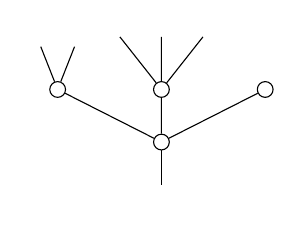
\begin{tikzpicture}[grow=up, every node/.style = {font=\footnotesize},level distance = 1.9em]%
	\tikzstyle{level 2}=[sibling distance=3.75em]%
	\tikzstyle{level 3}=[sibling distance=1.5em]%
		\node {}%
			child{node [dummy] {}%
				child{node [dummy] {}}%
				child{node [dummy] {}%
					child{}%
					child{}%
					child{}%
				}%
				child{node [dummy] {}%
					child{node {} }%
					child{node {} }%
				}%
			};%
	\end{tikzpicture}%
\]%
encodes the operadic composition
\[
	\O(3) \times \O(2) \times \O(3) \times \O(0) \to \O(5)
\]
where the inputs $\O(3), \O(2), \O(3), \O(0)$ correspond to the nodes (i.e. circles) in the tree, with arity given by number of incoming edges (i.e. edges immediately above)
and the output $\O(5)$ has arity given by counting leaves (i.e. edges at the top, not capped by a node).
Similarly, the role of equivariant trees is, in the context of equivariant operads, to encode such operadic compositions together with fixed point compatibilities.  
A detailed introduction to equivariant trees can be found in \cite[\S 4]{Pe17}, where the second author develops the theory of equivariant dendroidal sets (which is a parallel approach to equivariant operads), though here we include a single representative example.
Let $G = \{ \pm 1, \pm i, \pm j, \pm k\}$ denote the group of quaternionic units 
and $G \geq H \geq K \geq L$ denote the subgroups %
$H = \langle j \rangle$, %
$K = \langle -1 \rangle$, %
$L = \{1\}$.
There is then a $G$-tree $T$ with 
\textit{expanded representation}
given by the two trees on the left below and
\textit{orbital representation}
given by the (single) tree on the right.
\begin{equation}\label{D6SMALLER EQ}
	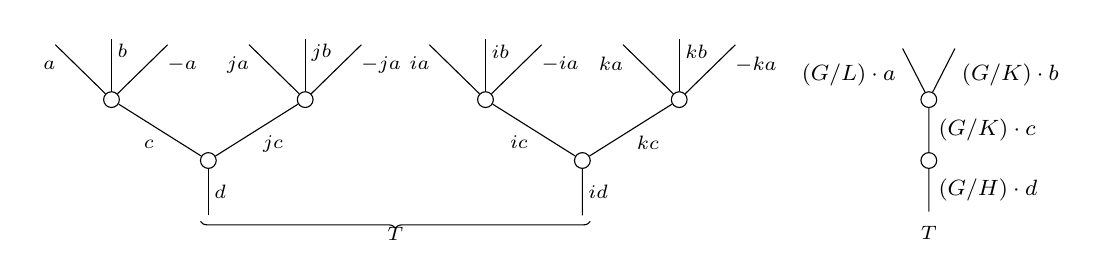
\begin{tikzpicture}[auto,grow=up, level distance = 2.2em,
	every node/.style={font=\scriptsize,inner sep = 2pt}]%
		\tikzstyle{level 2}=[sibling distance=7em]%
		\tikzstyle{level 3}=[sibling distance=2.25em]%
			\node at (4.75,0){}%	
				child{node [dummy] {}%
					child{node [dummy] {}%
						child{node {}%
						edge from parent node [swap,very near end] {$-k a$}}%
						child[level distance = 2.4em]{node {}%
						edge from parent node [swap,near end] {$k b$}}%
						child{node {}%
						edge from parent node [very near end] {$k a$}}%
					edge from parent node [swap] {$k c$}}%
					child{node [dummy] {}%
						child{node {}%
						edge from parent node [swap,very near end] {$-i a$}}%
						child[level distance = 2.4em]{node {}%
						edge from parent node [swap,near end] {$i b$}}%
						child{node {}%
						edge from parent node [very near end] {$i a$}}%
					edge from parent node  {$i c$}}%
				edge from parent node [swap] {$i d$}};%
			\node at (0,0){}%	
				child{node [dummy] {}%
					child{node [dummy] {}%
						child{node {}%
						edge from parent node [swap,very near end] {$-j a$}}%
						child[level distance = 2.4em]{node {}%
						edge from parent node [swap,near end] {$j b$}}%
						child{node {}%
						edge from parent node [very near end] {$j a$}}%
					edge from parent node [swap] {$j c$}}%
					child{node [dummy] {}%
						child{node {}%
						edge from parent node [swap,very near end] {$-a\phantom{j}$}}%
						child[level distance = 2.4em]{node {}%
						edge from parent node [swap,near end] {$b\phantom{j}$}}%
						child{node {}%
						edge from parent node [very near end] {$\phantom{j}a$}}%
					edge from parent node  {$\phantom{j}c$}}%
				edge from parent node [swap] {$d$}};%
		\begin{scope}[every node/.style={font=\footnotesize}]%
			\node at (9.15,0){}%
				child{node [dummy] {}%
					child{node [dummy] {}%
						child{node {}%
						edge from parent node [swap,very near end] {$(G/K) \cdot b$}}%
						child{node {}%
						edge from parent node [very near end] {$(G/L) \cdot a$}}%
					edge from parent node [right] {$(G/K) \cdot c$}}%
				edge from parent node [right] {$(G/H) \cdot d$}};%
		\end{scope}%
		\draw[decorate,decoration={brace,amplitude=2.5pt}] (4.85,0) -- (-0.1,0) node[midway]{$T$}; %
		\node at (9.15,-0.15) {$T$};
	\end{tikzpicture}%
\end{equation}%
We note that $G$ acts on the expanded representation of $T$ as indicated by the edge labels (so that the edges $a,b,c,d$ have stabilizers $L$, $K$, $K$, $H$ respectively), and the orbital representation is obtained by collapsing the edge orbits of the expanded representation. As explained in \cite[Example 4.9]{Pe17}, $T$ then encodes the fact that for any 
equivariant operad $\O \in \mathsf{Op}^G$ the composition 
$\mathcal{O}(2) \times \mathcal{O}(3)^{\times 2} \to 
\mathcal{O}(6)$ restricts to a fixed point composition
\begin{equation}\label{INTFIXPTCOMP EQ}
\O(H/K)^{H} \times \O(K/L \amalg K/K)^{K} \to
\O(H/L \amalg H/K)^{H}
\end{equation}
where $\O(X)$ for an $H$-set (resp. $K$-set) $X$ denotes $\O(|X|)$ together with a suitably intertwined $H$-action ($K$-action).
We note that the inputs 
$\O(H/K)^{H}$, $\O(K/L \amalg K/K)^{K}$ in
(\ref{INTFIXPTCOMP EQ})
correspond to the nodes of the orbital representation
in (\ref{D6SMALLER EQ}), though in contrast to the non-equivariant case arity is now determined by both incoming and outgoing edge orbits, while the output 
$\O(H/L \amalg H/K)^{H}$
is similarly determined by both the leaf and root edge orbits.
The existence of maps of the form (\ref{INTFIXPTCOMP EQ}) is essentially tantamount to the subtlest 
closure property for indexing systems $\mathcal{F}$,
self-induction (cf. \cite[Def. 3.20]{BH15}),
and similar tree descriptions exist for all other closure properties, as detailed by the second author in 
\cite[\S 9]{Pe17}.


We can now finally give a complete informal description of the category $\mathsf{Op}_G$ featured in 
our main result Theorem \ref{MAINQUILLENEQUIV THM}.
A genuine equivariant operad
$\mathcal{P} \in \mathsf{Op}_G$
has levels $\mathcal{P}(X)$ for each $H$-set $X$, $H\leq G$, 
that mimick the role of the fixed points $\O(X)^H$ for 
$\mathcal{O} \in \mathsf{Op}^G$.
More explicitly, there are restriction maps 
$\mathcal{P}(X) \to \mathcal{P}(X|_{K})$ for $K \leq L$,
isomorphisms
$\mathcal{P}(X)\simeq \mathcal{P}(g X)$
where $gX$ denotes the conjugate $gHg^{-1}$-set,
and composition maps of the form %, for example,
\[
\P(H/K) \times \P(K/L \amalg K/K) \to \P(H/L \amalg H/K)
\]
as in (\ref{INTFIXPTCOMP EQ}); in general, we have maps
%and multiplication maps
%\begin{align*}%\label{FIXEDPOINTMUL EQ}
\[
\begin{tikzcd}
  \mathcal{P}(H/K_1 \amalg \cdots \amalg H/K_n)
  \times
  \mathcal{P}(K_1 / L_{11} \amalg \cdots \amalg K_1/L_{1 m_1})
  \times \cdots \times
  \mathcal{P}(K_n / L_{n1} \amalg \cdots \amalg K_n / L_{n m_n})
  \arrow[d]
  \\
  % \to & 
  \mathcal{P}(H / L_{11} \amalg \cdots \amalg H/L_{1 m_1}
  \amalg \cdots \amalg
  H / L_{n1} \amalg \cdots \amalg H/L_{n m_n}
  )
\end{tikzcd}
\]
%\end{align*}
%generalizing (\ref{INTFIXPTCOMP EQ}) (which corresponds to the case $n=1$, $m_1 = 2$, $L_1 = L$, $L_2 = K$).
Lastly, thse composition maps %(\ref{FIXEDPOINTMUL EQ})
must satisfy associativity, unitality, and compatibility with restriction maps (noting that this will often change the orbit structure, radically altering the form of the given composition map) and equivariance conditions as encoded by the theory of $G$-trees. Rather than making such compatibilities explicit, it will be more convenient and effective for our purposes to simply define genuine equivariant operads intrinsically in terms of $G$-trees.



\subsection{Main results}


{\color{red} HERE}

We now present the highlights of this paper. 
%, each of which proves the existence of certain model structures, or makes comparisons between them. 
For much of the discussion, our base category will need to been sufficiently nice, either (Cartesian) \textit{strongly cellular} or \textit{underlying strongly cellular} (see Definitions \ref{STRONGLY_CELLULAR} and \ref{UNDERLYING_STRONGLY_CELLULAR}). In particular, these results all hold when $\V = \sSet$.

Our first result, proved in Section \ref{G_OP_EXISTS_SECTION}, shows that $G$-operads have a large variety of partial-genuine semi-model structures.

\begin{customthm}{I}\label{MAINEXIST1 THM}
Let $\V$ be strongly cellular, and fix $\F = \set{\F_n}$ a collection of sets $\F_n$ of subgroups of $G\times \Sigma_n$, each closed under conjugation. 
Then $\mathcal{F}$-semi-model structures, 
denoted
$\mathsf{Op}^G_{\mathcal{F}}(\mathcal{V})$,
on 
the category $\mathsf{Op}^G(\mathcal{V})$ exist.

If moreover $\V$ is underlying strongly cellular, these are actual model structures.
\end{customthm}

While we note that the above hold for general sets of subgroups of $G\times \Sigma_n$, when considering our genuine $G$-operads, we must restrict to collections $\F = \set{\F_n}$ of sets of graph subgroups, or equivalently full subcategories $\Sigma_\F$ of $\Sigma_G$. Letting $\Op_\F(\V)$ denote the category of $\mathbb F_G$-algebras in $\Sym_\F(\V)$, we have the following, proved in Section \ref{OP_G_EXISTS_SECTION}.

\begin{customthm}{II}\label{MAINEXIST2 THM}
Let $\V$ be Cartesian strongly cellular, and fix any full $\Sigma_\F \subseteq \Sigma_G$.
The projective semi-model structure on  
$\mathsf{Op}_{\mathcal{F}}(\mathcal{V})$ exist. 
Equivalently, the $\Sigma_\F$-semi-model structure, denoted $\Op_G^\F(\V)$, on $\Op_G(\V)$ exists.

If moreover $\V$ is underlying strongly cellular, these are actual model structures.
\end{customthm}

While these model structures always exist, they are not necessarily well-behaved with respect to cofibrancy unless the collections $\F$ are highly structured.
Our main result is the following, proved in Section \ref{MAINTHM_PROOF_SECTION}.

\begin{customthm}{III}\label{MAINQUILLENEQUIV THM}
Let $\mathcal{V}$ be $\mathsf{sSet}$ or, more generally, a Cartesian (underlying) strongly cellular model category.
%a strongly cofibrantly generated cartesian closed monoidal model category with cellular fixed points and with cofibrant symmetric pushout powers.

Then the adjunction 
\begin{equation}
\begin{tikzcd}[column sep =5em]
	\mathsf{Op}_G(\mathcal{V}) \ar[shift left=1.5]{r}{\iota^{\**}} 
	&
	\mathsf{Op}^G(\mathcal{V})
	\ar[shift left=1.5]{l}{\iota_{\**}} .
\end{tikzcd}
\end{equation}
is a Quillen equivalence.

More generally, for $\mathcal{F}$ a (weak) indexing system, 
the analogue adjunction 
\begin{equation}
\begin{tikzcd}[column sep =5em]
	\mathsf{Op}_{G}^{\mathcal F}(\mathcal{V}) \ar[shift left=1.5]{r}{\iota^{\**}} 
	&
	\mathsf{Op}^G_{\mathcal{F}}(\mathcal{V})
	\ar[shift left=1.5]{l}{\iota_{\**}} .
\end{tikzcd}
\end{equation}
is also a Quillen equivalence.
\end{customthm}

We lastly return to the conjecture of \cite{BH15}, which we resolve in the affirmative using two different methods in Section \ref{NINFTY_SECTION}.

\begin{customcor}{IV}\label{NINFTY_REAL_COR_MAIN}
For $\V = \sSet$ and 
$\mathcal{F} = \{\mathcal{F}_n\}_{n \geq 0}$
any weak indexing system,
$N \mathcal{F}$-operads exist. That is, there exist operads $\O$
such that
\begin{equation}%\label{NFINFTY EQ}
	\O(n)^{\Gamma} \sim 
\begin{cases}
	\** & \text{if } \Gamma \in \mathcal{F}_n
\\
	\emptyset & \text{otherwise}.
\end{cases}
\end{equation}  
In particular, $\mathrm{Ho}(N_\infty$-$\Op) \to \mathbb I$ is an equivalence of categories.%, proving Conjecture \ref{N_INFINITY_REALIZATION_CONJ}.
\end{customcor}

\subsection{Outline}

\todo[inline]{come back here}

% Much of this paper is dedicated to constructing the underlying categorical machinery used to run our investigation. 
% There are multiple distinct steps along the path to proving our main result:
% \begin{itemize}
% \item Defining $\mathbb F_G$, and rigorously showing it is a monad on $\Sym_G(\V)$ (Section \ref{GENUINE_OP_MONAD_SECTION}).
% \item Conveniently expressing free $\mathbb F_G$-extensions (Section \ref{FREE_EXTENSIONS_SECTION}).
% \item Analyzing filtrations of free $\mathbb F_G$-extensions to build various model structures (Section \ref{MODEL_STRUCTURES_SECTION}).
% \item Exploring the interplay between grafting of trees and cofibrancy to prove the above model structures are well-behaved (Section \ref{COFIB SEC}).
% \end{itemize}

% Much of the machinery in Sections \ref{GENUINE_OP_MONAD_SECTION} and \ref{FREE_EXTENSIONS_SECTION} are built in large categorical generality, designed such that the intuitive descriptions of, for example, the free operad monad and operations on forests, are verified with strict categorical rigor; as such, they may be of broader interest.
% %%%%%%%%%%%%%%%%%%%%%%%%%%%%%%%%%%%%%%%%%%%%%%%%%

% In particular, in order to arrive at this result, we need a better understanding of the interplay between the subtle equivariance structures we just discussed, and the combinatorics which underly operads. 
% That is, we need to synthesize the equivariant stories of \cite{Elm83, Pia91, Ste16} with the operadic story of \cite{MW07}, specifically building a suitable replacement for the notion of ``coefficient systems'' for operads over some ``nice'' base category $\V$.

% To that end, we exploit the equivariant generalization $\Omega_G$ of the dendroidal category $\Omega$ discussed in \cite{Pe17}.
% First, we observe that the free operad $\mathbb F X$ generated by a symmetric sequence $X \in \Sym(\V) = \V^\Sigma$, found in \cite{Spitz01, BM03}, can be repackaged as the left-most left Kan extension
% \[
% \begin{tikzcd}
%         |[alias=U]| \Omega^{op} \arrow[d, "\mathsf{lr}"'] \arrow[r, "N_X"] & \V & \qquad & |[alias=A]| \Omega_G^{op} \arrow[d, "\mathsf{lr}"'] \arrow[r, "N_Y"] & \V\\
%         \Sigma^{op} \arrow[ur, "\mathbb F X"', ""{name=V}] & && \Sigma_G^{op} \arrow[ur, "\mathbb F_G Y"', ""{name=B}]
%         \arrow[Rightarrow, from=U, to=V] 
%         \arrow[Rightarrow, from=A, to=B]
% \end{tikzcd}
% \]
% where $\mathsf{lr}$ is the ``leaf-root'' or ``valence'' functor, and $N_X$ sends $T$ to $\prod_{v\in V(T)} X(v)$.

% We generalize this to the equivariant setting using our $G$-trees $\Omega_G$ and $G$-corollas $\Sigma_G$ from \cite{Pe17}, and define an endofuctor $\mathbb F_G$ on the category of $G$-symmetric sequences $\Sym_G(\V) = \V^{\Sigma_G^{op}}$ by the right-most left Kan extension above; here, $\mathsf{lr}$ is the equivariant leaf-root functor.

\subsection{Future Work}

\todo[inline]{come back here}

% We end this introduction with a brief discussion on the general context of ``$G$-infinity operads''. We recall that $\infty$-operads, intuitively, can be thought of as operads where composition is ``weakly defined'', and $G$-coefficient systems spaces with a ``relaxed'' fixed-point condition. In this fashion, genuine $G$-operads can be thought of as $G$-operads where composition is still rigidly defined, but with relaxed fixed-point conditions. Comparitively, the $G$-$\infty$-operads of \cite{Pe17} have rigid fixed-point conditions but weak composition. The remaining missing link is a suitable notion of $G$-$\infty$-operad in the true pre-sheaf category $\Set^{\Omega_G^{op}}$:
% \[
% \begin{tikzcd}
%         \Op^G_\F(\V) \arrow[r, "i_*", "\simeq_Q"'] \arrow[d, "hcN^G"', "\simeq_Q ?"] & \Op_G^\F(\V) \arrow[d, "hcN_G", "\simeq ?"']\\
%         \mathsf{dSet}^G_\F \arrow[r, "i_*"', "\simeq_Q ?"] & \mathsf{dSet}_G^\F
% \end{tikzcd}
% \]
% We expect to make a full comparison between these notions in sequels.


\section{Preliminaries}

This section lists some elementary concepts
and results that will be used throughout the paper,
but may not be entirely standard.

\subsection{Grothendieck constructions}


Recall that for a diagram category $\mathcal{D}$ and functor $\mathcal{I}_{\bullet}$
\begin{equation}
\begin{tikzcd}[row sep = 0.2em]
	\mathcal{D} \ar{r}{\mathcal{I}_{\bullet}} & \mathsf{Cat} \\
	d \ar[mapsto]{r} & \mathcal{I}_d
\end{tikzcd}
\end{equation}
the (covariant) Grothendieck construction 
$\mathcal{D} \ltimes \mathcal{I}_{\bullet}$
has objects pairs $(d,i)$ with $d \in \mathcal{D}$,
 $i \in \mathcal{I}_d$ and 
arrows $(d,i) \to (d',i')$ given by pairs
\[(f\colon d \to d', g \colon f_{\**}(i) \to i'),\]
where $f_{\**}\colon \mathcal{I}_d \to \mathcal{I}_{d'}$ is a shorthand for the functor $\mathcal{I}_{\bullet}(f)$.


We now discuss a basic property of over and under categories that will be used in Section \ref{TRANSFSIMP SEC}.


Given $\mathcal{J},\C \in \mathsf{Cat}$ and $j \in \mathcal{J}$ we will let $\C^{ \downarrow j}$ denote the Grothendieck construction for the functor
\[
\begin{tikzcd}[row sep = 0.25em]
	\mathcal{J} \ar{r} & \mathsf{Cat} \\
	i \ar[mapsto]{r} & \C^{\mathcal{J}(i,j)}
\end{tikzcd}
\]
Explicitly, an object of $\C^{\downarrow j}$ is a pair
$\left(i,\mathcal{J}(i,j)\xrightarrow{\varphi} \C\right)$
and an arrow 
$(i,\varphi) \to (i',\varphi')$
is a pair
$(I \colon i \to i', 
\gamma \colon \varphi\circ I^{\**} \to \varphi')$.

	

\begin{lemma}\label{UNDERLEFTADJ LEM}
Let $\mathcal{J} \in \mathsf{Cat}$ be a small category and 
$j \in \mathcal{J}$. One then has adjunctions
\[
	(\minus \downarrow j) 
		\colon
	\mathsf{Cat}_{/\mathcal{J}}
		\rightleftarrows
	\mathsf{Cat}
		\colon
	(\minus)^{\downarrow j},
\qquad
	(j \downarrow \minus) 
		\colon
	\mathsf{Cat}_{/\mathcal{J}}
		\rightleftarrows
	\mathsf{Cat}
		\colon
	(\minus)^{j \downarrow}.
\]
\end{lemma}

\begin{proof}
Since $j \downarrow \mcI = (\mcI^{op} \downarrow j)^{op}$ by  defining $(\C^{j \downarrow}) = ((\C^{op})^{\downarrow j})^{op}$ one reduces to the leftmost adjuntion.

	Given $\mcI \xrightarrow{\pi} \mathcal{J}$ and $\C$ we will show that functors 
	$\mathcal{I} \downarrow j \xrightarrow{F} \C$
correspond to functors
	$\mathcal{I} \xrightarrow{G} \C^{\downarrow j}$ over $\mathcal{J}$.
	
	On objects, $F$ associates to each pair 
	$(i,J\colon \pi(i) \to j)$ an object $F(i,J)\in \C$. One thus sets $G(i)=(\pi(i), F(i,\minus))$ and these are clearly inverse processes.

	On arrows $F$ associates to 
	$(i,J' \circ \pi(I)) \xrightarrow{I} (i',J')$ an arrow
	$F(i,J' \circ \pi(I)) \xrightarrow{F(I)} F(i',J')$.
	One thus defines
\[
	G(I) = \left(
	\pi(i) \xrightarrow{\pi(I)} \pi(i'),
	F\left(i,(\minus)\circ \pi(i)\right)
		\xrightarrow{F(I)}
	F\left(i',\minus \right)
	\right)
\]
and again it is clear that these are inverse processes.
	Finally, the fact that the associativity and unit conditions for $F,G$ coincide is likewise clear.
\end{proof}



\subsection{Monads}

We will make multiple uses of the following straightforward results.

\begin{proposition}\label{MONADADJ1 PROP}
Let
$
L \colon \mathcal{C} \rightleftarrows \mathcal{D} \colon R
$
be an adjunction and $T$ a monad on $\mathcal{D}$.
Then
\begin{itemize}
\item[(i)] $RTL$ is a monad and $R$ induces a functor
$R \colon \mathsf{Alg}_T(\mathcal{D}) \to \mathsf{Alg}_{RTL}(\mathcal{C})$;
\item[(ii)] if $LRTL \xrightarrow{\epsilon} TL$ is an isomorphism one further has an induced adjunction
\[
L \colon \mathsf{Alg}_{RTL}(\mathcal{C})
	\rightleftarrows
\mathsf{Alg}_{T}(\mathcal{D}) \colon R.
\]
\end{itemize}
\end{proposition}



\begin{proposition}\label{MONADADJ PROP}
Let
$
L \colon \mathcal{C} \rightleftarrows \mathcal{D} \colon R
$
be an adjunction, $T$ a monad on $\mathcal{C}$, and suppose further that
\[
	LR \xrightarrow{\epsilon} id_{\mathcal{D}}, 
\qquad
	LT \xrightarrow{\eta} LTRL
\]
are natural isomorphisms 
(so that in particular $\mathcal{D}$ is a reflexive subcategory of $\mathcal{C}$).

Then
\begin{itemize}
\item[(i)] $LTR$ is a monad, with multiplication and unit given by
\[LTRLTR \xrightarrow{\eta^{-1}} LTTR \to LTR,\qquad
id_{\mathcal{D}} \xrightarrow{\epsilon^{-1}} LR \to LTR;
\]
\item[(ii)]
$d \in \mathcal{D}$ is a $LTR$-algebra iff $Rd$ is a $T$-algebra;
\item[(iii)] there is an induced adjunction
\[
L \colon \mathsf{Alg}_{T}(\mathcal{C})
	\rightleftarrows
\mathsf{Alg}_{LTR}(\mathcal{D}) \colon R.
\]
\end{itemize}
\end{proposition}









\section{Planar and tall maps}

\subsection{Planar structures}


Throughout we will work with trees possessing \textit{planar structures} or, more intuitively, trees embedded into the plane.

Our preferred model for trees will be that of broad posets first introduced by Weiss in \cite{We12} and further worked out by the second author in \cite{Pe17}. We now define planar structures in this context.


\begin{definition}\label{PLANARIZE DEF}
	Let $T \in \Omega$ be a tree. A \textit{planar structure} of $T$ is an extension of the descendancy partial order $\leq_d$ to a total order $\leq_p$ such that: 
	\begin{itemize}
		\item \textit{Planar}: if $e \leq_p f$ and $e \nleq_d f$ then 
		$g \leq_d f$ implies $e \leq_p g$.
	\end{itemize} 
\end{definition}


\begin{example}
An example of a planar structure on a tree $T$ follows, with $\leq_r$ encoded by the number labels.
\begin{equation}\label{PLANAREX EQ}
	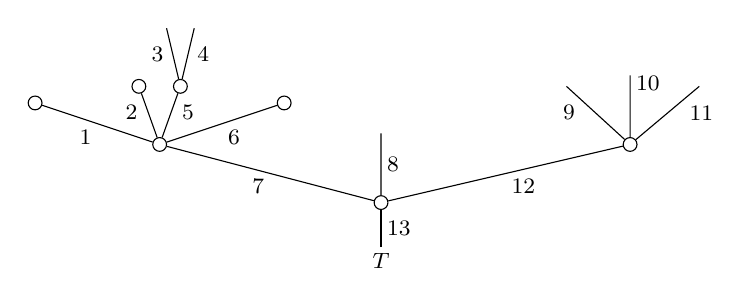
\begin{tikzpicture}[grow=up,auto,level distance=2.1em,
	every node/.style = {font=\footnotesize,inner sep=2pt},
	dummy/.style={circle,draw,inner sep=0pt,minimum size=1.75mm}]
		\node at (0,0) {$T$}
			child{node [dummy] {}
				child[sibling distance = 9em]{node [dummy] {}
					child[sibling distance = 2.5em]{
					edge from parent node [near end,swap] {$11$}}
					child[level distance=2.5em]{
					edge from parent node [very near end,swap] {$10$}}				
					child[sibling distance = 2.3em]{
					edge from parent node [near end] {$9$}}
				edge from parent node [swap] {12}}
				child[level distance =2.5em]{
				edge from parent node [swap] {$8$}}
				child[sibling distance = 8em]{node [dummy] {}
					child[sibling distance =3em, level distance = 1.5 em]{node [dummy] {}
					edge from parent node [swap] {$6$}}
					child[sibling distance = 1.5em]{node [dummy] {}
						child[sibling distance =1em]{
						edge from parent node [swap,near end] {$4$}}
						child[sibling distance =1em]{
						edge from parent node [near end] {$3$}}
					edge from parent node [very near end,swap] {$5$}}
					child[sibling distance =1.5em]{node [dummy] {}
					edge from parent node [very near end] {$2$}}
					child[sibling distance =3em,level distance =1.5em]{node [dummy] {}
					edge from parent node {$1$}}
				edge from parent node {$7$}}
			edge from parent node [swap] {$13$}};
	\end{tikzpicture}
\end{equation}
Intuitively, given a planar depiction of a tree $T$, $e \leq_d f$ holds when the downward path from $e$ passes through $f$
and $e \leq_p f$ holds if either
$e \leq_d f$ or if the downward path from $e$ is to the left of the downward path from $f$ (as measured at the node where the paths intersect).
\end{example}



Intuitively, a planar depiction of a tree amounts to choosing a total order for each of the sets of \textit{input edges} of each node (i.e. those edges immediately above that node).

While we will not need to make this last statement precise, we will nonetheless find it convenient to show that Definition \ref{PLANARIZE DEF} is equivalent to such choosing total orders for each of the sets of input edges.
To do so, we first introduce some notation.


\begin{notation}\label{INPUTPATH NOT}
	Let $T \in \Omega$ be a tree and $e \in T$ and edge. We will denote
	\[ I(e) =\{f \in T \colon e \leq_d f \} \]
and refer to this poset as the \textit{input path of $e$}.
\end{notation}

We will repeatedly use the following, which is a consequence of \cite[Cor. 5.26]{Pe17}.

\begin{lemma}\label{INCOMPNOTOP}
If $e \leq_d f$, $e \leq_d f'$, then $f,f'$ are $\leq_d$-comparable. 
\end{lemma} 

\begin{proposition}\label{INPUTPATHS PROP}
	Let $T \in \Omega$ be a tree. Then
	\begin{itemize}
		\item[(a)] for any $e \in T$ the finite poset $I(e)$ is totally ordered;
		\item[(b)] the poset $(T,\leq_d)$ has all joins, denoted $\vee$. In fact, $\bigvee_{i} e_i = \min (\bigcap_{i} I(e_i))$.
	\end{itemize}
\end{proposition}

\begin{proof}
	(a) is immediate from Lemma \ref{INCOMPNOTOP}.
To prove (b) we note that 
	$\min (\bigcap_{i} I(e_i))$ exists by (a), and that this is clearly the join $\bigvee{e_i}$.
\end{proof}


\begin{notation}
	Let $T \in \Omega$ be a tree and suppose that $e <_d b$. We will denote by $b^{\uparrow}_e \in T$ the predecessor of $b$ in $I(e)$.
\end{notation}


\begin{proposition}\label{INPUTPREDECESSORPROP PROP}
Suppose $e,f$ are $\leq_d$-incomparable edges of $T$ and write $b= e \vee f$. Then
\begin{itemize}
\item [(a)] $e <_d b$, $f<_d b$ and $b^{\uparrow}_e \neq b^{\uparrow}_f$;
\item [(b)] $b^{\uparrow}_e, b^{\uparrow}_f \in b^{\uparrow}$. In fact $\{b^{\uparrow}_e\} = I(e) \cap b^{\uparrow}$,
$\{b^{\uparrow}_f\} = I(f) \cap b^{\uparrow}$;
\item[(c)] if $e' \leq_d e$, $f' \leq_d f$ then 
$b = e' \vee f'$ and $b^{\uparrow}_{e'} = b^{\uparrow}_{e}$, $b^{\uparrow}_{f'} = b^{\uparrow}_{f}$.
\end{itemize}
\end{proposition}


\begin{proof}
(a) is immediate: the condition $e = g$ (resp. $f = g$) would imply $f \leq_d e$ (resp. $e \leq_d f$)
while the condition $b^{\uparrow}_e = b^{\uparrow}_f$ would provide a predecessor of $b$ in $I(e) \cap I(f)$. 

For (b), note that any relation $a <_d b$ factors as 
$a \leq_d b^{\star}_a <_d b$ for some unique $b^{\**}_a \in b^{\uparrow}$, where uniqueness follows from Lemma \ref{INCOMPNOTOP}. Choosing $a=e$ implies $I(e) \cap b^{\uparrow} = \{b^{\**}_e\}$ and letting $a$ range over edges such that $e \leq_d a <_d b$ shows that $b^{\**}_e$ is in fact the predecessor of $b$.

To prove (c) one reduces to the case $e'=e$, in which case it suffices to check $I(e) \cap I(f') = I(e) \cap I(f)$. But if it were otherwise there would exist an edge $a$ satisfying
$f' \leq_d a <_d f$ and $e \leq_d a$, and this would imply $e \leq_d f$, contradicting our hypothesis.
\end{proof}



\begin{proposition}
\label{TERNARYJOIN PROP}
Let $c = e_1 \vee e_2 \vee e_3$.
Then $c = e_i \vee e_j$ iff $c^{\uparrow}_{e_i} \neq c^{\uparrow}_{e_j}$.

Therefore, all ternary joins in $(T,\leq_d)$ are binary, i.e.
\begin{equation}\label{TERNJOIN EQ}
	c = e_1 \vee e_2 \vee e_3 = e_i \vee e_j
\end{equation}
for some $1\leq i <j \leq 3$, and
(\ref{TERNJOIN EQ}) fails for 
 at most one choice of $1\leq i <j \leq 3$.
\end{proposition}


\begin{proof}
If $c^{\uparrow}_{e_i} \neq c^{\uparrow}_{e_j}$ then
$c = \min\left(I(e_i) \cap I(e_j)\right) = e_i \vee e_j$, whereas the converse follows from Proposition \ref{INPUTPREDECESSORPROP PROP}(a).

The ``therefore'' part follows by noting that 
$c^{\uparrow}_{e_1}$, $c^{\uparrow}_{e_2}$, $c^{\uparrow}_{e_3}$
can not all coincide, or else $c$ would not be the minimum of
$I(e_1) \cap I(e_2) \cap I(e_3)$. 
\end{proof}


\begin{example} In the following example $b = e \vee f$, $c = e \vee f \vee g$, $c^{\uparrow}_e= c^{\uparrow}_f =b$.
\[
	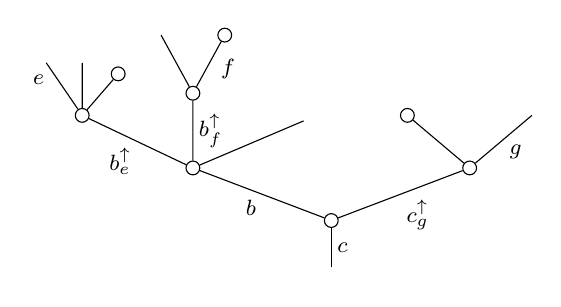
\begin{tikzpicture}[grow=up,auto,level distance=1.9em,
	every node/.style = {font=\footnotesize,inner sep=2pt},
	dummy/.style={circle,draw,inner sep=0pt,minimum size=1.75mm}]
		\node at (0,0) {}
			child{node [dummy] {}
				child[sibling distance = 10em]{node [dummy] {}
					child[sibling distance = 4.5em]{
					edge from parent node [swap] {$g$}}
					child[sibling distance = 4.5em]{node [dummy] {}}
				edge from parent node [swap] {$c_g^{\uparrow}$}}
				child[sibling distance = 10em]{node [dummy] {}
					child[sibling distance = 4em,level distance=1.7em]
					child[sibling distance = 1.5em,level distance=2.7em]{node [dummy] {}
						child[level distance=2.1em,sibling distance = 2.3em]{node [dummy] {}
						edge from parent node [near end,swap] {$f$}}		
						child[level distance=2.1em,sibling distance = 2.3em]{
						edge from parent node [near end] {}}
					edge from parent node [swap] {$b^{\uparrow}_{f}$}}
					child[sibling distance = 4em]{node [dummy] {}
						child[sibling distance =1.3em, level distance = 1.5 em]{node [dummy]  {}
						edge from parent node [swap] {}}
						child[sibling distance = 1.3em]{
						edge from parent node [very near end,swap] {}}
						child[sibling distance =1.3em]{
						edge from parent node [very near end] {$e$}}
					edge from parent node {$b^{\uparrow}_e$}}
				edge from parent node {$b$}}
			edge from parent node [swap] {$c$}};
	\end{tikzpicture}
\]
\end{example}

\begin{notation}
	Given a set $S$ of size $n$ we write
	$\textsf{Ord}(S) \simeq \mathsf{Iso}(S,\{1,\cdots,n\})$. We will usually abuse notation by regarding its objects as pairs $(S,\leq)$ where $\leq$ is a total order in $S$.
\end{notation}


\begin{proposition}\label{PLANARIZATIONCHAR PROP}
	Let $T \in \Omega$ be a tree. There is a bijection
	\begin{equation}\label{PLANAR EQ}
	\begin{tikzcd}[row sep = 0.5em]
		\{\text{planar structures }(T,\leq_p)\} \ar[r] &
		\prod_{(a^{\uparrow} \leq a) \in V(T)} \mathsf{Ord}(a^{\uparrow}) \\
		\leq_p \ar[mapsto]{r} & (\leq_p|_{a^{\uparrow}})
	\end{tikzcd}	
	\end{equation}
\end{proposition}


\begin{proof}
We will keep the setup of Proposition \ref{INPUTPREDECESSORPROP PROP} throughout: $e, f$ are $\leq_d$-incomparable edges and we write $b = e \vee f$. 

	We first show that (\ref{PLANAR EQ}) is injective, i.e. that the restrictions $\leq_p|_{a^{\uparrow}}$ determine if 
	$e <_p f$ holds or not.
If $b^{\uparrow}_e <_p b^{\uparrow}_f$, the relations
$e \leq_d b^{\uparrow}_e <_p b^{\uparrow}_f \geq_d f$
and Definition \ref{PLANARIZE DEF} imply it must be $e <_p f$.
Dually, if $b^{\uparrow}_f <_p b^{\uparrow}_e$ then 
$f <_p e$. Thus 
$b^{\uparrow}_e <_p b^{\uparrow}_f \Leftrightarrow e <_p f$ and hence (\ref{PLANAR EQ}) is indeed injective.

To check that (\ref{PLANAR EQ}) is surjective, it suffices (recall that $e,f$ are assumed $\leq_d$-incomparable) to check that
defining $e \leq_p f$ to hold iff $b^{\uparrow}_e < b^{\uparrow}_f$ holds in $b^{\uparrow}$ yields a planar structure.

Antisymmetry and the total order conditions are immediate, and it thus remains to check the transitivity and planar conditions.
Transitivity of $\leq_p$ in the case $e' \leq_d e <_p f$ and the planar condition, which is the case $e <_p f \geq_d f'$, follow from Proposition \ref{INPUTPREDECESSORPROP PROP}(c). Transitivity of $\leq_p$ in the case $e <_p f \leq_d f'$
follows since either $e \leq_d f'$ or else $e,f'$ are $\leq_d$-incomparable, in which case one can apply \ref{INPUTPREDECESSORPROP PROP}(c) with the roles of $f,f'$ reversed.

It remains to check transitivity in the hardest case, that of 
$e <_p f <_p g$ with $\leq_d$-incomparable $f,g$.
We write $c = e \vee f \vee g$.
By the ``therefore'' part of Proposition \ref{TERNARYJOIN PROP}, either
\begin{inparaenum}
	\item[(i)] $e \vee f <_d c$, in which case 
	Proposition \ref{TERNARYJOIN PROP}
	implies 
	$c^{\uparrow}_e = c^{\uparrow}_f$ and transitivity follows;
	\item[(ii)] $f \vee g <_d c$, which follows just as (i);
	\item[(iii)]  
$e \vee f = f \vee g =c$, in which case 
$c^{\uparrow}_e <
c^{\uparrow}_f <
c^{\uparrow}_g $ in $c^{\uparrow}$
so that $c^{\uparrow}_e \neq c^{\uparrow}_g$ and by Proposition \ref{TERNARYJOIN PROP} it is also 
$e \vee g = c$ and transitivity follows.
\end{inparaenum}
\end{proof}


\begin{remark}\label{FORESTPLAN REM}
	Definition \ref{PLANARIZE DEF} readily extends to forests $F \in \Phi$. The analogue of Proposition \ref{PLANARIZATIONCHAR PROP} then states that the data of a planar structure is 
equivalent to total orderings of the nodes of $F$ together with a total ordering of its set of roots.
Indeed, this follows by either adapting the proof above or by noting that planar structures on $F$ are clearly in bijection with planar structures on the join tree $F \star \eta$ 
(cf. \cite[Def. 7.44]{Pe17}), which adds a single edge $\eta$ to $F$, serving as the (unique) root of $F \star \eta$.
\end{remark}


When discussing the substitution procedure in Section \ref{SUBS SEC} we will find it convenient to work with a model for the category $\Omega$ that possesses exactly one representative of each possible planar structure on each tree or, more precisely, such that the only isomorphisms preserving the planar structures are the identities. On the other hand, using such a model for $\Omega$ throughout would, among other issues, make the discussion of faces in Section \ref{OUTTALL SEC} rather awkward.
We now outline our conventions to address such issues.


Let $\Omega^p$, the category of \textit{planarized trees}, denote the category with objects pairs $T_{\leq_p}=(T,\leq_p)$ of trees together with a planar structure  and morphisms the \textit{underlying} maps of trees (so that the planar structures are ignored).
There is a full subcategory $\Omega^s \hookrightarrow \Omega^p$, whose objects we call \textit{standard models}, of those $T_{\leq_p}$ whose underlying set is one of the sets $\underline{n} = \{1,2,\cdots,n\}$ and for which $\leq_p$ coincides with the canonical order. 
\begin{example}\label{STANDMODEL EX}
	Some examples of standard models, i.e. objects of $\Omega^s$, follow (further, (\ref{PLANAREX EQ}) can also be interpreted as such an example).
\begin{equation}\label{PLANAROMEGAEX1 EQ}
	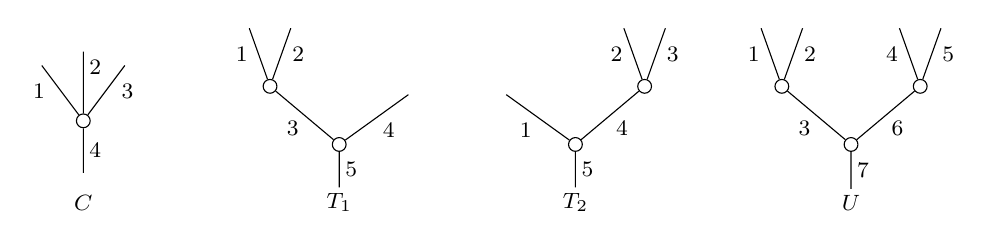
\begin{tikzpicture}[grow=up,auto,level distance=2.1em,
	every node/.style = {font=\footnotesize,inner sep=2pt},
	dummy/.style={circle,draw,inner sep=0pt,minimum size=1.75mm}]
		\node at (-0.25,0) {$C$};
		\node at (-0.25,0.3) {}
			child{node [dummy] {}
				child[sibling distance = 1.5em,level distance= 2em]{
				edge from parent node [swap, near end] {$3$}}
				child[sibling distance = 1.5em,level distance= 2.5em]{
				edge from parent node [swap, near end] {$2$}}
				child[sibling distance = 1.5em,level distance= 2em]{
				edge from parent node [near end] {$1$}}
			edge from parent node [swap] {$4$}};
		\node at (3,0) {$T_1$}
			child{node [dummy] {}
				child[sibling distance = 5em, level distance=1.8em]{
				edge from parent node [swap] {$4$}}
				child[sibling distance = 5em]{node [dummy] {}
					child[sibling distance = 1.5em]{
					edge from parent node [swap,near end] {$2$}}
					child[sibling distance = 1.5em]{
					edge from parent node [near end] {$1$}}
				edge from parent node {$3$}}
			edge from parent node [swap] {$5$}};
		\node at (6,0) {$T_2$}
			child{node [dummy] {}
				child[sibling distance = 5em]{node [dummy] {}
					child[sibling distance = 1.5em]{
					edge from parent node [swap,near end] {$3$}}
					child[sibling distance = 1.5em]{
					edge from parent node [near end] {$2$}}
				edge from parent node [swap] {$4$}}
				child[sibling distance = 5em, level distance=1.8em]{
				edge from parent node {$1$}}
			edge from parent node [swap] {$5$}};
		\node at  (9.5,0) {$U$}
			child{node [dummy] {}
				child[sibling distance = 5em]{node [dummy] {}
					child[sibling distance = 1.5em]{
					edge from parent node [swap,near end] {$5$}}
					child[sibling distance = 1.5em]{
					edge from parent node [near end] {$4$}}
				edge from parent node [swap] {$6$}}
				child[sibling distance = 5em]{node [dummy] {}
					child[sibling distance = 1.5em]{
					edge from parent node [swap,near end] {$2$}}
					child[sibling distance = 1.5em]{
					edge from parent node [near end] {$1$}}
				edge from parent node {$3$}}
			edge from parent node [swap] {$7$}};
	\end{tikzpicture}
\end{equation}
Here $T_1$ and $T_2$ are isomorphic to each other but not isomorphic to any other standard model in $\Omega^s$ while both $C$ and $U$ are the unique objects in their isomorphism classes. 
\end{example}


Given $T_{\leq_p} \in \Omega^p$ there is an obvious standard model $T_{\leq_p}^s \in \Omega^s$ given by replacing each edge by its order following $\leq_p$. Indeed, this defines a retraction 
$(\minus)^s \colon \Omega^p \to \Omega^s$
and a natural transformation 
$\sigma \colon id \Rightarrow (\minus)^s$
given by isomorphisms preserving the planar structure
(in fact, the pair $\left((\minus)^s, \sigma \right)$ is clearly unique).


\begin{convention}\label{PLANARCONV CON}
	From now on, we will write simply $\Omega$, $\Omega_G$ to denote the categories $\Omega^s$, $\Omega_G^s$ of standard models (where planar structures are defined in the underlying forest as in Remark \ref{FORESTPLAN REM}). 
Similarly $\mathsf{O}_G$ will denote the model $\mathsf{O}_G^s$ for the orbital category whose objects are the orbital $G$-sets whose underlying set is one of the sets $\underline{n} = \{1,2,\cdots,n\}$.

Therefore, whenever one of our constructions produces an object/diagram in $\Omega^p$, $\Omega^p_G$, $\mathsf{O}_G^p$ (of trees, $G$-trees, orbital $G$-sets with a planarization/total order) we will hence implicitly reinterpret it by using the standardization functor $(\minus)^s$.
\end{convention}

\begin{example}
To illustrate our convention, we consider the trees in Example \ref{STANDMODEL EX}. 

One has subfaces
$F_1 \subset F_2 \subset U$
where $F_1$ is the subtree with edge set $\{1,2,6,7\}$ and 
$F_2$ is the subtree with edge set $\{1,2,3,6,7\}$, both with inherited tree and planar structures. 
Applying $(\minus)^s$ to the inclusion diagram on the left below then yields a diagram as on the right.
\[
\begin{tikzcd}[row sep = 0.5em,column sep =1.3em]
	F_1 \ar[hookrightarrow]{rr} \ar[hookrightarrow]{rd} & & U & &&
	C \ar{rr} \ar{rd} & & U
\\
	& F_2 \ar[hookrightarrow]{ru} & & &&
	& T_1 \ar{ru}
\end{tikzcd}
\]
Similarly, let $\leq_{(12)}$ and $\leq_{(45)}$ denote alternate planar structures for $U$ exchanging the orders of the pairs $1,2$ and $4,5$, so that one has objects 
$U_{\leq_{(12)}}$, $U_{\leq_{(45)}}$ in $\Omega^p$. 
Applying $(\minus)^s$ to the diagram of underlying identities on the left yields the permutation diagram on the right.
\[
\begin{tikzcd}[row sep = 0.5em,column sep =1.3em]
	U \ar{rr}{id} \ar{rd}[swap]{id} & & U_{\leq_{(45)}} & & &
	U \ar{rr}{(45)} \ar{rd}[swap]{(12)} & & U
\\
	& U_{\leq_{(12)}} \ar{ru}[swap]{id} & & & &
	& U \ar{ru}[swap]{(12)(45)}
\end{tikzcd}
\]
\end{example}

\begin{example}
An additional reason to leave the use of $(\minus)^s$ implicit
is that when depicting $G$-trees it is preferable to choose edge labels that describe the action rather than the planarization (which is already implicit anyway).

For example, when $G = \mathbb{Z}_{/4}$, in both diagrams below the orbital representation on the left represents the isomorphism class consisting of the two trees $T_1,T_2 \in \Omega_G$ on the right.
\[
	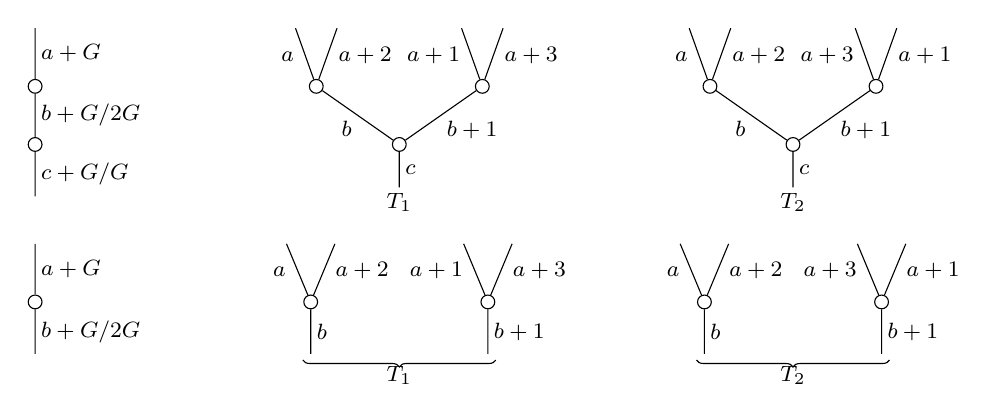
\begin{tikzpicture}[grow=up,auto,level distance=2.1em,
	every node/.style = {font=\footnotesize,inner sep=2pt},
	dummy/.style={circle,draw,inner sep=0pt,minimum size=1.75mm}]
		\node at (-1,0) {}
			child{node [dummy] {}
				child{node [dummy] {}
					child{
					edge from parent node [swap] {$a+G$}}
				edge from parent node [swap] {$b+G/2G$}}
			edge from parent node [swap] {$c + G/G$}};

		\node at  (3.625,0) {$T_1$}
			child{node [dummy] {}
				child[sibling distance = 6em]{node [dummy] {}
					child[sibling distance = 1.5em]{
					edge from parent node [swap,near end] {$a+3$}}
					child[sibling distance = 1.5em]{
					edge from parent node [near end] {$a+1$}}
				edge from parent node [swap] {$b+1$}}
				child[sibling distance = 6em]{node [dummy] {}
					child[sibling distance = 1.5em]{
					edge from parent node [swap,near end] {$a+2$}}
					child[sibling distance = 1.5em]{
					edge from parent node [near end] {$\phantom{0+}a$}}
				edge from parent node {$\phantom{1+}b$}}
			edge from parent node [swap] {$c$}};
		\node at  (8.625,0) {$T_2$}
			child{node [dummy] {}
				child[sibling distance = 6em]{node [dummy] {}
					child[sibling distance = 1.5em]{
					edge from parent node [swap,near end] {$a+1$}}
					child[sibling distance = 1.5em]{
					edge from parent node [near end] {$a+3$}}
				edge from parent node [swap] {$b+1$}}
				child[sibling distance = 6em]{node [dummy] {}
					child[sibling distance = 1.5em]{
					edge from parent node [swap,near end] {$a+2$}}
					child[sibling distance = 1.5em]{
					edge from parent node [near end] {$\phantom{0+}a$}}
				edge from parent node {$\phantom{1+}b$}}
			edge from parent node [swap] {$c$}};
		\node at (-1,-2) {}
			child{node [dummy] {}
				child[sibling distance=1.75em]{
				edge from parent node [swap]  {$a+G$}}
			edge from parent node [swap] {$b+G/2G$}};
		\node at (2.5,-2) {}
			child{node [dummy] {}
				child[sibling distance=1.75em]{
				edge from parent node [swap,near end] {$a+2$}}
				child[sibling distance=1.75em]{
				edge from parent node [near end]  {$\phantom{1+}a$}}
			edge from parent node [swap] {$b$}};
		\node at (4.75,-2) {}
			child{node [dummy] {}
				child[sibling distance=1.75em]{
				edge from parent node [swap,near end] {$a+3$}}
				child[sibling distance=1.75em]{
				edge from parent node [near end]  {$a+1$}}
			edge from parent node [swap] {$b+1$}};
		\draw[decorate,decoration={brace,amplitude=2.5pt}] (4.85,-2) -- (2.4,-2) node[midway]{$T_1$};
		\node at (7.5,-2) {}
			child{node [dummy] {}
				child[sibling distance=1.75em]{
				edge from parent node [swap,near end] {$a+2$}}
				child[sibling distance=1.75em]{
				edge from parent node [near end]  {$\phantom{1+}a$}}
			edge from parent node [swap] {$b$}};
		\node at (9.75,-2) {}
			child{node [dummy] {}
				child[sibling distance=1.75em]{
				edge from parent node [swap,near end] {$a+1$}}
				child[sibling distance=1.75em]{
				edge from parent node [near end]  {$a+3$}}
			edge from parent node [swap] {$b+1$}};
		\draw[decorate,decoration={brace,amplitude=2.5pt}] (9.85,-2) -- (7.4,-2) node[midway]{$T_2$};
	\end{tikzpicture}
\]
\end{example}


\begin{definition}
	A morphism $S \xrightarrow{\varphi} T$ in $\Omega$ that is compatible with the planar structures $\leq_p$ is called a 
	\textit{planar map}.
	
	More generally, a morphism $F \to G$ in the categories $\Phi$, $\Phi^G$, $\Omega^G$ of forests, $G$-forests, $G$-trees is called a \textit{planar map} if it is an independent map (cf. \cite[Def. 5.28]{Pe17}) compatible with the planar structures $\leq_p$.
\end{definition}


\begin{remark}
	The need for the independence condition is justified by \cite[Lemma 5.33]{Pe17} and its converse, since non independent maps do not reflect
 $\leq_d$ inequalities.
 
 We note that in the $\Omega_G$ case a map $\varphi$ is independent iff $\varphi$ does not factor through a non trivial quotient iff $\varphi$ is injective on each edge orbit.
\end{remark}


\begin{proposition}
\label{PLANARPULL EQ}
	Let $F \xrightarrow{\varphi} G$ be an independent map in $\Phi$ (or $\Omega$, $\Omega_G$, $\Phi_G$). Then there is a unique factorization 
	\[F \xrightarrow{\simeq} \bar{F} \to G\]
	such that $F \xrightarrow{\simeq} \bar{F}$ is an isomorphism and $\bar{F} \to G$ is planar.
\end{proposition}

\begin{proof}
We need to show that there is a unique planar structure 
$\leq_p^{\bar{F}}$ on the underlying forest of $F$ making the underlying map a planar map.
Simplicity of $G$ ensures that for any vertex $e^{\uparrow} \leq e$ of $F$ the edges in $\varphi(e^{\uparrow})$ are all distinct while independence of $\varphi$ likewise ensures that the edges in $\varphi(\underline{r}_F)$ are distinct.
The result now follows from (the forest version of) Proposition
\ref{PLANARIZATIONCHAR PROP}: one simply orders each set $e^{\uparrow}$ and $\underline{r}_F$ according to its image.

{\color{orange} not quite complete... maybe that $\leq_p$ is the closure of $\leq_d$ and the vertex relations under transitivity and the planar condition}
\end{proof}



\begin{remark}\label{PULLPLANAR REM}
	Proposition \ref{PLANARPULL EQ} says that planar structures  can be pulled back along independent maps. However, they can not always be pushed forward. As an example, in the notation of (\ref{PLANAROMEGAEX1 EQ}), consider the map $C \to T_1$ defined by $1 \mapsto 1$, $2 \mapsto 4$, $3 \mapsto 2$, $4 \mapsto 5$.
\end{remark}

\begin{remark}\label{UNIQCOR REM}
	Given any tree $T \in \Omega$ there is a unique corolla $\mathsf{lr}(T) \in \Sigma$ and planar tall map 
	$\mathsf{lr}(T) \to T$.
	Explicitly, the number of leaves of $\mathsf{lr}(T)$ matches that of $T$, together with the inherited order. 
\end{remark}

\todo[inline]{planarity for $\Omega_G$: choice of planar structures on $\amalg_{[g]}T_{[g]}$, $G\cdot_H T_H$, etc}

\subsection{Outer faces and tall maps}\label{OUTTALL SEC}



In preparation for our discussion of the substitution operation in Section \ref{SUBS SEC}, we now recall some basic notions and results concerning outer subtrees and tree grafting, as in \cite[Section 5]{Pe17}.

\begin{definition}
	Let $T \in \Omega$ be a tree and 
	$e_1 \cdots e_n =\underline{e} \leq e$ a broad relation in $T$.
	
	We define the \textit{planar outer face $T_{\underline{e} \leq e}$}
	to be the subtree with underlying set those edges $f \in T$ such that
\begin{equation}\label{OUTERFACE EQ}
	f \leq_d e,\quad \forall_i f \nless_d e_i,
\end{equation}
generating broad relations the relations $f^{\uparrow} \leq f$ for those $f \in T$ satisfying (\ref{OUTERFACE EQ}) but 
$\forall_i f\neq e_i$,
and planar structure pulled back from $T$.
\end{definition}


\begin{remark}
If one forgoes the requirement that $T_{\underline{e} \leq e}$ be equipped with the pullback planar structure, the inclusion $T_{\underline{e} \leq e} \to T$ is usually called simply an \textit{outer face}.
\end{remark}

We now recap some basic results.

\begin{proposition}
Let $T \in \Omega$ be a tree.
\begin{itemize}
\item[(a)] $T_{\underline{e} \leq e}$ is a tree with root $e$
and edge tuple $\underline{e}$;
\item[(b)] there is a bijection
\[
	\{\text{planar outer faces of $T$} \} 
\leftrightarrow 
	\{\text{broad relations of $T$}\};
\]
\item[(c)] if $R \to S$ and $S \to T$ are outer face maps then so is $R \to T$;
\item[(d)] any pair of broad relations $\underline{g} \leq v$, $\underline{f}v \leq e$ induces a grafting pushout diagram
\begin{equation}\label{GRAPTPUSH EQ}
\begin{tikzcd}
	\eta \ar{r}{v} \ar{d}[swap]{v} & T_{\underline{g} \leq v} \ar{d}
\\
	T_{\underline{f}v \leq e} \ar{r} & T_{\underline{f}\underline{g} \leq e}
\end{tikzcd}
\end{equation}
%\item[(e)] a face map $S \to T$ is an outer face map iff whenever the composite relation $\underline{f} \underline{g} \leq e$ is in $S$ then so are the relations $\underline{g} \leq v$ and
%$\underline{f}v \leq e$.
\end{itemize}
\end{proposition}


\begin{proof}
We first show (a). That $T_{\underline{e} \leq e}$ is indeed a tree is the content of \cite[Prop. 5.20]{Pe17}: more precisely, 
$T_{\underline{e} \leq e} = (T^{\leq e})_{\less \underline{e}}$
in the notation therein. That the root of $T_{\underline{e} \leq e}$ is $e$ is clear and that the root tuple is $\underline{e}$ follows from \cite[Remark 5.23]{Pe17}.

 (b) follows from (a), which shows that $\underline{e} \leq e$ can be recovered from
$T_{\underline{e} \leq e}$.

 (c) follows from the definition of outer face together with \cite[Lemma 5.33]{Pe17}, which states that the $\leq_d$ relations on $S,T$ coincide.
 
  Since by (c) both $T_{\underline{g} \leq v}$ and $T_{\underline{f}v \leq e}$ are outer faces of $T_{\underline{f} \underline{g} \leq e}$, 
(d) is a restatement of \cite[Prop. 5.15]{Pe17}. 
%Since $\underline{e} \leq e$ is a broad relation in $T_{\underline{e} \leq e}$ (this follows from (a) together with \cite[Lemma 5.13]{Pe17})
\end{proof}

\begin{definition}
	A map $S \xrightarrow{\varphi} T$ in $\Omega$ is called a \textit{tall map} if 
	\[\varphi(\underline{l}_S) = \underline{l}_T, 
		\qquad
	\varphi(r_S)= r_T,\]
where $l_{(\minus)}$ denotes the leaf tuple and $r_{(\minus)}$ the root.
\end{definition}


The following is a restatement of \cite[Cor. 5.24]{Pe17}

\begin{proposition}\label{TALLOUTERDEC COR}
	Any map $S \xrightarrow{\varphi} T$ in $\Omega$ has a factorization, unique up to unique isomorphism,
	\[
		S \xrightarrow{\varphi^t} U \xrightarrow{\varphi^u} T
	\]
	as a tall map followed by an outer face (in fact, 
	$U= T_{\varphi(\underline{l}_S) \leq r_S}$).
\end{proposition}

We recall that a face $F \to T$ is called inner if is obtained by iteratively removing inner edges, i.e. edges other than the root or the leaves. In particular, it follows that a face is inner iff it is tall. The usual face-degeneracy decomposition thus combines with Corollary \ref{TALLOUTERDEC COR} to give the following.

\begin{corollary}
	Any map $S \xrightarrow{\varphi} T$ in $\Omega$ has a factorization, unique up to unique isomorphisms,
	\begin{equation}\label{TRIPLEFACT EQ}
		S \xrightarrow{\varphi^-} U \xrightarrow{\varphi^i} V \xrightarrow{\varphi^u} T
	\end{equation}
	as a degeneracy followed by an inner face followed by an outer face.
\end{corollary}
	
\begin{proof}
	The factorization (\ref{TRIPLEFACT EQ}) can be built by first performing the degeneracy-\-face decomposition and then performing the tall-outer decomposition on the face map.
\end{proof}


\subsection{Substitution}\label{SUBS SEC}


One of the key ideas needed to describe operads is that of substitution of tree nodes, a process that we will prefer to repackage in terms of maps of trees. We start by discussing an example, focusing on the related notion of 
 iterated graftings of trees (as described in (\ref{GRAPTPUSH EQ})).

\begin{example} The trees $U_1, U_2,\cdots, U_6$ on the left below can be grafted into the tree $U$ in the middle.
More precisely (among other possible grafting orders), one has
\begin{equation}\label{UFORMULA EQ}
U = \left(
		\left(
			\left(
				\left(
					\left(U_6 \amalg_a U_2 \right)
				\right) \amalg_a U_1
			\right) \amalg_b U_3
		\right) \amalg_d U_5
	\right) \amalg_c U_4
\end{equation}
\begin{equation}\label{SUBSDATUMTREES EQ}
	\begin{tikzpicture}[grow=up,auto,level distance=2.1em,
	every node/.style = {font=\footnotesize,inner sep=2pt},
	dummy/.style={circle,draw,inner sep=0pt,minimum size=1.25mm}]
\begin{scope}[xshift=-2em]
	\begin{scope}
	\tikzstyle{level 2}=[sibling distance=2.25em]%
	\tikzstyle{level 3}=[sibling distance=1.25em]%
		\node at (-0.25,3.2) {$U_1$}
			child{node [dummy] {}
				child
				child{node [dummy] {}
					child
					child
				}
			edge from parent node {$a$}};
	\end{scope}
		\node at (-0.25,1.5) {$U_2$}
			child{
		edge from parent node {$a$}};
		\node at (1.15,1.5) {$U_3$}
			child{node [dummy] {}
		edge from parent node {$b$}};
	\begin{scope}
	\tikzstyle{level 2}=[sibling distance=0.875em]%
		\node at (2.2,3.2) {$U_4$}
			child{node [dummy] {}
				child{node [dummy] {}}
				child{node [dummy] {}}
			edge from parent node {$c$}};
	\end{scope}
	\begin{scope}
		\tikzstyle{level 2}=[sibling distance=1.25em]%
		\node at (2.5,1.5) {$U_5$}
			child{node [dummy] {}
				child{node[dummy] {}}
				child{
				edge from parent node {$c$}}
			edge from parent node [swap] {$d$}};
	\end{scope}
	\begin{scope}
	\tikzstyle{level 2}=[sibling distance=3.5em]%
	\tikzstyle{level 3}=[sibling distance=2.25em]%
		\node at (1,-1) {$U_6$}
			child{node [dummy] {}
				child[sibling distance = 5em]{node [dummy] {}
					child[sibling distance = 3.5em]{edge from parent node [swap,near end] {$d$} }
					child[sibling distance = 3.5em]{edge from parent node [near end] {$b$} }
				}
				child[sibling distance = 7em]{ edge from parent node {$a$} }
			edge from parent node [swap] {$e$}};
	\end{scope}
\end{scope}
\begin{scope}[yshift=1em]
	\begin{scope}[level distance=2.3em]
	\tikzstyle{level 2}=[sibling distance=3.5em]%
	\tikzstyle{level 3}=[sibling distance=2.25em]%
	\tikzstyle{level 4}=[sibling distance=1.25em]%
	\tikzstyle{level 5}=[sibling distance=0.875em]%
		\node at (5.5,0) {$U$}
			child{node [dummy] {}
				child[sibling distance =5em]{node [dummy] {}
					child[sibling distance =3.5em]{node [dummy] {}
						child{node [dummy] {}
						}
						child{node [dummy] {}
							child{node [dummy] {}}
							child{node [dummy] {}}
						edge from parent node [near end] {$c$}}
					edge from parent node [swap, near end] {$d$}}
					child[sibling distance =3.5em]{node [dummy] {}
					edge from parent node [near end] {$b$}}
				}
				child[sibling distance =7em]{node [dummy] {}
					child
					child{node [dummy] {}
						child
						child
					}
				edge from parent node {$a$}}
			edge from parent node [swap] {$e$}};
	\end{scope}
	\begin{scope}[level distance=2.3em]
	\tikzstyle{level 2}=[sibling distance=2.3em]%
	\tikzstyle{level 4}=[sibling distance=1em]%
		\node at (10,0.3) {$T$}
			child{node [dummy] {}
				child{node [dummy] {}
					child{node [dummy] {}
					edge from parent node [swap] {$c$}}	
				edge from parent node [swap] {$d$}}
				child{node [dummy] {}
				edge from parent node [near end,swap] {$b$}}
				child{node [dummy] {}
					child{node [dummy] {}
						child
						child
						child
					edge from parent node {$a_1$}}
				edge from parent node {$a_2$}}
			edge from parent node [swap] {$e$}};
	\end{scope}
	\draw [->,dashed] (8.6,1.25) -- node {$\varphi$} (7.1,1.25);
\end{scope}
	\end{tikzpicture}
\end{equation}
We now consider the tree $T$, which is built by converting each $U_i$ into the corolla $\mathsf{lr}(U_i)$ (cf. Remark \ref{UNIQCOR REM}), and then performing the same grafting operations as in (\ref{UFORMULA EQ}). $T$ can then be regarded as encoding the combinatorics of the iterated grafting in (\ref{UFORMULA EQ}), with alternative ways to reorder operations in (\ref{UFORMULA EQ}) in bijection with ways to assemble $T$ out of its nodes.


One can now therefore think of the iterated grafting (\ref{UFORMULA EQ}) as being instead encoded by the tree $T$ together with the (unique) planar tall maps $\varphi_i$ below.
\begin{equation}\label{SUBSDATUMTREES2 EQ}
	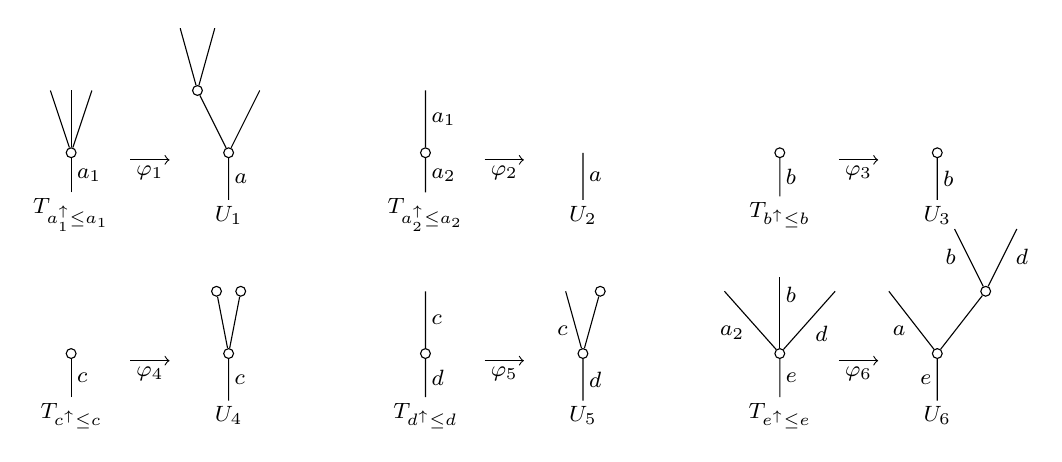
\begin{tikzpicture}[grow=up,auto,level distance=2.25em,
	every node/.style = {font=\footnotesize, inner sep=2pt},
	dummy/.style={circle,draw,inner sep=0pt,minimum size=1.25mm}]
	\begin{scope}
	\tikzstyle{level 2}=[sibling distance=0.75em]%
		\node at (0,0) {$T_{a_1^{\uparrow}\leq a_1}$}
			child{node [dummy] {}
				child
				child
				child
			edge from parent node [swap] {$a_1$}};
	\end{scope}	
	\begin{scope}
	\tikzstyle{level 2}=[sibling distance=2.25em]%
	\tikzstyle{level 3}=[sibling distance=1.25em]%
		\node at (2,0) {$U_1$}
			child{node [dummy] {}
				child
				child{node [dummy] {}
					child
					child
				}
			edge from parent node [swap] {$a$}};
	\end{scope}
		\draw [->] (0.75,0.7) -- node [swap]{$\varphi_1$} (1.25,0.7);
		\node at (4.5,0) {$T_{a_2^{\uparrow}\leq a_2}$}
			child{node [dummy] {}
				child{
				edge from parent node [swap] {$a_1$}}
			edge from parent node [swap] {$a_2$}};
		\node at (6.5,0) {$U_2$}
			child{
			edge from parent node [swap] {$a$}};
		\draw [->] (5.25,0.7) -- node [swap]{$\varphi_2$} (5.75,0.7);
		\node at (9,0) {$T_{b^{\uparrow}\leq b}$}
			child{node [dummy] {}
			edge from parent node [swap] {$b$}};
		\node at (11,0) {$U_3$}
			child{node [dummy] {}
			edge from parent node [swap] {$b$}};
		\draw [->] (9.75,0.7) -- node [swap]{$\varphi_3$} (10.25,0.7);
	\begin{scope}[yshift=-2.55cm]
		\node at (0,0) {$T_{c^{\uparrow}\leq c}$}
			child{node [dummy] {}
			edge from parent node [swap] {$c$}};
	\begin{scope}
	\tikzstyle{level 2}=[sibling distance=0.875em]%
		\node at (2,0) {$U_4$}
			child{node [dummy] {}
				child{node [dummy] {}}
				child{node [dummy] {}}
			edge from parent node  [swap]{$c$}};
	\end{scope}
	\draw [->] (0.75,0.7) -- node [swap]{$\varphi_4$} (1.25,0.7);
		\node at (4.5,0) {$T_{d^{\uparrow}\leq d}$}
			child{node [dummy] {}
				child{
				edge from parent node [swap] {$c$}}
			edge from parent node [swap] {$d$}};
	\begin{scope}
	\tikzstyle{level 2}=[sibling distance=1.25em]%
		\node at (6.5,0) {$U_5$}
			child{node [dummy] {}
				child{node[dummy] {}}
				child{
				edge from parent node {$c$}}
			edge from parent node [swap] {$d$}};
	\end{scope}
	\draw [->] (5.25,0.7) -- node [swap]{$\varphi_5$} (5.75,0.7);
	\begin{scope}
	\tikzstyle{level 2}=[sibling distance=2em]%
		\node at (9,0) {$T_{e^{\uparrow}\leq e}$}
			child{node [dummy] {}
				child{ edge from parent node [swap] {$d$} }
				child[level distance=2.75em]{ edge from parent node [near end,swap] {$b$} }
				child{ edge from parent node {$a_2$} }
			edge from parent node [swap] {$e$}};
	\end{scope}
	\begin{scope}
	\tikzstyle{level 2}=[sibling distance=3.5em]%
	\tikzstyle{level 3}=[sibling distance=2.25em]%
		\node at (11,0) {$U_6$}
			child{node [dummy] {}
				child{node [dummy] {}
					child{ edge from parent node [swap,near end] {$d$} }
					child{ edge from parent node [near end]{$b$} }
				}
				child{ edge from parent node {$a$} }
			edge from parent node {$e$}};
	\end{scope}
	\draw [->] (9.75,0.7) -- node [swap]{$\varphi_6$} (10.25,0.7);
	\end{scope}
	\end{tikzpicture}
\end{equation}
From this perspective, $U$ can now be thought as obtained from $T$ by substituting each of its nodes with the corresponding $U_i$. Moreover, the $\varphi_i$ assemble to a planar tall map 
$\varphi \colon T \to U$ (such that $a_i \mapsto a,b \mapsto b,\cdots,e \mapsto e$), which likewise encodes the same information.

Our perspective will then be that data for substitution of tree nodes such as in (\ref{SUBSDATUMTREES2 EQ}) can equivalently be 
repackaged using planar tall maps. 
\end{example}


\begin{definition}\label{SUBSTITUTIONDATUM}
	Let $T \in \Omega$ be a tree.
	
	A \textit{$T$-substitution datum} is a tuple 
	$\{U_{e^{\uparrow} \leq e}\}_{(e^{\uparrow} \leq e)\in V(T)}$ together with tall maps
	$T_{e^{\uparrow}\leq e} \to U_{e^{\uparrow}\leq e}$.
	
	Further, a map of $T$-substitution data 
	$\{U_{e^{\uparrow} \leq e}\} \to \{V_{e^{\uparrow} \leq e}\}$ is a tuple of tall maps $\{U_{e^{\uparrow} \leq e}\to V_{e^{\uparrow} \leq e}\}$ compatible with the chosen maps.
	
	Lastly, a substitution datum is called a $\textit{planar $T$-substitution datum}$ if the chosen maps are planar (so that 
	$\mathsf{lr}(U_{e^{\uparrow} \leq e}) = T_{e^{\uparrow} \leq e}$) and a morphism of planar data is called a planar morphism if it consists of a tuple of planar maps.
\end{definition}

\begin{definition}
	Let $T \in \Omega$. 
	
	The \textit{Segal core poset $\mathsf{Sc}(T)$} is the poset with objects the edge subtrees $\eta_e$ and vertex substrees $T_{e^{\uparrow} \leq e}$. The order relation is given by inclusion.
\end{definition}

\begin{remark}
Note that the only maps in $\mathsf{Sc}(T)$ are inclusions of the form $\eta_a \subset T_{e^{\uparrow}\leq e}$.
In particular, there are no pairs of composable non-identity relations in $\mathsf{Sc}(T)$. 
\end{remark}

Given a $T$-substitution datum $\{U_{\{e^{\uparrow}\leq e\}}\}$ we abuse notation by writing
\[U_{(\minus)} \colon \mathsf{Sc}(T) \to \Omega\]
for the functor $\eta_a \mapsto \eta$, $T_{e^{\uparrow} \leq e} \mapsto U_{e^{\uparrow} \leq e}$  
and sending the inclusions $\eta_a \subset T_{e^{\uparrow} \leq e}$
to the composites
\[
\eta \xrightarrow{a} T_{e^{\uparrow} \leq e}  \to 
%\simeq 
%\mathsf{lr}(U_{e^{\uparrow}\leq e}) \to 
U_{e^{\uparrow} \leq e}.\]


\begin{proposition}\label{SUBDATAUNDERPLAN PROP}
Let $T \in \Omega$ be a tree. There is an isomorphism of categories
\begin{equation}\label{SUBDATAUNDERPLAN EQ}
\begin{tikzcd}[row sep =0pt]
	\mathsf{Sub}_p(T) \ar[r,shift left=2pt] &
	\Omega_{T/}^{\mathsf{pt}} \ar[l,shift left=2pt]
\\
	\{U_{e^{\uparrow} \leq e}\} \ar[r,mapsto] & 
	\left(T \to \colim_{\mathsf{Sc}(T)} U_{(\minus)}\right)
\\
	\{U_{\varphi(e^{\uparrow}) \leq \varphi(e)}\} &
	(T \xrightarrow{\varphi} U) \ar[l,mapsto]
\end{tikzcd}
\end{equation}
where $\mathsf{Sub}_p(T)$ denotes the category of planar $T$-substitution data and $\Omega_{T/}^{\mathsf{pt}}$
the category of planar tall maps under $T$. 
\end{proposition}

\begin{proof}
We first claim that
\begin{inparaenum}
\item[(i)] the $\colim_{\mathsf{Sc}(T)} U_{(\minus)}$ indeed exists;
\item[(ii)] for the canonical datum $\{T_{e^{\uparrow}\leq e}\}$, it is $T = \colim_{\mathsf{Sc}(T)} T_{(\minus)}$;
\item[(iii)] the induced map
$T \to \colim_{\mathsf{Sc}(T)} U_{(\minus)}$ is planar tall.
\end{inparaenum}
 
The argument is by induction on the number of vertices of $T$, with the base cases of $T$ with $0$ or $1$ vertices being immediate, since then $T$ is the terminal object of $\mathsf{Sc}(T)$.
Otherwise, one can choose a non trivial grafting decomposition so as to write $T = R \amalg_e S$, resulting 
in identifications 
$\mathsf{Sc}(R) \subset \mathsf{Sc}(T)$, 
$\mathsf{Sc}(S) \subset \mathsf{Sc}(T)$
so that 
$\mathsf{Sc}(R) \cup \mathsf{Sc}(S) = \mathsf{Sc}(T)$
and 
$\mathsf{Sc}(R) \cap \mathsf{Sc}(S) = \{\eta_e \}$.
The existence of $\colim_{\mathsf{Sc}(T)}U_{(\minus)}$
is thus equivalent to the existence of the pushout below.
\begin{equation}\label{ASSEMBLYGRAFT EQ}
\begin{tikzcd}
	\eta \ar{r} \ar{d} & \colim_{\mathsf{Sc}(R)}U_{(\minus)} \ar[dashed,d]
\\
	\colim_{\mathsf{Sc}(S)}U_{(\minus)} \ar[dashed,r] &
	\colim_{\mathsf{Sc}(T)}U_{(\minus)}
\end{tikzcd}
\end{equation}
By induction, the top right and bottom left colimits exist for any $U_{(\minus)}$, 
equal $R$ and $S$ in the case $U_{(\minus)} = T_{(\minus)}$,
and the maps 
$R \to \colim_{\mathsf{Sc}(R)}U_{(\minus)}$,
$S \to \colim_{\mathsf{Sc}(S)}U_{(\minus)}$
are planar tall.
But it now follows that (\ref{ASSEMBLYGRAFT EQ}) is a grafting pushout diagram (cf. (\ref{GRAPTPUSH EQ})), so that the pushout indeed exists. The conditions that
$T = \colim_{\mathsf{Sc}(T)}T_{(\minus)}$
and 
$T \to \colim_{\mathsf{Sc}(T)}U_{(\minus)}$
is planar tall follow.

The fact that the two functors in (\ref{SUBDATAUNDERPLAN EQ})
are inverse to each other is clear by the same inductive argument.
\end{proof}


\begin{corollary}\label{SUBDATAUNDERPLAN COR}
Let $T \in \Omega$ be a tree. There is an isomorphism of categories
\begin{equation}\label{SUBDATAUNDERNONPL EQ}
\begin{tikzcd}[row sep =0pt]
	\mathsf{Sub}(T) \ar[r,shift left=2pt] &
	\Omega_{T/}^{\mathsf{t}} \ar[l,shift left=2pt]
\end{tikzcd}
\end{equation}
where $\mathsf{Sub}(T)$ denotes the category of $T$-substitution data and $\Omega_{T/}^{\mathsf{t}}$
the category of tall maps under $T$.
\end{corollary}


\begin{proof}
	This is a consequence of Proposition \ref{PLANARPULL EQ} together with the previous result, with the functor 
	$\mathsf{Sub}(T) \to \Omega_{T/}^{\mathsf{t}}$ given by the same formula.
	Indeed, Proposition \ref{PLANARIZATIONCHAR PROP} can be restated as saying that isomorphisms $T \to T'$ are in bijection with substitution data consisting of isomorphisms, and thus  bijectiveness reduces to that in the previous result.
\end{proof}


\begin{remark}\label{VERTEXDECOMP REM}
	It follows from the previous proof that, writing 
	$U = \colim_{\mathsf{Sc}(T)}U_{(\minus)}$,
	one has 
\begin{equation}\label{VERTEXDECOMP EQ}
	V(U) = \coprod_{(e^{\uparrow} \leq e) \in V(T)}
	V(U_{e^{\uparrow} \leq e}).
\end{equation}
Alternatively, (\ref{VERTEXDECOMP EQ}) can be regarded as a map 
$f^{\**} \colon V(U) \to V(T)$ induced by the planar tall map 
$f \colon T \to U$.
Explicitly, $f^{\**}(U_{u^{\uparrow} \leq u})$ 
is the unique $T_{t^{\uparrow}\leq t}$ such that
$U_{u^{\uparrow} \leq u} \subset U_{t^{\uparrow} \leq t}$. We note that $f^{\**}$ is indeed contravariant in the tall planar map $f$.
\end{remark}


The following is a converse of sorts to
 Proposition \ref{SUBDATAUNDERPLAN PROP}.

\begin{proposition}\label{BUILDABLE PROP}
	Let $U \in \Omega$ be a tree. Then:
\begin{itemize}
	\item[(i)] given non stick outer subtrees $U_i$ such that 
	$V(U) = \coprod_i V(U_i)$ there is a unique tree $T$ and planar tall map $T \to U$ such that $\{U_i\} = \{U_{e^{\uparrow}\leq e}\}$;
	\item[(ii)] given multiplicities $m_e \geq 1$ for each edge $e \in U$, there is a unique planar degeneracy $\rho \colon T \to U$ such that $\rho^{-1}(e)$ has $m_e$ elements;
	\item[(iii)] planar tall maps $T \to U$ are in bijection with collections $\{U_i\}$ of outer subtrees such that $V(U) = \coprod_i V(U_i)$ and $U_j$ is not an inner edge of any $U_i$ whenever $U_j \simeq \eta$ is a stick.
\end{itemize}
\end{proposition}


\begin{proof}
	We first show (i) by induction on the number of subtrees $U_i$. The base case $\{U_i\}=\{U\}$ is immediate, setting 
	$T= \mathsf{lr}(U)$. Otherwise, letting $e$ be edge that is both an inner edge of $U$ and a root of some $U_i$, and one can form a pushout diagram
\begin{equation} \label{DECOMPPROOF EQ}
\begin{tikzcd}
	\eta \ar{r}{e} \ar{d}[swap]{e} & V \ar{d}
\\
	W \ar{r} & U
\end{tikzcd}
\end{equation}
inducing a nontrivial partition 
$\{U_i\} = \{U_i|U_i \hookrightarrow V\} 
\amalg \{U_i|U_i \hookrightarrow W\}$. Existence of $T \to U$ now follows from the induction hypothesis. For uniqueness, the condition that no $U_i$ is a stick guarantees that $T$ possesses a single inner edge mapping to $e$, and thus admits a compatible decomposition as in (\ref{DECOMPPROOF EQ}), and thus uniqueness too follows by the induction hypothesis.

For (ii), we argue existence by nested induction on the number of vertices $|V(U)|$ and the sum of the multiplicities $m_e$. The base case $|V(U)|=0$, i.e., $U = \eta$ is immediate. Otherwise, writing $m_e = m'_e +1$, one can form a decomposition (\ref{DECOMPPROOF EQ}) where either $|V(V)|,|V(W)|<|V(U)|$ or one of $V,W$ is $\eta$, so that $T \to U$ can be built via the induction hypothesis. For uniqueness, note first that 
by \cite[Lemma 5.33]{Pe17} each pre-image $\rho^{-1}(e)$ is linearly ordered and by the ``further'' claim in 
\cite[Cor. 5.39]{Pe17} the remaining broad relations are precisely the pre-image of the non-identity relations in $U$, showing that the tree $T$ is uniquely determined.

(iii) follows by combining (i) and (ii). Indeed, any planar tall map $T \to U$ has a unique decomposition 
$T \twoheadrightarrow \bar{T} \hookrightarrow U$
as a planar degeneracy followed by a planar inner face, and each  of these maps is classified by the data in (b) and (a).
\end{proof}


\begin{lemma}\label{OUTERFACEUNION LEM}
	Suppose $T_1,T_2 \hookrightarrow T$ are two outer faces with at least one common edge $e$. Then there exists an unique outer face $T_1 \cup T_2$ such that 
	$V(T_1 \cup T_2) = V(T_1) \cup V(T_2)$.
\end{lemma}

\begin{proof}
	If either of $T_1,T_2$ is the root or a leaf the result is obvious. Otherwise, one can necessarily choose $e$ to be an inner edge of $T$, in which case all of $T_1,T_2,T$ admit compatible decompositions (\ref{DECOMPPROOF EQ}) and the result follows by induction on $|V(T)|$.
\end{proof}



\section{The genuine equivariant operad monad}\label{GENUINE_OP_MONAD_SECTION}
We now turn to the task of building the monad encoding genuine equivariant operads.



\subsection{Wreath product over finite sets}

In what follows we will let $\Fin$ denote the usual skeleton of the category of (ordered) finite sets and all set maps. Explicitly, its objects are the finite sets $\{1,2,\cdots,n\}$ for $n\geq 0$.
However, much as in the discussion in 
Convention \ref{PLANARCONV CON} we will often find it more convenient to regard the elements of $\Fin$ as equivalence classes of finite sets equipped with total orders.
 

\begin{definition}
	For a category $\C$, we let $\Fin \wr \C$ denote the opposite of the Grothendieck construction for the functor
\[
\begin{tikzcd}[row sep=0pt]
	\Fin^{op} \ar{r} & \mathsf{Cat}
\\
	I \ar[r,mapsto] & \C^I
\end{tikzcd}	
 \]
Explicitly, the objects of $\Fin \wr \C$ are tuples $(c_i)_{i \in I}$ and a map 
$(c_i)_{i \in I} \to (d_j)_{j \in J}$ consists of a pair 
\[(\phi \colon I \to J, (f_i\colon c_i \to d_{\phi(i)})_{i\in I}),\]
 henceforth abbreviated as $(\phi,(f_i))$.
\end{definition}
 
 The following is immediate.

\begin{proposition}
	Suppose $\C$ has all finite coproducts. One then has a functor as on the left below.
Dually, if $\C$ has all finite products, one has a functor as on the right below.
\[
\begin{tikzcd}[row sep=0pt]
	\Fin \wr \C \ar{r}{\coprod} & \C & &
	(\Fin \wr \C^{op})^{op} \ar{r}{\prod} & \C
\\
	(c_i)_{i \in I} \ar[mapsto]{r} & \coprod_{i \in I}{c_i} & &
	(c_i)_{i \in I} \ar[mapsto]{r} & \prod_{i \in I}{c_i}
\end{tikzcd}
\]
\end{proposition}



\begin{lemma}\label{FINWREATPRODLIM LEM}
Suppose that $\mathcal{E}$ is a bicomplete category such that 
coproducts commute with limits in each variable. If the leftmost diagram
\begin{equation}\label{WRRAN EQ}
	\begin{tikzcd}
	\mathcal{C} \ar{r}[swap,name=F]{}{F} \ar{d}[swap]{k} &
	\mathcal{E} & 
	& 
	\Fin \wr \mathcal{C} \ar{r}[swap,name=FF]{}{\Fin \wr F} \ar{d}[swap]{\Fin \wr k}&
	\Fin \wr \mathcal{E} \ar{r}{\amalg} &
	\mathcal{E}
		\\
	|[alias=D]|\mathcal{D} \ar{ru}[swap]{G} &
	& & 
	|[alias=FD]|\Fin \wr \mathcal{D} \ar{ru}[swap]{\Fin \wr G}
	\ar[bend right=13]{rru}[swap]{\amalg \circ \Fin \wr G}
	\arrow[Rightarrow, from=D, to=F,shorten <=0.10cm,"\eta"]
	\arrow[Rightarrow, from=FD, to=FF,shorten <=0.10cm,"\Fin \wr \eta"]
	\end{tikzcd}
\end{equation}
is a right Kan extension diagram then so is the composite of the rightmost diagram. 

Dually, if in $\mathcal{E}$ products commute with colimits in each variable, and the leftmost diagram
\begin{equation}\label{WRLAN EQ}
	\begin{tikzcd}[column sep = 4.5em]
	\mathcal{C}^{op} \ar{r}[swap,name=F]{}{F} \ar{d}[swap]{k} & 
	\mathcal{E} & 
	(\Fin \wr \mathcal{C})^{op} \ar{d}[swap]{(\Fin \wr k^{op})^{op}} 
	\ar{r}[swap,name=FF]{}{(\Fin \wr F^{op})^{op}} & 
	(\Fin \wr \mathcal{E}^{op})^{op} \ar{r}{\Pi} &
	\mathcal{E}
	\\
	|[alias=D]|\mathcal{D}^{op} \ar{ru}[swap]{G} &
	& 
	|[alias=FD]|(\Fin \wr \mathcal{D})^{op} 
	\ar{ru}[swap]{(\Fin \wr G^{op})^{op}}
	\ar[bend right=13]{rru}[swap]{\Pi \circ (\Fin \wr G^{op})^{op}}
	&
	\arrow[Leftarrow, from=D, to=F,shorten <=0.10cm,"\epsilon"]
	\arrow[Leftarrow, from=FD, to=FF,shorten <=0.10cm]
	\end{tikzcd}
\end{equation}
is a left Kan extension diagram then so is the composite of the rightmost diagram. 
\end{lemma}


\begin{proof}
	Unpacking definitions using the pointwise formula for Kan extensions (\cite[X.3.1]{McL}), the claim concerning (\ref{WRRAN EQ}) amounts to showing that for each $(d_i) \in \Fin \wr \mathcal{D}$ one has natural isomorphisms
	\begin{equation}\label{POINTKAN EQ}
	\underset{((d_i) \to (kc_j))\in
	\left( (d_i) \downarrow \Fin \wr \C \right) }{\lim} {\left(\coprod_j{F(c_j)}\right)}
		\simeq	
	\coprod_i \underset{(d_i  \to kc_i) \in d_i \downarrow \C}{\lim}
	\left(F(c_i)\right).
	\end{equation}
But since the canonical factorizations of each $(\varphi,(f_i))\colon (d_i)_{i \in I} \to (k c_j)_{j \in J}$ as
\[(d_i)_{i\in I} \to (c_{\phi(i)})_{i \in I} \to (k c_j)_{j \in J}\]
exhibit $\prod_{i}{(d_i\downarrow \mathcal{C})}$ as a coreflexive subcategory of $(d_i)\downarrow \Fin \wr \mathcal{C}$, we conclude in particular that it is an initial subcategory. Therefore
	\[
	\underset{((d_i) \to (kc_j))\in
	\left( (d_i)\downarrow \Fin \wr \C \right) }{\lim} {\left(\coprod_j{F(c_j)}\right)}
		\simeq	
	\underset{((d_i) \to (kc_i))\in
	\prod_{i} \left( {d_i \downarrow \mathcal{D}} \right)}{\lim}
	\left(\coprod_i{F(c_i)}\right)
	\]
and hence the isomorphisms (\ref{POINTKAN EQ}) now follow from the assumption that coproducts commute with limits in each variable.
\end{proof}

\begin{notation}
Using the coproduct functor $\Fin^{\wr 2} = \Fin^{\wr \{{0,1\}}} =\Fin \wr \Fin \xrightarrow{\amalg} \Fin$ (where $\coprod_{i\in I} J_i$ is ordered lexicographically) and the simpleton $\{1\} \in \Fin$
one can regard the collection of categories 
$\Fin^{\wr \{0,\cdots,n\}} \wr \C = \Fin^{\wr \underline{n}} \wr \C$
 as a coaugmented cosimplicial object in $\mathsf{Cat}$.
As such, we will denote by
\[
	\delta^i\colon \Fin^{\wr \underline{n-1}} \wr \C \to \Fin^{\wr \underline{n}} \wr \C, \qquad 0 \leq i \leq n
\]
the cofaces obtained by inserting simpletons $\{1\} \in \Fin$ and by 
\[
	\sigma^i \colon \Fin^{\wr \underline{n+1}} \wr \C \to \Fin^{\wr \underline{n}} \wr \C, \qquad 0 \leq i \leq n
\]
the codegeneracies obtained by applying the coproduct 
$\Fin^{\wr 2} \xrightarrow{\amalg} \Fin$ to adjacent 
$\Fin$ coordinates.
\end{notation}



\subsection{Equivariant leaf-root and vertex functors}\label{LRVERT SEC}

\begin{definition}
	A morphism $T \xrightarrow{\varphi} S$ in $\Omega_G$ is called a \textit{quotient} if the underlying morphism of (non-planar) forests
	\[\coprod_{[g]\in G/H} {T_{[g]} } 
	\to
	\coprod_{[h]\in G/K} {S_{[h]} } 
	\]
maps each tree component (or, equivalently, some tree component) isomorphically onto its image component.

We denote the subcategory of $G$-trees and quotients by $\Omega_G^q$.
\end{definition}


\begin{definition}
	The \textit{$G$-symmetric category}, which we will also call the \textit{category of $G$-corollas}, is the full subcategory 
	$\Sigma_G \subset \Omega_G^{q}$ of those $G$-trees that are corollas, i.e. $G$-trees such that each edge is either a root or a leaf (but not both).
\end{definition}


\begin{definition}
	The \textit{leaf-root functor} is the functor $\Omega_G^q \xrightarrow{\mathsf{lr}} \Sigma_G$ defined by 
	\[
	 \mathsf{lr}(T)=\{\text{leaves of }T\}\amalg \{\text{roots of }T\}
	\]
	with a broad relation $l_1 \cdots l_n \leq r$ holding in 
	$\mathsf{lr}(T)$ iff its image holds in $T$ and similarly for the planar structure $\leq_p$.
\end{definition}

\begin{remark}\label{LEAFROOTEXAMP REM}
	Generalizing Remark \ref{UNIQCOR REM},
	$\mathsf{lr}(T)$ can alternatively be characterized as being the \textit{unique} $G$-corolla which admits an also unique (tree-wise) tall planar map $\mathsf{lr}(T) \to T$. Moreover, $\mathsf{lr}(T)$ can usually be regarded as the ``smallest inner face'' of $T$, obtained by removing all the inner edges, although this characterization fails when 
	$T=G\cdot_H \eta$ is a stick $G$-tree. Some examples with $G=\mathbb{Z}_{/4}$ follow.
\[
	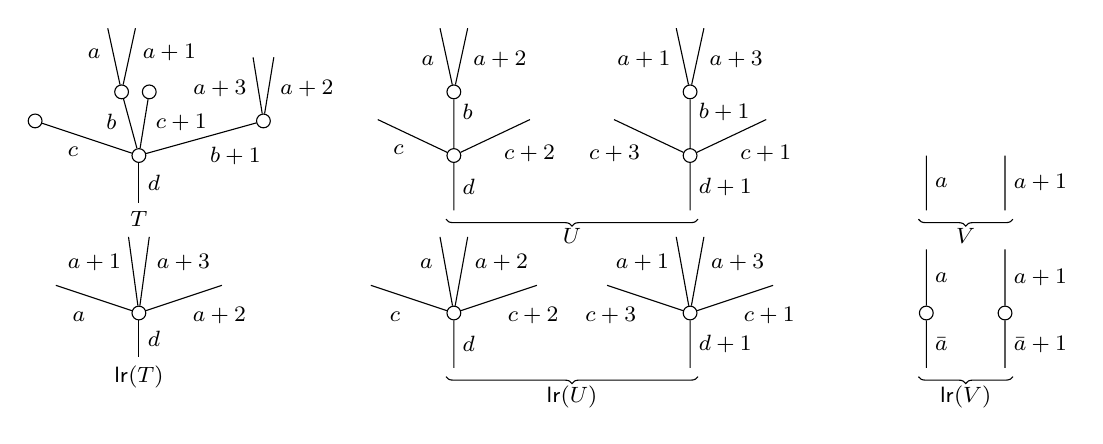
\begin{tikzpicture}[grow=up,auto,level distance=2.3em,
	every node/.style = {font=\footnotesize,inner sep=3pt},
	dummy/.style={circle,draw,inner sep=0pt,minimum size=1.75mm}]
		\node at (0,0) {$T$}
			child{node [dummy] {}
				child[level distance=1.25em,sibling distance = 3em]{node [dummy] {}
					child[level distance=2.3em,sibling distance =0.75em]{
					edge from parent node [swap,near end] {$a+2$}}
					child[level distance=2.3em,sibling distance =0.75em]{
					edge from parent node [near end] {$a+3$}}
				edge from parent node [swap] {$b+1$}}
				child[sibling distance = 0.75em]{node [dummy] {}
				edge from parent node [swap, very near end] {$c+1$}}
				child[sibling distance = 1.25em]{node [dummy] {}
					child[sibling distance = 1em]{
					edge from parent node [swap,very near end] {$a+1$}}
					child[sibling distance = 1em]{
					edge from parent node [very near end] {$\phantom{1+}a$}}
				edge from parent node [very near end] {$b$}}
				child[level distance=1.25em,sibling distance = 2.5em]{node [dummy] {}
				edge from parent node {$c$}}
			edge from parent node [swap] {$d$}};
		\node at (0,-2) {$\mathsf{lr}(T)$}
			child{node [dummy] {}
				child[sibling distance=2em, level distance=1em]{
				edge from parent node [swap] {$a+2$}}
				child[sibling distance=0.75em,level distance=2.75em]{
				edge from parent node [very near end,swap] {$a+3$}}
				child[sibling distance=0.75em,level distance=2.75em]{
				edge from parent node [very near end] {$a+1$}}
				child[sibling distance=2em, level distance=1em]{
				edge from parent node {$\phantom{1+}a$}}
			edge from parent node [swap] {$d$}};
		\node at (4,0) {}
			child{node [dummy] {}
				child[level distance=1.3em,sibling distance=2.75em]{
				edge from parent node [swap] {$c+2$}}
				child{node [dummy] {}
					child[sibling distance=1em]{
					edge from parent node [near end,swap] {$a+2$}}
					child[sibling distance=1em]{
					edge from parent node [near end] {$\phantom{1}a$}}
				edge from parent node [swap, near end] {$b$}}
				child[level distance=1.3em,sibling distance=2.75em]{
				edge from parent node {$c$}}
			edge from parent node [swap] {$d$}};
		\node at (7,0) {}
			child{node [dummy] {}
				child[level distance=1.3em,sibling distance=2.75em]{
				edge from parent node [swap] {$c+1$}}
				child{node [dummy] {}
					child[sibling distance=1em]{
					edge from parent node [near end,swap] {$a+3$}}
					child[sibling distance=1em]{
					edge from parent node [near end] {$a+1$}}
				edge from parent node [swap, near end] {$b+1$}}
				child[level distance=1.3em,sibling distance=2.75em]{
				edge from parent node {$c+3$}}
			edge from parent node [swap] {$d+1$}};
			\draw[decorate,decoration={brace,amplitude=2.5pt}] (7.1,0) -- (3.9,0) node[midway]{$U$};
		\node at (4,-2) {}
			child{node [dummy] {}
				child[sibling distance=2em, level distance=1em]{
				edge from parent node [swap] {$c+2$}}
				child[sibling distance=1em,level distance=2.75em]{
				edge from parent node [very near end,swap] {$a+2$}}
				child[sibling distance=1em,level distance=2.75em]{
				edge from parent node [very near end] {$\phantom{1+}a$}}
				child[sibling distance=2em, level distance=1em]{
				edge from parent node {$\phantom{1+}c$}}
			edge from parent node [swap] {$d$}};
		\node at (7,-2) {}
			child{node [dummy] {}
				child[sibling distance=2em, level distance=1em]{
				edge from parent node [swap] {$c+1$}}
				child[sibling distance=1em,level distance=2.75em]{
				edge from parent node [very near end,swap] {$a+3$}}
				child[sibling distance=1em,level distance=2.75em]{
				edge from parent node [very near end] {$a+1$}}
				child[sibling distance=2em, level distance=1em]{
				edge from parent node {$\phantom{1+}c+3$}}
			edge from parent node [swap] {$d+1$}};
			\draw[decorate,decoration={brace,amplitude=2.5pt}] (7.1,-2) -- (3.9,-2) node[midway]{$\mathsf{lr}(U)$};
			\node at (10,0) {}
				child{
				edge from parent node [swap] {$a$}};
			\node at (11,0) {}
				child{
				edge from parent node [swap] {$a+1$}};
			\draw[decorate,decoration={brace,amplitude=2.5pt}] (11.1,0) -- (9.9,0) node[midway]{$V$};
			\node at (10,-2) {}
				child{node[dummy]{}
					child{
					edge from parent node [swap] {$a$}}
				edge from parent node [swap] {$\bar{a}$}};
			\node at (11,-2) {}
				child{node[dummy]{}
					child{
					edge from parent node [swap] {$a+1$}}
				edge from parent node [swap] {$\bar{a}+1$}};
			\draw[decorate,decoration={brace,amplitude=2.5pt}] (11.1,-2) -- (9.9,-2) node[midway]{$\mathsf{lr}(V)$};
	\end{tikzpicture}
\]	
\end{remark}


\begin{remark}
	One consequence of the fact that planarizations can not be pushed forward along tree maps (cf. Remark \ref{PULLPLANAR REM})
is that $\mathsf{lr} \colon \Omega_G^q \to \Sigma_G$ is not a categorical fibration.
{\color{red} maybe add to this}.
\end{remark}


\begin{definition}\label{VG DEF}
	Given $T \in \Omega_G$ we define the set $V_G(T)$ of 
	\textit{$G$-vertices} of $T$ to be the orbit set $V(T)/G$, i.e. the quotient of the vertex set $V(T)$ by its $G$-action.
	
Furthermore, we will regard $V_G(T)$ as an object in $\Fin$ by equipping it with its lexicographic order: i.e. vertex equivalence classes $[e^{\uparrow} \leq e]$ are ordered according to the planar order $\leq_p$ of the smallest representative $ge$, $g \in G$.
\end{definition}



\begin{remark}\label{VERTEXDECOMPG REM}
	Following Remark \ref{VERTEXDECOMP REM},
	a planar tall map $f \colon T \to U$ of $G$-trees
	induces a $G$-equivariant map
	$f^{\**} \colon V(U) \to V(T)$
	and thus also a map of orbits
	$f^{\**} \colon V_G(U) \to V_G(T)$.
We note, however, that $f^{\**}$ is not in general compatible with the order on $V_G$, as is indeed the case even in the non-equivariant case.

A minimal example follows.
		\[
		\begin{tikzpicture}[grow=up,auto,level distance=2.4em,
		every node/.style = {font=\footnotesize},
		dummy/.style={circle,draw,inner sep=0pt,minimum size=1.75mm}]
		\node at (0,0) {$T$}
			child{node [dummy] {}
				child[sibling distance = 3.5em]{node [dummy] {}
					child
				edge from parent node[swap] {$c$}}
				child[level distance=2.9em]{
				edge from parent node [swap] {$b$}}
				child[sibling distance = 3.5em]{node [dummy] {}
					child
				edge from parent node {$a$}}		
			edge from parent node [swap] {$d$}};
		\node at (6,0) {$U$}
			child{node [dummy] {}
				child[sibling distance = 5em]{node [dummy] {}
					child
				edge from parent node [swap] {$c$}}
				child[sibling distance = 5em]{node [dummy] {}
					child[sibling distance = 3.5em]{
					edge from parent node [swap,near end] {$b$}}
					child[sibling distance = 3.5em]{node [dummy] {}
						child
					edge from parent node [near end]{$a$}}
				edge from parent node {$e$}}
			edge from parent node [swap] {$d$}};
		\draw[->] (2.6,1) -- node [above] {$f$} (3.6,1) ;
		\end{tikzpicture}
		\]
In $V(T)$ the vertices are ordered as $a<c<d$ while in $V(U)$ they are ordered as $a<e<c<d$ but the map 
$f^{\**} \colon V(U) \to V(T)$ is given by 
$a \mapsto a, c \mapsto c, d \mapsto d, e \mapsto d$.
\end{remark}


Note that each element of $V_G(T)$ corresponds to an unique edge orbit $Ge$ for $e$ not a leaf. As such, we will represent the corresponding $G$-vertex by $v_{Ge}=(Ge)^{\uparrow} \leq Ge$ (which we interpret as the concatenation of the relations $f^{\uparrow} \leq f$ for $f \in G e$) and write
\[T_{v_{Ge}}=T_{(Ge)^{\uparrow} \leq Ge} = \coprod_{f\in Ge} T_{f^{\uparrow}\leq f}.\]
We note that $T_{v_{Ge}}$ is always a $G$-corolla. Indeed, noting that a quotient map $\varphi \colon T \to S$ induces quotient maps 
$T_{v_{ge}} \to S_{v_{G\varphi(e)}}$ one obtains a functor
	\begin{equation}\label{VFUNCTOR EQ}
		\begin{tikzcd}[row sep=tiny]
		\Omega_G^q \ar{r}{V_G} & \Fin \wr \Sigma_G \\
		T \ar[mapsto]{r} & (T_{v_{Ge}})_{v_{Ge} \in V_G(T)}.
		\end{tikzcd}	
	\end{equation}

\begin{remark}
  \label{NEED_WREATH_REMARK}
	The need to introduce the $\Fin \wr \C$ categories comes from the fact that general quotient maps do not preserve the number of $G$-vertices. For a simple example, let $G=\mathbb{Z}_{/4}$ and consider the quotient map
		\[
		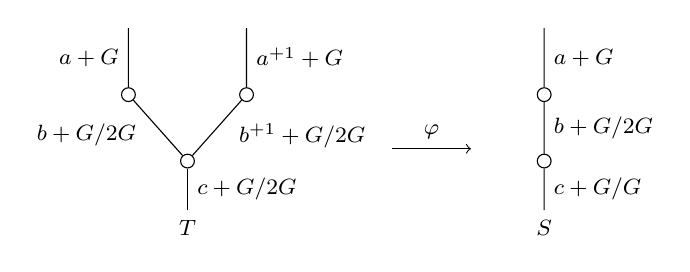
\begin{tikzpicture}[grow=up,auto,level distance=2.4em,every node/.style = {font=\footnotesize},dummy/.style={circle,draw,inner sep=0pt,minimum size=1.75mm}]
		\node at (0,0) {$T$}
			child{node [dummy] {}
				child{node [dummy] {}
					child{
					edge from parent node [swap] {$a^{+1} + G$}}
				edge from parent node[near end,swap] {$b^{+1} + G/2G$}}
				child{node [dummy] {}
					child{
					edge from parent node {$a + G$}}
				edge from parent node [near end] {$b + G/2G$}}		
			edge from parent node[swap] {$c + G/2G$}};
		\node at (4.53,0) {$S$}
			child{node [dummy] {}
				child{node [dummy] {}
					child{
					edge from parent node [swap] {$a + G$}}
				edge from parent node [swap] {$b + G/2G$}}
			edge from parent node [swap] {$c + G/G$}};
		\draw[->] (2.6,1) -- node [above] {$\varphi$} (3.6,1) ;
		\end{tikzpicture}
		\]
sending edges labeled $a,b,c$ to the edges with the same name and the edges $a^{+1}$, $b^{+1}$ to the edges $a+1$, $b+1$. We note that $T$ has three $G$-vertices $v_{Gc}$, $v_{Gb}$, $v_{Gb^{+1}}$ while $S$ has only two $G$-vertices $v_{Gc}$ and $v_{Gb}$. $V(\phi)$ then maps the two corollas 
$T_{v_{Gb}}$ and $T_{v_{G b^{+1}}}$
isomorphically onto $T_{S_{Gb}}$
and the corolla $T_{v_{Gc}}$ non-isomorphically onto $S_{v_{Gc}}$.
\end{remark}


Definition \ref{SUBSTITUTIONDATUM} now immediately generalizes. Here a map is called \textit{rooted} if it induces an ordered isomorphism on the root orbit.


\begin{definition}\label{SUBSTITUTIONDATUMG DEF}
	Let $T \in \Omega_G$ be a $G$-tree.
	
	A \textit{rooted (resp. planar) $T$-substitution datum} is a tuple 
	$\{U_{v_{G e}}\}_{v_{G e} \in V_G(T)}$ together with rooted (resp. planar) tall maps 
	$T_{v_{Ge}} \to U_{v_{G e}} = T_{v_{G e}}$.
	
	Further, a map of rooted (resp. planar) $T$-substitution data 
	$\{U_{v_{G e}}\} \to \{V_{v_{G e}}\}$ is a tuple of rooted (resp. planar) tall maps $\{U_{v_{G e}} \to V_{v_{G e}}\}$.
\end{definition}

\begin{remark}\label{SUBSDATUMCONV REM}
	To establish the equivariant analogue of Proposition \ref{SUBDATAUNDERPLAN PROP} we will prefer to repackage equivariant substitution data in terms of non-equivariant terms.

Noting that there are decompositions 
$U_{v_{G e}}= \coprod_{g e \in Ge} U_{ge^{\uparrow} \leq ge}$
and letting $G \ltimes V(T)$ denote the Grothendieck construction for the action of $G$ on the non-equivariant vertices $V(T)$ (often called the action groupoid), it is immediate that an equivariant $T$-substitution datum is the same as a functor $G \ltimes V(T) \to \Omega$ whose restriction to $V(T) \subset G \ltimes V(T)$ is a (non-equivariant) substitution datum.
\end{remark}


\begin{proposition}\label{SUBDATAUNDERPLANG PROP}
Let $T \in \Omega_G$ be a $G$-tree. There are isomorphisms of categories
\begin{equation}\label{SUBDATAUNDERPLANG EQ}
\begin{tikzcd}[row sep =0pt]
	\mathsf{Sub}_{\mathsf{p}}(T) \ar[r,shift left=2pt] &
	\Omega_{G,T/}^{\mathsf{pt}} \ar[l,shift left=2pt] &
	\mathsf{Sub}_{\mathsf{r}}(T) \ar[r,shift left=2pt] &
	\Omega_{G,T/}^{\mathsf{rt}} \ar[l,shift left=2pt]
\\
	\{U_{v_{G e}}\} \ar[r,mapsto] & 
	\left(T \to \colim_{\mathsf{Sc}(T)} U_{(\minus)}\right) &
	\{U_{v_{G e}}\} \ar[r,mapsto] & 
	\left(T \to \colim_{\mathsf{Sc}(T)} U_{(\minus)}\right)
\end{tikzcd}
\end{equation}
\end{proposition}


\begin{proof}
	This is a minor adaptation of the non-equivariant analogues Proposition \ref{SUBDATAUNDERPLANG PROP} and Corollary \ref{SUBDATAUNDERPLAN COR}.
	Since $\mathsf{Sc}(T)$ inherits a $G$ action, one can form the Grothendieck construction $G \ltimes \mathsf{Sc}(T)$ and by Remark \ref{SUBSDATUMCONV REM} equivariant substitution data $\{U_{v_{Ge}}\}$ therefore induce functors 
	$U_{(\minus)} \colon G \ltimes \mathsf{Sc}(T) \to \Omega$.
	It is then immediate that $\colim_{\mathsf{Sc}(T)} U_{(\minus)}$ inherits a $G$-action, provided it exists. 
	The key observation is then that, since $\mathsf{Sc}(T)$ is now a disconnected poset, this colimit is to be interpreted as taken in the category $\Phi$ of forests rather than in $\Omega$.
	
	Additionally, we note that the need to use rooted data comes from the fact that rooted isomorphisms $T \to T'$ are in bijection with rooted substitution data that are given by isomorphisms, a statement that fails in the absence of the rooted condition.
\end{proof}

\begin{remark} We will need to know that in the planar case each of the maps 
\[U_{v_{Ge}} \to U = \colim_{\mathsf{Sc}(T)}U_{(\minus)}\]
induced by the previous proof is a planar map of $G$-trees.
This requires two observations:
\begin{inparaenum}
	\item[(i)] the restrictions to each of the constituent non-equivariant trees $U_{ge^{\uparrow}\leq ge}$ is planar by Proposition \ref{SUBDATAUNDERPLANG PROP};
	\item[(ii)] the restriction to the roots of $U_{v_{Ge}}$ is injective and order preserving since it matches the inclusion of the roots of $T_{v_{Ge}}$, and the map $T \to U$ is a planar map of $G$-trees.
\end{inparaenum}
\end{remark}

\begin{remark}\label{PULLCOMP REM}
	The isomorphisms in Proposition \ref{SUBDATAUNDERPLANG PROP}
	are compatible with root pullbacks of trees. More concretely, any pullback $\pi \colon S=\varphi^{\**} T \to T$ induces pullbacks 
	$\pi_{Ge}\colon S_{v_{Ge}} \to T_{v_{Ge}}$ for $v_{Ge} \in V_G(S)$ and one has commutative diagrams
\begin{equation}\label{SUBDATAUNDERPLANG2 EQ}
\begin{tikzcd}[row sep =10pt]
	\mathsf{Sub}_{\mathsf{p}}(S) \ar[r,shift left=2pt] &
	\Omega_{G,S/}^{\mathsf{pt}} \ar[l,shift left=2pt] &
	\mathsf{Sub}_{\mathsf{r}}(S) \ar[r,shift left=2pt] &
	\Omega_{G,S/}^{\mathsf{rt}} \ar[l,shift left=2pt]
\\
	\mathsf{Sub}_{\mathsf{p}}(T) \ar[r,shift left=2pt] \ar{u}{(\pi_{Ge})} &
	\Omega_{G,T/}^{\mathsf{pt}} \ar[l,shift left=2pt] \ar{u}[swap]{\pi^{\**}} &
	\mathsf{Sub}_{\mathsf{r}}(T) \ar[r,shift left=2pt] \ar{u}{(\pi_{Ge})} &
	\Omega_{G,T/}^{\mathsf{rt}} \ar[l,shift left=2pt] \ar{u}[swap]{\pi^{\**}}
\end{tikzcd}
\end{equation}
\end{remark}



\subsection{Planar strings}\label{PLANARSTRING SEC}

The leaf-root and vertex functors will allow us to reinterpret our results concerning substitution.

\begin{definition}
	The category $\Omega_{G,n}$ of 
	\textit{substitution $n$-strings} is the category whose objects are strings
	\[
	\begin{tikzcd}
	T_0 \ar{r}{f_1} & T_1 \ar{r}{f_2} & \cdots \ar{r}{f_n} & T_n
	\end{tikzcd}	
	\]
	where $T_i \in \Omega_G$ and the $f_i$ are tall planar maps, and arrows are commutative diagrams 
	\begin{equation} \label{PTNARROW EQ}
	\begin{tikzcd}
	T_0 \ar{r}{f_1} \ar{d}[swap]{q_0} & T_1 \ar{r}{f_2} \ar{d}[swap]{q_1} & \cdots \ar{r}{f_n} & T_n \ar{d}[swap]{q_n}
\\
	T'_0 \ar{r}[swap]{f'_1} & T'_1 \ar{r}[swap]{f'_2} & \cdots \ar{r}[swap]{f'_n} & T'_n
	\end{tikzcd}	
	\end{equation}
where each $q_i$ is a quotient map.
\end{definition}


\begin{notation}\label{SIMPOPERATORS NOT}
	Since compositions of planar tall arrows are planar tall
	and identity arrows are planar tall	
	it follows that 
	$\Omega_{G,\bullet}$
	forms a simplicial object in $\mathsf{Cat}$, 
	with faces given by composing and degeneracies by inserting identities. 

	Noting that $\Omega_{G,0} = \Omega_G^q$ and setting 
	$\Omega_{G,-1} = \Sigma_G$, the leaf-root functor $\Omega_G^q \xrightarrow{\mathsf{lr}} \Sigma_G$ makes 
	$\Omega_{G,\bullet}^q$ into an augmented simplicial object and, furthermore, the maps 
	$s_{-1} \colon \Omega_{G,n}^q \to \Omega_{G,n+1}^q$
sending $T_0 \to T_1 \to \cdots \to T_n$ to 
$\mathsf{lr}(T_0) \to T_0 \to T_1 \to \cdots \to T_n$ equip it with extra degeneracies.
\end{notation}


\begin{notation}
We extend the vertex functor to a functor 
$V_G \colon \Omega_{G,n+1} \to \Fin \wr \Omega_{G,n}$
by
\begin{equation}\label{VGDEF EQ}
	V_G(T_0 \to T_1 \to \cdots \to T_n) = 
	(T_{1,v_{Ge}} \to \cdots \to
	T_{n,v_{Ge}})_{v_{Ge} \in V_G(T_0)}	
\end{equation}
where we abuse notation by writing $T_{i,v_{Ge}}$
for $T_{i, (f_i\circ \cdots \circ f_1)(v_{Ge})}$.
\end{notation}


The following is a reinterpretation of Proposition \ref{SUBDATAUNDERPLANG PROP}.

\begin{proposition} \label{SUBSASPULL PROP}
The diagram
	\begin{equation}\label{PTPULL EQ}
	\begin{tikzcd}
		\Omega_{G,n+1} \ar{r}{V_G} 
		\ar{d}[swap]{d_{1,\cdots,n+1}} & \Fin \wr \Omega_{G,n} 
		\ar{d}{\Fin \wr d_{0,\cdots,n}}
	\\
		\Omega_{G,0} \ar{r}[swap]{V_G} & \Fin \wr \Sigma_G
	\end{tikzcd}
	\end{equation}
is a pullback diagram in $\mathsf{Cat}$.
\end{proposition}


\begin{proof}
	An object in the pullback (\ref{PTPULL EQ}) over 
	$T\in \Omega_{G,0} = \Omega_G^q$ is precisely the same as a $n$-string in $\mathsf{Sub}(T)$, and thus by Proposition \ref{SUBDATAUNDERPLANG PROP} equivalent to a $n+1$ planar tall string starting at $T$.
	
	The case of arrows is slightly more subtle. A quotient map $\pi \colon T \to T'$ induces a $G$-equivariant poset map 
	$\pi_{\**} \colon \mathsf{Sc}(T) \to \mathsf{Sc}(T')$ 
	(or equivalently, a map of Grothendieck constructions 
	$G \ltimes \mathsf{Sc}(T) \to G \ltimes \mathsf{Sc}(T')$)
	and diagrams as on the left below (where $v_{Ge}$ ranges over $V_G(T)$ and $e'=\varphi(e)$) induce diagrams (of functors $\mathsf{Sc}(T) \to \Omega$) as on the right below.
	\begin{equation} \label{PTNARROWLOC EQ}
	\begin{tikzcd}[column sep=1.2em]
	T_{v_{G e}} \ar{r}{} \ar{d}[swap]{} & 
	T_{1,v_{G e}} \ar{r}{} \ar{d}[swap]{} &
	\cdots \ar{r}{} &
	T_{n,v_{G e}} \ar{d}{} &
	T_{(\minus)} \ar{r}{} \ar{d}[swap]{} & 
	T_{1,(\minus)} \ar{r}{} \ar{d}[swap]{} &
	\cdots \ar{r}{} &
	T_{n,(\minus)} \ar{d}{} &
\\
	T'_{v_{G e'}} \ar{r}{} &
	T'_{1,v_{G e'}} \ar{r}{} &
	\cdots \ar{r}{} &
	T'_{n,v_{G e'}} &
	T'_{(\minus)}\circ \pi_{\**} \ar{r}{} &
	T'_{1,(\minus)}\circ \pi_{\**} \ar{r}{} &
	\cdots \ar{r}{} &
	T'_{n,(\minus)}\circ \pi_{\**} &
	\end{tikzcd}	
	\end{equation}
Passing to colimits then gives the desired commutative diagram (\ref{PTNARROW EQ}). Moreover, diagrams of the form (\ref{PTNARROW EQ}) clearly induce diagrams as in  (\ref{PTNARROWLOC EQ}) and it is straightforward to check that these are inverse processes. 
\end{proof}


\begin{remark}\label{DSCOM REM}
The diagrams (with back and lower slanted faces instances of (\ref{PTPULL EQ}))
	\[
	\begin{tikzcd}[column sep = 0.1em]
		\Omega_{G,{n+2}} \ar{rr} \ar{rd}{d_{i+1}} \ar{dd}
		 & & \Fin \wr \Omega_{G,{n+1}} \ar{rd}{\Fin \wr d_i} \ar{dd} & &
		\Omega_{G,{n+1}} \ar{rr} \ar{rd}{s_{i}} \ar{dd} 
		& & \Fin \wr \Omega_{G,{n}} \ar{rd}{\Fin \wr s_{i-1}} \ar{dd} &
	\\
		& \Omega_{G,{n+1}} \ar{ld} \ar[crossing over]{rr} 
		& & \Fin \wr \Omega_{G,{n}} \ar{ld} &
		& \Omega_{G,{n+2}} \ar{ld} \ar[crossing over]{rr} 
		& & \Fin \wr \Omega_{G,{n+1}} \ar{ld}
	\\
		 \Omega_{G,0} \ar{rr} & & \Fin \wr \Sigma_G & &
		 \Omega_{G,0} \ar{rr} & & \Fin \wr \Sigma_G &
	\end{tikzcd}
	\]
commute whenever defined (i.e. $0 \leq i \leq n+1$).
\end{remark}


\begin{notation}\label{INDVNG NOT}
	We will let 
\[
	V_{G,n} \colon \Omega_{G,n} \to \Fin \wr \Sigma_G
\]
be inductively defined by 
$V_{G,n} = \sigma^0 \circ V_{G,n-1} \circ V_G$.
\end{notation}

\begin{remark}
When $n = 2$, $V_{G,2}$ is thus the composite
\[
\begin{tikzcd}[column sep =1.7em]
	\Omega_{G,2} \ar{r}{V_G} &
	\Fin \wr \Omega_{G,1} \ar{r}{V_G} &
	\Fin \wr \Fin \wr \Omega_{G,0} \ar{r}{V_G} &
	\Fin \wr \Fin \wr \Fin \wr \Sigma_{G} \ar{r}{\sigma^0} &
	\Fin \wr \Fin \wr \Sigma_{G} \ar{r}{\sigma^0} &
	\Fin \wr \Sigma_{G}
\end{tikzcd}
\]
In light of Remarks \ref{VERTEXDECOMP REM} and \ref{VERTEXDECOMPG REM}, 
$V_{G,n}(T_0 \to \cdots \to T_n)$ is identified with the tuple 
\begin{equation}\label{VGNISO EQ}
	(T_{n,v_{G e}})_{v_{G e} \in V_G(T_n)},
\end{equation}
though this requires changing the total order in $V_G(T_n)$. Rather than using the order induced by $T_n$, one instead equips 
$V_G(T_n)$ with the order induced lexicographically
from the maps 
$V_G(T_n) \to V_G(T_{n-1}) \to \cdots \to V_G(T_0)$, i.e., for 
$v,w \in V_G(T_n)$ the condition $v<w$ is determined by the lowest $i$ such that the images of $v,w \in V_G(T_i)$ are distinct.
\end{remark}




\subsection{A monad on spans}

\begin{definition}\label{WSPAN DEF}
We will write 
$\mathsf{WSpan}^l(\C,\D)$
(resp.
$\mathsf{WSpan}^r(\C,\D)$),
which we call the category of  \textit{left weak spans} (resp. \textit{right weak spans}),
to denote the category with objects the spans
\[
\begin{tikzcd}
\C & A \ar{l}[swap]{k} \ar{r}{F} & \D,
\end{tikzcd}
\]
arrows the diagrams as on the left (resp. right) below \begin{equation}\label{TWISTEDARROWRIGHT EQ}
	\begin{tikzcd}[row sep=small]
	&
	A_1 \ar{dl}[swap,name=k1]{k_1} \ar{dr}[name=F11]{F_1} \ar{dd}[swap]{i} & &
	&
	A_1 \ar{dl}[swap,name=k1]{k_1} \ar{dr}[name=F1]{F_1} \ar{dd}[swap]{i} 
\\
	\C & & \D &
	\C & & \D 
\\
		& |[alias=G21]| A_2  \ar{ul}{k_2} \ar{ur}[swap]{F_2} & &
		& |[alias=G2]| A_2  \ar{ul}{k_2} \ar{ur}[swap]{F_2} &
		\arrow[Leftarrow, from=F1, to=G2,shorten >=0.25cm,shorten <=0.25cm,"\varphi"]
		\arrow[Rightarrow, from=F11, to=G21,shorten >=0.25cm,shorten <=0.25cm,"\varphi"]
	\end{tikzcd}
\end{equation}
which we write as $(i,\varphi) \colon (k_1,F_1) \to (k_2,F_2)$, and composition given in the obvious way.
\end{definition}


\begin{remark}
There are natural isomorphisms
\begin{equation}\label{LRSPANISO EQ}
\mathsf{WSpan}^r(\C,\D) \simeq \mathsf{WSpan}^l(\C^{op},\D^{op}).
\end{equation}
\end{remark}


\begin{remark}\label{RANLANADJ REM}
The terms \textit{left/right} are motivated by the existence of adjunctions (which are seen to be equivalent by using (\ref{LRSPANISO EQ}))
\[
	\mathsf{Lan} \colon
	\mathsf{WSpan}^l(\C, \D)
		\rightleftarrows
	\mathsf{Fun}(\C, \D)
	\colon \iota
\]
\[
	\iota \colon 
	\mathsf{Fun}(\C, \D)
		\rightleftarrows
	\mathsf{WSpan}^r(\C, \D)^{op}
	\colon \mathsf{Ran}
\]
where the functors $\iota$ denote the obvious inclusions 
(note the need for the $(\minus)^{op}$ in the second adjunction) 
and $\mathsf{Lan}$/$\mathsf{Ran}$ denote the left/right Kan extension functors.
\end{remark}


We will mainly be interested in the span categories 
$\mathsf{WSpan}^l(\Sigma_G^{op},\mathcal{V})\simeq 
\mathsf{WSpan}^r(\Sigma_G,\mathcal{V}^{op})$.


\begin{notation}\label{OMEGAGNA NOT}
	Given a functor $\pi \colon A \to \Sigma_G$, we let $\Omega^{(A)}_{G,n}$ denote the pullback (in $\mathsf{Cat}$)
\[
	\begin{tikzcd}
	\Omega_{G,n}^{(A)} \ar{r}{V_{G,n}^{(A)}} \ar{d}& 
	\Fin \wr A \ar{d}
\\
	\Omega_{G,n} \ar{r}[swap]{V_{G,n}} &
	\Fin \wr \Sigma_G
	\end{tikzcd}
\]
Explicitly, the objects of $\Omega_{G,n}^{(A)}$ are pairs 
\begin{equation}\label{OMEGAGNA EQ}
(T_0 \to \cdots \to T_n,
(a_{e^{\uparrow} \leq e})_{(e^{\uparrow} \leq e)\in V_G(T_n)})
\end{equation}
such that $\pi(a_{e^{\uparrow} \leq e}) = T_{n,e^{\uparrow} \leq e}$.
\end{notation}

\begin{remark}
Our primary interest here will be in the 
$\Omega_{G,0}^{(A)}$ construction.
Importantly, the composite maps 
$\Omega_{G,0}^{(A)} \to \Omega_{G,0} \to \Sigma_G$
allow us to iterate the $\Omega_{G,0}^{(\minus)}$ construction. In practice, the role of higher strings $\Omega_{G,n}^{(A)}$ will then be to provide more convenient models for iterated 
$\Omega_{G,0}^{(\minus)}$ constructions.


Indeed, the content of Proposition \ref{SUBSASPULL PROP} is then that there are compatible identifications
$\Omega_{G,0}^{(\Omega_{G,n})} \simeq \Omega_{G,n+1}$
which identify $V_G^{(\Omega_{G,n})}$ with $V_G$.

Moreover, since all squares in the diagram
\begin{equation}\label{ALLSQUARES EQ}
\begin{tikzcd}
	\Omega^{(A)}_{G,n+1} \ar{r}{V_G^{(A)}} \ar{d}& 
	\Fin \wr \Omega^{(A)}_{G,n} \ar{r}{\Fin \wr V_{G,n}^{(A)}} \ar{d}&
	\Fin \wr \Fin \wr A  \ar{d} \ar{r}{\sigma^0} &
	\Fin \wr A \ar{d}
\\
	\Omega_{G,n+1} \ar{r}{V_G} \ar{d} &
	\Fin \wr \Omega_{G,n} \ar{r}{\Fin \wr V_{G,n}} \ar{d} &
	\Fin \wr \Fin \wr \Sigma_G \ar{r}{\sigma^0} &
	\Fin \wr \Sigma_G
\\
	\Omega_{G,0} \ar{r} &
	\Fin \wr \Sigma_G
\end{tikzcd}
\end{equation}
are pullback squares (the top center square is so by induction, the top right square by direct verification, the total top square by definition of $\Omega_{G,n+1}^{(A)}$ and the bottom left square by Proposition \ref{SUBSASPULL PROP}),
we likewise obtain identifications 
$\Omega_G^{\left(\Omega_{G,n}^{(A)}\right)} \simeq \Omega_{G,n+1}^{(A)}$.
\end{remark}


\begin{proposition}
For any $A \to \Sigma_G$ there are functors 
$d_0^{(A)}\colon \Omega_{G,1}^{(A)} \to \Omega_{G}^{(A)}$ and natural isomorphisms
\begin{equation}\label{SHUFFLEPERMA EQ}
	\begin{tikzcd}
	\Omega_{G,1}^{(A)} \ar{r}{V_G} \ar{d}[swap]{d_{0}^{(A)}}&
	\Fin \wr \Omega_{G}^{(A)} \ar{r}{\Fin \wr V_G} &
	|[alias=FFOmega]|\Fin \wr \Fin \wr A \ar{d}{\sigma^0}
\\
	|[alias=Omega]|\Omega_{G}^{(A)} \ar{rr}[swap]{V_G} &&
	\Fin \wr A,
	\arrow[Leftrightarrow, from=FFOmega, to=Omega,shorten <=0.15cm,,shorten >=0.15cm,"\pi^{(A)}"]
	\end{tikzcd}
\end{equation}
both natural in $A \to \Sigma$.
Here naturality of $\pi^{(\minus)}$ means that for a functor $H \colon A \to B$ with corresponding diagram
\begin{equation}\label{PICUBOIDAB EQ}
\begin{tikzcd}[column sep = small, row sep = small]
	\Omega_{G,1}^{(A)} \ar{rr}{V_G^{(A)}} \ar{rd}[swap,near end]{d^{(A)}_0} \ar{dd}[swap]{\Omega_{G,1}^{(H)}}
	&&
	\Fin \wr \Omega_{G,0}^{(A)} \ar{rr}{\Fin \wr V_G^{(A)}} \ar[dd,dashed]&&
	|[alias=FFOmegan]|\Fin \wr \Fin \wr A  \ar[dd,dashed] \ar{rd}{\sigma^0}
\\
	&
	|[alias=Omeganp1]|\Omega_{G,0}^{(A)} \ar[crossing over]{rrrr}[swap]{V_G^{(A)}} \ar[crossing over]{dd} &&&&
	\Fin \wr A \ar{dd}{\Fin \wr H}&
\\
	\Omega_{G,1}^{(B)} \ar[dashed]{rr} \ar{rd}[swap,near end]{d^{(B)}_0}&&
	\Fin \wr \Omega^{(B)}_{G,0} \ar[rr,dashed] &&
	|[alias=FFOmeganm1]|\Fin \wr \Fin \wr B \ar[rd,dashed] 
\\
	&
	|[alias=Omegan]|\Omega^{(B)}_{G,0} \ar{rrrr}[swap]{V_G^{(B)}} &&&&
	\Fin \wr B &
	\arrow[Leftrightarrow, from=Omeganp1, to=FFOmegan,shorten <=0.15cm,shorten >=0.15cm,swap,"\pi^{(A)}"]
	\arrow[Leftrightarrow, from=FFOmeganm1, to=Omegan,shorten <=0.15cm,shorten >=0.15cm,dashed]
\end{tikzcd}
\end{equation}
one has an equality 
\[(\Fin \wr H)\pi^{(A)} = \pi^{(B)}\Omega_{G,1}^{(H)}\]
 (i.e. the two natural isomorphisms between the two distinct functors $\Omega_{G,1}^{(A)} \rightrightarrows \Fin \wr B$ coincide).
\end{proposition}

\begin{proof}
Informally, using the object description in (\ref{OMEGAGNA EQ}),
$d_0^{(A)}$ is simply given by the formula
\begin{equation}\label{GEND0 EQ}
d_0^{(A)} \left(
T_0 \to T_1,
(a_{e^{\uparrow} \leq e})_{(e^{\uparrow} \leq e)\in V_G(T_1)}
\right)
=
\left(
T_1,
(a_{e^{\uparrow} \leq e})_{(e^{\uparrow} \leq e)\in V_G(T_1)}
\right),
\end{equation}
though one must note that since in (\ref{OMEGAGNA EQ}) the
order in $V_G(T_1)$ is induced lexicographically from the string, the two orders for $V_G(T_1)$ in each side of (\ref{GEND0 EQ})
do not coincide.

It now follows that the composites 
$\sigma^0 \circ (\Fin \wr V_G^{(A)}) \circ V_G^{(A)}$
and 
$V_G^{(A)} \circ d_0^{(A)}$
differ by the natural automorphism $\pi^{(A)}$
given by the tuple permutations interchanging the two orders in
$V_G(T_1)$ for each $T_0 \to T_1$.

The commutativity of (\ref{PICUBOIDAB EQ}) is clear.
\end{proof}


\begin{definition}
  \label{WSPAN_MONAD_DEFINITION}
	Suppose $\mathcal{V}$ has finite products.
	
	We define an endofunctor $N$ of 
	$\mathsf{Wspan}^r(\Sigma_G,\mathcal{V}^{op})$
	by letting $N(\Sigma_G \leftarrow A \to \mathcal{V}^{op})$
	be the span $\Sigma_G \leftarrow \Omega^{(A)}_{G,0} \to \mathcal{V}^{op}$ given composition along the diagram
\[
	\begin{tikzcd}
	\Omega^{(A)}_{G,0} \ar{r} \ar{d}&
	\Fin \wr A \ar{r} \ar{d}&
	\Fin \wr \mathcal{V}^{op} \ar{r}{\Pi^{op}} &
	\mathcal{V}^{op}
\\
	\Omega_{G,0} \ar{r} \ar{d} &
	\Fin \wr \Sigma_G
\\
	\Sigma_G
	\end{tikzcd}
\]
and defined on maps of spans in the obvious way.

One has a multiplication $\mu \colon N \circ N \Rightarrow N$ given by the natural isomorphisms
\begin{equation}\label{MULTDEFSPAN EQ}
	\begin{tikzcd}
	\Sigma \ar[equal]{d}&
	\Omega_{G,1}^{(A)} \ar{r}{V_G} \ar{d}[swap]{d_{0}^{(A)}} \ar{l}&
	\Fin \wr \Omega_{G,0}^{(A)} \ar{r}{\Fin \wr V_G} &
	|[alias=FFOmega]|\Fin \wr \Fin \wr A \ar{d}{\sigma^0} \ar{r} &
	\Fin \wr \Fin \wr \mathcal{V}^{op} \ar{d}{\sigma^0} \ar{r} &
	\Fin \wr \mathcal{V}^{op} \ar{r} &
	|[alias=dog]|
	\mathcal{V}^{op} \ar[equal]{d}
\\
	\Sigma &
	|[alias=Omega]|\Omega_{G,0}^{(A)} \ar{rr}[swap]{V_G} \ar{l}&&
	\Fin \wr A \ar{r} &
	|[alias=cat]|
	\Fin \wr \mathcal{V}^{op} \ar{rr} &&
	\mathcal{V}^{op}
	\arrow[Leftrightarrow, from=FFOmega, to=Omega,shorten <=0.15cm,,shorten >=0.15cm,"\pi^{(A)}"]
	\arrow[Leftrightarrow, from=dog, to=cat,shorten <=0.15cm,,shorten >=0.15cm,"\alpha"]
	\end{tikzcd}
\end{equation}
where $\alpha$ is an associativity isomorphism for the product $\Pi$. We we note that naturality of $\mu$ 
follows from the commutativity of (\ref{PICUBOIDAB EQ}).

Lastly, there is a unit $\eta \colon id \Rightarrow N$ given by the strictly commutative diagrams
\begin{equation}\label{UNITSPAN EQ}
	\begin{tikzcd}
	\Sigma \ar[equal]{d} &
	A \ar{l} \ar{d}[swap]{s_{-1}^{(A)}} \ar[equal]{r} &
	A \ar{d} \ar{r} &
	\mathcal{V}^{op} \ar{d} \ar[equal]{r}&
	\mathcal{V}^{op} \ar[equal]{d}
\\
	\Sigma &
	\Omega_{G,0}^{(A)} \ar{l} \ar{r}[swap]{V_G}&
	\Fin \wr A \ar{r} &
	\Fin \wr \mathcal{V}^{op} \ar{r} &
	\mathcal{V}^{op}.
	\end{tikzcd}
\end{equation}	
\end{definition}

\begin{proposition}\label{MONSPAN PROP}
$(N,\mu,\eta)$ form a monad on $\mathsf{Wspan}^r(\Sigma_G,\mathcal{V}^{op})$.
\end{proposition}

\begin{proof}
The natural transformation component of $\mu \circ (N \mu)$ is given by the composite diagram
\begin{equation}\label{ASSOCSPAN1 EQ}
	\begin{tikzcd}[column sep=1.05em]
	\Omega_{G,2}^{(A)}\ar{d}[swap]{d_1^{(A)}} \ar{r} &
	\Fin \wr \Omega_{G,1}^{(A)} \ar{d} \ar{r}&
	\Fin^{\wr 2} \wr \Omega_{G,0}^{(A)} \ar{r} &
	|[alias=dog2]|
	\Fin^{\wr 3} \wr A \ar{d}{\sigma^1} \ar{r} &
	\Fin^{\wr 3} \wr \mathcal{V}^{op} \ar{d}{\sigma^1} \ar{r} &
	\Fin^{\wr 2} \wr \mathcal{V}^{op} \ar{r}&
	|[alias=cat3]|
	\Fin \wr \mathcal{V}^{op} \ar[equal]{d} \ar{r} &
	\mathcal{V}^{op} \ar[equal]{d}
\\
	\Omega_{G,1}^{(A)} \ar{r} \ar{d}[swap]{d_{0}^{(A)}}&
	|[alias=cat2]|
	\Fin \wr \Omega_{G,0}^{(A)} \ar{rr} &&
	|[alias=FFOmega]|\Fin^{\wr 2} \wr A \ar{d}{\sigma^0} \ar{r} &
	|[alias=dog3]|
	\Fin^{\wr 2} \wr \mathcal{V}^{op} \ar{d}{\sigma^0} \ar{rr} &&
	\Fin \wr \mathcal{V}^{op} \ar{r} &
	|[alias=dog]|
	\mathcal{V}^{op} \ar[equal]{d}
\\
	|[alias=Omega]|\Omega_{G,0}^{(A)} \ar{rrr} &&&
	\Fin \wr A \ar{r} &
	|[alias=cat]|
	\Fin \wr \mathcal{V}^{op} \ar{rrr} &&&
	\mathcal{V}^{op}
	\arrow[Leftrightarrow, from=FFOmega, to=Omega,shorten <=0.15cm,shorten >=0.15cm,"\pi^{(A)}"]
	\arrow[Leftrightarrow, from=dog, to=cat,shorten <=0.15cm,shorten >=0.15cm,"\alpha"]
	\arrow[Leftrightarrow, from=dog2, to=cat2,shorten <=0.15cm,shorten >=0.15cm,"\Fin \wr \pi^{(A)}"]
	\arrow[Leftrightarrow, from=cat3, to=dog3,shorten <=0.15cm,shorten >=0.15cm,"\Fin \wr \alpha"]
	\end{tikzcd}
\end{equation}
whereas the natural transformation component of $\mu \circ (\mu N)$ is given by
\begin{equation}\label{ASSOCSPAN2 EQ}
	\begin{tikzcd}[column sep=1.05em]
	\Omega_{G,2}^{(A)} \ar{d}[swap]{d_0^{(A)}} \ar{r} &
	\Fin \wr \Omega_{G,1}^{(A)} \ar{r} &
	|[alias=dog2]|
	\Fin^{\wr 2} \wr \Omega_{G,0}^{(A)} \ar{r} \ar{d}&
	\Fin^{\wr 3} \wr A \ar{r} \ar{d}{\sigma^0} &
	\Fin^{\wr 3} \wr \mathcal{V}^{op} \ar{r} \ar{d}{\sigma^0} &
	\Fin^{\wr 2} \wr \mathcal{V}^{op} \ar{r} \ar{d}&
	\Fin^ \wr \mathcal{V}^{op} \ar{r} &
	|[alias=dog3]|
	\mathcal{V}^{op} \ar[equal]{d}
\\
	|[alias=cat2]|
	\Omega_{G,1}^{(A)} \ar{rr} \ar{d}[swap]{d_{0}^{(A)}} &&
	\Fin \wr \Omega_{G,0}^{(A)} \ar{r} &
	|[alias=FFOmega]|
	\Fin^{\wr 2} \wr A \ar{d}{\sigma^0} \ar{r} &
	\Fin^{\wr 2} \wr \mathcal{V}^{op} \ar{d}{\sigma^0} \ar{r} &
	|[alias=cat3]|
	\Fin \wr \mathcal{V}^{op} \ar{rr} &&
	|[alias=dog]|
	\mathcal{V}^{op} \ar[equal]{d}
\\
	|[alias=Omega]|\Omega_{G,0}^{(A)} \ar{rrr} &&&
	\Fin \wr A \ar{r} &
	|[alias=cat]|
	\Fin \wr \mathcal{V}^{op} \ar{rrr} &&&
	\mathcal{V}^{op}
	\arrow[Leftrightarrow, from=FFOmega, to=Omega,shorten <=0.15cm,,shorten >=0.15cm,"\pi^{(A)}"]
	\arrow[Leftrightarrow, from=dog, to=cat,shorten <=0.15cm,,shorten >=0.15cm,"\alpha"]
	\arrow[Leftrightarrow, from=dog2, to=cat2,shorten <=0.15cm,,shorten >=0.15cm,"\pi^{\left(\Omega_G^{(A)}\right)}"]
	\arrow[Leftrightarrow, from=dog3, to=cat3,shorten <=0.15cm,,shorten >=0.15cm,"\alpha"]
	\end{tikzcd}
\end{equation}

That the rightmost sections of (\ref{ASSOCSPAN1 EQ}) and (\ref{ASSOCSPAN2 EQ}) coincide follows from compatibility of the associativity isomorphisms for $\Pi^{op}$. 

For the leftmost sections, note first that, in either diagram,
the top right and bottom left paths $\Omega_{G,2}^{(A)} \to \Fin \wr A$ differ only by the induced order on $V_G(T_2)$ for each string $T_0 \to T_1 \to T_2$. More explicitly, the top right paths use the order induced lexicographically from the string $T_0 \to T_1 \to T_2$
while the bottom left paths use the order induced exclusively by $T_2$.
The two left sections then coincide since are both given by the permutation interchanging these orders, the only difference being that the intermediate stage of (\ref{ASSOCSPAN1 EQ}) uses the order induced lexicographically from $T_0 \to T_2$
while (\ref{ASSOCSPAN2 EQ}) uses the order induced lexicographically from $T_1 \to T_2$.

As for unit conditions, $\mu \circ (N \eta)$ is represented by
\begin{equation}\label{UNITSPAN1 EQ}
	\begin{tikzcd}[column sep=1.05em]
	\Omega_G^{(A)} \ar{d}[swap]{s_{0}^{(A)}} \ar{r} &
	\Fin \wr A \ar{d} \ar[equal]{r} &
	\Fin \wr A \ar{d}{\delta^1} \ar{r} &
	\Fin \wr \mathcal{V}^{op} \ar{d}{\delta^1} \ar[equal]{r} &
	\Fin \wr \mathcal{V}^{op} \ar[equal]{d} \ar{r} &
	\mathcal{V}^{op} \ar[equal]{d}
\\
	\Omega_{G,1}^{(A)} \ar{r} \ar{d}[swap]{d_{0}^{(A)}}&
	\Fin \wr \Omega_{G}^{(A)} \ar{r} &
	|[alias=FFOmega]|\Fin^{\wr 2} \wr A \ar{d}{\sigma^0} \ar{r} &
	\Fin^{\wr 2} \wr \mathcal{V}^{op} \ar{d}{\sigma^0} \ar{r} &
	\Fin \wr \mathcal{V}^{op} \ar{r} &
	|[alias=dog]|
	\mathcal{V}^{op} \ar[equal]{d}
\\
	|[alias=Omega]|\Omega_{G}^{(A)} \ar{rr}&&
	\Fin \wr A \ar{r} &
	|[alias=cat]|
	\Fin \wr \mathcal{V}^{op} \ar{rr} &&
	\mathcal{V}^{op}
	\arrow[Leftrightarrow, from=FFOmega, to=Omega,shorten <=0.15cm,,shorten >=0.15cm,"\pi^{(A)}"]
	\arrow[Leftrightarrow, from=dog, to=cat,shorten <=0.15cm,,shorten >=0.15cm,"\alpha"]
	\end{tikzcd}
\end{equation}
while $\mu \circ (\eta N)$ is represented by 
\begin{equation}\label{UNITSPAN2 EQ}
	\begin{tikzcd}[column sep=1.05em]
	\Omega^{(A)}_G \ar{d}[swap]{s_{-1}^{(A)}} \ar[equal]{r} &
	\Omega^{(A)}_G \ar{d} \ar{r} &
	\Fin \wr A \ar{d}{\delta^0} \ar{r} &
	\Fin \wr \mathcal{V}^{op} \ar{d}{\delta^0} \ar{r} &
	\mathcal{V}^{op} \ar{d} \ar[equal]{r} &
	\mathcal{V}^{op} \ar[equal]{d}
\\
	\Omega_{G,1}^{(A)} \ar{r} \ar{d}[swap]{d_{0}^{(A)}}&
	\Fin \wr \Omega_{G}^{(A)} \ar{r} &
	|[alias=FFOmega]|\Fin \wr \Fin \wr A \ar{d}{\sigma^0} \ar{r} &
	\Fin \wr \Fin \wr \mathcal{V}^{op} \ar{d}{\sigma^0} \ar{r} &
	\Fin \wr \mathcal{V}^{op} \ar{r} &
	|[alias=dog]|
	\mathcal{V}^{op} \ar[equal]{d}
\\
	|[alias=Omega]|\Omega_{G}^{(A)} \ar{rr} &&
	\Fin \wr A \ar{r} &
	|[alias=cat]|
	\Fin \wr \mathcal{V}^{op} \ar{rr} &&
	\mathcal{V}^{op}
	\arrow[Leftrightarrow, from=FFOmega, to=Omega,shorten <=0.15cm,,shorten >=0.15cm,"\pi^{(A)}"]
	\arrow[Leftrightarrow, from=dog, to=cat,shorten <=0.15cm,,shorten >=0.15cm,"\alpha"]
	\end{tikzcd}
\end{equation}
It is straightforward to check that the composites of the left and right sections of both (\ref{UNITSPAN1 EQ}) and (\ref{UNITSPAN2 EQ}) are strictly commutative diagrams, and thus that 
(\ref{UNITSPAN1 EQ}) and (\ref{UNITSPAN2 EQ}) coincide.
\end{proof}




\subsection{The free genuine operad monad} \label{FGMON SEC}

Recalling that 
$\mathsf{Wspan}^r(\Sigma_G,\mathcal{V}^{op}) \simeq 
\mathsf{Wspan}^l(\Sigma_G^{op},\mathcal{V})$,
Proposition \ref{MONSPAN PROP} and Remark \ref{RANLANADJ REM} give an adjuntion
\begin{equation}\label{LANIOTAADJ EQ}
	\mathsf{Lan} \colon
	\mathsf{WSpan}^l(\Sigma^{op}_G, \mathcal{V})
		\rightleftarrows
	\mathsf{Fun}(\Sigma^{op}_G, \mathcal{V})
	\colon \iota
\end{equation}
together with a monad $N$ in the leftmost category $\mathsf{WSpan}^l(\Sigma^{op}_G, \mathcal{V})$. We now turn to showing that, under reasonable hypothesis on $\mathcal{V}$, the composite
$\mathsf{Lan} \circ N \circ \iota$ inherits a monad structure from $N$. The key will be to show that under such conditions the map
$
\mathsf{Lan} \circ N \Rightarrow \mathsf{Lan} \circ N \circ \iota \circ \mathsf{Lan}
$
is a natural isomorphism.


Recall that following Convention \ref{PLANARCONV CON} our model for  $\mathsf{O}_G$ consists of totally ordered sets.
One therefore has \textit{root functors} 
\[
\Omega_G^q \xrightarrow{\mathsf{r}} \mathsf{O}_G,
	\qquad
\Sigma_G \xrightarrow{\mathsf{r}} \mathsf{O}_G
\]
sending each planar $G$-tree to its ordered orbital $G$-set of roots.

Root functors are compatible with the leaf-root functor and the inclusion, i.e. the following commute.
\begin{equation}\label{ROOTLEAFTROOTCOM EQ}
\begin{tikzcd}
	\Omega_G^q \ar{r}{\mathsf{lr}} \ar{rd}[swap]{\mathsf{r}}&
	\Sigma_G \ar{d}{\mathsf{r}} &
	\Sigma_G \ar[hookrightarrow]{r} \ar{rd}[swap]{\mathsf{r}}&
	\Omega_G^q \ar{d}{\mathsf{r}}
\\
	& \mathsf{O}_G  &
	& \mathsf{O}_G
\end{tikzcd}
\end{equation}
Moreover, the diagrams (\ref{ROOTLEAFTROOTCOM EQ}) possess some extra structure we will need to make use of. 
Indeed, both functors are split Grothendieck fibrations: given a map 
$\varphi \colon A \to B$
in $\mathsf{O}_G$
and $G$-tree $T$ such that $\mathsf{r}(T)=B$
we can build a cartesian arrow 
$\varphi^{\**}(T) \to T$
by letting $\varphi^{\**}(T)$ to be the pullback $G$-tree
together with the planar structure on roots given by $A$ and on non-equivariant nodes given by their image via 
$\varphi^{\**}(T) \to T$.

It now follows that (\ref{ROOTLEAFTROOTCOM EQ}) are diagrams of split Grothendieck fibrations.

One advantage of split Grothendieck fibrations (in general) is the following initiality condition on overcategories.
\begin{definition}
  Suppose we have two split fibrations $r: \mathcal C \to \mathcal E$ and $r: \mathcal D \to \mathcal E$ and a map of fibrations $f$ as below.
  \[
  \begin{tikzcd}
    \mathcal C \arrow[dr, "r"'] \arrow[rr, "f"] & & \mathcal D \arrow[dl, "r"]\\
    &     \mathcal E
  \end{tikzcd}
  \]  
  For any $d\in \mathcal D$, let $d \downarrow_{\mathsf r}\mathcal C$ denote the subcategory of $d\downarrow \mathcal C$ of just those maps $d \to f(c)$ which map to the identity under $r$.
\end{definition}
\begin{lemma}
  In the above scenario, $d \downarrow_{\mathsf r}\mathcal C$ is inital in $d\downarrow \mathcal C$.
\end{lemma}
\begin{proof}
  We must show that the appropriate iterated overcategories are non-empty and connected. To that end, suppose we have a map $\phi: d\to f(c)$ in $\mathcal D$, and let $q := r(\phi): r(d) \to r(c)$. Since $\mathcal C$ is fibrant over $\mathcal E$, we have a Cartesian arrow $q': c' \to c$ lifting $q: r(d) = r(c') \to r(c)$. Thus we have diagrams in $\mathcal E$ and $\mathcal D$ of the form
\[
\begin{tikzcd}
  r(d) \arrow[dr, "r(\phi)"'] \arrow[r, equal, "id"] & r(c') \arrow[d, "q"] &\qquad \qquad & d \arrow[dr, "\phi"'] \arrow[r, dashed, "\exists!"] & f(c') \arrow[d, "f(q')"] \\
  & r(c) & & & f(c)
\end{tikzcd}
\]
As $f$ preserves Cartesian arrows, $f(q')$ is Cartesian, and hence we have a unique lifting $p(\phi): d \to f(c')$ of $r(d) = r(c')$. Thus the iterated overcategory is inhabited.

To show it is connected, given any other factorization $d \xrightarrow{\psi} f(c'') \to f(c)$ such that $r(\psi) = id$, we can again use the fact that $q'$ is Cartesian to produce a lift $f(c'') \to f(c')$ of $r(c'') = r(c')$; by uniqueness of the map $d \to f(c')$, we have that the diagram below commutes, finishing the proof.
\[
\begin{tikzcd}
  & d \arrow[dl, "\exists!"'] \arrow[dr, "\psi"] & \\
  f(c') \arrow[dr, "f(q')"']  && f(c'') \arrow[ll, dashed, "\exists!"'] \arrow[dl]\\
  & f(c)
\end{tikzcd}
\]
\end{proof}

\begin{remark}
  The above proof can be easily modified to show that $d \downarrow_{\mathsf r} \mathcal C$ is in fact a coreflective subcategory of $d \downarrow \mathcal C$, with $\phi \mapsto p(\phi)$ the reflection.
\todo[inline]{Luis: to actually show this would take just as long - functoriality and the fact that the inclusion is a left adjoint both require unique liftings/factorizations}
\end{remark}

\begin{definition}
A split Grothendieck fibration 
$A \xrightarrow{\mathsf{r}} \mathsf{O}_G$
is called a \textit{root fibration} and a split Grothendieck fibration diagram
\[
\begin{tikzcd}
	A \ar{r} \ar{rd}[swap]{\mathsf{r}}&
	B \ar{d}{\mathsf{r}} 
\\
	& \mathsf{O}_G 
\end{tikzcd}
\]
is called a \textit{root fibration functor}.
\end{definition}


The relevance of root fibrations is given by the following couple of lemmas.

\begin{lemma}\label{ROOTFIBPULL LEM}
If $A \to \Sigma_G$ is a root fibration functor then so is 
$\Omega_G^{(A)} \to \Omega_G$, naturally in $A$.
\end{lemma}


\begin{proof}
We consider the pullback diagram below.
\begin{equation}\label{ROOTIMPLIESROOT EQ}
\begin{tikzcd}
	\Omega_{G,0}^{(A)} \ar{r}{V_G^{(A)}} \ar{d} &
	\Fin \wr A \ar{d}
\\
	\Omega_{G,0} \ar{r}[swap]{V_G} &
	\Fin \wr \Sigma_G
\end{tikzcd}
\end{equation}
The hypothesis that $A \to \Sigma_G$ is root fibration 
implies that the rightmost map in (\ref{ROOTIMPLIESROOT EQ})
is a map of split Grothendieck fibrations over
$\Fin \wr \mathsf{O}_G$.

Since the map $V_G$ sends the chosen cartesian arrows in $\Omega_{G,0}$
(over $\mathsf{O}_G$) to chosen cartesian arrows of $\Fin \wr \Sigma_G$ (over $\Fin \wr \mathsf{O}_G$), the result follows.
\end{proof}


\todo[inline]{Luis: why does this need to be here? Root pullbacks were discussed earlier \ref{PULLCOMP REM} without an example.}
\begin{example}
Let $G=\mathbb{Z}_{/8}$. The following exemplifies a pull back along the twist map $\varphi\colon G/2G \to G/2G$ (i.e., accounting for order, $\varphi$ is the permutation $(12)$), 
with the topmost representation of $\varphi^{\**} T$ maintaining 
the chosen generators for each edge orbit from $T$ and the bottom representation choosing instead the generators to be minimal with regard to the planar structure.
\begin{equation}
	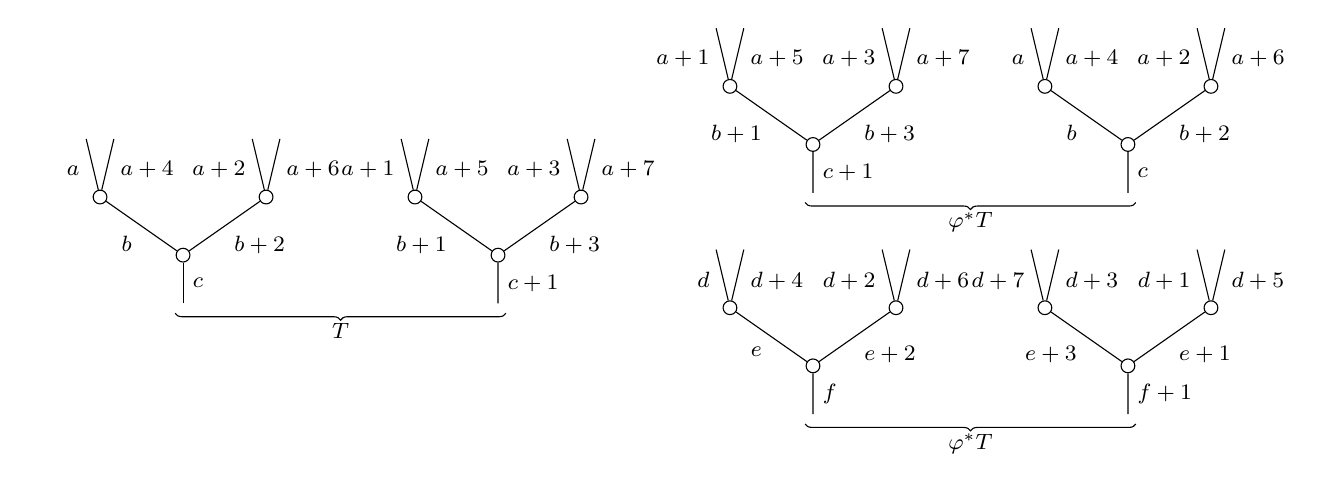
\begin{tikzpicture}[grow=up,auto,level distance=2.1em,every node/.style = {font=\footnotesize},dummy/.style={circle,draw,inner sep=0pt,minimum size=1.75mm}]
		\node at  (0,0) {}
			child{node [dummy] {}
				child[sibling distance = 6em]{node [dummy] {}
					child[sibling distance = 1em]{
					edge from parent node [swap,near end] {$a+6$}}
					child[sibling distance = 1em]{
					edge from parent node [near end] {$a+2$}}
				edge from parent node [swap] {$b+2$}}
				child[sibling distance = 6em]{node [dummy] {}
					child[sibling distance = 1em]{
					edge from parent node [swap,near end] {$a+4$}}
					child[sibling distance = 1em]{
					edge from parent node [near end] {$\phantom{+1}a$}}
				edge from parent node {$b$}}
			edge from parent node [swap] {$c$}};
		\node at  (4,0) {}
			child{node [dummy] {}
				child[sibling distance = 6em]{node [dummy] {}
					child[sibling distance = 1em]{
					edge from parent node [swap,near end] {$a+7$}}
					child[sibling distance = 1em]{
					edge from parent node [near end] {$a+3$}}
				edge from parent node [swap] {$b+3$}}
				child[sibling distance = 6em]{node [dummy] {}
					child[sibling distance = 1em]{
					edge from parent node [swap,near end] {$a+5$}}
					child[sibling distance = 1em]{
					edge from parent node [near end] {$a+1$}}
				edge from parent node {$b+1$}}
			edge from parent node [swap] {$c+1$}};
		\draw[decorate,decoration={brace,amplitude=2.5pt}] (4.1,0) -- (-0.1,0) node[midway]{$T$};
	\begin{scope}[yshift=4em]
		\node at  (12,0) {}
			child{node [dummy] {}
				child[sibling distance = 6em]{node [dummy] {}
					child[sibling distance = 1em]{
					edge from parent node [swap,near end] {$a+6$}}
					child[sibling distance = 1em]{
					edge from parent node [near end] {$a+2$}}
				edge from parent node [swap] {$b+2$}}
				child[sibling distance = 6em]{node [dummy] {}
					child[sibling distance = 1em]{
					edge from parent node [swap,near end] {$a+4$}}
					child[sibling distance = 1em]{
					edge from parent node [near end] {$\phantom{+1}a$}}
				edge from parent node {$b$}}
			edge from parent node [swap] {$c$}};
		\node at  (8,0) {}
			child{node [dummy] {}
				child[sibling distance = 6em]{node [dummy] {}
					child[sibling distance = 1em]{
					edge from parent node [swap,near end] {$a+7$}}
					child[sibling distance = 1em]{
					edge from parent node [near end] {$a+3$}}
				edge from parent node [swap] {$b+3$}}
				child[sibling distance = 6em]{node [dummy] {}
					child[sibling distance = 1em]{
					edge from parent node [swap,near end] {$a+5$}}
					child[sibling distance = 1em]{
					edge from parent node [near end] {$a+1$}}
				edge from parent node {$b+1$}}
			edge from parent node [swap] {$c+1$}};
		\draw[decorate,decoration={brace,amplitude=2.5pt}] (12.1,0) -- (7.9,0) node[midway]{$\varphi^{\**}T$};
	\end{scope}
	\begin{scope}[yshift=-4em]
		\node at  (8,0) {}
			child{node [dummy] {}
				child[sibling distance = 6em]{node [dummy] {}
					child[sibling distance = 1em]{
					edge from parent node [swap,near end] {$d+6$}}
					child[sibling distance = 1em]{
					edge from parent node [near end] {$d+2$}}
				edge from parent node [swap] {$e+2$}}
				child[sibling distance = 6em]{node [dummy] {}
					child[sibling distance = 1em]{
					edge from parent node [swap,near end] {$d+4$}}
					child[sibling distance = 1em]{
					edge from parent node [near end] {$\phantom{+1}d$}}
				edge from parent node {$e$}}
			edge from parent node [swap] {$f$}};
		\node at  (12,0) {}
			child{node [dummy] {}
				child[sibling distance = 6em]{node [dummy] {}
					child[sibling distance = 1em]{
					edge from parent node [swap,near end] {$d+5$}}
					child[sibling distance = 1em]{
					edge from parent node [near end] {$d+1$}}
				edge from parent node [swap] {$e+1$}}
				child[sibling distance = 6em]{node [dummy] {}
					child[sibling distance = 1em]{
					edge from parent node [swap,near end] {$d+3$}}
					child[sibling distance = 1em]{
					edge from parent node [near end] {$d+7$}}
				edge from parent node {$e+3$}}
			edge from parent node [swap] {$f+1$}};
		\draw[decorate,decoration={brace,amplitude=2.5pt}] (12.1,0) -- (7.9,0) node[midway]{$\varphi^{\**}T$};
	\end{scope}
	\end{tikzpicture}
\end{equation}
We note that $(\varphi^{\**}(T))_{v_{G e}} = \psi^{\**}(T_{v_{G b}})$
for $\psi$ the permutation $(13)(24)$ encoded by the composite identifications
$\{1,2,3,4\} \simeq \{e,e+2,e+3,e+1\} \simeq 
\{b+1,b+3,b,b+2\}\simeq \{3,4,1,2\}$.
\end{example}


\begin{lemma}\label{LANPULLCOMA LEM}
	Suppose that $\mathcal{V}$ is complete and that $A \to \Sigma_G$ is a root fibration. If the rightmost triangle in 
	\begin{equation}
	\begin{tikzcd}
		\Omega_{G,0}^{(A)} \ar{r}{V_G^{(A)}} 
		\ar{d} & 
		\Fin \wr A  
		\ar{d}  \ar{r}[swap,name=F]{}&
		\mathcal{V}		
	\\
		\Omega_{G,0} \ar{r}[swap]{V_G} & 
		|[alias=FEG]|\Fin \wr \Sigma_G \ar{ru}
	\arrow[Rightarrow, from=FEG, to=F,shorten <=0.15cm]
	\end{tikzcd}
	\end{equation}
is a right Kan extension diagram then so is the composite diagram.
\end{lemma}


\begin{proof}
	Unpacking definitions using the pointwise formula for right  Kan extensions (\cite[X.3.1]{McL}), 
	it suffices to check that for each $T \in \Omega_{G,0}$ the functor
	\begin{equation}\label{LANPULLCOMA EQ}
	T \downarrow \Omega_{G,0}^{(A)}
	\to 
	V_G(T) \downarrow \Fin \wr A
	\end{equation}
is initial.
In the course of the proof of Lemma \ref{FINWREATPRODLIM LEM}
it was shown that the subcategory
\[
\prod_{v_{Ge} \in V_G(T)} 
T_{v_{Ge}} \downarrow A
\]
is initial in the $V_G(T) \downarrow \Fin \wr A$.

On the other hand, since $\Omega_G^{(A)} \to \Omega_G$ is a root fibration functor, 
$T \downarrow \Omega_{G}^{(A)}$
has an initial subcategory 
$T \downarrow_{\mathsf{r},\simeq} \Omega_{G}^{(A)}$
with objects
$(S \in \Omega_G^{(A)},T \to u(S))$
such that 
$T \to u(S)$
is a quotient map that induces an ordered isomorphism on roots. Note that this can be restated as saying that 
$T \to u(S)$ is an isomorphism preserving the order of the roots.


The result now follows from the natural isomorphism
\begin{equation}\label{TDOWNISOA EQ}
	T \downarrow_{\mathsf{r},\simeq} \Omega_{G}^{(A)} 
\simeq
	\prod_{v_{Ge} \in V_G(T)}
	{T_{v_{Ge}} \downarrow_{\mathsf{r},\simeq} A}.
\end{equation}
To see this, we focus first on the case $A = \Sigma_G$.
In that case, the left hand side of (\ref{TDOWNISOA EQ}) encodes replanarizations of $T$ that preserve the root order.
On the other hand, the right hand side encodes replanarizations of all the $G$-vertices that preserve the order of their roots, or, equivalently, replanarizations of the non-equivariant vertices of $T$.
That these are equivalent is the content of Proposition \ref{PLANARIZATIONCHAR PROP}.

Note that $(T \to S) \in (T \downarrow_{\mathsf{r},\simeq} \Omega_{G})$ is then encoded by a tuple
$\left(T_{v_{Ge}} \to \varphi^{\**}_{v_{Ge}} S_{v_{Ge}}\right)_
{v_{Ge} \in V_G(T)}$
where the pullbacks $\varphi^{\**}_{v_{Ge}}$ are needed to correct the root order.

The case of general $A$ follows likewise, 
using the corresponding pullbacks
$\varphi^{\**}_{v_{Ge}}$.

{\color{red} Note: an addendum is needed to show that (\ref{TDOWNISOA EQ}) suffices, since $T \downarrow_{\mathsf{r},\simeq} \Omega_{G}^{(A)}$ is not sent directly to
 $\prod_{v_{Ge} \in V_G(T)}
	{T_{v_{Ge}} \downarrow_{\mathsf{r},\simeq} A}$}
\end{proof}



Lemma \ref{ROOTFIBPULL LEM} can be interpreted as saying that, if one defines a category
$\mathsf{Wspan}^l_{\mathsf{r}}(\Sigma_G^{op},\mathcal{V})$
of \textit{rooted spans}
\[
\Sigma_G^{op} \leftarrow A^{op} \to \mathcal{V}
\]
where $A \to \Sigma_G$ is a root fibration functor, the monad $N$ built in Proposition \ref{MONSPAN PROP} lifts to a monad 
$N_{\mathsf{r}}$ in
$\mathsf{Wspan}^l_{\mathsf{r}}(\Sigma_G^{op},\mathcal{V})$,
and likewise for the adjunction (\ref{LANIOTAADJ EQ}).

\begin{corollary}
Suppose that finite products in $\mathcal{V}$ commute with colimits in each variable.
The functors
\[
	\mathsf{Lan} \circ N_{\mathsf{r}} \Rightarrow
	\mathsf{Lan} \circ N_{\mathsf{r}} \circ \iota \circ \mathsf{Lan},
\qquad
	\mathsf{Lan} \circ \iota \Rightarrow id
\]
are natural isomorphisms.
\end{corollary}

\begin{proof}
This follows by combining Lemma \ref{LANPULLCOMA LEM} with Lemma \ref{FINWREATPRODLIM LEM}.
\end{proof}


\begin{definition}\label{THEMONAD DEF}
The \textit{genuine equivariant operad monad} is the monad
$\F_G$ on $\mathsf{Fun}(\Sigma_G^{op}, \mathcal{V})$
given by
\[
	\F_G = \mathsf{Lan} \circ N_{\mathsf{r}} \circ \iota
\]
and with multiplication and unit given by the composites
\[
\mathsf{Lan} \circ N_{\mathsf{r}} \circ \iota \circ
\mathsf{Lan} \circ N_{\mathsf{r}} \circ \iota
\overset{\simeq}{\Leftarrow}
\mathsf{Lan} \circ N_{\mathsf{r}} \circ  N_{\mathsf{r}} \circ \iota
\Rightarrow
\mathsf{Lan} \circ N_{\mathsf{r}} \circ \iota
\]
\[
id \overset{\simeq}{\Leftarrow} \mathsf{Lan} \circ \iota
\Rightarrow
\mathsf{Lan} \circ N_{\mathsf{r}} \circ \iota.
\]
We let $\Op_G(\V)$ denote the category $\mathsf{Alg}_{\mathbb F_G}(\V)$ of \textit{genuine equivariant operads}.
\end{definition}


\begin{remark}
	The functor $\mathsf{Lan} \circ N_{\mathsf{r}} \circ \iota$ is isomorphic to 
	$\mathsf{Lan} \circ N \circ \iota$, and this isomorphism is compatible with the multiplication and unit	in Definition \ref{THEMONAD DEF}, and we will henceforth simply write $N$ rather than $N_{\mathsf{r}}$.
	
	From this point of view, the role of root fibrations is to guarantee that $\mathsf{Lan} \circ N \circ \iota$ is indeed a monad, but unnecessary to describe the monad structure itself.
\end{remark}


\begin{remark}\label{REPACKAGERES REM}
Since a map 
\[\F_G X =\mathsf{Lan} \circ N_{\mathsf{r}} \circ \iota X \to X\]
is adjoint to a map
\[N_{\mathsf{r}} \circ \iota X \to \iota X\]
one easily verifies that 
$X$ is a genuine equivariant operad, i.e. 
a $\F_G$-algebra, iff 
$\iota X$ is a $N$-algebra.
Moreover, the bar resolution
\[
	\F_G^{\bullet +1} X 
\]
is isomorphic to
\[
	\mathsf{Lan} \left( N^{\bullet +1} \iota X \right).
\]
\end{remark}


\subsection{Comparison with (regular) equivariant operads}

We start by noting that in the case $G = \**$, genuine operads simply recover the usual notion of symmetric operads, i.e. 
$\mathsf{Sym}_{\**}(\mathcal{V})
\simeq \mathsf{Sym}(\mathcal{V})$
and
$\mathsf{Op}_{\**}(\mathcal{V})
\simeq \mathsf{Op}(\mathcal{V})$, 
and in what follows we will adopt the notations
$\mathsf{Sym}^G(\mathcal{V})$ and
$\mathsf{Op}^G(\mathcal{V})$ 
for the corresponding categories of $G$-objects.
Our goal will be to relate these to the categories
$\mathsf{Sym}_G(\mathcal{V})$ and $\mathsf{Op}_G(\mathcal{V})$
of genuine equivariant sequences and genuine operads.

We will throughout this section fix a total order of $G$ such that the identity $e$ is the first element, though we note that the exact order is unimportant, as any other such choice would lead to unique isomorphisms between the constructions in this section.


We thus have an inclusion functor
\[
\begin{tikzcd}[row sep =0]
	\iota \colon G \times \Sigma \ar[hookrightarrow]{r} &
	\Sigma_G
\\
	C \ar[mapsto]{r} & G \cdot C
\end{tikzcd}
\]
where $G \cdot C$ is planarized so that the roots inherit the order of $G$ and each of the individual copies of $C$ inherits the planarization of $C$.
Moreover, letting $\Sigma_G^{\text{fr}} \hookrightarrow \Sigma_G$ denote the full subcategory of $G$-free corollas, there is an induced retraction 
$\rho \colon \Sigma_{G}^{\text{fr}} \to G \times \Sigma$
defined by 
$\rho(\amalg_{1\leq i \leq |G|} C_i) = G \cdot C_1$
together with isomorphisms 
$C \simeq \rho(C)$
uniquely determined by the condition that they
are the identity on the first tree component $C_1$.


We now consider the associated adjunctions.
\begin{equation}\label{TWOADJOINTS EQ}
\begin{tikzcd}[column sep =5em]
	\mathsf{Sym}_G(\mathcal{V}) \ar{r}[swap]{\iota^{\**}} 
	&
	\mathsf{Sym}^G(\mathcal{V})
	\ar[bend right]{l}[swap,midway]{\iota_{!}}
	\ar[bend left]{l}{\iota_{\**}}
\end{tikzcd}
\end{equation}


Explicitly, we have the formulas
\[
	\iota_!Y(\amalg_i C_i)=
	\begin{cases}
	Y(C_1), & \amalg_i C_i \in \Sigma_G^{\text{fr}} \\
	\emptyset, & \amalg_i C_i \nin \Sigma_G^{\text{fr}}
	\end{cases},
\qquad
	\iota^{\**}X (C) = X(G \cdot C),
\qquad
	\iota_{\**}Y (\amalg_i C_i)=
	\left(\prod_i Y(C_i)\right)^G,
\]
where we note that in the formula for $\iota_{\**}(\minus)$
the action of $G$ interchanges factors according to the action on the indexing set, i.e. the root orbit of $\amalg_i C_i$.
As a side note, we note that the formulas for $\iota_!$ and $\iota_{\**}$ are independent of the chosen order of $G$.

\begin{remark}\label{REFLCOREFL REM}
	$\iota_!$ essentially identifies 
	$\mathsf{Sym}^G(\mathcal{V})$ as the coreflexive subcategory of sequences 
	$X \in \mathsf{Sym}_G(\mathcal{V})$ such that $X(C)=\emptyset$ whenever $C$ is not a free corolla.

By contrast, $\iota_{\**}$ identifies 
$\mathsf{Sym}^G(\mathcal{V})$ with a far more interesting reflexive subcategory of sequences 
$X \in \mathsf{Sym}_G(\mathcal{V})$ 
such that $X(C)$ for each $C$ not a free corolla must satisfy a fixed point condition. Concretely, letting 
$\varphi \colon G \to \mathsf{r}(C)$
denote the unique map preserving the minimal element, one has
\[X(C) \xrightarrow{\simeq} X(\varphi^{\**}C)^{\Gamma}\]
for 
$\Gamma \leq \mathsf{Aut}(\varphi^{\**}C)$
the subgroup preserving the quotient map
$\varphi^{\**}C \to C$
under precomposition (note that $\varphi^{\**}C \in \Sigma_G^{\text{fr}}$).
\end{remark}

There is an obvious natural transformation $\beta \colon \iota_! \Rightarrow \iota_{\**}$ which for 
$\amalg_i C_i \in \Sigma_G^{\text{fr}}$
sends $Y(C_1)$ to the ``$G$-twisted diagonal'' of 
$\prod_i Y(C_i)$.
Moreover, letting $\eta_!,\epsilon_!$ 
(resp. $\eta_{\**},\epsilon_{\**}$)
denote the unit and counit of the $(\iota_!,\iota^{\**})$ adjunction 
(resp. $(\iota^{\**},\iota_{\**})$ adjunction)
it is straightforward to check that the following diagram commutes.
\begin{equation}\label{BETADEFSQUARE EQ}
\begin{tikzcd}
		\iota_{!} \iota^{\**} \iota_{\**}
		\ar[Rightarrow]{r}{\epsilon_!}
		\ar[Rightarrow]{d}{\simeq}[swap]{\epsilon_{\**}}
	&
		\iota_{\**}
		\ar[Rightarrow]{d}{\eta_{!}}[swap]{\simeq}
\\
		\iota_!
		\ar[Rightarrow]{r}[swap]{\eta_{\**}}
		\ar[Rightarrow]{ru}[swap]{\beta}
	&
		\iota_{\**} \iota^{\**} \iota_{!}
\end{tikzcd}
\end{equation}
\begin{remark} An exercise in adjunctions shows that any outer square as in (\ref{BETADEFSQUARE EQ})
 commutes provided at least one of the adjunctions in \ref{TWOADJOINTS EQ} is (co)reflexive, so that (\ref{BETADEFSQUARE EQ}) can be regarded as an alternative definition of $\beta$.
\end{remark}


%By adjunction, one needs compare the composites
%\[
%\iota_{\**} \xrightarrow{\eta_{!}}
%\iota_{\**} \iota^{\**} \iota_{!} 
% \xrightarrow{\iota_{\**} \iota^{\**}\eta_{\**}\iota_{!}}
%\iota_{\**} \iota^{\**} \iota_{\**} \iota^{\**} \iota_{!},
%\qquad
%\iota_{\**} \xrightarrow{\eta_{\**}}
%\iota_{\**} \iota^{\**} \iota_{\**} 
%\xrightarrow{\eta_{!}}
%\iota_{\**} \iota^{\**} \iota_{\**} \iota^{\**} \iota_{!},
%\]
%and the claim comes down to the checking that both maps
%$\iota_{\**} \iota^{\**} \to
%\iota_{\**} \iota^{\**} \iota_{\**} \iota^{\**}$
%coincide, which they do since they have a common inverse.


\begin{proposition}
	One has the following
\begin{itemize}
	\item[(i)]
	the map 
	$\iota^{\**} \mathbb{F}_G
		\xrightarrow{\eta_{\**}}
	\iota^{\**} \mathbb{F}_G \iota_{\**} \iota^{\**}$
	is an isomorphism, 
	and thus (cf. Prop. \ref{MONADADJ PROP})
	$\iota^{\**} \mathbb{F}_G \iota_{\**}$
	is a monad;
	\item[(ii)] the map 
	$\iota^{\**} \mathbb{F}_G \iota_{!}
	\xrightarrow{\beta}	
	\iota^{\**} \mathbb{F}_G \iota_{\**}$ is an isomorphism of monads;
	\item[(iii)] the map 
	$\iota_{!}\iota^{\**} \mathbb{F}_G \iota_{!}
	\xrightarrow{\epsilon_!}
	\mathbb{F}_G \iota_{!}$ is an isomorphism;
	\item[(iv)] there is a natural isomorphism of monads
	$\alpha \colon \mathbb{F} \to \iota^{\**} \mathbb{F}_G \iota_{!}$.
\end{itemize}
\end{proposition}


\begin{proof}
We first show (i), starting with some notation. 
In analogy with $\Sigma_{G}^{\text{fr}}$,
we write $\Omega_{G,0}^{\text{fr}}$ for the subcategory of free trees and note that the leaf-root and vertex functors then restrict to functors
$\mathsf{lr} \colon \Omega_{G,0}^{\text{fr}} \to \Sigma_G^{\text{fr}}$,
$V_G \colon \Omega_{G,0}^{\text{fr}} \to \Fin \wr \Sigma_G^{\text{fr}}$.
Moreover, for each $C \in \Sigma_G^{\text{fr}}$ one has an equality of rooted undercategories between
$C \downarrow_{\mathsf{r}} \Omega_{G,0}$
and
$C \downarrow_{\mathsf{r}} \Omega_{G,0}^{\text{fr}}$,
and thus 
$\iota^{\**} \mathbb{F}_G X$ is computed by the Kan extension of the following diagram.
\begin{equation}\label{IFGI EQ}
\begin{tikzcd}
	\Omega_{G,0}^{\text{fr}} \ar{d} \ar{r} &
	\Fin \wr \Sigma_G^{\text{fr}} \ar{r}{\Fin \wr X} &
	\Fin \wr \mathcal{V}^{op} \ar{r} &
	\mathcal{V}^{op}
\\
	\Sigma_G^{\text{fr}}
\end{tikzcd}
\end{equation}
(i) now follows by noting that 
$X \to \iota_{\**} \iota^{\**} X$
is an isomorphism when restricted to $\Sigma_G^{\text{fr}}$.

For (ii), to show that 
	$\iota^{\**} \mathbb{F}_G \iota_{!}
	\to	
	\iota^{\**} \mathbb{F}_G \iota_{\**}$ is an isomorphism one just repeats the argument in the previous paragraph by noting  that $\iota_! \to \iota_{\**}$ is an isomorphism when restricted to $\Sigma_G^{\text{fr}}$.
	To check that this is a map of monads, we recall first that the monad structure on $\iota^{\**} \mathbb{F}_G \iota_{\**}$
is given as described in Proposition \ref{MONADADJ PROP}.
Unpacking definitions, compatibility with multiplication reduces to showing that the composite 
$\iota_! \iota^{\**} \xrightarrow{\epsilon_!} 
id \xrightarrow{\eta_{\**}} \iota_{\**} \iota^{\**}$
coincides with $\beta \iota^{\**}$
while compatibility with units 
reduces to showing that the composite
$
	id \xrightarrow{\eta_!} 
	\iota^{\**} \iota_! \xrightarrow{\iota^{\**} \beta}
	\iota^{\**} \iota_{\**} \xrightarrow{\epsilon_{\**}}
	id
$
is the identity. Both of these are a consequence of 
(\ref{BETADEFSQUARE EQ}), following from the diagrams below 
(where the top composites are identities).
\begin{equation}
\begin{tikzcd}[column sep =3em]
		\iota_! \iota^{\**}
		\ar[Rightarrow]{r}{\iota_! \iota^{\**} \eta_{\**}}
		\ar[Rightarrow]{d}[swap]{\epsilon_!}
	&
		\iota_{!} \iota^{\**} \iota_{\**} \iota^{\**}
		\ar[Rightarrow]{d}[swap]{ \epsilon_! \iota_{\**}\iota^{\**}}
		\ar[Rightarrow]{r}[swap]{\simeq}{\iota_{!}\epsilon_{\**}\iota^{\**}}
	&
		\iota_! \iota^{\**}
		\ar[Rightarrow]{ld}{\beta \iota^{\**}}
	&	
		\iota^{\**} \iota_{\**}
		\ar[Rightarrow]{r}{\eta_! \iota^{\**} \iota_{\**}}[swap]{\simeq}
		\ar[Rightarrow]{d}[swap]{\epsilon_{\**}}{\simeq}
	&
		\iota^{\**} \iota_{!} \iota^{\**} \iota_{\**}
		\ar[Rightarrow]{r}{\iota^{\**} \epsilon_! \iota_{\**}}
		\ar[Rightarrow]{d}{\simeq}[swap]{\iota^{\**}\iota_{!}\epsilon_{\**}}
	&
		\iota^{\**}\iota_{\**}
\\
		id
		\ar[Rightarrow]{r}[swap]{\eta_{\**}}
	&
		\iota_{\**} \iota^{\**}
	&
	&	
		id
		\ar[Rightarrow]{r}[swap]{\eta_!}{\simeq}
	&
		\iota^{\**} \iota_!
		\ar[Rightarrow]{ru}[swap]{\iota^{\**} \beta}
\end{tikzcd}
\end{equation}

(iii) amounts to showing that if $X(C) =\emptyset$ whenever 
$C \nin \Sigma_G^{\text{fr}}$
then it is also 
$\mathbb{F}_G X(C) =\emptyset$.
But since for such 
$C \nin \Sigma_G^{\text{fr}}$
the undercategory
$C \downarrow \Omega_{G,0}$
consists of trees with at least one non-free vertex, the composite
\[
\begin{tikzcd}
	C \downarrow \Omega_{G,0} \ar{r}{V} &
	\Fin \wr \Sigma_G \ar{r}{\Fin \wr X} &
	\Fin \wr \mathcal{V}^{op} \ar{r}{\Pi}&
	\mathcal{V}^{op}
\end{tikzcd}
\]
is constant equal to $\emptyset$, and (iii) follows.


Finally, we show (iv). We will slightly abuse notation by writing 
$G \times \Sigma \hookrightarrow \Sigma_G$ for the image of $\iota$
and similarly
$G \times \Omega_0 \hookrightarrow \Omega_{G,0}$ for the image of the obvious analogous functor
$\iota \colon G \times \Omega_0 \to \Omega_{G,0}$.
The map 
$\alpha \colon \mathbb{F} \to \iota^{\**} \mathbb{F}_G \iota_{!}$
is the adjoint to the map 
$\tilde \alpha: \mathbb{F} \iota^{\**} \to \iota^{\**} \mathbb{F}_G$ encoded on spans by the following diagram.
\begin{equation}\label{MONADEQUIV DEF}
\begin{tikzcd}[row sep=5pt, column sep =8pt]
	G \times \Omega_0	\ar{dd} \ar{rd} \ar{rr} &&
	\Fin \wr (G \times \Sigma_0) \ar{rd}  \ar{rr}{\iota^{\**} X}&&
	\Fin \wr \mathcal{V}^{op} \ar{r} \ar[equal]{rd}&
	\mathcal{V}^{op} \ar[equal]{rd}
\\
	& \Omega_{G,0} \ar{dd} \ar{rr} &&
	\Fin \wr \Sigma_G  \ar{rr}[swap]{X} &&
	\Fin \wr \mathcal{V}^{op} \ar{r} &
	\mathcal{V}^{op}
\\
	G \times \Sigma \ar{rd} 
\\
	& \Sigma_G
\end{tikzcd}
\end{equation}
That 
$\alpha$
is a natural isomorphism
follows by the previous identifications 
$C \downarrow_{\mathsf{r}} \Omega_{G,0} \simeq
C \downarrow_{\mathsf{r}} \Omega_{G,0}^{\text{fr}}$
for $C \in G \times \Sigma$
together with the fact that the retraction 
$\rho \colon \Omega_{G,0}^{\text{fr}} \to G \times \Omega_0$
(built just as the retraction
$\rho \colon \Sigma_G^{\text{fr}} \to G \times \Sigma$)
retracts 
$C \downarrow_{\mathsf{r}} \Omega_{G,0}^{\text{fr}}$
to the undercategory
$C \downarrow_{\mathsf{r}} G \times \Omega_0$, which is thus initial (as well as final), and the claim that $\alpha$ is an isomorphism follows.

Intuitively, the final claim that 
$\alpha$ is a map of monads 
follows from the fact that the composite 
$
\mathbb{F} \mathbb{F}
	\to 
\iota^{\**} \mathbb{F}_G \iota_{!} \iota^{\**} \mathbb{F}_G \iota_{!}
	\to
\iota^{\**} \mathbb{F}_G \mathbb{F}_G \iota_{!}
$
is encoded by the analogous natural transformation of diagrams for strings $G \times \Omega_1 \hookrightarrow \Omega_{G,1}^{\text{fr}}$.
However, since the presence of left Kan extensions in the 
definitions of $\mathbb{F}$, $\mathbb{F}_G$
can make a rigorous direct proof of this last claim fairly cumbersome, we sketch here a workaround argument.
We first consider the adjunction
$
	\iota_{!} \colon
	\mathsf{WSpan}^l((G\times \Sigma)^{op},\mathcal{V})
		\rightleftarrows
	\mathsf{WSpan}^l(\Sigma_G^{op},\mathcal{V})
	\colon \iota^{\**}
$
where $\iota_!$ is composition with $\iota$ and $\iota^{\**}$ is the pullback of spans. 
Writing $N$, $N_G$ for the monads 
on the span categories, mimicking (\ref{MONADEQUIV DEF}) yields
a map 
$\tilde{\alpha} \colon N \to \iota^{\**} N_G \iota_{!}$
encoded by the diagram (where the front and back squares are pullbacks).
\[
\begin{tikzcd}[row sep=3pt, column sep =8pt]
	(G \times \Omega)^{(\iota^{\**} A)}	\ar{dd} \ar{rd} \ar{rr} &&
	\Fin \wr \iota^{\**} A \ar{rd} \ar[dashed]{dd} \ar{rr}&&
	\Fin \wr \mathcal{V}^{op} \ar{r} \ar[equal]{rd} &
	\mathcal{V}^{op} \ar[equal]{rd}
\\
	& \Omega_{G,0}^{(A)} \ar{dd} \ar{rr} &&
	\Fin \wr A \ar{dd} \ar{rr} &&
	\Fin \wr \mathcal{V}^{op} \ar{r} &
	\mathcal{V}^{op}
\\
	G \times \Omega_0	\ar{dd} \ar{rd} \ar[dashed]{rr}&&
	\Fin \wr (G \times \Sigma) \ar[dashed]{rd}
\\
	& \Omega_{G,0} \ar{dd} \ar{rr} &&
	\Fin \wr \Sigma_G
\\
	G \times \Sigma \ar{rd}
\\
	& \Sigma_{G}
\end{tikzcd}
\]
The claim that $\tilde{\alpha}$ is a map of monads is then straightforward. Writing
\[
	\mathsf{Lan} \colon
	\mathsf{WSpan}^l((G\times \Sigma)^{op},\mathcal{V})
		\rightleftarrows
	\mathsf{Fun}((G\times \Sigma)^{op},\mathcal{V})
	\colon j
\quad
	\mathsf{Lan}_G \colon
	\mathsf{WSpan}^l(\Omega_G^{op},\mathcal{V})
		\rightleftarrows
	\mathsf{Fun}(\Omega_G^{op},\mathcal{V})
	\colon j_G
\]
for the span functor adjunctions,  
$\alpha \colon \mathbb{F} \to \iota^{\**} \mathbb{F}_G \iota_{!}$ can then be written as the composite
\[
	\mathsf{Lan} N j \to 
	\mathsf{Lan} \iota^{\**} N_G \iota_! j  \to
	\iota^{\**} \mathsf{Lan}_G  N_G  j_G \iota_!
\]
where the first map is the isomorphism of monads induced by $\tilde{\alpha}$ and the second map can be shown directly to be a monad map by unpacking the monad structures in 
Propositions \ref{MONADADJ1 PROP} and \ref{MONADADJ PROP}.
%\[
%\begin{tikzcd}
%	(G \times \Omega_1)^{(\iota^{\**} A)}	\ar{ddd} \ar{rd} \ar{rrr} &&&
%	\Fin \wr (G \times \Omega_0)^{(\iota^{\**} A)} \ar{rd} \ar[dashed]{ddd} 
%\\
%	& \bullet \ar{rrr} \ar{ldd} \ar{rd}&&&
%	\Fin \wr \iota^{\**} \left( \Omega_G^{(A)} \right)
%	\ar[dashed]{ldd}\ar{rd}
%\\
%	& & \Omega_1^{(A)} \ar{rrr} \ar{ddl}&&&
%	\Fin \wr \Omega_G^{(A)}\ar{ddl}
%\\
%	G \times \Omega_0	\ar{dd} \ar{rd} \ar[dashed]{rrr}&&&
%	\Fin \wr (G \times \Sigma) \ar[dashed]{rd}
%\\
%	& \Omega_{G,0} \ar{dd} \ar{rrr} &&&
%	\Fin \wr \Sigma_G
%\\
%	G \times \Sigma \ar{rd}
%\\
%	& \Sigma_{G}
%\end{tikzcd}
%\]
%to check second map is monad map, need to show
%\[
%\begin{tikzcd}
%	\iota_{!} \iota^{\**} \ar{d}{\simeq}[swap]{\eta_{\mathsf{Lan}}} \ar{rd}{\epsilon_!}
%\\	
%	\iota_! j \mathsf{Lan} \iota^{\**} \ar{d}&
%	id \ar{d}{\eta_{\mathsf{Lan}_G}}
%\\
%	j_G \iota_! \iota^{\**} \mathsf{Lan}_G \ar{r}{\epsilon_!} & %j_G \mathsf{Lan}_G
%\end{tikzcd}
%\]
%which after two adjunctions becomes
%\[
%\begin{tikzcd}
%	id \ar{d}{\eta_{\mathsf{Lan}}} \ar{r}{\eta_{!}} &
%	\iota^{\**} \iota_! \ar{ddd}{\eta_{\mathsf{Lan}_G}}
%\\
%	j \mathsf{Lan} \ar{d}{\eta_! \eta_!}
%\\
%	j \iota^{\**} \iota_{!} \iota^{\**} \iota_{!} \mathsf{Lan}
%	\ar[equal]{d}
%\\
%	\iota^{\**} j_G \iota_{!} \iota^{\**} \mathsf{Lan}_G \iota_{!} \ar{r}{\epsilon_!}& \iota^{\**} j_G \mathsf{Lan}_G \iota_!
%\end{tikzcd}
%\]
\end{proof}


Combining the previous result with
Propositions \ref{MONADADJ1 PROP} and \ref{MONADADJ PROP} now gives the following.

\begin{corollary}
	The adjunctions (\ref{TWOADJOINTS EQ}) extends to  adjunctions
\begin{equation}\label{TWOADJOINTSOP EQ}
\begin{tikzcd}[column sep =5em]
	\mathsf{Op}_G(\mathcal{V}) \ar{r}[swap]{\iota^{\**}} 
	&
	\mathsf{Op}^G(\mathcal{V})
	\ar[bend right]{l}[swap,midway]{\iota_{!}}
	\ar[bend left]{l}{\iota_{\**}}.
\end{tikzcd}
\end{equation}
In particular, $\iota_{\**}$
identifies $\mathsf{Op}^G$ as a reflexive subcategory of 
$\mathsf{Op}_G$.
\end{corollary}

\begin{remark}
	Remark \ref{REFLCOREFL REM} extends to operads mutatis mutandis.
	
Moreover, the isomorphism
	$\iota_{!}\iota^{\**} \mathbb{F}_G \iota_{!}
	\xrightarrow{\epsilon_!}
	\mathbb{F}_G \iota_{!}$
then shows that $\mathbb{F}_G$ essentially preserves the image of $\iota_!$, and can thus be identified with $\mathbb{F}$ over it.

However, the analogous statement fails for $\iota_{\**}$, i.e., one does not always have that
\begin{equation}\label{KEYNONISO EQ}
	\mathbb{F}_G \iota_{\**}
	\xrightarrow{\eta_{\**}}
	\iota_{\**}\iota^{\**} \mathbb{F}_G \iota_{\**}
\end{equation}
is an isomorphism. 
In fact, showing that (\ref{KEYNONISO EQ})
\textit{does} become an isomorphism when restricted to suitably cofibrant objects is one of the key technical ingredients for our proof of the Quillen equivalence between 
$\mathsf{Op}_G(\mathcal{V})$ and
$\mathsf{Op}^G(\mathcal{V})$, 
and will be the subject of \S \ref{COFIB SEC}.

For now, we end this section with a minimal counterexample to  the more general claim.

Let $G=\mathbb{Z}_{/2}$ and 
$Y=\** \in \mathsf{Sym}^G(\mathcal{V})$ be the simpleton.

	When evaluating $\mathbb{F}_G Y$ at the $G$-fixed stump corolla $G/G \cdot C_0$, the two $G$-trees $T_1$ and $T_2$ below encode two distinct points (since $T_1$, $T_2$ are not isomorphic as objects under $G/G\cdot T_0$).
\[
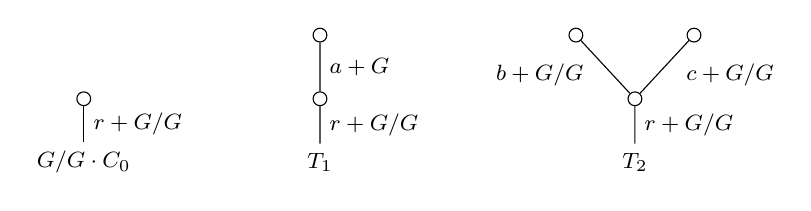
\begin{tikzpicture}[grow=up,auto,level distance=2.3em,every node/.style = {font=\footnotesize},dummy/.style={circle,draw,inner sep=0pt,minimum size=1.75mm}]
	\node at (0,0) {$G/G \cdot C_0$}
		child{
			node [dummy] {}
		edge from parent node [swap] {$r+G/G$}};
	\node at (3,0) {$T_1$}
		child{node [dummy] {}
			child{node [dummy] {}
			edge from parent node [swap] {$a+G$}}
		edge from parent node [swap] {$r+G/G$}};
	\node at (7,0) {$T_2$}
		child{node [dummy] {}
			child{node [dummy] {}
			edge from parent node [swap,near end] {$c+G/G$}}
			child{node [dummy] {}
			edge from parent node [near end] {$b+G/G$}}
		edge from parent node [swap] {$r+G/G$}};
\end{tikzpicture}
\]
However, when pulling these points back to the $G$-free stump corolla $G \cdot C_0$ one obtains the same point, namely that encoded by the $G$-tree $T$ below.
\[
\begin{tikzpicture}[grow=up,auto,level distance=2.3em,every node/.style = {font=\footnotesize},dummy/.style={circle,draw,inner sep=0pt,minimum size=1.75mm}]
	\node at (0,0) {$G \cdot C_0$}
		child{
			node [dummy] {}
		edge from parent node [swap] {$r+G$}};
	\node at (5,0) {$T$}
		child{node [dummy] {}
			child{node [dummy] {}
			edge from parent node [swap,near end] {$c+G$}}
			child{node [dummy] {}
			edge from parent node [near end] {$b+G$}}
		edge from parent node [swap] {$r+G$}};
\end{tikzpicture}
\]
Moreover, it is not hard to modify the example above to produce similar examples when evaluating $\mathbb{F}_GY$ at non-empty corollas. 

However, such counter-examples all require the use of trees with stumps. Indeed, it can be shown that (\ref{KEYNONISO EQ})
is an isomorphism whenever evaluated at a $Y$ such that $Y(C_0)=\emptyset$.
\end{remark}



\section{Free extensions}
\label{FREE_EXTENSIONS_SECTION}

Our overall goal in this section will be to produce a description of free $\mathbb F_G$-extensions,  %genuine operad pushouts,
i.e. pushouts of the form
\[
\begin{tikzcd}
	\mathbb{F}_G A \ar{r} \ar{d} & X \ar{d}
\\
	\mathbb{F}_G B \ar{r} & Y
\end{tikzcd}
\]
in the category $\mathsf{Op}_G$ of genuine equivariant operads.



\subsection{Extensions over general monads}\label{EXTGENMON SEC}

Any monad $T$ on $\C$ one obtains induced monads $T^{\times l}$ on $\C^{\times l}$, and we will make use of several standard relations between these.
In particular, any map $\alpha \colon \underline{l} \to \underline{m}$ induces a forgetful functor
such that for the forgetul functor 
$\alpha^{\**} \colon \C^{\times l} \to \C^{\times n}$
one has $T^{\times l} \alpha^{\**} \simeq  \alpha^{\**} T^{\times m}$.


Indeed, we will need to make use of a slightly more general setup. Letting $I$ denote the identity monad on $\C$, and $K \subset \underline{m}$ be a subset, there is a monad $T^{\times K} \times I^{\times(\underline{m}-K)}$ on $\mathcal{C}^{\times m}$, which we abusively denote simply as $T^{\times K}$. Identities then determine maps of monads 
$T^{\times J} \to T^{\times K}$ whenever $J \subset K$
and, moreover, there are identifications
$T^{\times \alpha^{-1}(K)} \alpha^{\**} \simeq \alpha^{\**} T^{\times K}$.
One then has the following.


\begin{proposition}\label{MONADICFUN PROP}
	The functor
\begin{equation}\label{MONADFUNCTORALPHA EQ}
	T^{\times \alpha^{-1} (K)} \Rightarrow \alpha^{\**} T^{\times K} \alpha_{!}
\end{equation}
adjoint to the identification 
$T^{\times \alpha^{-1} (K)} \alpha^{\**} \simeq \alpha^{\**} T^{\times K}$
is a map of monads on $\C^{\times n}$.
\end{proposition}


\begin{proof}
We first note that there are identifications of functors
$(FG)^{\times K} \simeq F^{\times K} G^{\times K}$ which are compatible with the identifications
$F^{\times \alpha^{-1} (K)} \alpha^{\**} \simeq \alpha^{\**} F^{\times K}$
in the sense that the identification
$(F G)^{\times \alpha^{-1} (K)} \circ \alpha^{\**} \simeq 
\alpha^{\**} (FG)^{\times K}$
matches the composite identification
$F^{\times \alpha^{-1} (K)} G^{\times \alpha^{-1} (K)} \alpha^{\**} \simeq
F^{\times \alpha^{-1} (K)}\alpha^{\**}G^{\times K} \simeq
\alpha^{\**} F^{\times K} G^{\times K}$.

Letting $\eta, \epsilon$ denote the unit and counit for the 
$(\alpha_{!},\alpha^{\**})$ adjunction, 
(\ref{MONADFUNCTORALPHA EQ})
is then the composite
\[
	T^{\times \alpha^{-1} (K)} \xrightarrow{\eta} 
	T^{\times \alpha^{-1} (K)} \alpha^{\**} \alpha_{!} \simeq
	\alpha^{\**} T^{\times K}\alpha_{!}.
\]
That this is a monad map is the condition that the following multiplication and unit diagrams commute.
\[
\begin{tikzcd}
	T^{\times \alpha^{-1} (K)} \circ T^{\times \alpha^{-1} (K)} \ar{d} \ar{r} &
	\alpha^{\**} T^{\times K} \alpha_{!} \circ 
	\alpha^{\**} T^{\times K} \alpha_{!} \ar{d} &
	I^{\times n} \ar{d} \ar{rd}& 	
\\
	T^{\times \alpha^{-1} (K)} \ar{r} &
	\alpha^{\**} T^{\times K} \alpha_{!} &
	T^{\times \alpha^{-1} (K)} \ar{r} &
	\alpha^{\**} T^{\times K} \alpha_{!}
\end{tikzcd}
\]
We argue only the case of the leftmost multiplication diagram, with commutativity of the unit diagram following by a similar but simpler argument. Since precomposition
$(\minus) \circ \alpha^{\**}$
is left adjoint to precomposition
$(\minus) \circ \alpha_{!}$
this follows from the following commutative diagram.
\[
\begin{tikzcd}[column sep=1.5em]
	T^{\times \alpha^{-1} (K)}  T^{\times \alpha^{-1} (K)}  \alpha^{*} \ar{r}{\simeq} \ar{dd}&
	T^{\times \alpha^{-1} (K)}  \alpha^{*}  T^{\times K} \ar{r}{\eta}
	\ar[equal]{rd} &
	T^{\times \alpha^{-1} (K)} \alpha^{\**} \alpha_{!} \alpha^{*} T^{\times K} \ar{d}{\epsilon} \ar{r}{\simeq}&
	\alpha^{\**} T^{\times K} \alpha_{!} \alpha^{\**}  T^{\times K} \ar{d}{\epsilon}
\\
	& &
	T^{\times \alpha^{-1} (K)}  \alpha^{*}  T^{\times K} \ar{r}{\simeq} &
	\alpha^{*}  T^{\times K}  T^{\times K} \ar{d}
\\
	T^{\times \alpha^{-1} (K)}  \alpha^{*} \ar{rrr}{\simeq} &&&
	\alpha^{*} T^{\times K}
\end{tikzcd}
\]
\end{proof}


\begin{remark}\label{TALPHAKMOD REM}
	Since $T^{\times K} \alpha_{!}$ is a right 
	$\alpha^{\**} T^{\times K}\alpha_{!}$-module,
	Proposition \ref{MONADICFUN PROP} implies that it is also a 
	right $T^{\times \alpha^{-1}(K)}$-module or, moreover, a 
	right $T^{\times J}$-module whenever $\alpha(J) \subset K$.
\end{remark}


\begin{remark}\label{PRECOMPPOSTCOMP REM}
Combining the precomposition and postcomposition adjunctions,
the identification 
$T^{\times \alpha^{-1} (K)} \alpha^{\**} \simeq \alpha^{\**} T^{\times K}$
is then adjoint to a functor
$	\alpha_{!} T^{\times \alpha^{-1} (K)} 
	\to
	T^{\times K} \alpha_{!}$
which is readily checked to be a map of right $T^{\times \alpha^{-1} (K)}$-modules.

More generally, for $\alpha(J) \subset K$, the composite 
$T^{\times J}\alpha^{\**} \to T^{\times \alpha^{-1} (K)} \alpha^{\**} \simeq \alpha^{\**} T^{\times K}$ is thus adjoint to a map of right $T^{\times J}$-modules
\begin{equation}\label{RIGHTMODULETMAP EQ}
	\alpha_{!} T^{\times J} \to T^{\times K} \alpha_{!}.
\end{equation}
We now unpack the content of (\ref{RIGHTMODULETMAP EQ}) when 
$\alpha \colon \underline{l} \to \**$ is the unique map to the simpleton $\** = \underline{1}$. In this case we can instead write $\alpha_{!} = \coprod$, $\alpha^{\**}=\Delta$,
and we thus have commutative diagrams
\begin{equation}\label{RIGHTMODULETMAPAUX EQ}
\begin{tikzcd}
	\coprod_{J} TT A_j \amalg \coprod_{\underline{l}-J} A_j
	\ar{r} \ar{d} &
	T\left( \coprod_{J} T A_j \amalg \coprod_{\underline{l}-J} A_j \right) \ar{d}
\\
	\coprod_{J} T A_j \amalg \coprod_{\underline{l}-J} A_j
	\ar{r} &
		T\left( \coprod_{J} A_j \amalg \coprod_{\underline{l}-J} A_j \right)
\end{tikzcd}
\end{equation}
for each collection $\left( A_j \right)_{j\in\underline{l}}$ in $\mathcal{C}$,
where the vertical maps
come from the right $T^{\times J}$-module structure.
Writing $\amalg^a$ for the coproduct of $T$-algebras and recalling the canonical identifications 
$\coprod^a_K (T A_k) \simeq T\left( \coprod_K A_k \right)$, 
(\ref{RIGHTMODULETMAPAUX EQ}) in fact shows that the 
right $T^{\times J}$-module structure on $T \circ \coprod$
in fact codifies the multiplication maps
\[
\coprod^a_J TT A_j \amalg^a \coprod^a_{\underline{l}-J} T A_j
	\to
\coprod^a_J T A_j \amalg^a \coprod^a_{\underline{l}-J} T A_j.
\] 
\end{remark}


\subsection{Labeled planar strings}\label{LABELSTRI SEC}

We now translate the results in the previous section to the context of the monad $N$ on $\mathsf{WSpan}^l(\Sigma^{op},\mathcal{V})$. In analogy to the planar string models $\Omega_{G,n}^{(A)}$ for iterations $N^{\circ n+1}$ of the monad $N$,
we will find it convenient to build similar string models
$\Omega_{G,n}^{(\underline{A}_J)}$ for 
$N \circ \coprod \circ (N^{\times J})^{\circ n}$.


\begin{definition}
A \textit{$l$-node labeled $G$-tree} (or just \textit{$l$-labeled $G$-tree}) $G$-tree is a pair $(T,V_G(T) \to \{1,\cdots,l\})$ with $T \in \Omega_G$, which we think of as a $G$-tree together with $G$-vertices labels in $1,\cdots,l$.

Further, a tall map $\varphi \colon T \to S$ between $l$-labeled trees is called a \textit{label map} if for each $G$-vertex $v_{G e}$ of $T$ with label $j$, the vertices of the subtree $S_{v_{G e}}$ are all labeled by $j$.

Lastly, given a subset $J\subset \underline{l}$, a planar label map $\varphi \colon T \to S$ is said to be $J$-inert if for every $G$-vertex $v_{G e}$ of $T$ with label $j \in J$ it is $S_{v_{Ge}} = T_{v_{Ge}}$.
\end{definition}


\begin{example}\label{LABELEDTREES EX}
Consider the $2$-labeled trees below (for $G=\**$ the trivial group), with black nodes ($\bullet$) denoting labels by the number $1$ and white nodes ($\circ$) labels by the number $2$.
The planar map $\varphi$ (sending $a_i\mapsto a$, 
$b \mapsto b$, $c \mapsto c$, $d \mapsto d$, $e \mapsto e$) is a label map which is $\{1\}$-inert.
\begin{equation}\label{SUBSDATUMTREESLAB EQ}
	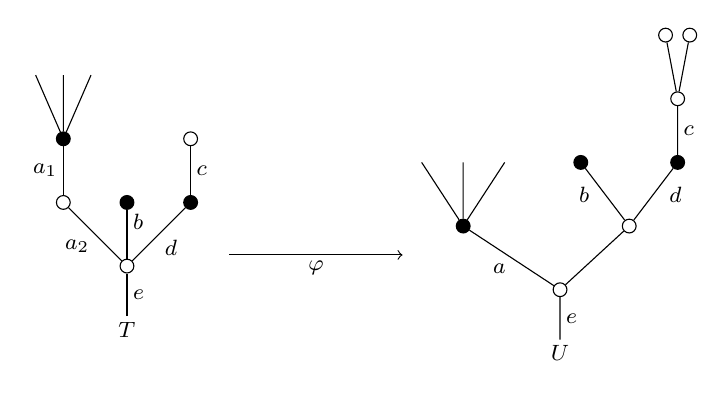
\begin{tikzpicture}[grow=up,auto,level distance=2.1em,
	every node/.style = {font=\footnotesize,inner sep=2pt},
	dummy/.style={circle,draw,inner sep=0pt,minimum size=1.75mm}]
	\begin{scope}[level distance=2.3em]
	\tikzstyle{level 2}=[sibling distance=3.5em]%
	\tikzstyle{level 3}=[sibling distance=2.25em]%
	\tikzstyle{level 4}=[sibling distance=1.25em]%
	\tikzstyle{level 5}=[sibling distance=0.875em]%
		\node at (5.5,0) {$U$}
			child{node [dummy] {}
				child[sibling distance =5em]{node [dummy] {}
					child[sibling distance =3.5em]{node [dummy,fill=black] {}
						child{node [dummy] {}
							child{node [dummy] {}}
							child{node [dummy] {}}
						edge from parent node [swap] {$c$}}
					edge from parent node [swap, near end] {$d$}}
					child[sibling distance =3.5em]{node [dummy,fill=black] {}
					edge from parent node [near end] {$b$}}
				}
				child[sibling distance =7em]{node [dummy,fill=black] {}
					child[sibling distance =1.5em]
					child[sibling distance =1.5em]
					child[sibling distance =1.5em]
				edge from parent node {$a$}}
			edge from parent node [swap] {$e$}};
	\end{scope}
	\begin{scope}[level distance=2.3em]
	\tikzstyle{level 2}=[sibling distance=2.3em]%
	\tikzstyle{level 4}=[sibling distance=1em]%
		\node at (0,0.3) {$T$}
			child{node [dummy] {}
				child{node [dummy,fill=black] {}
					child{node [dummy] {}
					edge from parent node [swap] {$c$}}	
				edge from parent node [swap] {$d$}}
				child{node [dummy,fill=black] {}
				edge from parent node [near end,swap] {$b$}}
				child{node [dummy] {}
					child{node [dummy,fill=black] {}
						child
						child
						child
					edge from parent node {$a_1$}}
				edge from parent node {$a_2$}}
			edge from parent node [swap] {$e$}};
	\end{scope}
	\draw [->] (1.3,1.25) -- node[swap] {$\varphi$} (3.5,1.25);
	\end{tikzpicture}
\end{equation}
\end{example}



\begin{definition}
Let $0 \leq s \leq n$ and $J \subset \underline{l}$ be a subset.

We define $\Omega_{G,n,s}^{J}$ to have as objects $n$-planar strings
\begin{equation}\label{NSTRINGLAB EQ}
	T_0 \xrightarrow{f_1}
	T_1 \xrightarrow{f_2}
	\cdots \xrightarrow{f_s}
	T_s \xrightarrow{f_{s+1}}
	T_{s+1} \xrightarrow{f_{s+2}}
	\cdots \xrightarrow{f_n}
	T_{n}
\end{equation}
together with
$l$-labelings of $T_s, T_{s+1},\cdots, T_{n}$ such that the $f_r,r>s$ are $(\underline{l}-J)$-inert label maps.

Arrows in $\Omega_{G,n,s}^{J}$ are quotients of strings
$(q_r \colon T_r \to T'_r)$ such that 
$q_r,r\leq s$ are label maps.
\end{definition}

Informally, $\Omega_{G,n,s}^{\underline{l}}$ consists of $n$-strings such that trees and maps after $T_s$ are $l$-labeled.

\begin{remark} 
Our main case of interest will that of $s=0$, in which case we abbreviate 
$\Omega_{G,n}^{J} = \Omega_{G,n,0}^{J}$.
Indeed, such strings will suffice to build models for $N \circ \coprod \circ (N^{\times J})^{\circ n}$.

However, to unpack the right $N^{\times J}$-module structure as in Remark \ref{TALPHAKMOD REM} one further needs to encode composites $NN \circ \coprod \circ (N^{\times J})^{\circ n-1}$, 
a role played by strings $\Omega_{G,n,1}^{J}$.
\end{remark}

\begin{notation}
	We will further write 
\begin{equation}\label{OMEGANMINUSONE EQ}
	\Omega_{G,n,-1}^{J} = \coprod_J \Omega_{G,n} \amalg \coprod_{\underline{l}-J} \Sigma_G,
	\qquad
	\Omega_{G,n,n+1}^{J} = \Omega_{G,n}
\end{equation}
To justify this convention, we note that a string as in (\ref{NSTRINGLAB EQ}) can be extended by prepending to it the map $\mathsf{lr}(T_0) = T_{-1} \xrightarrow{f_0} T_0$. If one then attempts to define $\Omega_{G,n,-1}^{J}$ by insisting that  $T_{-1}$ also be labeled, it follows that all node labels in each string must coincide, resulting in the coproduct decomposition in (\ref{OMEGANMINUSONE EQ}).
\end{notation}


There are a number of obvious functors relating the $\Omega_{G,n,s}^{J}$ categories, which we now make explicit.
Given $s\leq s'$ or $J \subset J'$ there are forgetful functors
\begin{equation}\label{NKNFGT EQ}
	\Omega_{G,n,s}^{J} \to \Omega_{G,n,s'}^{J}
\qquad
	\Omega_{G,n,s}^{J} \to \Omega_{G,n,s}^{J'}
\end{equation}
The simplicial operators in Notation \ref{SIMPOPERATORS NOT}
generalize to operators (where $0 \leq i \leq n$, $-1\leq j \leq n$)
\[
\begin{tikzcd}[row sep =0,column sep =1em]
	d_i \colon 
	\Omega_{G,n,s}^{J} \ar{r} &
	\Omega_{G,n-1,s-1}^{J} &
	i < s & & & &
	s_j \colon 
	\Omega_{G,n,s}^{J} \ar{r} &
	\Omega_{G,n+1,s+1}^{J} &
	j < s
\\
	d_i \colon 
	\Omega_{G,n,s}^{J} \ar{r} &
	\Omega_{G,n-1,s}^{J} &
	s \leq i & & & &
	s_j \colon 
	\Omega_{G,n,s}^{J} \ar{r} &
	\Omega_{G,n+1,s}^{J} &
	s \leq j
\end{tikzcd}
\]
which are compatible with the forgetful functors in the obvious way.


\begin{remark}
	For $J \subset J'$ the forgetful functor in (\ref{NKNFGT EQ}) is a fully faithful inclusion. 
	However, and somewhat subtly, this is not the case the for the $ s \leq s'$ forgetful functors. Indeed, regarding
	$T \to U$ in Examples \ref{LABELEDTREES EX} as an object in 
	$\Omega_{\**,n,0}^{\underline{2}}$, changing the label of the $a_1 \leq a_2$ vertex of $T$ from a $\circ$-label to a $\bullet$-label yields an alternate object $\bar{T} \to U$
	of $\Omega_{\**,n,0}^{\underline{2}}$ forgetting to the same object of $\Omega_{\**,n,1}^{\underline{2}}$, yet $T \to U$ and $\bar{T} \to U$ are not isomorphic.
	
	We note that this is a consequence of the fact that substitution data can replace unary nodes by stumps, which have no nodes.
\end{remark}

Generalizing Notation \ref{INDVNG NOT} there is a commutative diagram 
\[
\begin{tikzcd}
	\Omega_{G,n,s}^{J} \ar{r}{V_{G,n}} \ar{d}& 
	\Fin \wr \Sigma_G^{\amalg l} \ar{d}
\\
	\Omega_{G,n} \ar{r}[swap]{V_{G,n}} &
	\Fin \wr \Sigma_G
\end{tikzcd}
\]
where for a labeled string it is 
$V_G(T_0 \to \cdots \to T_n) =
(T_{n,v_{Ge}})_{V_G(T_n)}$, where we regard 
$T_{n,v_{Ge}} \in \Sigma_G^{\amalg l} \simeq \Omega_{G,-1,-1}^{\underline{l}}$ by using the label in $1,\cdots, l$.

We now expand Notation \ref{OMEGAGNA NOT}.

\begin{notation}
	Let $\underline{A}$ denote a $\underline{l}$-tuple 
	$(\pi_j \colon A_j \to \Sigma_G)_{\underline{l}}$ of categories over $\Sigma_G$. We define $\Omega_{G,n,s}^{(\underline{A}),J}$ by the pullback diagram
\begin{equation}\label{LTUPLEAPULL EQ}
\begin{tikzcd}
	\Omega_{G,n,s}^{(\underline{A}),J} \ar{r}{V_{G,n}^{(\underline{A})}} \ar{d}& 
	\Fin \wr \coprod A_j \ar{d}
\\
	\Omega_{G,n,s}^{J} \ar{r}[swap]{V_{G,n}} & 
	\Fin \wr \Sigma_G^{\amalg l} 
\end{tikzcd}
\end{equation}
Explicitly, an object of $\Omega_{G,n,s}^{(\underline{A}),J}$ consists of a labeled string $T_0 \to \cdots T_n$ as in (\ref{NSTRINGLAB EQ})
together with 
a tuple $(a_{v_{Ge}})_{V_G(T_n)}$ such that
$a_{v_{Ge}} \in A_j$ if $v_{Ge}$ has label $j$ and 
$\pi_j (a_{v_{Ge}}) = T_{n,v_{Ge}}$.
\end{notation}


The reader may have noticed a certain asymmetry between our definition of the $V_{G,n}$ functors here versus their analogues in \S \ref{PLANARSTRING SEC}, where they were defined iteratively in terms of simpler functors $V_G$. This is because of the possibility that $s=-1$, in which case (\ref{OMEGANMINUSONE EQ}) applies and some caution is needed in that the following result fails.


\begin{proposition}\label{ALLSQUARESJ PROP}
Suppose $0\leq s \leq n$. One has a diagram of pullback squares
(generalizing (\ref{ALLSQUARES EQ}))
\begin{equation}\label{ALLSQUARESJ EQ}
\begin{tikzcd}[column sep = 3em]
	\Omega^{(\underline{A}),J}_{G,n,s} \ar{r}{V_G^{(A)}} \ar{d}& 
	\Fin \wr \Omega^{(\underline{A}),J}_{G,n-1,s-1} \ar{r}{\Fin \wr V_{G,n}^{(A)}} \ar{d}&
	\Fin \wr \Fin \wr \coprod A_j  \ar{d} \ar{r}{\sigma^0} &
	\Fin \wr \coprod A_j \ar{d}
\\
	\Omega_{G,n,s}^J \ar{r}{V_G} \ar{d} &
	\Fin \wr \Omega_{G,n-1,s-1}^J \ar{r}{\Fin \wr V_{G,n}} \ar{d} &
	\Fin \wr \Fin \wr \Sigma_G^{\amalg l} \ar{r}{\sigma^0} &
	\Fin \wr \Sigma_G^{\amalg l}
\\
	\Omega_{G,0} \ar{r}{V_G} &
	\Fin \wr \Sigma_G
\end{tikzcd}
\end{equation}
such that the composite of the top squares is (\ref{LTUPLEAPULL EQ}).
\end{proposition}


\begin{proof}
	The $V_G$ functors are defined just as in (\ref{VGDEF EQ}) via the formula
	\[
	V_G(T_0 \to T_1 \to \cdots \to T_n) = 
	(T_{1,v_{Ge}} \to \cdots \to
	T_{n,v_{Ge}})_{v_{Ge} \in V_G(T_0)}\]
with the strings 
$T_{1,v_{Ge}} \to \cdots \to T_{n,v_{Ge}}$
inheriting the extra structure in the obvious way.

Since the top composite square, top center square and top right square are all pullback squares, it remains only to show that the bottom left square is a pullback.
This last claim is simply a variation of Proposition \ref{SUBSASPULL PROP}, and follows from the same proof, since both labels and inertness conditions are inherited when assembling substitution data into trees via Proposition \ref{SUBDATAUNDERPLAN PROP}.
\end{proof}


\subsection{Bar constructions on spans}

We use the results in the previous sections to obtain a string description of the bar constructions
\[
N \circ \amalg \circ (N^{\times J})^{\circ n} \underline{A} = 
\coprod_J^a N^{n +1} A_j \amalg^a
\coprod_{\underline{l}-J}^a N A_j
\]
for $\underline{A} = \left(A_j \right)$ a tuple of $N$-algebras.

For simplicity, we discuss first the particular case 
$\coprod^a N^{n+1} A$. Writing the span as 
$\Sigma_G \leftarrow A \xrightarrow{F} \mathcal{V}$
the identifications 
$\Omega_{G,0}^{\left( \Omega_{G,n}^{(A)} \right)} \simeq \Omega_{G,n+1}^{(A)}$
iteratively identify the operator in the bar construction
$N^{n+1} A$ as follows.

The top boundaries $d_n$ have natural transformation given by
\begin{equation}
	\begin{tikzcd}[column sep=3.7em]
	\Omega_{G,n}^{(A)} \ar{d} \ar{r}{V_G^{\circ n}} &
	\Fin^{\wr n} \wr \Omega_{G,0}^{(A)} \ar{r}{\Fin^{\wr n}\wr F_1} \ar{d}&
	|[alias=dog2]|
	\Fin^{\wr n} \wr \mathcal{V}^{op} \ar{r}{\Pi^{\circ n}}  \ar[equal]{d} &
	\mathcal{V}^{op} \ar[equal]{d}
\\
	\Omega_{G,n-1}^{(A)} \ar{r}[swap]{V_G^{\circ n}} &
	|[alias=cat3]|
	\Fin^{\wr n} \wr A \ar{r}[swap]{\Fin^{\wr n} \wr F} &
	\Fin^{\wr n} \wr \mathcal{V}^{op} \ar{r}[swap]{\Pi^{\circ n}} &
	|[alias=dog]|
	\mathcal{V}^{op}
	\arrow[Rightarrow, from=dog2, to=cat3,shorten <=0.15cm,,shorten >=0.15cm,"\Fin^{\wr n} \wr m"]
	\end{tikzcd}
\end{equation}
where $m$ is the natural transformation component of the multiplication $NA \to A$, and the remaining differentials
$d_i$ for $0 \leq i < n$ are given by
\begin{equation}\label{REMAINDIFF EQ}
	\begin{tikzcd}[column sep=3.7em]
	\Omega_{G,n}^{(A)} \ar{d}[swap]{d_i^{(A)}} \ar{r}{V_G^{\circ n + 1}} &
	|[alias=dog2]|
	\Fin^{\wr n+1} \wr A \ar{r}{F} \ar{d}{\sigma^i}&
	\Fin^{\wr n+1} \wr \mathcal{V}^{op} \ar{r}{\Pi^{\circ n+1}}  \ar{d}{\sigma^i} &
	|[alias=dog3]|
	\mathcal{V}^{op} \ar[equal]{d}
\\
	|[alias=cat2]|
	\Omega_{G,n-1}^{(A)} \ar{r}[swap]{V_G^{\circ n}} &
	\Fin^{\wr n} \wr A \ar{r}[swap]{F} &
	|[alias=cat3]|
	\Fin^{\wr n} \wr \mathcal{V}^{op} \ar{r}[swap]{\Pi^{\circ n}} &
	|[alias=dog]|
	\mathcal{V}^{op}
	\arrow[Leftrightarrow, from=dog2, to=cat2,shorten <=0.15cm,,shorten >=0.15cm,"\pi_i^{(A)}"]
	\arrow[Leftrightarrow, from=dog3, to=cat3,shorten <=0.15cm,,shorten >=0.15cm,"\alpha_i"]
	\end{tikzcd}
\end{equation}
where $\pi_i^{(A)}$ interchanges lexicographic orders on the $i$-th $\Fin$ coordinate of $F^{\wr n}$ and $\alpha_i$ is the natural associativity isomorphism.

{\color{blue} Maybe add degeneracies}

Similarly, Proposition \ref{ALLSQUARESJ PROP} shows that
$\Omega_{G,n}^{(\underline{A})} \simeq
\Omega_{G,0}^{\left( \coprod \Omega_{G,n-1}^{(A_j)} \right)}$
so that the top boundaries $d_n$ in the bar construction
$N \circ \amalg \circ (N^{\times l})^{\circ n} \underline{A}$
are given by
\begin{equation}
	\begin{tikzcd}[column sep=2em]
	\Omega_{G,n}^{(\underline{A})} \ar{d} \ar{r}{V_G} &
	\Fin \wr \coprod \Omega_{G,n-1}^{(A_j)} \ar{r}{V_G^{\circ n-1}}&
	\Fin \wr \coprod \Fin^{\wr n-1} \wr \Omega_{G,0}^{(A_j)} \ar{r}{F_1} \ar{d}&
	|[alias=dog2]|
	\Fin \wr \coprod \Fin^{\wr n-1} \wr \mathcal{V}^{op} \ar{r}{\Pi^{\circ n-1}}  \ar[equal]{d} &
	\Fin \wr \mathcal{V}^{op} \ar{r}{\Pi} &
	\mathcal{V}^{op} \ar[equal]{d}
\\
	\Omega_{G,n-1}^{(\underline{A})} \ar{r}[swap]{V_G} &
	\Fin \wr \coprod \Omega_{G,n-2}^{(A_j)} \ar{r}[swap]{V_G^{\circ n-1}}&
	|[alias=cat3]|
	\Fin \wr \coprod \Fin^{\wr n-1} \wr A_j \ar{r}[swap]{F} &
	\Fin \wr \coprod \Fin^{\wr n-1} \wr \mathcal{V}^{op} \ar{r}[swap]{\Pi^{\circ n-1}} &
	\Fin \wr \mathcal{V}^{op} \ar{r}[swap]{\Pi} &
	|[alias=dog]|
	\mathcal{V}^{op}
	\arrow[Rightarrow, from=dog2, to=cat3,shorten <=0.15cm,,shorten >=0.15cm,"\underline{m}"]
	\end{tikzcd}
\end{equation}
where $\underline{m}$ stands for the functor induced by the tuple of multiplication maps $m_j \colon N A_j \to A_j$, 
and the other boundaries $d_i$ for $0 \leq i < n$ are given by
\begin{equation}\label{DISJBARDN EQ}
	\begin{tikzcd}[column sep=2em,row sep=3em]
	\Omega_{G,n}^{(\underline{A})} 
	\ar{d}[swap]{d_i^{(\underline{A})}} \ar{r}{V_G} &
	\Fin \wr \coprod \Omega_{G,n-1}^{(A_j)} \ar{r}{V_G^{\circ n}} &
	|[alias=dog2]|
	\Fin \wr \coprod \Fin^{\wr n} \wr A \ar{r}{F} \ar{d}{\sigma^i}&
	\Fin \wr \coprod \Fin^{\wr n} \wr \mathcal{V}^{op} \ar{r}{\Pi^{\circ n}}  \ar{d}{\sigma^i} &
	\Fin \wr \mathcal{V}^{op} \ar{r}{\Pi} &
	|[alias=dog3]|
	\mathcal{V}^{op} \ar[equal]{d}
\\
	|[alias=cat3]|
	\Omega_{G,n-1}^{(\underline{A})} \ar{r}[swap]{V_G} &
	\Fin \wr \coprod \Omega_{G,n-2}^{(A_j)} \ar{r}[swap]{V_G^{\circ n-1}}&
	\Fin \wr \coprod \Fin^{\wr n-1} \wr A \ar{r}[swap]{F} &
	|[alias=cat2]|
	\Fin \wr \coprod \Fin^{\wr n-1} \wr \mathcal{V}^{op} \ar{r}[swap]{\Pi^{\circ n-1}} &
	\Fin \wr \mathcal{V}^{op} \ar{r}[swap]{\Pi} &
	\mathcal{V}^{op}
	\arrow[Leftrightarrow, from=dog2, to=cat3,shorten <=0.15cm,,shorten >=0.15cm,"\pi_i^{(\underline{A})}"]
	\arrow[Leftrightarrow, from=dog3, to=cat2,shorten <=0.15cm,,shorten >=0.15cm,"\alpha_i"]
	\end{tikzcd}
\end{equation}
where again $\pi_i^{(\underline{A})}$ interchanges lexicographic orders on the $i$-th $\Fin$ coordinate and $\alpha_i$ is again an associativity isomorphism.
We note that (\ref{DISJBARDN EQ}) follows directly from 
(\ref{REMAINDIFF EQ}) for $0<i<n$, but that the case $i=0$, which uses the $N^{\times l}$ right action on $N \circ \amalg$ (cf. Remark \ref{TALPHAKMOD REM}), which after unpacked leads to the composite diagram below.
\begin{equation}\label{ASSOCSPANJ1 EQ}
	\begin{tikzcd}[column sep=0.5em]
	\Omega_{G,n}^{(\underline{A})}  \ar{d} \ar{r} &
	\Fin \wr \coprod \Omega_{G,n-1}^{(A_j)} \ar{d} \ar{rr} &&
	\Fin \wr \coprod \Fin^{\wr n-1} A_j \ar{d} \ar{r}&
	\Fin \wr \coprod \Fin^{\wr n-1} \mathcal{V}^{op} \ar{d}\ar{rr} & &
	|[alias=cat3]|
	\Fin \wr \mathcal{V}^{op} \ar[equal]{d} \ar{r} &
	\mathcal{V}^{op} \ar[equal]{d}
\\
	\Omega_{G,n,1}^{(\underline{A})} \ar{r} \ar{d}[swap]{d_0^{(\underline{A}}} &
	|[alias=cat2]|
	\Fin \wr \Omega_{G,n-1}^{(\underline{A})} \ar{r} &
	|[alias=FFOmega]| \Fin^{\wr 2} \wr \coprod \Omega_{G,n-2}^{(A_j)} \ar{d}{\sigma^0} \ar{r} &
	\Fin^{\wr 2} \wr \coprod \Fin^{\wr n-2} A_j \ar{d}{\sigma^0} \ar{r} &
	\Fin^{\wr 2} \wr \coprod \Fin^{\wr n-2} \mathcal{V}^{op} \ar{d}{\sigma^0} \ar{r}&
	|[alias=dog3]|
	\Fin^{\wr 2} \wr \mathcal{V}^{op} \ar{d}{\sigma^0} \ar{r} &
	\Fin \wr \mathcal{V}^{op} \ar{r} &
	|[alias=dog]|
	\mathcal{V}^{op} \ar[equal]{d}
\\
	|[alias=Omega]|\Omega_{G,n-1}^{(\underline{A})} \ar{rr} &&
	\Fin \wr \coprod \Omega_{G,n-2}^{(A_j)} \ar{r} &
	\Fin \wr \coprod \Fin^{\wr n-2} A_j \ar{r} &
	\Fin \wr \coprod \Fin^{\wr n-2} \mathcal{V}^{op} \ar{r}&
	|[alias=cat]|
	\Fin \wr \mathcal{V}^{op} \ar{rr} &&
	\mathcal{V}^{op}
	\arrow[Leftrightarrow, from=FFOmega, to=Omega,shorten <=0.15cm,shorten >=0.15cm,"\pi_0"]
	\arrow[Leftrightarrow, from=dog, to=cat,shorten <=0.15cm,shorten >=0.15cm,"\alpha_0"]
	\end{tikzcd}
\end{equation}
%Note: the top section can be factored by
%\[
%\begin{tikzcd}
%	\coprod \Omega_{n+1}^{(A_j)} \ar{r} \ar{d}&
%	\coprod \Fin \wr \Omega_{n}^{(A_j)} \ar{d}
%\\
%	\coprod \Omega_{n+1}^{(\underline{A})} \ar{r} \ar{d} &
%	\coprod \Fin \wr \coprod \Omega_{n}^{(A_j)} \ar{d}
%\\
%	\Omega_{n+1}^{(\underline{A})} \ar{r} &
%	\Fin \wr \coprod \Omega_{n}^{(A_j)}
%\end{tikzcd}
%\]
Finally, using the inclusions $\Omega_{G,n}^{(\underline{A}),J} \hookrightarrow \Omega_{G,n}^{(\underline{A})}$,
one obtains analogous descriptions of the bar constructions 
$N \circ \amalg \circ (N^{\times J})^{\circ n} \underline{A}$, 
depicted below.
\begin{equation}
	\begin{tikzcd}[column sep=2em]
	\Omega_{G,n}^{(\underline{A}),J} \ar{d} \ar{r} &
	\Fin \wr \left( \coprod_J \Fin^{\wr n-1} \wr \Omega_{G,0}^{(A_j)} 
	\amalg \coprod_{\underline{l}-J} A_j \right)
	\ar{r}{F_1} \ar{d}&
	|[alias=dog2]|
	\Fin \wr \coprod \Fin^{\wr n-1} \wr \mathcal{V}^{op} \ar{r}  \ar[equal]{d} &
	\mathcal{V}^{op} \ar[equal]{d}
\\
	\Omega_{G,n-1}^{(\underline{A}),J} \ar{r} &
	|[alias=cat3]|
	\Fin \wr \left( \coprod_J \Fin^{\wr n-1} \wr A_j
	\amalg \coprod_{\underline{l}-J} A_j \right)
	\ar{r}[swap]{F} &
	\Fin \wr \coprod \Fin^{\wr n-1} \wr \mathcal{V}^{op} \ar{r} &
	\mathcal{V}^{op}
	\arrow[Rightarrow, from=dog2, to=cat3,shorten <=0.15cm,,shorten >=0.15cm,"\underline{m}"]
	\end{tikzcd}
\end{equation}

\begin{equation}\label{DISJBARDNJ EQ}
	\begin{tikzcd}[column sep=2em,row sep=3em]
	\Omega_{G,n}^{(\underline{A}),J} 
	\ar{d}[swap]{d_i^{\underline{A}}} \ar{r} &
	|[alias=dog2]|
	\Fin \wr \left( \coprod_J \Fin^{\wr n} \wr A_j 
	\amalg \coprod_{\underline{l}-J} A_j \right)
	\ar{r}{F} \ar{d}{\sigma^i}&
	\Fin \wr \coprod \Fin^{\wr n} \wr \mathcal{V}^{op} \ar{r}  \ar{d}{\sigma^i} &
	|[alias=dog3]|
	\mathcal{V}^{op} \ar[equal]{d}
\\
	|[alias=cat3]|
	\Omega_{G,n-1}^{(\underline{A}),J} \ar{r} &
	\Fin \wr \left( \coprod_J \Fin^{\wr n-1} \wr A_j
	\amalg \coprod_{\underline{l}-J} A_j \right) \ar{r}[swap]{F} &
	|[alias=cat2]|
	\Fin \wr \coprod \Fin^{\wr n-1} \wr \mathcal{V}^{op} \ar{r} &
	\mathcal{V}^{op}
	\arrow[Leftrightarrow, from=dog2, to=cat3,shorten <=0.15cm,,shorten >=0.15cm,"\pi_i^{(\underline{A})}"]
	\arrow[Leftrightarrow, from=dog3, to=cat2,shorten <=0.15cm,,shorten >=0.15cm,"\alpha_i"]
	\end{tikzcd}
\end{equation}


\subsection{Transferring simplicial colimits of left Kan extensions} \label{TRANSFSIMP SEC}


Given genuine equivariant operads 
$X,Y \in \mathsf{Op}_G$
one has an isomorphism
\[
	X \amalg^a Y 
\simeq
	\colim_{\Delta^{op}} 
	\left(
	\mathbb{F}_G^{\bullet+1} X \amalg^a \mathbb{F}_G^{\bullet+1} Y
	\right)
\]
so that combining Remarks \ref{REPACKAGERES REM}
and
Remark \ref{PRECOMPPOSTCOMP REM}
with the results in the previous section one obtains isomorphisms
\begin{align}
	X \amalg^a Y  
\simeq &
	\colim_{\Delta^{op}} 
	\left(
	\mathsf{Lan} \left(
	N^{\bullet+1} \iota X \amalg^a N^{\bullet+1} \iota Y
	\right) \right)
\\
\simeq &
	\colim_{\Delta^{op}} 
	\left(
	\mathsf{Lan} \left(
	N \circ \amalg \circ (N^{\times 2})^{\bullet} (\iota X,\iota Y)
	\right) \right)
\\ \label{COLIMLAN EQ}
\simeq &
	\colim_{\Delta^{op}} 
	\left(
	\mathsf{Lan}_{\Omega_{G,\bullet}^{\underline{2},op} \to \Sigma_G^{op}}
	N_{\bullet}^{(X,Y)}
	\right)
\end{align}
where we write 
$N_{\bullet}^{(X,Y)} \colon \Omega_{G,\bullet}^{\underline{2},op} \to \mathcal{V}$
for the induced functor.

The purpose of this section will be show that one can repackage 
formulas such as (\ref{COLIMLAN EQ})
with a single left Kan extension over a category
$\Omega_G^{\underline{2}} = |\Omega_{G,\bullet}^{\underline{2}}|$
obtained from 
$\Omega_{G,\bullet}^{\underline{2}}$
via realization in $\mathsf{Cat}$.

We note that $\Omega_{G,\bullet}^{\underline{2}}$ together with the corresponding functors to $\Sigma_G$, $\mathcal{V}^{op}$
can be viewed as a simplicial object 
$\Delta^{op} \to \mathsf{WSpan}^l(\Sigma_G^{op},\mathcal{V})$,
and our first task will be to repackage such functors in terms of Grothendieck constructions.


\begin{lemma}\label{SIMPSPANREIN LEMMA}
Functors $F \colon \mathcal{D} \ltimes \mathcal{I}_{\bullet} \to \C$ are in bijection with lifts
\[
\begin{tikzcd}
    & \mathsf{WSpan}^l(\**,\C) \ar{d}{\mathsf{fgt}} \\
\mathcal{D} \ar{r}[swap]{\mathcal{I}_{\bullet}} \ar[dashed]{ru}{\mathcal{I}_{\bullet}^F} & \mathsf{Cat}.
\end{tikzcd}
\]
where $\mathsf{fgt}$ is the functor forgetting the maps to $\**$ and $\C$.
\end{lemma}


\begin{proof}
	This is a matter of unpacking notation. The restrictions 
	$F|_{\mathcal{I}_d}$ to the fibers 
	$\mathcal{I}_d \subset D \ltimes \mathcal{I}_{\bullet}$
	are precisely the functors 
	$\mathcal{I}^F_d \colon \mathcal{I}_d \to \C$ describing $\mathcal{I}_{\bullet}^F(d)$.
	
	Furthermore, the images
	$F \left( (d,i) \to (d',f_{\**}(i)) \right)$	
	of the pushout arrows over a fixed arrow $f \colon d \to d'$ of $\mathcal{D}$
assemble to a natural transformation 
\begin{equation}
	\begin{tikzcd}[row sep=0.4em]
		\mathcal{I}_d 
		\ar{dr}[name=F1]{I_d^F} \ar{dd}[swap]{f_{\**}} &
	\\
 & \C 
	\\
|[alias=G2]| \mathcal{I}_{d'}  \ar{ur}[swap]{I_{d'}^F} & 
		\arrow[Rightarrow, from=F1, to=G2,shorten >=0.25cm,shorten <=0.25cm]
	\end{tikzcd}
\end{equation}
which describes $\mathcal{I}_{\bullet}^F(f)$. It is straightforward to check that the associativity and unitality conditions coincide.
\end{proof}


In the cases of interest we will have $\mathcal{D}=\Delta^{op}$,
so that $\mathcal{I}_{\bullet}$ can be interpreted as an object $\mathcal{I}_{\bullet} \in \mathsf{Cat}^{\Delta^{op}}$.
By recalling the standard cosimplicial object
$[\bullet] \in \mathsf{Cat}^{\Delta}$ given by 
$[n]=(0 \to 1 \to \cdots \to n)$
one obtains the following definition.


\begin{definition}
	The left adjoint
	\[
	|\minus|\colon
	\mathsf{Cat}^{\Delta^{op}} 
		\rightleftarrows
	\mathsf{Cat} 
	\colon (\minus)^{[\bullet]}
	\]
	will be called the \textit{realization} functor.
\end{definition}


\begin{remark}
More explicitly, one has
\begin{equation}\label{REALDEF EQ}
	 |\mathcal{I}_{\bullet}| =
	 coeq \left(\coprod_{[n] \to [m]}
	 [n] \times \mathcal{I}_m
	 	\rightrightarrows
	 \coprod_{[n]} [n] \times \mathcal{I}_n
	 \right).
\end{equation}
\end{remark}

\begin{example}
Any $\mathcal{I} \in \mathsf{Cat}$ induces objects 
$\mathcal{I},\mathcal{I}_{\bullet},\mathcal{I}^{[\bullet]} \in \mathsf{Cat}^{\Delta^{op}}$ 
where $\mathcal{I}$ is the constant simplicial object and $\mathcal{I}_{\bullet}$ is the nerve $N \mathcal{I}$ with each level regarded as a discrete category.
It is straightforward to check that 
$|\mathcal{I}|=|\mathcal{I}_{\bullet}| =
|\mathcal{I}^{[\bullet]}| = \mathcal{I}$.
\end{example}


\begin{lemma}\label{OBJGENREL LEMMA}
	Given $\mathcal{I}_{\bullet} \in \mathsf{Cat}^{\Delta^{op}}$ one has an identification
	$ob(|\mathcal{I}_{\bullet}|) \simeq ob(\mathcal{I}_0)$.
	Furthermore, the arrows of $|\mathcal{I}_{\bullet}|$ are generated by the image of the arrows in $\mathcal{I}_0 \simeq \mathcal{I}_0 \times [0]$ and the image of the arrows in 
	$[1] \times ob(\mathcal{I}_1)$.
\end{lemma}

For each $i_1 \in \mathcal{I}_1$, we will denote the arrow of 
$|\mathcal{I}_{\bullet}|$ induced by the arrow in $[1] \times \{i_1\}$ by
\[d_1(i_1) \xrightarrow{i_1} d_0(i_1).\]


\begin{proof}
	We write $d_{\hat{k}}$, $d_{\hat{k},\hat{l}}$ for the simplicial operators induced by the maps 
	$[0]\xrightarrow{0 \mapsto k} [n]$,
	$[1]\xrightarrow{0 \mapsto k,1 \mapsto l} [n]$
	which can informally be thought of as the ``composite of all faces other than $d_k$, $d_l$''.
Using (\ref{REALDEF EQ}) one has equivalence relations of objects  
\[ [n] \times \mathcal{I}_n \ni (k,i_n) \sim (0,d_{\hat{k}}(i_n))
\in [0] \times \mathcal{I}_0 \]
and since for any generating relation $(k,i_n)\sim (l,i'_m)$
it is $d_{\hat{k}}(i_n) = d_{\hat{l}}(i'_m)$ the identification 
$ob(|\mathcal{I}_{\bullet}|) \simeq ob(\mathcal{I}_0)$
follows.


To verify the claim about generating arrows, note that any arrow of $[n]\times \mathcal{I}_n$ factors as 
\begin{equation}\label{FACTORIZATIONREAL EQ}
(k,i_n) \to (l,i_n)  \xrightarrow{I_n} (l,i'_n)
\end{equation}
for $I_n \colon i_n \to i'_n$
an arrow of $\mathcal{I}_n$. 
The $d_{\hat{l}}$ relation identifies the right arrow in 
(\ref{FACTORIZATIONREAL EQ})
with
$(0,d_{\hat{l}}(i_n))
	\xrightarrow{d_{\hat{l}}(I_n)}
(0,d_{\hat{l}}(i'_n))
$
in $[0]\times \mathcal{I}_0$
while (if $k<l$) the $d_{\hat{k},\hat{l}}$ relation identifies the left arrow with 
$(0,d_{\hat{k},\hat{l}}(i_n)) \to (1,d_{\hat{k},\hat{l}}(i_n))$
in $[1]\times \mathcal{I}_1$. The result follows.
\end{proof}


\begin{remark}
	Given $\mathcal{I}_{\bullet} \in \mathsf{Cat}^{\Delta^{op}}$, $\mathcal{C} \in \mathsf{Cat}$, the isomorphisms
	\[
	Hom_{\mathsf{Cat}}(|\mathcal{I}_{\bullet}|,\mathcal{C})
		\simeq
	Hom_{\mathsf{Cat}^{\Delta^{op}}}(\mathcal{I}_{\bullet},\mathcal{C}^{[\bullet]})
	\]
	together with the fact that $\mathcal{C}^{[\bullet]}$ is always $2$-coskeletal show that $|\mathcal{I}_{\bullet}|$
	is determined by the categories 
	$\mathcal{I}_0,\mathcal{I}_1,\mathcal{I}_2$
	and maps between them, i.e. by the truncated version of
	formula $(\ref{REALDEF EQ})$ with $n,m \leq 2$.

Indeed, it can be shown that a sufficient set of generating relations in $|\mathcal{I}_{\bullet}|$ is given by
\begin{inparaenum}
\item[(i)]
 the relations in $\mathcal{I}_0$
(including relations stating that identities of  
$\mathcal{I}_0$ are identities of $|\mathcal{I}_{\bullet}|$);
\item[(ii)] relations stating that for each $i_0 \in \mathcal{I}_0$ the arrow 
$i_0 = d_1(s_0(i_0)) \xrightarrow{s_0(i_0)} d_1(s_0(i_0)) = i_0$
is an identity;
\item[(iii)] for each arrow $I_1\colon i_1 \to i'_1$ in $\mathcal{I}_1$ the relation that the square below commutes
\[
\begin{tikzcd}
	d_1(i_1) \ar{r}{i_1} \ar{d}[swap]{d_1(I_1)} & 
	d_0(i_1) \ar{d}{d_0(I_1)}
\\
	d_1(i'_1) \ar{r}{i'_1} &
	d_0(i'_1)
\end{tikzcd}
\]
and
\item[(iv)] for each object $i_2 \in \mathcal{I}_2$ the relation that the following triangle commutes.
\[
\begin{tikzcd}[row sep = 0.5em]
	d_{1,2}(i_2) \ar{rr}{d_1(i_2)} \ar{rd}[swap]{d_2(i_2)} & & d_{0,1}(i_2) \\
	& d_{0,2}(i_2) \ar{ru}[swap]{d_0(i_2)}
\end{tikzcd}
\]
\end{inparaenum}
\end{remark}


\begin{example}\label{PLANARSTRING EX}
For $\Omega_{G,\bullet}$ the simplicial object of planar strings one has $|\Omega_{G,\bullet}| = \Omega_G^t$, the category of $G$-trees and tall maps. Indeed, arrows of $\Omega_{G,0}$ and objects of $\Omega_{G,1}$ are naturally identified with the quotient arrows and planar tall arrows of $\Omega_G^t$, which are a generating set of arrows.
And likewise, relations in $\Omega_{G,0}$, 
arrows in $\Omega_{G,1}$ and 
objects in $\Omega_{G,2}$ are identified with the relations of $\Omega_G^t$.

Analogously, for $\Omega_{G,\bullet}^J$ the simplicial object of planar $\underline{l}$-labeled strings that are 
$(\{l\}-J)$-inert, one has $|\Omega_{G,\bullet}^J| = \Omega_G^{J,t}$,
the category of $\underline{l}$-labeled $G$-trees and $(\{l\}-J)$-inert tall maps.
\end{example}

The following is the key result in this section.

\begin{proposition}\label{SOURCEFINAL PROP}
	Let $\mcI_{\bullet} \in \mathsf{Cat}^{\Delta^{op}}$.
	Then there is a natural functor
\begin{equation}
\begin{tikzcd}
	\Delta^{op} \ltimes \mcI_{\bullet}
	\ar{r}{s} &
	\left| \mcI_{\bullet} \right|.
\end{tikzcd}
\end{equation}
Further, $s$ is final.
\end{proposition}

\begin{remark}
	The $s$ in the result above stands for \textit{source}. 
	This is because, for any $\mcI \in \mathsf{Cat}$, the map
	$\Delta^{op} \ltimes \mcI^{[\bullet]}
	\to \left| \mcI^{[\bullet]} \right|
	\simeq \mcI$ is given by $s(i_0\to \cdots \to i_n) = i_0$.
\end{remark}


\begin{proof}
Recall that $|\mcI_{\bullet}|$ is the coequalizer (\ref{REALDEF EQ}). Given $(k,g_m) \in [n] \times \mcI_m$, we will write 
$[k,g_m]$ for the corresponding object in $|\mcI_{\bullet}|$.
To simplify notation, we will write objects of $\mcI_n$ as $i_n$
and implicitly assume that $[k,i_n]$ refers to the class of the object $(k,i_n) \in [n] \times \mcI_n$.


We define $s$ on objects by 
$s([n],i_n)=[0,i_n]$ and on an arrow 
$(\phi,I_m)\colon (n,i_n) \to (m,i'_m)$ as the composite
(note that $\phi\colon [m] \to [n]$ and $I_m\colon \phi^{\**}(i_n)\to i_m$)
\begin{equation}\label{TARGETDEFINITON EQ}
	[0,i_n] \to [\phi(0),i_n] =
	[0,\phi^{\**}(i_n)]	
	 \xrightarrow{I_m} 
	[0,i'_m].
\end{equation}
To check compatibility with composition,
the cases of a pair of either two fiber arrows (i.e. arrows where $\phi$ is the identity) or two pushforward arrows (i.e. arrows where $I_m$ is the identity) are immediate from (\ref{TARGETDEFINITON EQ}), 
hence we are left with the case 
$([n],i_n) \xrightarrow{I_n} ([n],i'_n) \to 
([m],\phi^{\**}(i'_n))$
 of a fiber arrow followed by a pushforward arrow. 
 Noting that in $\Delta^{op} \ltimes \mcI_{\bullet}$
this composite can be rewritten as
$([n],i_n) \to ([m],\phi^{\**}(i_n))
\xrightarrow{\phi^{\**}(I_n)} 
([m],\phi^{\**}(i'_n))$
 this amounts to checking that
\begin{equation}
\begin{tikzcd}
\left[0,i_n\right] \ar{r} \ar{d}[swap]{I_n} &
\left[\phi(0),i_n) \right] \ar[equal]{r} \ar{d}[swap]{I_n} &
\left[0,\phi^{\**}(i_n) \right] \ar{d}{\phi^{\**}(I_n)}
	\\
\left[0,i'_n\right] \ar{r} &
\left[\phi(0),i'_n\right] \ar[equal]{r} &
\left[0,\phi^{\**}(i_n)\right]
\end{tikzcd}
\end{equation}
commutes in $|\mcI_{\bullet}|$,
which is the case since the left square is encoded by a square in $[n]\times \mcI_n$
and the right square is encoded by an arrow in $[m]\times \mathcal{I}_n$.

We now turn to showing that $s$ is final.

Fix $j \in \mcI_0$. We will show that 
$[0,j] \downarrow \Delta^{op} \ltimes \mcI_{\bullet}$ is indeed connected.
By Lemma \ref{OBJGENREL LEMMA} any object 
 in this undercategory has a description (not necessarily unique) as a pair
\[\left(\left([n],i_n\right), [0,j] \xrightarrow{f_1} \cdots \xrightarrow{f_r} s([n],i_n) \right)\]
where each $f_i$ is a generating arrow of $|\mcI_{\bullet}|$
induced by either an arrow $I_0$ of $\mcI_0$ or object $i_1\in \mcI_1$.

 We will connect this object to the canonical object 
 $\left(([0],h),[0,h]=[0,h]\right)$, arguing by induction on $r$. 
If $n \neq 0$, the map 
$d_{\hat{0}} \colon ([n],i_n) \to ([0],d_{\hat{0}}^{\**}(i_n))$
 and the fact that 
$s \left(d_{\hat{0}}^{\**}\right) = id_{[0, d_{\hat{0}}^{\**}(i_n)]}$ provides an arrow to an object with $n=0$ without changing $r$.
If $n=0$, one can apply the induction hypothesis by lifting $f_r$ to $\Delta^{op} \ltimes \mcI_{\bullet}$ according to one of two cases:
\begin{inparaenum}
	\item[(i)] if $f_r$ is induced by an arrow $I_0$ of $\mcI_0$, the lift of $f_r$ is simply  
	$([0],i'_0) \xrightarrow {I_0} ([0],i_0)$;
	\item[(ii)] if $f_r$ is induced by $i_1\in \mcI_1$ the lift is provided by the map
	$([1],i_1) \to ([0],d_0(i_1))$.
\end{inparaenum}
\end{proof}


In practice, we will need to know that $s$ satisfies the following stronger finality condition with respect to left Kan extensions.

%In the following statement note that when 
%$\mathcal{J}=\mathcal{J}_{\bullet} \in \mathsf{Cat}^{\Delta^{op}}$
%is a constant simplicial object one has a canonical identification between
%$\Delta^{op}\ltimes \mathcal{J}_{\bullet}
%\xrightarrow{s}
%|\mathcal{J}_{\bullet}|$
%and the projection
%$ \Delta^{op}\times \mathcal{J} \to \mathcal{J}$.

\begin{corollary}\label{SOURCELANFINAL COR}
	Consider a map
	$\mcI_{\bullet} \to \mathcal{J}$
	between $\mcI_{\bullet} \in \mathsf{Cat}^{\Delta^{op}}$
	and a constant object
	$\mathcal{J} = \mathcal{J}_{\bullet} \in \mathsf{Cat}^{\Delta^{op}}$. Then the source map $s$
\[
	\begin{tikzcd}
	\Delta^{op} \ltimes \mcI_{\bullet} \ar{rr}{s}  \ar{rd}&& \left|\mcI_{\bullet} \right|\ar{dl} \\
	& \mathcal{J}
	\end{tikzcd}	
\]
is $\Lan$-final over $\mathcal{J}$, i.e. the functors 
$s \downarrow j\colon (\Delta^{op} \ltimes \mcI_{\bullet})\downarrow j \to |\mcI_{\bullet}|\downarrow j$ are final for all $j\in \mathcal{J}$.
\end{corollary}

\begin{proof}
It is clear that $(\Delta^{op} \ltimes \mcI_{\bullet})\downarrow j \simeq \Delta^{op} \ltimes ( \mcI_{\bullet}\downarrow j)$
while Lemma \ref{UNDERLEFTADJ LEM}
guarantees that, since $(\minus) \downarrow j$ is a left adjoint, $|\mcI_{\bullet}|\downarrow j \simeq |\mcI_{\bullet}\downarrow j |$. One thus reduces to Proposition \ref{SOURCEFINAL PROP}.
\end{proof}


We end this section with two basic lemmas that will allows us to apply Corollary \ref{SOURCELANFINAL COR}
to the tree categories we will be interested in.

\begin{lemma}\label{TWISTING LEMMA}
	Let $\mcI_{\bullet}^F \in \mathsf{Span}(\**,\C)^{\Delta^{op}}$ be such that the diagrams
	\begin{equation}\label{IDENTSIMPRELSISO EQ}
	\begin{tikzcd}[row sep=0.4em,column sep = 3.5em]
		\mathcal{I}_n
		\ar{dr}[name=F1]{F_n} \ar{dd}[swap]{d_i} & &
		\mathcal{I}_n
		\ar{dr}[name=F2]{F_n} \ar{dd}[swap]{s_j} & &
	\\
 & \C & & \C &
	\\
|[alias=G2]| \mathcal{I}_{n-1}  \ar{ur}[swap]{F_{n-1}} & & 
|[alias=G3]| \mathcal{I}_{n+1}  \ar{ur}[swap]{F_{n+1}} & &
		\arrow[Leftrightarrow, from=F1, to=G2,shorten >=0.25cm,shorten <=0.25cm,"\delta_{i}"]
		\arrow[Leftrightarrow, from=F2, to=G3,shorten >=0.25cm,shorten <=0.25cm,"\sigma_{j}"]
	\end{tikzcd}
\end{equation}
commute up to isomorphism for $0 < i \leq n$, $0 \leq j \leq n$.

Then the functors $\tilde{F}_n \colon \mcI_n \to \C$ given by the composites
\[
\mcI_n \xrightarrow{d_{1,\cdots,n}} 
\mcI_0 \xrightarrow{F_0}
\C
\]
assemble to an object 
$\mcI_{\bullet}^{\tilde{F}} \in \mathsf{Span}(\**,\C)^{\Delta^{op}}$ which is isomorphic to $\mcI_{\bullet}^F$ and such that the corresponding diagrams (\ref{IDENTSIMPRELSISO EQ}) for $0 < i \leq n$, $0 \leq j \leq n$ are strictly commutative.
\end{lemma}


\begin{proof}
This follows by a straightforward verification.
\end{proof}


\begin{lemma}\label{SOURCEFACT LEM}
	A (necessarily unique) factorization
\begin{equation}\label{SOURCEFACT EQ}
	\begin{tikzcd}[row sep = 0.5em]
	\Delta^{op} \ltimes \mcI_{\bullet} \ar{rr} \ar{rd}[swap]{s}& & \C \\
	& \left|\mcI_{\bullet}\right| \ar[dashed]{ru}
	\end{tikzcd}
\end{equation}
	exists iff for the associated object 
	$\mcI_{\bullet} \in \mathsf{Span}(\**,\C)^{\Delta^{op}}$
	(cf. Lemma \ref{SIMPSPANREIN LEMMA})
	all faces $d_i$ for $0<i\leq n$ and degeneracies $s_j$ for $0\leq j \leq n$ are strictly commutative, i.e. they are given by diagrams
\begin{equation}\label{IDENTSIMPRELS EQ}
	\begin{tikzcd}[row sep=0.4em,column sep = 3.5em]
		\mathcal{I}_n
		\ar{dr}[name=F1]{F_n} \ar{dd}[swap]{d_0} & &
		\mathcal{I}_n
		\ar{dr}{F_n} \ar{dd}[swap]{d_i} & &
		\mathcal{I}_n
		\ar{dr}{F_n} \ar{dd}[swap]{s_j} &
	\\
 & \C & & \C & & \C
	\\
|[alias=G2]| \mathcal{I}_{n-1}  \ar{ur}[swap]{F_{n-1}} & & 
 \mathcal{I}_{n-1}  \ar{ur}[swap]{F_{n-1}} & &
 \mathcal{I}_{n+1}  \ar{ur}[swap]{F_{n+1}} &
		\arrow[Rightarrow, from=F1, to=G2,shorten >=0.25cm,shorten <=0.25cm,"\varphi_n"]
	\end{tikzcd}
\end{equation}
\end{lemma}


\begin{proof}
For the ``if'' direction, it suffices to note that $s$ sends all pushout arrows of $\Delta^{op} \ltimes \mcI_{\bullet}$ for faces $d_i$, $0<i\leq n$ and degeneracies
$s_j$, $0\leq j \leq n$ to identities
and this yields the commutative diagrams (\ref{IDENTSIMPRELS EQ}).

For the ``only if''  direction, this will follow by building a 
functor
$\mcI_{\bullet} \xrightarrow{\bar{F}} \C^{[\bullet]}$ together with the naturality of the source map $s$ (recall that $|\C^{[\bullet]}|\simeq \C)$. We define
$\bar{F}_n|_{k \to k+1}$ as the map
\begin{equation}\label{EQUIVALENCEDEF EQ}
F_{n-k} d_{0,\cdots,k-1}
	\xrightarrow{\varphi_{n-k} d_{0,\cdots,k-1}}
F_{n-k-1} d_{0,\cdots,k}.
\end{equation}
The claim that $s \circ (\Delta^{op} \ltimes \bar{F})$ recovers the horizontal map in (\ref{SOURCEFACT EQ}) is straightforward, hence the real task is to prove that (\ref{EQUIVALENCEDEF EQ}) indeed defines a map of simplicial objects.
\begin{equation}
	\varphi_{n-1}d_i = \varphi_n,\phantom{1}1<i
		\qquad
	\varphi_{n-1}d_1 = (\varphi_{n-1}d_0) \circ \varphi_n,
		\qquad
	\varphi_{n+1} s_i = \varphi_{n},\phantom{1}0<i,
		\qquad
	\varphi_{n+1} s_{0} =id_{F_{n}}
\end{equation}
Next, note that there is no ambiguity in writing simply 
$\varphi_{n-k} d_{0,\cdots,k-1}$
to denote the map (\ref{EQUIVALENCEDEF EQ}).
We now check that $\bar{F}_{n-1} d_i = d_i \bar{F}_n$, $0 \leq i \leq n$, which must be verified after restricting to each $k \to k+1$, $0\leq k \leq n-2$. There are three cases, depending on $i$ and $k$:
\begin{itemize}
	\item[($i <k+1$)] 
	$\varphi_{n-k-1} d_{0,\cdots,k-1} d_i =
	\varphi_{n-k-1} d_{0,\cdots,k}$;
	\item[($i=k+1$)] 
	$\varphi_{n-k-1} d_{0,\cdots,k-1} d_i =
	\varphi_{n-k-1} d_1 d_{0,\cdots,k-1}=
	(\varphi_{n-k-1} d_0 \circ \varphi_{n-k})d_{0,\cdots,k-1}=
	(\varphi_{n-k-1}d_{0,\cdots,k})\circ(\varphi_{n-k}d_{0,\cdots,k-1})
	$;
	\item[($i>k+1$)] 
	$\varphi_{n-k-1} d_{0,\cdots,k-1} d_i =
	\varphi_{n-k-1} d_{i-k} d_{0,\cdots,k-1} =
	\varphi_{n-k}d_{0,\cdots,k-1}$.
\end{itemize}
The case of degeneracies is similar.
%We similarly check that 
%$\bar{F}_{n+1}s_i = s_i\bar{F}_{n}$, $0\leq i \leq n$ after restricting to $k \to k+1$ for each $0\leq k \leq n$. One again has three cases depending on $k$:
%\begin{itemize}
%	\item[($i<k$)] 
%	$\varphi_{n+1-k} d_{0,\cdots,k-1} s_i =
%	\varphi_{n+1-k}d_{0,\cdots,k-2}$;
%	\item[($i=k$)] 
%	$\varphi_{n+1-k} d_{0,\cdots,k-1} s_i =
%	\varphi_{n+1-k} s_0 d_{0,\cdots,k-1} =
%	id_{F_{n-k} d_{0,\cdots,k-1}}
%	$;
%	\item[($i>k$)]
%	$\varphi_{n+1-k} d_{0,\cdots,k-1} s_i =
%	\varphi_{n+1-k} s_{i-k} d_{0,\cdots,k-1}=
%	\varphi_{n-k} d_{0,\cdots,k-1}
%	$.
%\end{itemize}
\end{proof}

\begin{remark}\label{DUALRESULTS REM}
	One can twist all results by the opposite functor
	\[\Delta \xrightarrow{(\minus)^{op}} \Delta\]
	which sends $[n]$ to itself and $d_i,s_i$ to $d_{n-i},s_{n-i}$, respectively.
	In doing so, one obtains vertical isomorphisms	
\[
\begin{tikzcd}
	\Delta^{op} \ltimes \left(\mathcal{J}_{\bullet} \circ (\minus)^{op} \right) \ar{r}{s} \ar{d}[swap]{\simeq} &
	\left|\mathcal{J}_{\bullet} \circ (\minus)^{op}\right|
	\ar{d}{\simeq}
\\
	\Delta^{op} \ltimes \mathcal{J}_{\bullet} \ar{r}[swap]{t} &
	\left| \mathcal{J}_{\bullet} \right|
\end{tikzcd}
\]
which reinterpret the ``source'' functor as what one might call the ``target'' functor, with $t([n],i_n)= [n,i_n]$ rather than 
$s([n],i_n)= [0,i_n]$.

	Corollary \ref{SOURCELANFINAL COR} now says that $t$ is Lan-final
	and Lemmas \ref{TWISTING LEMMA}, \ref{SOURCEFACT LEM} generalize in the obvious way by replacing $s$ with $t$ and $d_0$ with $d_n$.
\end{remark}



\subsection{The category of extension trees}

In this section we combine the previous sections to obtain a compact description of free extension pushouts
\begin{equation}\label{FREEEXT EQ}
\begin{tikzcd}
	\mathbb{F}_G A \ar{r} \ar{d} & X \ar{d}
\\
	\mathbb{F}_G B \ar{r} & Y
\end{tikzcd}
\end{equation}
as a left Kan extension over a convenient category of trees.

For simplicity, we first explain how to obtain a similar description for the simpler case of a coproduct $X \amalg^a Y$.
By (\ref{COLIMLAN EQ}), one has a description 
\begin{align*}
	X \amalg^a Y \simeq  &
	\colim_{\Delta^{op}}
	\left(
	\mathsf{Lan}_{\Omega_{G,\bullet}^{\underline{2},op} \to \Sigma_G^{op}}
	N_{\bullet}^{(X,Y)}
	\right)
\\
	\simeq &
	\mathsf{Lan}_{\Delta^{op} \ltimes \Omega_{G,\bullet}^{\underline{2},op} \to \Sigma_G^{op}}
	N_{\bullet}^{(X,Y)}
\end{align*}
where the second identification follows from formal properties of Grothendieck constructions.

Combining the fact that (\ref{DISJBARDNJ EQ}) consists of natural isomorphisms with (the Remark \ref{DUALRESULTS REM} dual of) Lemma \ref{TWISTING LEMMA}, yields an isomorphic twisted functor $\tilde{N}_{\bullet}^{(X,Y)}$ with strictly commutative $s_i$ and $d_i$ for $i \neq n$. The dual of Lemma \ref{SOURCEFACT LEM} now says that $\tilde{N}_{\bullet}^{(X,Y)}$ factors via the target map $t$ though 
$\Omega_G^{\underline{2},op} \simeq
 |\Omega_{G,\bullet}^{\underline{2},op}|$
(writing $\tilde{N}^{(X,Y)}$ for the factorization)
and thus the dual of 
Corollary \ref{SOURCELANFINAL COR}
finally yields
\begin{equation}
	X \amalg^a Y \simeq 
	\mathsf{Lan}_{\Omega_{G}^{\underline{2},op} \to \Sigma_G^{op}}
	\tilde{N}^{(X,Y)}.
\end{equation}
We recall that by Example \ref{PLANARSTRING EX}, $\Omega_{G}^{\underline{2}}$ is simply the category of $\underline{2}$-labeled trees and tall label maps.

More generally, one has 
\begin{equation}\label{LANCOPRODDESC}
	\coprod^a_{J} X_j \amalg^a \coprod^a_{\underline{l}-J}
	\mathbb{F}_G X_j \simeq 
	\mathsf{Lan}_{\Omega_{G}^{J,op} \to \Sigma_G^{op}}
	\tilde{N}^{(\underline{X})}.
\end{equation}
where $\Omega_{G}^{J}$ is the category of $\underline{l}$-labeled trees and tall $(\underline{l}-J)$-inert label maps.


\begin{remark}
We note that the twisting $\tilde{N}_{\bullet}^{(X,Y)}$ is fairly harmless. 
For explicitness, we focus on the simplest case of a ``unary coprodut'', in which case (\ref{LANCOPRODDESC})
is simply recovering the genuine equivariant operad $X$ from its bar resolution. 
In that case $N^X_2 \colon \Omega_{G,2}^{op} \to \mathcal{V}$
is given by the top map in 
(\ref{ASSOCSPAN1 EQ}) or, equivalently, by the top map in 
(\ref{ASSOCSPAN2 EQ}) (we note that, in the notation therein, it is $A=\Sigma_G$). On the other hand, the twisted map
$\tilde{N}^X_2 \colon \Omega_{G,2}^{op} \to \mathcal{V}$
is given by the left bottom composite in either of (\ref{ASSOCSPAN1 EQ}), (\ref{ASSOCSPAN2 EQ}).
Informally, the role of this twisting is therefore simply that of replacing the order on $V_G(T_n)$ induced lexicographically by planar strings 
$T_0 \to \cdots \to T_n$
with the simpler order induced directly from $T_n$.

In what follows we will largely be able to ignore this technicality. Indeed, the role of lexicographic orders
in building (\ref{LANCOPRODDESC}) is that of guaranteeing that 
$\tilde{N}_{\bullet}$ satisfies the necessary simplicial identities, which are ensured by appealing to the bar construction for the monad $N$.
\end{remark}


We now turn to the task of building (\ref{FREEEXT EQ})
as a left Kan extension. One has a colimit description
\begin{equation}\label{FREEEXTUSEFCOL EQ}
	\mathbb{F} B \coprod_{\mathbb{F} A} X
\simeq
	\colim_{\Delta^{op}} \left(
\begin{tikzcd}[column sep = 1em]
	\mathbb{F} B \amalg \mathbb{F} A \amalg X &
	\mathbb{F} B \amalg \mathbb{F} A \amalg \mathbb{F} A \amalg \mathbb{F} A  \amalg X
	\ar[l,shift left=2pt] \ar[l,shift left=-2pt] &	
	\mathbb{F} B \amalg \mathbb{F} A \amalg \mathbb{F} A \amalg \mathbb{F} A \amalg \mathbb{F} A \amalg \mathbb{F} A  \amalg X
	\ar[l,shift left=4pt] \ar[l,shift left=-4pt]  \ar[l] &
	\cdots
\end{tikzcd}
	\right)
\end{equation}
where all differentials are fold maps of $\mathbb{F} A$ except the $n$-th differential $d_n$, which is induced by the two maps $\mathbb{F}A \to X$, $\mathbb{F}A \to \mathbb{F}B$.

By the previous discussion each individual object 
$X \amalg (\mathbb{F}A)^{\amalg 2n+1} \amalg \mathbb{F}B$ in
(\ref{FREEEXTUSEFCOL EQ})
can be described as a left Kan extension over the tree category 
$\Omega_{G}^{\{X\}}$ where 
$\{X\} \subset \{B,A,\cdots,A,X\}$ is a simpleton.
The maps in (\ref{FREEEXTUSEFCOL EQ}) can themselves be encoded as span maps between the $\Omega_{G}^{\{X\}}$.
To see this, we make (\ref{FREEEXTUSEFCOL EQ}) more precise.
Firstly, we write $\langle n \rangle$ for the poset
\[
	- \infty \leq -n \leq -n+1 \leq
\cdots
	\leq -1 \leq 0 \leq 1 \leq
\cdots
	\leq n-1 \leq n \leq + \infty.
\]
The posets $\langle n \rangle$ together with antisymmetric (i.e. such that $f(-x)=-f(x)$) poset maps preserving all three of $-\infty, 0, +\infty$
then form a simplicial object\footnote{Indeed, we recall that the opposite simplex category $\Delta^{op}$ can equivalently described as the category of \textit{intervals}, i.e. finite ordered posets with distinct top and bottom, along with order maps preserving both top and bottom.
$\langle n \rangle$ can then be regarded as obtained by gluing the interval $0\leq 1 \leq \cdots \leq n \leq + \infty$ with its opposite.}
$\langle \minus \rangle \colon \Delta^{op} \to \Fin$.


(\ref{FREEEXT EQ}) thus induces a simplicial object
$(B,A,X)_{\langle n \rangle} \in \Fin \wr \mathsf{Fun}(\Sigma_G^{op}, \mathcal{V})$.

Each level of $(\iota B,\iota A,\iota X)_{\langle n \rangle}$ is then a $N^{\times \{+\infty\}}$-algebra on 
$\left(
\mathsf{WSpan}^l(\Sigma_G^{op},\mathcal{V})
\right)^{\times \langle n \rangle}$, compatibly with the simplicial maps. One thus obtains a \textit{bisimplicial} object 
\[
	\Sigma_G^{op} \leftarrow 
	\Omega_{G,\bullet}^{\{+\infty\}_{\langle \bullet \rangle},op}
	\xrightarrow{N_{\bullet}^{(B,A,X)_{\langle \bullet \rangle}}}
	\mathcal{V}
\]
on $\mathsf{WSpan}^l(\Sigma_G^{op},\mathcal{V})$
whose realization along the string direction yields the
spans 
\begin{equation}\label{PARTREALSPAN EQ}
	\Sigma_G^{op} \leftarrow 
	\Omega_{G}^{\{+\infty\}_{\langle \bullet \rangle},op}
	\xrightarrow{N^{(B,A,X)_{\langle \bullet \rangle}}}
	\mathcal{V}
\end{equation}
discussed above, except now assembled into a simplicial object in $\mathsf{WSpan}^l(\Sigma_G^{op},\mathcal{V})$.



All degeneracies $s_i$ and differentials $d_i$ of 
(\ref{PARTREALSPAN EQ}) other than the top differential $d_n$ are induced by maps $\alpha^{\**}$ described in \S \ref{EXTGENMON SEC} and thus given by strictly commutative diagrams, so that Lemma \ref{SOURCEFACT LEM} and Corollary \ref{SOURCELANFINAL COR} can be applied (this time with no need to appeal to Lemma \ref{TWISTING LEMMA}) so as to allow 
(\ref{FREEEXTUSEFCOL EQ}) to be repackaged as 
\begin{equation}\label{FREEEXTUSEFCOLNEW EQ}
	\mathbb{F} B \coprod_{\mathbb{F} A} X
\simeq
	\mathsf{Lan}_{\Omega_G^{e,op} \to \Sigma_G^{op}} 
	N^{(B,A,X)}
\end{equation}
where we write $\Omega_G^e$ for 
$|\Omega_{G}^{\{+\infty\}_{\langle \bullet \rangle}}|$.
We now turn to the task of describing $\Omega_G^e$, starting with by defining it directly.

\begin{definition}\label{EXTTREECAT DEF}
	The \textit{extension tree category $\Omega_G^e$} is the category whose objects are $\{B,A,X\}$-labeled trees and whose maps $\varphi \colon T \to S$ are tall maps of trees such that
	\begin{itemize}
		\item[(i)] if $T_{v_{Ge}}$ has an $A$-label, then 
		$S_{v_{Ge}}=T_{v_{Ge}}$ and $S_{v_{Ge}}$ has an $A$-label;
		\item[(ii)] if $T_{v_{Ge}}$ has a $B$-label, then 
		$S_{v_{Ge}}=T_{v_{Ge}}$ and $S_{v_{Ge}}$ has either an $A$-label or a $B$-label;
		\item[(iii)] if $T_{v_{Ge}}$ has a $X$-label, then 
		$S_{v_{Ge}}$ has only $A$ and $X$-labels.
	\end{itemize}
\end{definition}


\begin{example}
The following  is an example of a planar map in $\Omega_G^e$, where black nodes represent $X$-labeled nodes, grey nodes represent $B$-labeled nodes and white nodes represent $A$-labeled nodes.
\begin{equation}\label{REGALTERNMAP EQ}
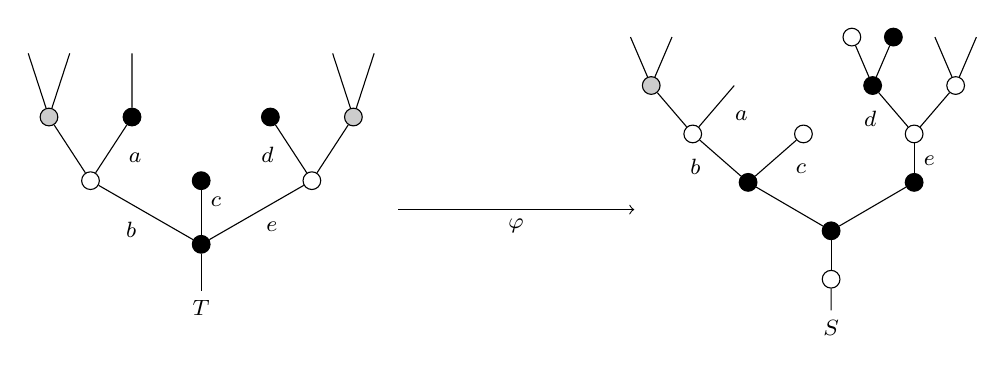
\begin{tikzpicture}[grow=up,auto,level distance=2.3em,
every node/.style = {font=\footnotesize},
dummy/.style={circle,draw,inner sep=0pt,minimum size=2.25mm}]
	\tikzstyle{level 2}=[sibling distance = 4em]
	\tikzstyle{level 3}=[sibling distance = 3em]
	\tikzstyle{level 4}=[sibling distance = 1.5em]
	\node at (0,0.25) {$T$}
		child{node [dummy,fill = black] {}
			child{node [dummy,fill=white] {}
				child{node [dummy,fill = black!20] {}
					child
					child
				}
				child{node [dummy,fill = black] {}
				edge from parent node [near end] {$d$}}
			edge from parent node [swap] {$e$}}
			child{node [dummy,fill=black] {}
			edge from parent node [swap, near end] {$c$}}
			child{node [dummy,fill=white] {}
				child{node [dummy,fill = black] {}
					child
				edge from parent node [swap, near end] {$a\phantom{d}$}}
				child{node [dummy,fill = black!20] {}
					child
					child
				}
			edge from parent node {$b$}}
		};
\begin{scope}[level distance=1.75em]
	\tikzstyle{level 3}=[sibling distance = 6em]
	\tikzstyle{level 4}=[sibling distance = 4em]
	\tikzstyle{level 5}=[sibling distance = 3em]
	\tikzstyle{level 6}=[sibling distance = 1.5em]
	\tikzstyle{level 7}=[sibling distance = 0.75em]
	\node at (8,0) {$S$}
		child{node [dummy,fill = white] {}
			child{node [dummy,fill = black] {}
				child{node [dummy,fill = black] {}
					child{node [dummy,fill=white] {}
						child{node [dummy,fill = white] {}
							child
							child
						}
						child{node [dummy,fill = black] {}
							child{node [dummy,fill=black] {}
						}
							child{node [dummy,fill=white] {}}
						edge from parent node [near end] {$d$}}
					edge from parent node [swap] {$e\phantom{1}$}}
				}
				child{node [dummy,fill = black] {}
					child{node [dummy,fill=white] {}
					edge from parent node [swap, near end] {$c\phantom{1}$}}
					child{node [dummy,fill=white] {}
						child{
						edge from parent node [swap,near end] {$a\phantom{d}$}}
						child{node [dummy,fill = black!20] {}
							child
							child
						}
					edge from parent node [near end] {$\phantom{1}b$}}
				}
			}
		};
\end{scope}
	\draw [->] (2.5,1.5) -- node [swap] {$\varphi$} (5.5,1.5);
\end{tikzpicture}
\end{equation}
\end{example}


\begin{proposition}
One has an identification
\[
\Omega_G^e \simeq 
|\Omega_{G}^{\{+\infty\}_{\langle \bullet \rangle}}|.
\]
\end{proposition}


\begin{proof}
We note first that $\Omega_{G}^e$ contains all label maps that are $\{A,B\}$-inert. In fact, any map of $\Omega_{G}^e$ clearly has a unique factorization as such a label map followed by an underlying planar isomorphism of trees that replaces some of the $X$ and $B$ labels with $A$ labels.
We will refer to the former as label maps and to the latter as relabel maps.

We recall that 
$\Omega_{G}^{\{+\infty\}_{\langle n \rangle}}$
consists of trees with $2n+3$ types of labels: 
$X$-labels, $B$-labels and $2n+1$ distinct types of $A$-labels.
One can equivalently encode such a tree as a string 
$T_0 \to \cdots \to T_n$
of relabel maps. Indeed, the $A$-label nodes of $T_n$ in such a string are partitioned into $2n+1$ types according to that node's labels one the $T_i$ (which are either all $A$'s, some $X$'s and then $A$'s or some $B$'s and then $A$'s).
Moreover, a diagram
\[
\begin{tikzcd}
	T_0 \ar{r} \ar{d}[swap]{f_0} & 
	T_1 \ar{r} \ar{d}[swap]{f_1} & 
	\cdots \ar{r} &
	T_n \ar{d}[swap]{f_n} &
\\
	T'_0 \ar{r} &
	T'_1 \ar{r} &
	\cdots \ar{r} &
	T'_n 
\end{tikzcd}
\]
with $f_i$ label maps of $\Omega^{e}_G$ is then equivalent to a label map $f_n \colon T_n \to T'_n$ respecting all $2n+3$ labels 
in $\Omega_{G}^{\{+\infty\}_{\langle n \rangle}}$.
Since the string description above is also compatible with the simplicial structure maps in the obvious way, 
the result is now clear. 
\end{proof}


Our next task will be that of identifying a convenient Lan-final subcategory $\bar{\Omega}_G^{e} \hookrightarrow \Omega_G^e$.
We first introduce the auxiliary notion of alternating trees.
We recall the notion of input path (Notation \ref{INPUTPATH NOT})
$I(e) = \{f \in T \colon e \leq_d f\}$ for an edge $e \in T$, which naturally extends to $T$ in any of $\in \Omega, \Phi, \Omega_G, \Phi_G$.

\begin{definition}\
A $G$-tree $T \in \Omega_G$ is called \textit{alternating} if, for all leafs $l \in T$ one has that the input path $I(l)$ has an even number of elements.

Further, a vertex $e^{\uparrow} \leq e$ is called \textit{active}
if $|I(e)|$ is odd and \textit{inert} otherwise.

Finally, a tall map $T \xrightarrow{\varphi} T'$ between alternating $G$-trees is called a 
\textit{tall alternating map}
if for any inert vertex $e^{\uparrow} \leq e$ of $T$ one has that 
$T'_{ e^{\uparrow} \leq e)}$ is an inert vertex of $T'$.

We will denote the category of alternating $G$-trees and tall alternating maps by $\Omega_G^a$.
\end{definition}


\begin{example}
Two alternating trees (for $G=\**$ the trivial group) and a planar tall alternating map between them follow, with active nodes in black ($\bullet$) and white nodes in white ($\circ$).
\begin{equation}\label{REGALTERNMAPLR EQ}
\begin{tikzpicture}[grow=up,auto,level distance=2.3em,every node/.style = {font=\footnotesize},dummy/.style={circle,draw,inner sep=0pt,minimum size=1.75mm}]
	\tikzstyle{level 2}=[sibling distance = 4em]
	\tikzstyle{level 3}=[sibling distance = 3em]
	\tikzstyle{level 4}=[sibling distance = 1.5em]
	\node at (0,0.85) {$T$}
		child{node [dummy,fill = black] {}
			child{node [dummy,fill=white] {}
				child{node [dummy,fill = black] {}
					child
					child
				}
				child{node [dummy,fill = black] {}
				edge from parent node [near end] {$d$}}
			edge from parent node [swap] {$e$}}
			child{node [dummy,fill=white] {}
			edge from parent node [swap, near end] {$c$}}
			child{node [dummy,fill=white] {}
				child{node [dummy,fill = black] {}
					child
				edge from parent node [swap, near end] {$a\phantom{d}$}}
				child{node [dummy,fill = black] {}
					child
					child
				}
			edge from parent node {$b$}}
		};
\begin{scope}[level distance=1.75em]
	\tikzstyle{level 3}=[sibling distance = 6em]
	\tikzstyle{level 4}=[sibling distance = 4em]
	\tikzstyle{level 5}=[sibling distance = 3em]
	\tikzstyle{level 6}=[sibling distance = 1.5em]
	\tikzstyle{level 7}=[sibling distance = 0.75em]
	\node at (9,0) {$S$}
		child{node [dummy,fill = black] {}
			child{node [dummy,fill = white] {}
				child{node [dummy,fill = black] {}
					child{node [dummy,fill=white] {}
						child{node [dummy,fill = black] {}
							child
							child
						}
						child{node [dummy,fill = black] {}
							child{node [dummy,fill=white] {}
								child{node [dummy,fill = black] {}}
								child{node [dummy,fill = black] {}}
						}
							child{node [dummy,fill=white] {}}
						edge from parent node [near end] {$d$}}
					edge from parent node [swap] {$e\phantom{1}$}}
				}
				child{node [dummy,fill = black] {}
					child{node [dummy,fill=white] {}
					edge from parent node [swap, near end] {$c\phantom{1}$}}
					child{node [dummy,fill=white] {}
						child{node [dummy,fill = black] {}
							child{node [dummy,fill=white] {}
								child{node [dummy,fill = black] {}
									child
								}
							}
						edge from parent node [swap,near end] {$a\phantom{d}$}}
						child{node [dummy,fill = black] {}
							child
							child
						}
					edge from parent node [near end] {$\phantom{1}b$}}
				}
			}
		};
\end{scope}
	\draw [->] (3,2) -- node [swap] {$\varphi$} (6,2);
\end{tikzpicture}
\end{equation}
The term ``alternating'' comes from the fact that no adjacent nodes have the same color. We note, however, that there is additional restriction: the ``outer'' vertices, i.e. those immediately below a leaf or the one immediately above the root, are necessarily black/active
(not, however, that this does \textit{not} apply to stumps).
%As for the map $\varphi$, we assume additionally that it is a planar map (so that by the tallness condition the root is sent to the root and leaves are sent to leaves while respecting the planar order) and that it sends the labelled edges of $T$ to the eponymous edges of $S$ (though this information is in fact redundant: only one such planar tall alternating map exists).
\end{example}

\begin{remark}
	One can extend Definition \ref{SUBSTITUTIONDATUM} to the alternating context by defining a substitution datum to be alternating if it is given by isomorphisms for inert nodes and by alternating maps for active nodes. It is then straightforward to check that Proposition \ref{SUBDATAUNDERPLAN PROP} and its equivariant analogue Proposition \ref{SUBDATAUNDERPLANG PROP} extend to give alternating analogues.
\end{remark}

\begin{definition}
	$\bar{\Omega}_G^e \hookrightarrow \Omega_G^e$ is the full subcategory of $(B,A,X)$-labeled trees whose underlying trees is alternating, active nodes are labeled by $X$, and passive nodes are labeled by $A$ or $B$. 
\end{definition}

We note that conditions (i) and (ii) in Definition \ref{EXTTREECAT DEF} imply that maps in 
$\bar{\Omega}_G^e$ are underlying alternating maps.

The following establishes the required finality of $\bar{\Omega}_G^e$ in $\Omega_G^e$.

\begin{proposition}\label{LXP PROP}
	For each $U \in \Omega_G^e$ there exists a unique 
	$\mathsf{lr}_X (U) \in \bar{\Omega}_G^e$ together with a unique planar label map of $\Omega_G^e$
	\[\mathsf{lr}_X (U) \to U.\]
	Furthermore, $\mathsf{lr}_X$ extends to a right retraction $\mathsf{lr}_X \colon \Omega_G^e \to \bar{\Omega}_G^e$.
\end{proposition}

\begin{proof}
	Given $U$, we form a collection of outer faces
	$\{U_i^A\} \amalg \{U_j^B\} \amalg \{U_k^X\}$
where the $U_i^A, U_j^b$ are simply the $A,B$-labeled nodes
and the $\{U_k^X\}$ are the maximal outer subtrees whose nodes have only $X$-labels (we note that these may possible be sticks). 
Lemma \ref{OUTERFACEUNION LEM} then guarantees that the $V_G(U_k^{X})$ are disjoint, so that one can apply (the equivariant version of Proposition \ref{BUILDABLE PROP})
to build 
\begin{equation}\label{LRXDEF EQ}
T = \mathsf{lr}(U) \to U
\end{equation}
such that $\{U_{v_{G e}}\} = \{U_i^A\} \amalg \{U_j^B\} \amalg \{U_k^X\}$. $T$ has an obvious $(B,A,X)$-labeling making 
(\ref{LRXDEF EQ}) into a label map, but we must still check $T \in \bar{\Omega}^{e}_G$, i.e. that $T$ is alternating with the $X$-labeled vertices being precisely the $X$-labeled vertices.
Let us now write any input path of $T$ as 
$I(e) = (e = e_n \leq e_{n-1} \leq \cdots \leq e_1 \leq e_0)$.
By Lemma \ref{OUTERFACEUNION LEM} and maximality of the $U_k^X$, no pair of consecutive vertices $v_{Ge_i}$ and $v_{Ge_{i+1}}$ can be both $X$-labeled.
On the other hand, again by Lemma \ref{OUTERFACEUNION LEM} any edge of $U$ belongs to some $U^X_k$ and therefore:
\begin{inparaenum}
	\item[(i)] at least one of in each pair of consecutive vertices $v_{Ge_i}$ and $v_{Ge_{i+1}}$ is $X$-labeled;
	\item[(ii)] if $r \in T$ is a root, $v_{G r}$ is $X$-labeled;
	\item[(iii)] if $l \in T$ is a leaf $v_{G l_{n-1}}$ is $X$-labeled.
\end{inparaenum}
This suffices to conclude $T \in \bar{\Omega}_{G}^e$, and
uniqueness of $T$ is immediate from the uniqueness in Lemma \ref{OUTERFACEUNION LEM}. 


It remains to check that $\mathsf{lr}_X$ in fact defines a functor. We consider the following diagram.
\[
\begin{tikzcd}
	\mathsf{lr}_X(U) \ar{r} \ar[dashed]{d}[swap]{\mathsf{lr}_X(f)} & U \ar{d}{f}
\\
	\mathsf{lr}_X(V) \ar{r} & V
\end{tikzcd}
\]
When $f$ is a root pullback map, we define $\mathsf{lr}_X(f)$ to likewise be a root pullback map. When $f$ is a rooted tall map, writing $T=\mathsf{lr}_X(U)$ one has a map of rooted $T$-substitution data
$\{\mathsf{lr}_X(V_{v_{G_e}})\} \to \{V_{v_{G_e}}\}$,
which after converted to a tree map yields the desired map 
$\mathsf{lr}_X(f)$.
To check that $\mathsf{lr}_X$ respects composition of maps, 
the only non immediate case is that of a root pullback followed by a rooted map, in which case this follows from Remark \ref{PULLCOMP REM}.
\end{proof}


\begin{example}
The following illustrates the $\mathsf{lr}_X$ construction when applied to the map $\varphi$ in (\ref{REGALTERNMAP EQ}).
\begin{equation}
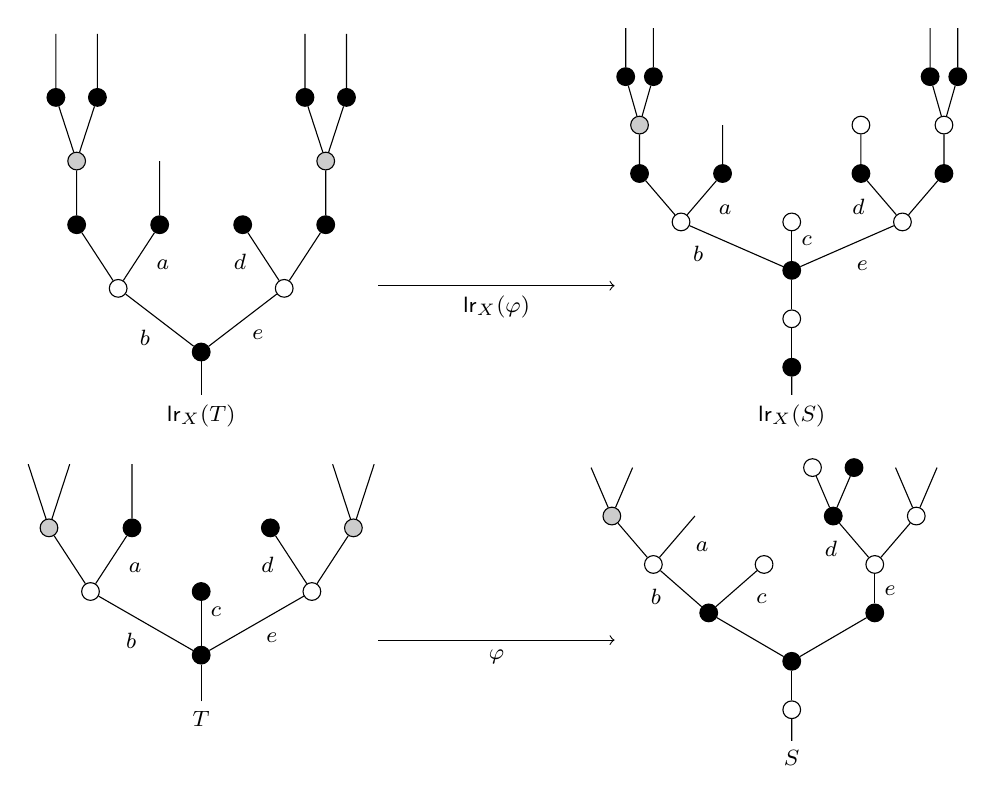
\begin{tikzpicture}[grow=up,auto,level distance=2.3em,
every node/.style = {font=\footnotesize},
dummy/.style={circle,draw,inner sep=0pt,minimum size=2.25mm}]
	\tikzstyle{level 2}=[sibling distance = 6em]
	\tikzstyle{level 3}=[sibling distance = 3em]
	\tikzstyle{level 4}=[sibling distance = 1.5em]
	\node at (0,0.85) {$\mathsf{lr}_X(T)$}
		child{node [dummy,fill = black] {}
			child{node [dummy,fill=white] {}
				child{node [dummy,fill = black] {}
					child{node [dummy,fill = black!20] {}
						child{node [dummy,fill = black] {}
							child}
						child{node [dummy,fill = black] {}
							child}
					}
				}
				child{node [dummy,fill = black] {}
				edge from parent node [near end] {$d$}}
			edge from parent node [swap] {$e$}}
			child{node [dummy,fill=white] {}
				child{node [dummy,fill = black] {}
					child
				edge from parent node [swap, near end] {$a\phantom{d}$}}
				child{node [dummy,fill = black] {}
					child{node [dummy,fill = black!20] {}
						child{node [dummy,fill = black] {}
							child}
						child{node [dummy,fill = black] {}
							child}
					}
				}
			edge from parent node {$b$}}
		};
\begin{scope}
	\tikzstyle{level 2}=[sibling distance = 4em]
	\tikzstyle{level 3}=[sibling distance = 3em]
	\tikzstyle{level 4}=[sibling distance = 1.5em]
	\node at (0,-3) {$T$}
		child{node [dummy,fill = black] {}
			child{node [dummy,fill=white] {}
				child{node [dummy,fill = black!20] {}
					child
					child
				}
				child{node [dummy,fill = black] {}
				edge from parent node [near end] {$d$}}
			edge from parent node [swap] {$e$}}
			child{node [dummy,fill=black] {}
			edge from parent node [swap, near end] {$c$}}
			child{node [dummy,fill=white] {}
				child{node [dummy,fill = black] {}
					child
				edge from parent node [swap, near end] {$a\phantom{d}$}}
				child{node [dummy,fill = black!20] {}
					child
					child
				}
			edge from parent node {$b$}}
		};
\end{scope}
\begin{scope}[level distance=1.75em]
	\tikzstyle{level 3}=[sibling distance = 6em]
	\tikzstyle{level 4}=[sibling distance = 4em]
	\tikzstyle{level 5}=[sibling distance = 3em]
	\tikzstyle{level 6}=[sibling distance = 1.5em]
	\tikzstyle{level 7}=[sibling distance = 1em]
	\node at (7.5,0.85) {$\mathsf{lr}_X(S)$}
		child{node [dummy,fill = black] {}
			child{node [dummy,fill = white] {}
				child{node [dummy,fill = black] {}
					child{node [dummy,fill=white] {}
						child{node [dummy,fill = black] {}
							child{node [dummy,fill = white] {}
								child{node [dummy,fill = black] {}
									child}
								child{node [dummy,fill = black] {}
									child}
							}
						}
						child{node [dummy,fill = black] {}
							child{node [dummy,fill=white] {}}
						edge from parent node [near end] {$d$}}
					edge from parent node [swap] {$e\phantom{1}$}}
					child{node [dummy,fill=white] {}
					edge from parent node [swap, near end] {$c\phantom{1}$}}
					child{node [dummy,fill=white] {}
						child{node [dummy,fill=black] {}
							child
						edge from parent node [swap,near end] {$a\phantom{d}$}}
						child{node [dummy,fill=black] {}
							child{node [dummy,fill = black!20] {}
								child{node [dummy,fill=black] {}
									child
								}
								child{node [dummy,fill=black] {}
									child
								}
							}
						}
					edge from parent node [near end] {$\phantom{1}b$}}
				}
			}
		};
\end{scope}
\begin{scope}[level distance=1.75em]
	\tikzstyle{level 3}=[sibling distance = 6em]
	\tikzstyle{level 4}=[sibling distance = 4em]
	\tikzstyle{level 5}=[sibling distance = 3em]
	\tikzstyle{level 6}=[sibling distance = 1.5em]
	\tikzstyle{level 7}=[sibling distance = 0.75em]
	\node at (7.5,-3.5) {$S$}
		child{node [dummy,fill = white] {}
			child{node [dummy,fill = black] {}
				child{node [dummy,fill = black] {}
					child{node [dummy,fill=white] {}
						child{node [dummy,fill = white] {}
							child
							child
						}
						child{node [dummy,fill = black] {}
							child{node [dummy,fill=black] {}
						}
							child{node [dummy,fill=white] {}}
						edge from parent node [near end] {$d$}}
					edge from parent node [swap] {$e\phantom{1}$}}
				}
				child{node [dummy,fill = black] {}
					child{node [dummy,fill=white] {}
					edge from parent node [swap, near end] {$c\phantom{1}$}}
					child{node [dummy,fill=white] {}
						child{
						edge from parent node [swap,near end] {$a\phantom{d}$}}
						child{node [dummy,fill = black!20] {}
							child
							child
						}
					edge from parent node [near end] {$\phantom{1}b$}}
				}
			}
		};
\end{scope}
	\draw [->] (2.25,2.5) -- node [swap] {$\mathsf{lr}_X(\varphi)$} (5.25,2.5);
	\draw [->] (2.25,-2) -- node [swap] {$\varphi$} (5.25,-2);
\end{tikzpicture}
\end{equation}
\end{example}




\newpage



\section{Model structures}
\label{MODEL_STRUCTURES_SECTION}

Summarizing the results in the previous section, we have that the free $\mathbb F_G$-extension $\P[u]$ defined by the pushout
\begin{equation}\label{CELLEXTPUSH EQ}
\begin{tikzcd}
  \mathbb F_G X \arrow[d, "u"'] \arrow[r] & \P \arrow[d]\\
  \mathbb F_G Y \arrow[r] & \P[u]
\end{tikzcd}
\end{equation}
is given by a left Kan extension along 
$(\bar{\Omega}_{G}^e)^{op} \xrightarrow{\mathsf{lr}} \Sigma_G^{op}$. So as to study the homotopical properties of the map $\P \to \P[u]$ we will identity a suitable filtration of this map, which will in turn be induced by a suitable filtration of the extension tree category $\bar{\Omega}_{G}^e$.


\subsection{Filtration pieces}

First, given $T\in \Omega_G^e$, we write $V_X(T)$ (resp. $V_Y(T)$) to denote the sets of $X$-labeled and $Y$-labeled (non-equivariant) vertices of $T$.
The \textit{degree} of $T \in \bar{\Omega}_{G}^e$,
denoted $|T|$, is defined to be the sum $|T|_X + |T|_Y$, where $|T|_X$, $|T|_Y$ are defined by
\[
|T|_X = \dfrac{|V_X(T)|}{|G r|} = \sum\limits_{G v\in V_{G,X}(T)}\dfrac{|G v|}{|G r|},
\qquad
|T|_Y = \dfrac{|V_Y(T)|}{|G r|} = \sum\limits_{G v\in V_{G,Y}(T)}\dfrac{|G v|}{|G r|}
\]
for $G r$ the root orbit of $T$. 

Intuitively, $|T|_X$ counts the number of $X$-labeled vertices in each individual tree component of $T$.


\begin{remark}
	One of the key properties of the degrees just defined is that they are invariant under root pullback.
\end{remark}


\begin{definition}\label{TREE_FILTRATION_PIECES_DEFINITION}
We define subcategories of $\bar{\Omega}_{G}^e$:
  \begin{itemize}
  \item $\bar{\Omega}_G^e[\leq k]$ (resp. $\Omega_G^e[k]$) is the full subcategory of trees 
  $T \in \bar{\Omega}_G^e$ with $|T|\leq k$ (resp. $|T| = k$);
  \item $\bar{\Omega}_G^e[\leq k,-]$ (resp. $\bar{\Omega}_G^e[k,-]$) is the full subcategory of $\bar{\Omega}_G^e[\leq k]$ (resp. $\bar{\Omega}_G^e[k]$) of trees $T$ with $|T|_{Y}\neq k$;
  \item $\bar{\Omega}_G^e[k,0]$ is the full subcategory of 
  $\bar{\Omega}_G^e[k]$ of trees $T$ with $|T|_X = 0$ (or, equivalently, $|T|_{Y} = k$).
%  \item If $\Xi$ is any of the above categories, and $C\in \Sigma_G$, let $\Xi(C)$ denote the full subcategory of $\Xi$ spanned by those trees $T$ with $val(T) \simeq C$.
  \end{itemize}
The above definitions still hold if we replace $\bar\Omega_G^e$ with $\Omega_G^a$; in particular, we have vertical forgetful functors
\[
\begin{tikzcd}
  \bar\Omega_G^e[k,-] \arrow[dr, "\mathsf{fgt}"'] \arrow[rr, hookrightarrow] && \bar\Omega_G^e[k] \arrow[dl, "\mathsf{fgt}"]\\
  & \Omega_G^a[k]
\end{tikzcd}
\]
\end{definition}


\begin{remark}\label{LIMMOR REM}
  The categories $\bar{\Omega}_G^e[k]$ and $\bar{\Omega}_G^e[k,-]$ have only rather limited morphisms.
  In fact, all maps in these categories must be underlying quotients of trees. Indeed, it is clear from Definition \ref{EXTTREECAT DEF} that maps never lower degree and, moreover, degree is preserved iff $\mathcal{P}$-vertices are substituted by $\mathcal{P}$-vertices (rather than larger trees in $\bar{\Omega}_G^e$, which would necessarily possess $X$-vertices).
  
  Moreover, we have a clear isomorphism of categories $\bar\Omega_G^e[k,0] \simeq \Omega_G^a[k]$. 
\end{remark}


\begin{lemma}\label{MINUS_LAN_FINAL_LEMMA}
  $\bar{\Omega}_G^e[\leq k-1]$ is $\mathsf{Ran}$-initial in $\bar{\Omega}_G^{e}[\leq k,-]$ over $\Sigma_G$.
\end{lemma}

In the proof we will make use of the following construction on 
$\Omega_{G}^e$: given $T \in \Omega_{G}^e$ we will let $T_{\mathcal{P}}$ denote the result of replacing all $X$-labeled nodes of $T$ with $\mathcal{P}$-labeled nodes.

\begin{remark}\label{YINERT REM}
  Unlike the $\mathsf{lr}_{\mathcal{P}}$ construction of Proposition \ref{LXP PROP}, which defines a functor 
  $\mathsf{lr}_{\mathcal{P}} \colon
  \Omega_G^e \to \bar{\Omega}_G^e $,
  the construction 
  $(\minus)_{\mathcal{P}}$ does not define a full functor
  $\Omega_G^e \to \Omega_G^e$, instead being functorial, and the obvious maps $T_{\mathcal{P}} \to T$ natural, only with respect to the $Y$-inert maps of $\Omega_G^e$.
\end{remark}


\begin{example}
%  We observe that this construction is symmetric across all tree components, and hence, to give an example, it suffices to show want happens on a single component (i.e. when $G = \set{e}$).
Combining the $(\minus)_{\mathcal{P}}$ and $\mathsf{lr}_{\mathcal{P}}$ constructions one obtains a construction sending trees in $\bar{\Omega}^e_G$ to trees in $\bar{\Omega}^e_G$.
We illustrate this for the tree $T \in \bar{\Omega}^e_G$ below, where black nodes are $\P$-labeled, white nodes are $X$-labeled, and grey nodes are $Y$-labeled.
\[
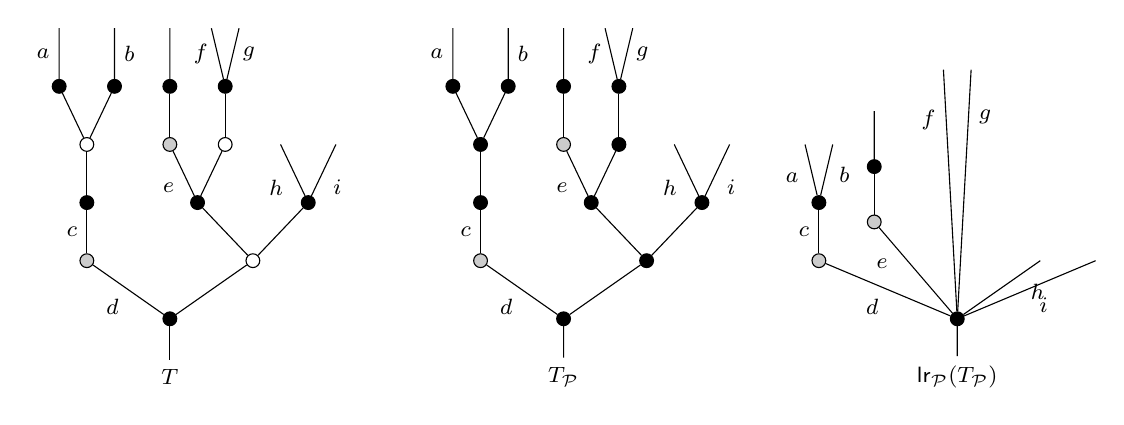
\begin{tikzpicture}
  [grow=up,auto,level distance=2.1em,every node/.style = {font=\footnotesize},dummy/.style={circle,draw,inner sep=0pt,minimum size=1.75mm}]
  % [grow=up, level distance = .8cm, auto, every node/.style={font=\small}, dummy/.style={circle,draw,inner sep=0.4mm, minimum size=2.25}]
  \tikzstyle{level 2}=[sibling distance=6em]
  \tikzstyle{level 3}=[sibling distance=4em]
  \tikzstyle{level 4}=[sibling distance=2em]
  \tikzstyle{level 5}=[sibling distance=2em]
  \tikzstyle{level 6}=[sibling distance=1em]
  \node{$T$}
  child{node [dummy, fill=black] {}%
    child{node [dummy, fill=white] {}%
      child{node [dummy,fill=black] {}%
        child{edge from parent node [swap] {$i$}}
        child{edge from parent node {$h$}}
      }
      child{node [dummy, fill=black] {}%
        child{node [dummy, fill=white] {}%
          child{node [dummy, fill=black] {}%
            child{edge from parent node [right]{$g$}} 
            child{edge from parent node [left]{$f$}} 
          }
        }
        child{node [dummy, fill=black!20] {}%
          child{node [dummy, fill=black] {}%
            child{}
          }
          edge from parent node {$e$}
        }
      }
    }
    child{node [dummy, fill=black!20] {}%
      child{node [dummy, fill=black] {}%
        child{node [dummy, fill=white] {}%
          child{node [dummy, fill=black] {}%
            child{edge from parent node [swap] {$b$}}
          }
          child{node [dummy, fill=black] {}%
            child{edge from parent node {$a$}}
          }
        }
        edge from parent node {$c$}
      }
      edge from parent node {$d$}
    }
  };
  \node at (5,0){$T_{\mathcal{P}}$}
  child{node [dummy, fill=black] {}%
    child{node [dummy, fill=black] {}%
      child{node [dummy,fill=black] {}%
        child{edge from parent node [swap] {$i$}}
        child{edge from parent node {$h$}}
      }
      child{node [dummy, fill=black] {}%
        child{node [dummy, fill=black] {}%
          child{node [dummy, fill=black] {}%
            child{edge from parent node [right]{$g$}} 
            child{edge from parent node [left]{$f$}} 
          }
        }
        child{node [dummy, fill=black!20] {}%
          child{node [dummy, fill=black] {}%
            child{}
          }
          edge from parent node {$e$}
        }
      }
    }
    child{node [dummy, fill=black!20] {}%
      child{node [dummy, fill=black] {}%
        child{node [dummy, fill=black] {}%
          child{node [dummy, fill=black] {}%
            child{edge from parent node [swap] {$b$}}%
          }
          child{node [dummy, fill=black] {}%
            child{edge from parent node {$a$}}%
          }
        }
        edge from parent node {$c$}
      }
      edge from parent node {$d$}
    }
  };
  \tikzstyle{level 2}=[sibling distance=2em]
  \tikzstyle{level 4}=[sibling distance=1em]
  \node at (10,0){$\mathsf{lr}_{\mathcal{P}}(T_{\mathcal{P}})$}
  child{node [dummy,fill=black] {}%
    child{edge from parent node [swap]{$i$}}
    child{edge from parent node [swap,near end] {$h$}}
    child[sibling distance=1em, level distance = 9em]{edge from parent node [swap, very near end]{$g$}}
    child[sibling distance=1em, level distance = 9em]{edge from parent node [very near end]{$f$}}
    child[level distance = 3.5em]{node [dummy, fill=black!20] {}%
      child[level distance = 2em]{node [dummy, fill=black] {}%
        child{}
      }
      edge from parent node [near end]{$e$}
    }
    child{node [dummy, fill=black!20] {}%
      child{node [dummy, fill=black] {}%
        child{edge from parent node [swap,near end]{$b$}}
        child{edge from parent node [near end] {$\phantom{b}a$}}
        edge from parent node {$c$}
      }
      edge from parent node {$d$}
    }
  };    
\end{tikzpicture}
\]
\end{example} 


\begin{proof}[Proof of Lemma \ref{MINUS_LAN_FINAL_LEMMA}]
Just as in the proof of Lemma \ref{LANPULLCOMA LEM}, for each 
$C \in \Sigma_G$, 
the under categories
$C \downarrow \bar{\Omega}_G^e[\leq k-1]$,
$C \downarrow \bar{\Omega}_G^e[\leq k,-]$
have initial subcategories 
$C \downarrow_{\mathsf{r},\simeq} \bar{\Omega}_G^e[\leq k-1]$.
$C \downarrow_{\mathsf{r},\simeq} \bar{\Omega}_G^e[\leq k,-]$
of those objects
$(S,q \colon C \to \mathsf{lr}(S))$ such that 
$q$ is an ordered isomorphism on roots,
and thus an isomorphism in $\Sigma_G$.

It now suffices to show (cf. (\cite[X.3.1]{McL})) that for each
$(S,q \colon C \to \mathsf{lr}(S))$ in 
$C \downarrow_{\mathsf{r},\simeq} \bar{\Omega}_G^e[\leq k,-]$
the undercategory
\begin{equation}\label{UNDERCATPR EQ}
	(S,q) \downarrow  
	(C \downarrow_{\mathsf{r},\simeq} \bar{\Omega}_G^e[\leq k-1])
\end{equation}
is non-empty and connected. 
Moreover, we note that an object in 
(\ref{UNDERCATPR EQ})
is uniquely encoded by a map $T \to S$ inducing a rooted isomorphism on $\mathsf{lr}$.

The case $S\in \Omega_G^e[\leq k-1]$ is immediate. 
Otherwise, since $|S|_Y \neq k$ it is
$|\mathsf{lr}_{\mathcal{P}}(S_{\mathcal{P}})|<k$
and the map 
$\mathsf{lr}_{\mathcal{P}}(S_{\mathcal{P}}) \to S$,
which is a rooted isomorphism on $\mathsf{lr}$, shows that
(\ref{UNDERCATPR EQ}) is indeed non-empty.

  
Otherwise, given any rooted tall map $T \to S$ with 
$T \in \bar{\Omega}_G^e[k-1]$ (which gives a rooted isomorphism on $\mathsf{lr}$ and thus encodes a unique object of (\ref{UNDERCATPR EQ})). One can then form a diagram
\begin{equation}\label{K-1LANFINAL EQ}
\begin{tikzcd}
	      & S & \mathsf{lr}_{\mathcal{P}}(S_{\mathcal{P}}) \ar{l}
\\
	T \ar{ur} \ar{r} & T' \ar{u}[swap]{Y-\text{inert}} & \mathsf{lr}_{\mathcal{P}}(T'_{\mathcal{P}}) \ar{l} \ar{u}
\end{tikzcd}
\end{equation}
where $T \to T' \to S$ is the natural factorization such that the second map is $Y$-inert, i.e., $T'$ is obtained from $T$ by simply relabeling to $X$ those $Y$-labeled vertices of $T$ that become $X$-vertices in $S$. Note that the existence of the right square in (\ref{K-1LANFINAL EQ}) follows from the map $T' \to S$ being $Y$-inert together with Remark \ref{YINERT REM}.
Since (\ref{K-1LANFINAL EQ}) becomes a diagram of rooted  isomorphism on $\mathsf{lr}$, if produces the necessary zigzag connecting the objects $T \to S$ and 
$\mathsf{lr}_{\mathcal{P}}(S_{\mathcal{P}}) \to S$
in (\ref{UNDERCATPR EQ}), finishing the proof.
%
%
%Further, given any other element
%\begin{equation}
%    \label{K-1_LAN_FINAL_EQ2}
%    \begin{tikzcd}
%      val(S) && val(T) \arrow[ll, "f"']\\
%      & C \arrow{ur}[swap]{q_S} \arrow[ul, "q_T"]
%    \end{tikzcd}
%  \end{equation}
%  in the overcategory, consider the following zig-zag of maps connecting the objects (\ref{K-1_LAN_FINAL_EQ1}) and (\ref{K-1_LAN_FINAL_EQ2}):
%\begin{equation}\label{K-1_LAN_FINAL_DIAGRAM}
%\begin{tikzcd}
%	&& S &&
%\\[20pt]
%	&& \tilde q_T^*(S) \arrow[u, "\tilde q_T"'] &&
%\\
%	S^\wedge_\P \arrow[uurr, "\partial_\P"] &
%	\tilde q_T^*(S^\wedge_\P) \arrow[l, "\tilde q_T"'] \arrow[ur, "\partial_\P"] \arrow[rr, "\partial_\P"] &&
%	 T' \arrow[ul, "\partial_\P"'] & T \arrow[l, "\partial_Y"'] \arrow[uull, "f"']
%\\[20pt]
%	&& C \arrow[ull, "q_S"] \arrow[ul, "q_T"'] \arrow[ur, "q_T"] \arrow[urr, "q_T"'] 
%\end{tikzcd}
%\end{equation}
%  Here, we have omitted the notation ``$val$'' from the top three rows. To understand this diagram, we first record that we have a factorization:
%  \[
%  q_S = \tilde q_T q_T,
%  \]
%  Then, if we let $C_S = val(S) = val(S^\wedge_\P)$ and $C_T = val(T)$, we have
%  \[
%  C \xrightarrow{q_T} C_T \xrightarrow{\tilde q_T} C_S
%  \]
%  and hence, by the unique factorization of maps in $\Omega_{G,e}$, a factorization% via Remark \ref{OMEGA_E_REMARKS} (2), a factorization
%  \[
%  \begin{tikzcd}
%    C_T \arrow[d, "\tilde q_T"'] \arrow[r, dashed] & \tilde q_T^*(S^\wedge_\P) \arrow[d, dashed, "\tilde q_T"]\\
%    C_S \arrow[r] & S^\wedge_\P
%  \end{tikzcd}
%  \]
%  (where we are recording $C \to val(S)$ as a planar-tall map $C \to S$). 
%  A similar analysis shows that the top left trapezoid commutes. 
%
%  The other regions also commute by a straightforward analysis. Indeed, the top right trapezoid commutes by unique factorization, and finally the middle triangle of $\partial_\P$ maps commutes since $(\tilde q_T^*S)^\wedge_\P = \tilde q^*_T(S^\wedge_\P)$. 
%  
%  Lastly, we must check that the middle two maps are in fact elements of the appropriate overcategory. This follows from the fact that $S^\wedge_\P$ and $T$ have $|-|_Y < k$. Thus, the overcategory in question is connected, as desired.
\end{proof}


Similarly to the $(\minus)_{\mathcal{P}}$ construction,
there is also a construction $T_Y$ which replaces all $X$-labels of $T \in \Omega_G^e$ with $Y$-labels. Moreover, in this case the construction restricts directly to a construction on 
$\bar{\Omega}_G^e$,
which is easily seen to be functorial (and the $T_Y \to T$ maps natural) with regards to $\mathcal{P}$-inert maps. Remark \ref{LIMMOR REM} thus implies that 
$(\minus)_Y \colon \bar{\Omega}_G^e[k] \to 
\bar{\Omega}_G^e[k,0]$
is a left retraction, 
resulting in the following.
\begin{lemma}
  \label{ZERO_LAN_FINALITY_LEMMA}
  $\bar{\Omega}_G^{e}[k,0]$ is $\mathsf{Ran}$-initial in $\bar{\Omega}_G^e[k]$ over $\Sigma_G$.
\end{lemma}

%\begin{proof}[Proof of Lemma \ref{ZERO_LAN_FINALITY_LEMMA}]
%  This follows analogously to Lemma \ref{MINUS_LAN_FINAL_LEMMA}, by replacing Diagram \ref{K-1_LAN_FINAL_DIAGRAM} with the diagram below:
%  \[
%  \begin{tikzcd}
%    && S & \\[20pt]
%    &&\tilde q_T^*(S) \arrow[u, "\tilde q_T"]\\
%    S^\wedge_Y \arrow[uurr, "\partial_Y"] && \tilde q_T^*(S^\wedge_Y) \arrow[ll, "\tilde q_T"'] \arrow[u, "\partial_Y"] \arrow[rr, "\partial_Y"] && T \arrow[ull, "\partial_Y"'] \arrow[uull, "f"']\\
%    && C \arrow[ull, "q_S"] \arrow[u, "q_T"] \arrow[urr, "q_T"'] 
%  \end{tikzcd}
%  \]
%\end{proof}


In what follows we write $N^e \colon \Omega_G^{e,op} \to \mathcal{V}$ for the functor in (\ref{FREEEXTUSEFCOLNEW EQ}),
and abuse notation by likewise writing $N^e$ for any of its restrictions to the subcategories in 
Definition \ref{TREE_FILTRATION_PIECES_DEFINITION}.

We are now in a position to produce the desired filtration of the map $\mathcal{P} \to \mathcal{P}[u]$ in 
(\ref{CELLEXTPUSH EQ}).

\begin{definition}
  \label{PK_DEFN}
  Let $\P_k$ denote the left Kan extension
\[
\begin{tikzcd}
	|[alias=U]| \bar{\Omega}_G^e[\leq k]^{op} \arrow[r, "N^e"] \arrow[d, "\mathsf{lr}"'] & \V
\\
	\Sigma_G^{op} \arrow[ur, "\P_k"', ""{name=V}]
	\arrow[Rightarrow, from=U, to=V]
\end{tikzcd}
\]
\end{definition}
Noting that $\bar{\Omega}_G^e[\leq 0] \simeq \Sigma_G$ (since $|T|=0$ only if $T$ is a $G$-corolla with $\mathcal{P}$-labeled vertex) and that $\bar{\Omega}_G^e$
is the union of (the nerves of) the 
$\bar{\Omega}_G^e[\leq k]$, one has a filtration
\begin{equation}\label{FILT EQ}
	\mathcal{P} = 
	\mathcal{P}_0 \to 
	\mathcal{P}_1 \to
	\mathcal{P}_2 \to
	\cdots \to 
	\colim_k \mathcal{P}_k = \mathcal{P}[u].
\end{equation}


To analyze (\ref{FILT EQ}) homotopically we will further make use of a pushout description of each individual map 
$\mathcal{P}_{k-1} \to \mathcal{P}_k$. To do so, we note that the diagram of inclusions
\begin{equation}\label{INCDIAG EQ}
\begin{tikzcd}
	\bar{\Omega}_G^{e}[k,-] \arrow[d] \arrow[r] &
	\bar{\Omega}_G^{e}[\leq k,-] \arrow[d]
\\
	\bar{\Omega}_G^e[k] \arrow[r] &
	\bar{\Omega}_G^e[\leq k]
\end{tikzcd}
\end{equation}
is a pushout of at the level of nerves.
Indeed, this follows since
\[
\bar{\Omega}_G^e[k] \cap 
\bar{\Omega}_G^{e}[\leq k,-]
= \bar{\Omega}_G^{e}[k,-],
	\qquad
\bar{\Omega}_G^e[k] \cup 
\bar{\Omega}_G^{e}[\leq k,-]
= \bar{\Omega}_G^{e}[\leq k],
\]
and since a map $T \to S$ in 
$\bar{\Omega}_G^e[\leq k]$
will be in one of subcategories in (\ref{INCDIAG EQ}) iff $T$ is.

Since Lemma \ref{MINUS_LAN_FINAL_LEMMA} provides an identification 
$\Lan_{\bar{\Omega}_{G,e}[\leq k,-]^{op}}N^e \simeq
\Lan_{\bar{\Omega}_{G,e}[\leq k-1]^{op}}N^e = \mathcal{P}_{k-1}$,
applying left Kan extensions to (\ref{INCDIAG EQ}) yields the pushout diagram below.
\begin{equation}\label{FILTRATION_LAN_SQUARE_DIAGRAM}
\begin{tikzcd}
	\Lan_{\bar{\Omega}_{G}^e[k,-]^{op}}N^e \arrow[d] \arrow[r] & 
	\P_{k-1} \arrow[d]
\\
	\Lan_{\bar{\Omega}_{G}^e[k]^{op}}N^e \arrow[r] &
	\P_k
\end{tikzcd}
\end{equation}

We will find it convenient for our purposes to 
have explicit levelwise descriptions for 
(\ref{FILTRATION_LAN_SQUARE_DIAGRAM}),
which we now describe.



%Finally, we show that each layer $\Omega_G^e[\leq k]$ can be built from $\Omega_{G}^e[\leq k-1]$ via a pushout which attaches trees with precise degree $k$. 
%While dealing with general pushouts of categories requires solving a ``word problem'' on morphisms, we will only work in cases where the problem collapses. We recall that, given a square of categories
%\[
%\begin{tikzcd}
%  \mathcal A \arrow[d] \arrow[r] & \mathcal C \arrow[d]\\
%  \mathcal C \arrow[r] & \mathcal D
%\end{tikzcd}
%\]
%if the nerve of this square is a pushout in $\sSet$, then this is a pushout of categories (since the nerve is the inclusion of a reflective subcategory).


%If we further assume that the span of functors is built out of fully-faithful inclusions, these pushouts behave as nicely as possible with left Kan extensions.
%\begin{lemma}
%  \label{LAN_PUSHOUT_LEMMA}
%  Given any diagram in categories of the form 
%\[
%\begin{tikzcd}
%  \mathcal A \arrow[d] \arrow[r, "f"] & \mathcal C \arrow[d, %"i"]\\
%  \mathcal B \arrow[r, "g"] & \mathcal D \arrow[r, "Y"] \arrow[d, "j"] & \V \\
%  & \mathcal D
%\end{tikzcd}
%\]
%such that the square is a nerve pushout of fully-faithful %functors, then $\Lan_j Y$ is the pushout of the induced span
%\[
%\begin{tikzcd}
%  \Lan_{j i f}(Y i f) \arrow[r] \arrow[d] & \Lan_{j i}(Y i)\\
%  \Lan_{j g}(Y g).
%\end{tikzcd}
%\]
%\end{lemma}
%\begin{proof}
%  By the universal property of left Kan extensions, it suffices to show that, for any functor $Z: \V \to \D$, the natural map
%  \[
%  \V^\D(Y, Z j) \longto \V^{\mathcal B} (Y g, Z j g) \prod\limits_{\V^{\mathcal A}(Y i f, Z j i f)} \V^{\mathcal C}(Y i, Z j i)
%  \]
%  is a bijection. These two sets give the same data: a collection of maps $\Phi_b: Y(b) \to Z(b)$ and $\Phi_c:Y(c) \to Z(c)$ for all $b\in \mathcal B$ and $c \in \mathcal C$, such that $\Phi_b = \Phi_c$ whenever $b = c \in \mathcal A$. In general, the compatibilites required on the right are less demanding. However, with the above assumptions, a map $d \to d'$ in $\mathcal D$ is \textit{uniquely} a map in $\mathcal A$, $\mathcal B \setminus \mathcal A$, or $\mathcal C \setminus \mathcal A$, and thus all the necessary compatibilities are covered by (at least) one of the $\set{\Phi_b}$ or $\set{\Phi_c}$. 
%\end{proof}

\begin{proposition}
For each level $C\in \Sigma_G$,
(\ref{FILTRATION_LAN_SQUARE_DIAGRAM})
is given by the following pushout in $\V^{\mathsf{Aut}(C)}$
\begin{equation}\label{FILTRATION_LAN_LEVEL}
\begin{tikzcd}
	\coprod\limits_{[T] \in \mathsf{Iso}
		\left(C \downarrow_{\mathsf{r}} \Omega_G^a[k]\right)}
	\left(
		\bigotimes\limits_{v \in V_{G}^{ac}(T)}\P(T_v) \otimes
		Q_T^{in}[u]
	\right)
		\mathop{\otimes}\limits_{\mathsf{Aut}(T)} \mathsf{Aut}(C)
	\arrow[r] \arrow[d] &
	\P_{k-1}(C) \arrow[d] 
\\
	\coprod\limits_{[T] \in \mathsf{Iso}
		\left(C \downarrow_{\mathsf{r}} \Omega_G^a[k]\right)}
	\left(
		\bigotimes\limits_{v \in V_{G}^{ac}(T)}\P(T_v) \otimes
		\bigotimes\limits_{v \in V_{G}^{in}(T)} Y(T_v)
	\right)
		\underset{\mathsf{Aut}(T)}{\otimes} \mathsf{Aut}(C)
	\arrow[r] &
	\P_k(C)
\end{tikzcd}
\end{equation}
where $\Omega_G^a[k]$ denotes alternating trees with exactly $k$ 
passive vertices, $ V_{G}^{ac}(T)$, $V_{G}^{in}(T)$ denote the active and passive vertices of $T$,
and $Q_T^{in}[u]$ is the domain 
of the the iterated pushout product
\[
		\underset{v \in V_G^{in}(T)}
		{\mathlarger{\mathlarger{\mathlarger{\square}}}}u(T_v)
	\colon
		Q_T^{in}[u] \to
		\bigotimes\limits_{v \in V_{G}^{in}(T)} Y(T_v).
\]
%where the left vertical map is the iterated pushout product
%\[
%\coprod \mathop{\square}\limits_{V_{G,\P}(T)}\iota_{\P(T_v)}\mathop{\square} [u]^{\square \mathbb V_{G,in}(T)},
%\]
%$\iota_{\P(T_v)}$ is the canonical map $\varnothing \to \P(T_v)$ out of the initial object, and $\Omega_G^a[k](C)$ is as in Definition \ref{TREE_FILTRATION_PIECES_DEFINITION}.
\end{proposition}


\begin{proof}
We first note that, following 
Definition \ref{LIMMOR REM}, both 
$\bar{\Omega}_{G}^e[k]^{op}$ and $\bar{\Omega}_{G}^e[k,-]^{op}$
are split Grothendieck constructions over
$\Omega_G^a[k]^{op}$.
The fibers of these Grothendieck constructions
are the cube and punctured cube categories
\[
	(X \to Y)^{\times V_G^{in}(T)},
\qquad
	(X \to Y)^{\times V_G^{in}(T)} - Y^{\times V_G^{in}(T)}
\]
and thus by computing the left Kan extensions on the leftmost map in (\ref{FILTRATION_LAN_SQUARE_DIAGRAM}) iteratively by first left Kan extending to $\Omega_G^a$, we can rewrite that map as
\begin{equation}\label{FILTINTALT EQ}
	\Lan_{\Omega_G^a[k]^{op}}
	\left(
		\bigotimes\limits_{v \in V_{G}^{ac}(T)}\P(T_v) \otimes
		\underset{v \in V_{G}^{in}(T)}
		{\mathlarger{\mathlarger{\mathlarger{\square}}}}
		u(T_v)
	\right).
\end{equation}
The desired description of the leftmost map given in (\ref{FILTRATION_LAN_LEVEL})
now follows by noting that the root undercategories
$C \downarrow_{\mathsf{r}} \Omega_G^a[k]$
are groupoids.
\end{proof}


 
\subsection{Existence of (semi) model structures} 
\todo[inline]{replaced $\backslash$ F with $\mathcal F$ (as opposed to $\mathbb F$)} 
\renewcommand{\F}{\ensuremath{\mathcal F}} 

In order to encode the homotopical information inspired by $N_\infty$-operads dicussed in the introduction, we will introduce (semi) model structures on the categories $\Op_G(\V)$ and $\Op^G(\V)$ for a wide range of $\V$. 

We begin by describing general notions of projective model structures on diagram categories.

\begin{definition}[\cite{Ste16}]
  Let $\Pi$ be a finite group, and $\F$ a collection of subgroups. A map $f$ is called an \textit{$\F$-fibration} (resp. \textit{$\F$-weak equivalence}) if $f^H$ is so in $\V$ for all $H\in \F$, or an \textit{$\F$-cofibrations} if it has lifts against all maps which are both $\F$-fibrations and $\F$-weak equivalences. The \textit{$\F$-model structure} on $\V^\Pi$, if it exists, is the unique model structure with $\F$-fibration, $\F$-weak equivalences, and $\F$-cofibrations.
\end{definition}

\begin{definition}
  \label{SUBD_PROJ_F_MODEL_STRUCTURE}
  Now suppose we are given a small category $\mathcal D$, a subcategory $\mathcal D' \subseteq \mathcal D$, and a collection $\F_d$ of subgroups of $\mathrm{Aut}(d)$ for each $d\in \mathcal D'$.
 We define the \textit{$\mathcal D'$-projective model structure} on $\V^{\mathcal D}$, if it exists, to be the unique model structure where $f$ is a fibrations (resp. weak equivalence) iff $f(d)$ is so in $\V^{\mathrm{Aut}(d)}_{\F_d}$ for all $d\in \mathcal D'$. 

Equivalently, this is the model structure transfered, via the technology of Kan \cite[11.6.1]{Hi03} or Schwede-Shipley \cite[2.3]{SS00} along either composite of adjunctions
  \[
  \begin{tikzcd}
    \V^{\mathcal D}_{\mathcal D',\F} \arrow[d, shift right] \arrow[r, shift right, "i^*"'] & \V^{\mathcal D'}_{\F} \arrow[l, shift right, "i_!"'] \arrow[d, shift right]\\
    \V^{\mathrm{Ob}(\mathcal D)}_{\mathcal D',\F} \arrow[r, shift right, "i^*"'] \arrow[u, shift right] & \V^{\mathrm{Ob}(\mathcal D')}_{\F} \arrow[l, shift right] \arrow[u, shift right]
  \end{tikzcd}
  \]
  where we give
  \begin{itemize}
  \item $\V^{\mathrm{Ob}(\mathcal D')}_{\F} = \mathop{\prod}\limits_{d\in \mathcal D'}\V^{\mathrm{Aut}(d)}_{\F_d}$ the level $\F_d$-model structure, if it exists, and
  \item $\V^{\mathrm{Ob}(\mathcal D)}_{\mathcal D',\F}$ the transfered model structure from $\V^{\mathrm{Ob}(\mathcal D')}_{\F}$.
  \end{itemize}
  
  If each $\F_d$ is the set of all subgroups of $\mathrm{Aut}(d)$, we refer to the above as the $\mathcal D'$-projective \textit{genuine} model structure. 

  If $\mathcal D' = \mathcal D$, we refer to the above as simply the \textit{projective $\F$-model structure}.
\end{definition}

\begin{remark}
  \label{LEVEL_COFIB_REMARK}
  We record that for any cofibration $f$ in $\V^{\mathcal D}_{\mathcal D', \F}$, $f(d)$ is a cofibration in $\V^{\mathrm{Aut}(d)}_{\F_d}$ for all $d\in \mathcal D'$. Indeed, the map
  \[
  \mathcal D(d,c) \cdot_{\mathrm{Aut}(d)}(-): \V^{\mathrm{Aut}(d)}_{gen} \to \V^{\mathrm{Aut}(c)}_{gen}
  \]
  sends generating cofibrations to disjoint unions of generating cofibrations.
\end{remark}

\begin{definition}
  We say $\V$ is \textit{admissible for finite groups} if, for any finite group $\Pi$ and collection of subgroups $\F$, the $\F$ model structure $\V^\Pi_\F$ exists.

  In particular, this will hold if $\V$ has \textit{cellular fixed points} (see \ref{CELL DEF}). 
\end{definition}

{\color{blue}
To prove the existence of semi model structures, we will require our base category $\V$ to be sufficiently nice:
\begin{definition}
  \label{STRONGLY_CELLULAR}
  We say a category $\V$ is \textit{strongly cellular} if the following hold: 
  \begin{enumerate} 
  \item $\V$ is a strongly cofibrantly-generated symmetric monoidal model category,
  \item $\V$ has cellular fixed points,
  \item $\V$ has cofibrant symmetric pushout powers (see Definition \ref{COFSYMPUSHPOW}).
  \end{enumerate} 
\end{definition} 
To upgrade these to Quillen model structures, we need additional assumptions:
\begin{definition}
  \label{UNDERLYING_STRONGLY_CELLULAR}
  We say a category $\V$ is \textit{underlying strongly cellular} if $\V$ is strongly cellular and additionally
  \begin{enumerate}
  \item gennuine cofibrations in $\V^\Pi$ are underlying cofibrations in $\V$ for all finite groups $\Pi$, and
  \item every object in $\V$ is cofibrant.
  \end{enumerate}
\end{definition}
}

\begin{notation}
  We will use $\Sigma_\F$ to denote a (fixed) full subcategory of $\Sigma_G$ (later, we will show this is equivalent to a collection $\F = \set{\F_n}$ of sets $\F_n$ of graph subgroups of $G\times \Sigma_n$), and we let $\Sym_\F(\V)$ denote the presheaf category $\V^{\Sigma_\F^{op}}$. 
  Additionally, we write $\Sym_G^\F(\V)$ for the category $\Sym_G(\V)$ endowed with the $\Sigma_\F$-projective genuine model structure from Definition \ref{SUBD_PROJ_F_MODEL_STRUCTURE} (equivalently, this is the model structure transfered from $\Sym_\F(\V)$).
\end{notation}



\subsubsection{Genuine $G$-Operads}
\label{OP_G_EXISTS_SECTION}
%\subsubsection{The $\F$-model structures}

In this section, we prove Theorem \ref{MAINEXIST2 THM} in two parts: Corollary \ref{OP_F_SEMI_MODEL_THM} and Theorem \ref{OP_F_Q_MODEL_THM}.

Fixing a subcategory $\Sigma_\F$, we identify the following maps of $\Op_G(\V)$.
\begin{definition} 
  We say a map $f: \O \to \P$ in $\Op_G(\V)$ is an  
  \begin{itemize} 
  \item[(i)] \textit{$\F$-fibration} (resp. $\F$-weak equivalence) if $f(C):\O(C) \to \P(C)$ is one in $\V^{\mathrm{Aut}(C)}_{gen}$ for all $\F$-admissible $G$-corollas $C\in\Sigma_\F$. 
  \item[(ii)] \textit{$\F$-cofibration} if it has the left lifting property against all maps which are both $\F$-fibrations and $\F$-weak equivalences. 
  \item[(iii)] \textit{$\Sigma_\F$-cofibration} if $f$ is an cofibration in $\Sym_G^\F(\V)$. 
  \item[(iv)] \textit{level genuine cofibration} if $f(C)$ is a cofibration in $\V^{\mathrm{Aut}(C)}_{gen}$ for all $C\in \Sigma_\G$. 
  \end{itemize} 
\end{definition} 

% In particular, $\P\in \V\Op_G$ will be called \textit{$\F$-cofibrant} if $\varnothing \to \P$ is an $\F$-cofibration. 

\begin{definition} 
  The \textit{$\F$-(semi) model structure} on $\Op_G(\V)$, if it exists, is the unique (semi) model structure with $\F$-fibrations, $\F$-weak equivalences, and $\F$-cofibrations. Equivalently, it is the transfered (semi) model structure along the adjoints 
  \[ 
  \begin{tikzcd} 
    \Op_G(\V) \arrow[r, shift right, "\mathsf{fgt}"'] & \Sym_G^\F(\V) \arrow[l, shift right, "\mathbb F_G"']
  \end{tikzcd} 
  \] 
\end{definition} 

Using general arguments of \cite{SS00}, this structure would be cofibrantly generated, with generating arrows 
\begin{align*} 
  I_\F &= \sets{\mathbb F_G(\Sigma_G(-,C) \cdot i)}{C \in \Sigma_\F,\ i\in I}\\ 
  J_\F &= \sets{\mathbb F_G(\Sigma_G(-,C) \cdot j)}{C \in \Sigma_\F,\ j\in J}, 
\end{align*} 
for $I$ (resp. $J$) the generating (trivial) cofibrations of $\V$. 

\begin{notation} 
  If $\Sigma_\F = \Sigma_G$, we refer to the $\F$-model structure as the \textit{genuine} model structure. 
\end{notation} 

\begin{remark}
        \label{GENUINE_FGTRIGHT_REMARK} 
  We record the following standard facts (generalized in \ref{FGTRIGHT PROP}, \ref{FGTLEFT PROP}, and \ref{EXTERINTADJ EQ}):
  \begin{itemize}
  \item [(i)] if $\phi: \Pi \to \bar \Pi$ is a homomorphism of groups, then both the induction map and the forgetful functor 
  \[ 
  \phi_!: \bar\Pi\cdot_\Pi(-): \V^\Pi_{gen} \leftrightarrows \V^{\bar \Pi}_{gen}: \phi^*
  \] 
  are left Quillen for the genuine model structures. 
  \item[(ii)] The symmetric monoidal product extends to a left Quillen functor
          \[
          \V^\Pi_{gen} \times \V^{\bar \Pi}_{gen} \to \V^{\Pi \times \bar\Pi}_{gen}.
          \]
  \end{itemize}
\end{remark} 

\begin{theorem}\label{OP_G_SEMI_MODEL_THM} 
  The genuine semi model structure on $\Op_G(\V)$ exists for all Cartesian strongly cellular $\V$.
\end{theorem} 

The key technical result follows as an easy corollary of the simple case of a result from Section \ref{COFIB SEC}.

\begin{proposition}
\label{GENUINE_TREE_BOX_COFIBRANT_PROP} 
  Suppose $\V$ is Cartesian strongly cellular, $T\in \Omega_G^a$, and we are given level genuine cofibrations $f_{ac}: \mathcal Q \to \P$ and $f_{in}: X \to Y$ in $\Sym_G(\V)$. Then the iterated box product
  \[ 
  f^{\Box V_G(T)} = \mathop{\Box}\limits_{[v] \in V_G^{ac}(T)} f_{ac}([v]) \Box \mathop{\Box}\limits_{[v]\in V_G^{in}(T)}f_{in}([v]) 
  % f^{\Box V_G(T)} = \mathop{\Box}\limits_{Gv \in V_G(T)} f(Gv) 
  \] 
  is a cofibration in $\V^{\mathrm{Aut}(T)}_{gen}$.  
\end{proposition}
\begin{proof}
        Given $[v]\in V_G(T)$, let $\llbracket v \rrbracket$ denote the orbit in $V_G(T)/\mathsf{Aut(T)}$. Then we have a natural group homomorphism
        \[ 
        \beta: \mathsf{Aut}(T) \to \prod\limits_{\llbracket v \rrbracket} \Sigma_{|\llbracket v \rrbracket |} \wr \mathsf{Aut}(T_{[v]})
        \]
        and the forgetful functor 
        \[
        \beta^*: V^{\Pi \Sigma_{\llbracket v \rrbracket} \wr \mathsf{Aut}(T_{[v]})} \to \V^{\mathsf{Aut}(T)}
        \]
        preserves genuine cofibrations. Thus, it suffices to show that $f^{\Box V_G(T)}$ is cofibrant on the right hand side. This follows immediately by Proposition \ref{POWERF PROP} and Remark \ref{GENUINE_FGTRIGHT_REMARK}.
        % \[
        % \prod \V^{\mathsf{Aut}(T_{[v]})}_{gen} \to \V^{\Sigma_{|\llbracket v \rrbracket|} \wr \mathsf{Aut}(T_{[v]})}
        % \]
        % is left Quillen, and by inspection, 
        % \[
        % \prod_i \V^{G_i}_{gen} \to \V^{\prod G_i}_{gen}
        % \]
        % is left Quillen, completing the proof.
  %%%%%%%%%%%%%%%%%%%% OLD PROOF       (c.f. the proof of Proposition \ref{AUTTCOFPUSH PROP})
  % \todo[inline]{This result isn't actually a particular case of loc cite; or the precise statement of a family version.}
  % Using grafting composition $T \simeq C \circ (T^1_1, \ldots, T^{k_1}_1, T^1_2, \ldots, T^{k_r}_r)$, we go by induction on $|V_G(T)|$. The base cases of $|V_G(T)| = 0$ or 1 are trivial. Now, we note that we have a decomposition 

  % \[ 
  % f^{\Box V_G(T)} = f([v_r]) \Box \mathop{\Box}\limits_{i=1}^r\left( \left( f^{\Box V_G(T_i)} \right) ^{\Box k_i} \right) 
  % \] 

  % where $[v_r]$ is the root orbit. We will build this map in stages, preserving cofibrancy in each step. 

  % \begin{itemize} 
  % \item By induction, for each $i$, $f^{\Box V_G(T_i)}$ is a cofibration in $\V^{\mathrm{Aut}(T_i)}_{gen}$. 
  % \item By Proposition \ref{POWERF PROP}, each $\left( f^{\Box V_G(T_i)} \right)^{\Box k_i}$ is a cofibration in $\V^{\Sigma_{k_i}\wr \mathrm{Aut}(T_i)}_{gen}$. 
  % \item By Remark \ref{EXTERINTADJ EQ}, $\mathop{\Box}\limits_{i=1}^r\left(\left( f^{\Box V_G(T_i)} \right)^{\Box k_i}\right)$ is a cofibration in $\V^{\Pi \Sigma_{k_i} \wr \mathrm{Aut}(T_i)}_{gen}$. 
  % \item By Proposition \ref{FGTLEFT PROP}, $f([v_r])$ is a cofibration in $\V^{\mathrm{Aut}(T)}_{gen}$. 
  % \item Finally, by the decomposotion of $\mathrm{Aut}(T)$ and Proposition \ref{BIQUILLENG PROP}, we have the full $f^{\Box V_G(T)}$ is a cofibration in $\V^{\mathrm{Aut}(T)}_{gen}$, as desired. 
  % \end{itemize} 

  % If any $f([v])$ were trivial, then, during the appropriate step above, the resulting box product would again be trivial, by the same referenced results. 
\end{proof} 

\begin{corollary}\label{CELLULAR_LEVEL_COFIB_PROP} 
  For $\V$ Cartesian strongly cellular, and for any free $\mathbb F_G$-extension  
  \[ 
  \begin{tikzcd} 
    \mathbb F_G X \arrow[d, "u"'] \arrow[r] & \P \arrow[d]\\ 
    \mathbb F_G Y \arrow[r] & \P[u] 
  \end{tikzcd} 
  \] 
  where $u: X \to Y$ is a level genuine cofibration and $\P$ is level genuine cofibrant in $\Sym_G(\V)$, $\P \to \P[u]$ is a level cofibration, trivial if $u$ is so. 
\end{corollary}  
\begin{proof} 
  By using the levelwise filtration from (\ref{FILTRATION_LAN_LEVEL}), this follows immediately from Proposition \ref{GENUINE_TREE_BOX_COFIBRANT_PROP} and Remark \ref{GENUINE_FGTRIGHT_REMARK}. 
\end{proof} 


\begin{proof}[Proof of Theorem \ref{OP_G_SEMI_MODEL_THM}] 
  Using \cite[Lemma 2.3]{SS00}, the fact that weak equivalences and transfinite compositions are levelwise implies that Corollary \ref{CELLULAR_LEVEL_COFIB_PROP} and Remark \ref{LEVEL_COFIB_REMARK} are sufficient.
\end{proof} 

Somewhat surprisingly, the existance of the $\F$-semi-model structures follows identically as the genuine. Indeed, \ref{LEVEL_COFIB_REMARK} also implies that cofibrations in $\Sym_G^\F(\V)$ are in fact level genuine cofibrations, which suffices.
\begin{corollary} 
  \label{OP_F_SEMI_MODEL_THM}
  For any full subcategory $\Sigma_\F \subseteq \Sigma_G$, the $\F$-semi-model structure on $\Op_G(\V)$ exists if $\V$ is Cartesian strongly cellular. \qed
\end{corollary} 


Moreover, if our base category $\V$ is sufficiently nice, these semi model structures are in fact Quillen model structures. 
\begin{theorem} 
  \label{OP_F_Q_MODEL_THM}
  If $\V$ is Cartesian underlying strongly cellular, % and moreover
  % \begin{itemize}
  % \item genuine cofibrations in $\V^\Pi$ are underlying cofibrations in $\V$ for all finite groups $\Pi$, and
  % \item every object in $\V$ is cofibrant,
  % \end{itemize}
  then the $\F$-model structure $\Op_G^\F(\V)$ exists for any $\Sigma_\F$.
\end{theorem} 
\begin{proof} 
  In these cases, the technical hypotheses on $\P$ needed for Corollary \ref{CELLULAR_LEVEL_COFIB_PROP} are always satisfied. 
\end{proof} 

\begin{example} 
  The $\F$-model structure exists on $\s\Op_G$ for any $G$-vertex family $\F$. 
\end{example} 

\todo[inline]{come back}

% \newpage
\subsubsection{$G$-Operads}
\label{G_OP_EXISTS_SECTION}

We now turn our consideration back to regular $G$-operads $\O \in \Op^G(\V)$, and again split our proof of Theorem \ref{MAINEXIST1 THM} into two parts, Corollary \ref{F_OP_SEMI_MODEL_THM} and Theorem \ref{F_OP_Q_MODEL_THM}.

Now, we let $\F = \set{\F_n}$ denote any collection of sets $\F_n$ of subgroups, closed under conjugation, of $G\times \Sigma_n$.

\begin{definition}
  The \textit{$\F$-model structure} on $\Sym^G(\V)$ is the model category
\[
\Sym^G_\F(G) := \prod\limits_n \V^{G\times \Sigma_n}_{\F_n}.
\]
%If $\F$ is the complete $G$-vertex system, this will be refered to as the \textit{genuine} model structure.
\end{definition}

We identify the following maps in $\Op^G(\V)$.
\begin{definition}
  \label{F_MAPS_DEFINITION}
  Suppose $\V$ is cofibrantly generated and admissible for finite groups. A map $f: \O \to \P$ in $\Op^G(\V)$ is called a
  \begin{itemize}
  \item \textit{$\F$-fibration} (resp. $\F$-weak equivalence) if for all $n$, $f(n): \O(n) \to \P(n)$ is one in $\V^{G \times \Sigma_n}_{\F_n}$; that is, $f(n)^\Lambda$ is a fibration (resp weak equivalence) in $\V$ for all $\Lambda \in \F_n$.
  \item \textit{$\F$-cofibration} if it has the left lifting property against all map which are both $\F$-fibrations and $\F$-weak equivalences. 
  \item \textit{level $\F$-cofibration} if $f(n)$ is a cofibration in $\V^{G\times \Sigma_n}_{\F_n}$ for all $n$.
  \end{itemize}
\end{definition}

\begin{definition}
  The \textit{$\F$-(semi) model structure} is the unique (semi) model structure on $\Op^G(\V)$, if it exists, with $\F$-fibrations, $\F$-cofibrations, and $\F$-weak equivalences. 
%If $\F$ is the complete $G$-vertex family, we call this the \textit{genuine} model structure on $\V\Op^G$.
\end{definition}
Equivalently, the $\F$-model structure is the unique transfered structure across the adjunction
\[
\begin{tikzcd}
  \Op^G_\F(\V) \leftrightarrows \prod \V^{G \times \Sigma_n}_{\F_n}.
\end{tikzcd}
\]
Again, the machinery of \cite{SS00} says the right hand side has generating (trivial) cofibrations
\begin{align*}
  I_\F &= \sets{G \times \Sigma(-,n)/\Gamma \cdot i}{i \in I}\\
  J_\F &= \sets{G \times \Sigma(-,n)/\Gamma \cdot j}{j \in J}
\end{align*}
so $\Op^G_\F(\V)$ would have generating cofibrations $\mathbb F I_\F = \sets{\mathbb F (i_\F)}{i_\F\in I_\F}$, and similarly for trivial cofibrations.


\begin{theorem}
  \label{G_OP_SEMI_MODEL_THM}
  The genuine semi-model structure on $\Op^G(\V)$ exists whenever $\V$ is Cartesian strongly cellular.
\end{theorem}

The key technical result is an easy particular case of the stronger \ref{AUTTCOFPUSH PROP}.
\begin{proposition}
\label{AUTTCOFPUSH_GEN_PROP} 
  Suppose $\V$ is Cartesian strongly cellular, $T\in \Omega^a$, and we are given level genuine cofibrations $f_{ac}: Q \to \P$ and $f_{in}: X \to Y$ in  $\Sym^G(\V)$. Then the iterated box product 
  \[ 
  f^{\Box V(T)} = \mathop{\Box}\limits_{v \in V_{ac}(T)} f_{ac}(v) \Box \mathop{\Box}\limits_{v\in V_{in}(T)}f_{in}(v) 
  \] 
  is a cofibration in $\V^{G\times \Sigma_T}_{gen}$.
\end{proposition}

\begin{corollary}\label{CELLULAR_LEVEL_COFIB_PROP2} 
  For $\V$ Cartesian strongly cellular, and for any free $\mathbb F$-extension  
  \[ 
  \begin{tikzcd} 
    \mathbb F X \arrow[d, "u"'] \arrow[r] & \P \arrow[d]\\ 
    \mathbb F Y \arrow[r] & \P[u] 
  \end{tikzcd} 
  \] 
  where $u: X \to Y$ is a level genuine cofibration and $\P$ is level genuine cofibrant in $\Sym^G(\V)$, $\P \to \P[u]$ is a level cofibration, trivial if $u$ is so. 
\end{corollary}  
\begin{proof} 
  As $\Op(\V^G) = \Op^G(V)$, we consider the filtration in (\ref{FILTRATION_LAN_LEVEL}) with $G = *$ and $\V = \V^G$ . Then the result follows from Proposition \ref{AUTTCOFPUSH_GEN_PROP} and Remark \ref{FGTRIGHT PROP}.
\end{proof} 

\begin{proof}[Proof of Theorem \ref{G_OP_SEMI_MODEL_THM}]
  Follows exactly as \ref{OP_G_SEMI_MODEL_THM}, replacing \ref{CELLULAR_LEVEL_COFIB_PROP} with \ref{CELLULAR_LEVEL_COFIB_PROP2}.  
\end{proof}

% \begin{remark}
%   It also follows in a more complicated fashion. 

%   We note that if $u: X \to Y$ is a genuine cofibration in $\V^{G\times \Sigma}_\F$, then $i_! u$ is certainly a genuine level cofibration in $\V^{\Sigma_G^{op}}$. Further, by Lemma \ref{SYM_QUI_ADJ}, $\P$ level cofibrant implies $i_*\P$ level cofibrant, so by Corollary \ref{CELLULAR_LEVEL_COFIB_PROP}, $i_*\P \to (i_*\P)[u]$ is a level genuine trivial cofibration. Lastly, since $\mathbb F \simeq i^*\mathbb F_G i_!$, and $i^*$ preserves both pushouts and cofibrations, the result follows.
% \end{remark}

\begin{remark}
  The Cartesian condition can be dropped from the above theorem. Indeed, when restricting the machinery of Section \ref{GENUINE_OP_MONAD_SECTION} to $G = *$ and $\V = \V^G$, Remark \ref{NEED_WREATH_REMARK} no longer applies, and hence we may reformulate the monad on spans from Definition \ref{WSPAN_MONAD_DEFINITION} by replacing $\Fin$ with $\Fin_{\mathsf{Iso}}$ and using the natural map $\mathsf F_{\mathsf{Iso}} \wr \V^{op} \xrightarrow{\otimes} \V^{op}$ for \textit{any} symmetric monoidal product $\otimes$ on $\V$.
\end{remark}

Again, the $\F$-model structures also follows from \ref{CELLULAR_LEVEL_COFIB_PROP}, as level (trivial) $\F$-cofibrations are also level (trivial) genuine cofibrations.
\begin{corollary} 
  \label{F_OP_SEMI_MODEL_THM}
  For any $G$-vertex system $\F$, the $\F$-semi-model structure on $\V\Op^G$ exists whenever $\V$ is strongly cellular. \qed
\end{corollary} 
% \begin{proof} 
%   It suffices to show that if $u: X\to Y$ is a level trivial $\F$-cofibration and $\P$ is level $\F$-cofibrant in $\V^{G \times \Sigma}$, then the cellular extension $\P \to \P[u]$ is a level trivial $\F$-cofibration. However, such $u$ are level genuine cofibrations, and such $\P$ are level genuine cofibrant, and hence $\P \to \P[u]$ is a level trivial genuine cofibration by said corollary, and thus is a level trivial $\F$-cofibration. 
% \end{proof} 


As before, this extends to a Quillen model structure if $\V$ is sufficiently nice:
\begin{theorem}
  \label{F_OP_Q_MODEL_THM}
  If $\V$ is Cartesian underlying strongly cellular with cofibrant symmetric pushout powers,% , satisfies the conditions in Theorem \ref{GENUINE_OP_Q_MODEL_THM}, 
then the $\F$-model structure exists on $\Op^G(\V)$. \qed
\end{theorem}

\begin{example}
  The $\F$-model structure exists on $\sOp^G$ for any $G$-vertex system $\F$.
\end{example}


\newpage



\section{Cofibrancy and Quillen equivalences}\label{COFIB SEC}



The key ingredient required to prove our desired Quillen equivalence
\[
	\iota^{\**} \colon
	\mathsf{Op}_G \rightleftarrows \mathsf{Op}^G
	\colon \iota_{\**}
\]
will be an analysis of cofibrant objects in $\mathsf{Op}_G$, which we now provide.


\subsection{Families of subgroups}


This section establishes some useful properties of the model structures associated to families of subgroups. Throughout all groups will be assumed finite.


\begin{definition}\label{FAMILY DEF}
	A \textit{family} $\mathcal{F}$ of subgroups of $G$ is a collection of subgroups 
	$H \leq G$ such that
	\begin{itemize}
	\item if $H \in \mathcal{F}$ then 
	$H^g = gHg^{-1} \in \mathcal{F}$ for all $g \in G$;
	\item if $K \leq H$ and $H \in \mathcal{F}$ then
	$K \in \mathcal{F}$.
	\end{itemize} 
\end{definition}

\begin{remark}\label{SIEVE REM}
	Any family determines a full subcategory 
	$\mathsf{O}_{\mathcal{F}} \hookrightarrow \mathsf{O}_G$
	of those orbital $G$-sets $G/H$ for 
	$H \in \mathcal{F}$.
	
	Moreover, $\mathsf{O}_{\mathcal{F}}$ is a sieve, i.e., for any map $G/K \to G/H$ in $\mathsf{O}_G$ such that $G/H \in \mathsf{O}_{\mathcal{F}}$ it is also $G/K \in \mathsf{O}_{\mathcal{F}}$. In fact, it is easy to check that families are in bijection with sieves.
\end{remark}


\begin{remark}
For fixed $G$ families form a lattice, ordered by inclusion, 
with meet and join given by intersection and union.
\end{remark}


We now recall the following basic notion and result concerning model structures induced by families (cf. \cite[Prop. 2.6]{Ste16}).


\begin{definition}\label{CELL DEF}
	We say a model category $\mathcal{V}$ has 
	\textit{cellular fixed points} if for all finite groups $G$ and subgroups $H,K\leq G$ one has that:
\begin{itemize}
	\item[(i)] fixed points $(\minus)^H \colon \mathcal{V}^G \to \mathcal{V}$ preserve direct colimits;
	\item[(ii)] fixed points $(\minus)^H$ preserve pushouts where one leg is $(G/K)\cdot f$, for $f$ a cofibration;
	\item[(iii)] for each object $X \in \mathcal{V}$, the natural map 
	$(G/K)^H \cdot X \to ((G/K) \cdot X)^H$
	is an isomorphism.
\end{itemize}
\end{definition}


\begin{proposition}\label{FMODELEXIST PROP}
	If $\mathcal{V}$ is a cofibrantly generated model category with cellular fixed points, then for any finite group $G$ and family $\mathcal{F}$, there is a model structure $\mathcal{V}^G_{\mathcal{F}}$ on the category 
	$\mathcal{V}^G$, called the 
	\emph{$\mathcal{F}$-model structure}
	such that both weak equivalences and fibrations are determined by the fixed points $(\minus)^H$ for 
	$H \in \mathcal{F}$.
\end{proposition}

When $\mathcal{F}$ is the family of all subgroups the model structure in Proposition \ref{FMODELEXIST PROP} is called simply the \textit{$G$-genuine model structure}.

We will find it convenient to strengthen the cellularity conditions in Definition \ref{CELL DEF}.


\begin{proposition}\label{STRONGCELL PROP}
	Suppose that $\mathcal{V}$ is a cofibrantly generated model category with cellular fixed points. Then:
	\begin{itemize}
		\item[(i)] $(\minus)^H \colon \mathcal{V}^G \to \mathcal{V}$ preserves cofibrations and pushouts where one leg
			 is a genuine cofibration;
		\item[(ii)] if $X$ is $G$-genuine cofibrant the map 
			$(G/K)^H \cdot X^H \to (G \cdot_K X)^H$ is an isomorphism.
	\end{itemize}
Suppose additionally that $\mathcal{V}$ is a 
closed monoidal model category
as well as strongly cofibrantly generated
(i.e. that the domains of the generating (trivial) cofibrations are cofibrant). Then:
	\begin{itemize}
		\item[(iii)] for $f,g$ genuine cofibrations between genuine cofibrant objects the natural map 
\[f^H \square g^H \xrightarrow{\simeq} (f \square g)^H\]
 is an isomorphism.
 In particular, $X^H \otimes Y^H \xrightarrow{\simeq} 
 (X \otimes Y)^H$ is an isomorphism when $X,Y$ are genuine cofibrant.
	\end{itemize}
\end{proposition}


\begin{proof}
Since all conditions are compatible with retracts, we are free to assume each cofibration $f\colon X \to Y$
(or, for $Y$ cofibrant, the map $\emptyset \to Y$)
is a transfinite composition
\begin{equation}\label{TRANSFCOMP EQ}
	X_0 \xrightarrow{f_0} 
	X_1 \xrightarrow{f_1}
	X_2 \xrightarrow{f_2}
	X_3 \xrightarrow{f_3} 
	\cdots
	\to Y = X_{\beta} = \colim_{\alpha < \beta} X_{\alpha}
\end{equation}
where each $f_{\alpha} \colon X_{\alpha} \to X_{\alpha+1}$
is the pushout of a generating cofibration
$(G/H) \cdot i_{\alpha}$. Both (i) and (ii) now follow by transfinite induction on $\alpha$ in the partial composite map
$X_0 \to X_{\alpha}$, with the successor ordinal case following by Def. \ref{CELL DEF} (ii), (iii) and the limit ordinal case by
Def. \ref{CELL DEF} (i). We note that (ii) also includes an obvious base case $X_0=\emptyset$.
To prove (iii), we consider first the case of $g$ a generating cofibration. The exact same induction argument now applies to any $f$ as in (\ref{TRANSFCOMP EQ}), contingently on a base case $f=(\emptyset \to X)$. But this base case now follows by the exact same argument, now contingent on the base case $f=(\emptyset \to \emptyset)$, which is obvious.
The general case now follows by repeating the same argument, now using the analogous filtration (\ref{TRANSFCOMP EQ}) for $g$.
\end{proof}


We end this section by cataloging some straightforward interactions of $\mathcal{F}$-model structures
with regards to change of group and pushout products.


\begin{proposition}\label{FGTRIGHT PROP}
	Let $\phi \colon G \to \bar{G}$ be a homomorphism and $\mathcal{V}$ be cofibrantly generated with cellular fixed points.	
	Then the adjunction
\begin{equation}
\begin{tikzcd}
	\bar{G}\cdot_G(\minus)
	\colon
	\mathcal{V}^{G}_{\mathcal{F}} \ar[shift left=1]{r}
&
	\mathcal{V}^{\bar{G}}_{\bar{\mathcal{F}}}
	\colon \ar[shift left=1]{l}
	\mathsf{fgt}
\end{tikzcd}
\end{equation}
is a Quillen adjunction if for any 
$H \in \mathcal{F}$ it is $\phi(H) \in \bar{\mathcal{F}}$.
\end{proposition}

\begin{proof}
Since one has a canonical isomorphism of fixed points
$\left(\mathsf{fgt}(X)\right)^H \simeq X^{\phi(H)}$,
it is immediate that the right adjoint preserves fibrations and trivial fibrations.
\end{proof}


\begin{proposition}\label{FGTLEFT PROP}
	Let $\phi \colon G \to \bar{G}$ be a homomorphism and $\mathcal{V}$ be cofibrantly generated with cellular fixed points.		
	Then the adjunction
\begin{equation}
\begin{tikzcd}
	\mathsf{fgt}
	\colon
	\mathcal{V}^{\bar{G}}_{\mathcal{\bar{F}}} \ar[shift left=1]{r}
&
	\mathcal{V}^{G}_{\mathcal{F}}
	\colon
	\mathsf{Hom}_G(\bar{G},\minus)
	\colon \ar[shift left=1]{l}
\end{tikzcd}
\end{equation}
is a Quillen adjunction if for any 
$H \in \bar{\mathcal{F}}$ it is 
$\phi^{-1}(H) \in \mathcal{F}$.
\end{proposition}


\begin{proof}
	Since the double coset formula yields that that
\[
	\mathsf{fgt}\left(\bar{G}/H \cdot f\right)
		\simeq 
	\mathsf{fgt}\left(\bar{G}/H\right) \cdot f
		\simeq
	\left(
		\coprod_{[a] \in \phi(G)\backslash \bar{G} /H}
		{G/\phi^{-1}(H^{a})}
	\right)	\cdot f
\]
it is immediate that the left adjoint $\mathsf{fgt}$ preserves cofibrations and trivial cofibrations.
\end{proof}


Propositions \ref{FGTRIGHT PROP} and \ref{FGTLEFT PROP}
motivate the following definition.

\begin{definition}
	Let $\phi \colon G \to \bar{G}$ be a homomorphism and $\mathcal{F}$ and $\bar{\mathcal{F}}$ families in $G$
	and $\bar{G}$. We define
\begin{align}\label{PHISTARDEF EQ}
	\phi^{\**}(\bar{\mathcal{F}})
		=&
	\{H \leq G : \phi(H) \in \bar{\mathcal{F}}\}
\\
	\phi_!(\mathcal{F})
		=&
	\{\phi(H)^{\bar{g}}\leq \bar{G} : \bar{g} \in \bar{G}, H \in \mathcal{F}\}
\\ \label{PHISTARDEF3 EQ}
	\phi_{\**}(\mathcal{F})
		=&
	\{\bar{H} \leq \bar{G} : 
	\forall_{\bar{g} \in \bar{G}} 
	\left(
	\phi^{-1}(\bar{H}^{\bar{g}}) \in \mathcal{F}
	\right)\}
\end{align}
\end{definition}

\begin{lemma}
The $\phi^{\**}(\bar{\mathcal{F}})$, $\phi_{!}(\mathcal{F})$, $\phi_{\**}(\mathcal{F})$ just defined are 
themselves families. Furthermore
\begin{itemize}
\item[(i)] The ``if'' condition in Proposition \ref{FGTRIGHT PROP} holds iff 
$\mathcal{F} \subset \phi^{\**} (\bar{\mathcal{F}})$
iff
$\phi_{!}(\mathcal{F}) \subset \bar{\mathcal{F}}$.
\item [(ii)]
The ``if'' condition in Proposition \ref{FGTLEFT PROP} holds iff 
$\phi^{\**} (\bar{\mathcal{F}}) \subset \mathcal{F}$
iff
$\bar{\mathcal{F}} \subset \phi_{\**}(\mathcal{F})$.
\end{itemize}
\end{lemma}


\begin{proof}
	Since the result is elementary, we include only the proof of the second iff in (ii), which is the hardest step and illustrates the necessary arguments. This follows by the following equivalences.
\[
	\phi^{\**} (\bar{\mathcal{F}}) \subset \mathcal{F}
\Leftrightarrow
	\left( \underset{ \substack{H \leq G \\ \phi(H) \in \bar{\mathcal{F}} }}{\mathlarger{\mathlarger{\forall}}} 
	H \in \mathcal{F} \right)
\Leftrightarrow
	\left( \underset{\bar{H} \in \bar{\mathcal{F}}}{\mathlarger{\mathlarger{\forall}}}
	\phi^{-1}(\bar{H}) \in \mathcal{F}
	\right)
\Leftrightarrow
	\left( \underset{ \substack{\bar{H} \in \bar{\mathcal{F}}\\\bar{g} \in \bar{G}}}{\mathlarger{\mathlarger{\forall}}}
	\phi^{-1}(\bar{H}^{\bar{g}}) \in \mathcal{F}
	\right)
\Leftrightarrow
        \bar{\mathcal F} \subset \phi_{\**}(\mathcal F)
% 	\phi^{\**} (\bar{\mathcal{F}}) \subset \mathcal{F}
\]
Note that the second equivalence follows since 
$H \leq \phi^{-1}(\phi(H))$ and $\mathcal{F}$ is closed under subgroups while the third equivalence follows since 
$\bar{\mathcal{F}}$ is closed under conjugation. 
\end{proof}


\begin{proposition}\label{BIQUILLENG PROP}
	Suppose that $\mathcal{V}$ is cofibrantly generated, has cellular fixed points, and is also a closed monoidal model category. 	
	Then the bifunctor
\begin{equation}\label{BIQUILLENG EQ}
	\mathcal{V}^G_{\mathcal{F}}
		\times
	\mathcal{V}^G_{\bar{\mathcal{F}}}
		\xrightarrow{\otimes}
	\mathcal{V}^G_{\mathcal{F} \cap \bar{\mathcal{F}}}
\end{equation}
	is a left Quillen bifunctor.
\end{proposition}


\begin{proof}
	The double coset formula now yields
\begin{equation}
	\left(G/H \cdot f\right) \square \left(G/\bar{H} \cdot g\right)
		\simeq
	\left(G/H \times G/\bar{H}\right) \cdot \left(f \square g\right)
		\simeq
	\left(
		\coprod_{[a]\in H \backslash G /\bar{H}}
		{G/H\cap \bar{H}^a} \cdot (f \square g)
	\right)
\end{equation}
and hence the result follows since families are closed under conjugation and subgroups.
\end{proof}


\begin{definition}\label{EXTERINT DEF}
Let $\mathcal{F}$ and $\bar{\mathcal{F}}$ be families in $G$ and $G$, respectively.

We define their \textit{external intersection} to be the 
family of $G \times \bar{G}$ given by
\[
	\mathcal{F} \sqcap \bar{\mathcal{F}}
=
	(\pi_{G})^{\**} (\mathcal{F}) 
		\cap
	(\pi_{\bar{G}})^{\**} (\bar{\mathcal{F}})
\]
for 
$\pi_G \colon G \times \bar{G} \to G$,
$\pi_{\bar{G}} \colon G \times \bar{G} \to \bar{G}$
the projections.
\end{definition}


\begin{remark}
	Combining Proposition \ref{FGTLEFT PROP} 
	with Propositon \ref{BIQUILLENG PROP} yields that
	the following composite is a left Quillen bifunctor.
\begin{equation}\label{EXTERINTADJ EQ}
	\mathcal{V}^{G}_{\mathcal{F}}
		\times
	\mathcal{V}^{\bar{G}}_{\bar{\mathcal{F}}}
		\xrightarrow{\mathsf{fgt}}
	\mathcal{V}^{G \times \bar{G}}_{
	(\pi_G)^{\**}(\mathcal{F})}
		\times
	\mathcal{V}^{G \times \bar{G}}_{
	(\pi_{\bar{G}})^{\**}(\bar{\mathcal{F}})}
		\xrightarrow{\otimes}
	\mathcal{V}^{G \times \bar{G}}_{
	\mathcal{F} \sqcap \bar{\mathcal{F}}}
\end{equation}
\end{remark}


\subsection{Pushout powers}


That (\ref{EXTERINTADJ EQ}) is a left Quillen bifunctor (and its obvious higher order analogues) is one of the key properties of pushout products of $\mathcal{F}$ cofibrations when those cofibrations (and the group) are allowed to change. However, when those cofibrations (and hence $G$) coincide there is an additional symmetric group action that  we will need to consider.

To handle such actions we introduce the following notion.

\begin{definition}\label{COFSYMPUSHPOW}
	We say a monoidal model category $\mathcal{V}$ has 
	\textit{cofibrant symmetric pushout powers}
	if for each cofibration (resp. trivial cofibration) $f$ the pushout product 
	$f^{\square n}$ is a genuine $\Sigma_n$-cofibration (resp. trivial cofibration).
\end{definition}


\begin{remark}
When $\mathcal{V}$ is cofibrantly generated
the condition in Definition \ref{COFSYMPUSHPOW} needs only be checked for generating cofibrations. 
However, the argument needed is somewhat harder than usual due to $(-)^{\square n}$ not preserving composition of maps:
one instead follows the argument in the proof of 
Proposition \ref{POWERF PROP} below when $G=\**$.
\end{remark}


%\begin{remark}
%	Alternatively, we could also have insisted that $f^{\square n}$ be a trivial cofibration if $f$ is. However, while this holds in the examples of interest, it is usually not as helpful from a technical standpoint. Indeed, the main role of pushout powers $f^{\square n}$ is to help study powers $f^{\otimes n}$, but it is often easier to first check directly that $f^{\otimes n}$ is a weak equivalence, and then argue that so is
%$f^{\square n}$ using $2$-out-of-$3$ and the filtration in 
%the proof of Proposition \ref{POWERF PROP}.
%\end{remark}


We now turn to describing the symmetric power analogue of 
Definition \ref{EXTERINT DEF}.

We start with some notation. Letting 
$\lambda$ be a partition 
$E = \lambda_1 \amalg\cdots \amalg \lambda_k$
of a finite set $E$, 
we write 
 $\Sigma_{\lambda} = \Sigma_{\lambda_1} \times \cdots \times
 \Sigma_{\lambda_k} \leq \Sigma_E$ for the subgroup of permutations preserving $\lambda$. 
 In addition, given any $e \in E$ we write
$\lambda_e$ for the partition $E = \{e\} \amalg (E-e)$, so that $\Sigma_{\lambda_e}$ is then the isotropy of $e$.



\begin{definition}
 Let $\mathcal{F}$ be a family of $G$,
 $E$ a finite set and $e \in E$ any fixed element.
 
We define the \textit{$n$-th semidirect power of $\mathcal{F}$} to be the family of $\Sigma_E \wr G = \Sigma_E \ltimes G^{\times E}$ given by
\begin{equation}\label{FLTIMESN EQ}
	\mathcal{F}^{\ltimes E}
		=
	\left(
	\iota_{\Sigma_{\lambda_e} \wr G}
	\right)_{\**}
	\left(
		\left(
		\pi_{G})^{\**}\left(\mathcal{F}\right)
		\right)
	\right),
\end{equation}
where $\iota$ is the inclusion 
$\Sigma_{\lambda_e} \wr G
	\to 
\Sigma_E \wr G$
and $\pi$ the projection
$\Sigma_{\lambda_e} \wr G = \Sigma_{\{e\}} \times G \times \Sigma_{E-e} \wr G
\to G$.


More explicitly, since in (\ref{PHISTARDEF3 EQ}) one needs only consider conjugates by coset representatives of $\bar{G}/\phi(G)$, when computing 
$\left( \iota_{\Sigma_{\lambda_e} \wr G}\right)_{\**}$
one needs only conjugate by coset representatives of 
$\Sigma_E \wr G/\Sigma_{\lambda_e} \wr G \simeq \Sigma_E/\Sigma_{\lambda_e}$, so that

\begin{equation}\label{FLTIMESN2 EQ}
	K \in \mathcal{F}^{\ltimes E} 
	\text{ iff }
	\underset{e \in E}{\forall} \pi_{G}
	\left(
		K \cap \left( \Sigma_{\lambda_e} \wr G \right)
	\right)
	\in \mathcal{F},
\end{equation}
showing that in particular (\ref{FLTIMESN EQ})
is independent of the choice of $e \in E$.
\end{definition}



\begin{remark}
The previous definition is likely to seem mysterious at first sight. Ultimately, the origin of this definition
is best understood by working through this section backwards:
the study of the interactions between equivariant trees and graph families, namely Lemma \ref{KEYLEMMAGECO LEM}, requires the study of the families $\mathcal{F}^{\ltimes_G n}$ in Notation \ref{SEMIDIRG NOT}, which are variants of the $\mathcal{F}^{\ltimes n}$ construction for graph families.
It then suffices, and is notationally far more convenient, to establish the required results first for the $\mathcal{F}^{\ltimes n}$ families and then translate them to the $\mathcal{F}^{\ltimes_G n}$ families.
\end{remark}


\begin{proposition}\label{LTIMESPRODINC PROP}
	Writing 
	$\iota \colon \Sigma_E \times \Sigma_{\bar{E}} \to
	\Sigma_{E \amalg \bar{E}}$ for the inclusion, one has 
	\begin{equation}\label{LTIMESPRODINC EQ}
	\mathcal{F}^{\ltimes E}
		\sqcap
	\mathcal{F}^{\ltimes \bar{E}}
		\subset
	\iota^{\**}\left(\mathcal{F}^{\ltimes E \amalg \bar{E}}\right).
	\end{equation}
	Hence, the following is a left Quillen bifunctor.
\begin{equation}\label{LTIMESPRODQUI EQ}
	\Sigma_{E \amalg \bar{E}} 
	\underset{\Sigma_E \times \Sigma_{\bar{E}}}{\cdot}
	(\minus \otimes \minus)
		\colon
	\mathcal{V}^{\Sigma_E \wr G}
		\times
	\mathcal{V}^{\Sigma_{\bar{E}} \wr G}
		\to
	\mathcal{V}^{\Sigma_{E \amalg \bar{E}} \wr G}
\end{equation}
\end{proposition}



\begin{proof}
	Let 
	$K \in 
	\mathcal{F}^{\ltimes E}
		\sqcap
	\mathcal{F}^{\ltimes \bar{E}}	
	$
	and $e \in E$. 
	We write $\lambda_e$ for the partition of $E \amalg \bar{E}$
	and $\lambda_e^E$ for the partition of $E$.
	One then has
\begin{equation}
\pi_G
\left(
	K \cap \left( \Sigma_{\lambda_e} \wr G \right) \right)
	=
\pi_G
\left(
	\pi_{\Sigma_E \wr G}(K)
	\cap \left( \Sigma_{\lambda_e^E} \wr G \right)
\right),
\end{equation}
where on the right we write
$\pi_{\Sigma_E \wr G} \colon
\Sigma_E \wr G \times \Sigma_{\bar{E}} \wr G
\to 
\Sigma_E \wr G$
and 
$\pi_G \colon \Sigma_{\lambda^E_e} \wr G
=\Sigma_{\{e\}} \times G \times \Sigma_{E-e} \wr G
\to G$. Therefore $K$ 
satisfies (\ref{FLTIMESN2 EQ}) for 
$\mathcal{F}^{\ltimes E \amalg \bar{E}}$
since 
$\pi_{\Sigma_E \wr G}(K)$ does so for 
$\mathcal{F}^{\ltimes E}$.
The case of $e \in \bar{E}$ is identical.

(\ref{LTIMESPRODQUI EQ}) simply combines 
the left Quillen bifunctor
(\ref{EXTERINTADJ EQ}) with 
Proposition \ref{FGTRIGHT PROP}.
\end{proof}


\begin{proposition}\label{POWERF PROP}
	Suppose that $\mathcal{V}$ is a cofibrantly generated closed monoidal model category with cellular fixed points and with cofibrant symmetric pushout powers.
	
	Then, for all $n$ and cofibration (resp. trivial cofibration) $f$ of $\mathcal{V}^{G}_{\mathcal{F}}$
	one has that $f^{\square n}$ is a cofibration (resp. trivial cofibration) of $\mathcal{V}^{\Sigma_n \wr G}_{\mathcal{F}^{\ltimes n}}$.
\end{proposition}


Our proof of Proposition \ref{POWERF PROP} will essentially repeat the main argument in the proof of
\cite[Thm. 1.2]{Pe16}.
However, both for the sake of completeness and to stress that the argument is independent of the (fairly technical) model structures in \cite{Pe16}, we include an abridged version of the proof below, the key ingredient 
of which is that (\ref{LTIMESPRODQUI EQ}) is a left Quillen bifunctor. 


\begin{proof}
	We first note that in the case of 
	$i = (G/H) \cdot \bar{\imath}$, $H\in \mathcal{F}$, a generating (trivial) cofibration it is 
	\[i^{\square n} = 
	(G/H)^{\times n} \cdot \bar{\imath}^{\square n}
	\simeq \Sigma_n \wr G 
	\underset{\Sigma_n \wr H}{\cdot} \bar{\imath}^{\square n}.\]
$\bar{\imath}^{\square n}$ is thus a $\Sigma_n \wr-H$-genuine (trivial) cofibration by the cofibrant symmetric pushout powers hypothesis combined with Proposition \ref{FGTLEFT PROP} and hence 
$i^{\square n}$ is a $\mathcal{F}^{\ltimes n}$ 
(trivial) cofibration by Proposition \ref{FGTRIGHT PROP}
since $\Sigma_n \wr H \in \mathcal{F}^{\ltimes n}$.


	For the general case, we start by making the key observation that for composable arrows 
	$\bullet \xrightarrow{g} \bullet \xrightarrow{h} \bullet$ the $n$-fold pushout product $(hg)^{\square n}$ has a factorization
\begin{equation}\label{COMPNFOLDFACT EQ}
	\bullet
		\xrightarrow{k_0}
	\bullet
		\xrightarrow{k_1}
	\cdots
		\xrightarrow{k_n}
	\bullet
\end{equation}
where each $k_i$, $0 \leq i \leq n$, fits into a pushout product
\begin{equation}\label{COMPNFOLDFACTPUSH EQ}
\begin{tikzcd}
	\bullet \ar{r} \ar{d}[swap] 
	{\Sigma_n \underset{\Sigma_{n-i} \times \Sigma_i}
	{\cdot}\left( g^{\square n-i} \square h^{\square i} \right)} 
	\ar[dr,phantom, "\ulcorner", near start]
	&
	\bullet \ar{d}{k_i}
\\
	\bullet \ar{r} 
	&
	\bullet.
\end{tikzcd}
\end{equation}
Briefly, (\ref{COMPNFOLDFACT EQ}) follows from suitable $\Sigma_n$-symmetric convex subposets 
$P_0 \subset P_1 \subset \cdots \subset P_n$
of the poset $P_n = (0 \to 1 \to 2)^{\times n}$ 
where $P_0$ consists of ``tuples with at least one $0$-coordinate'' and $P_i$ is obtained from $P_{i-1}$ by adding the ``tuples with $n-i$ $1$-coordinates and $i$ $2$-coordinates''.
Additional details concerning this filtration appear in the proof of \cite[Lemma 4.8]{Pe16}.


The general proof now follows by writing $f$ as a retract of a transfinite composition of pushouts of generating (trivial) cofibrations as in (\ref{TRANSFCOMP EQ}).
As usual, retracts can be ignored, and we can hence assume that there is an ordinal $\kappa$
and $X_{\bullet} \colon \kappa \to \mathcal{V}^G$
such that 
\begin{inparaenum}
\item[(i)] 
$f_{\beta} \colon X_{\beta} \to X_{\beta+1}$
is the pushout of a (trivial) cofibration $i_{\beta}$;
\item[(ii)] 
$\colim_{\alpha < \beta} X_{\alpha} \xrightarrow{\simeq} X_{\beta}$ for limit ordinals $\beta < \kappa$;
\item[(iii)] setting 
$X_{\kappa} = \colim_{\beta < \kappa} X_{\beta}$, 
$f$ equals the transfinite composite $X_0 \to X_{\kappa}$.
\end{inparaenum}


We argue by transfinite induction on $\kappa$.
Writing $\bar{f}_{\beta} \colon X_0 \to X_{\beta}$ for the partial composites, it suffices to check that the natural transformation of $\kappa$-diagrams (rightmost map not included)
\[
\begin{tikzcd}
		Q^n(\bar{f}_{1}) \ar{d}[swap]{\bar{f}_1^{\square n}} \ar{r}
	&
		Q^n(\bar{f}_{2}) \ar{d}[swap]{\bar{f}_2^{\square n}} \ar{r}
	&
		Q^n(\bar{f}_{3}) \ar{d}[swap]{\bar{f}_3^{\square n}} \ar{r}
	&
		Q^n(\bar{f}_{4}) \ar{d}[swap]{\bar{f}_4^{\square n}} \ar{r}
	&
		\cdots \ar{r}
	&
		Q^n(\bar{f}_{\kappa}) \ar{d}{\bar{f}_{\kappa}^{\square n}
		=\colim_{\beta < \kappa} \bar{f}_{\beta}^{\square n}}
\\
		X_1^{\otimes n} \ar{r}
	&
		X_2^{\otimes n} \ar{r}
	&
		X_3^{\otimes n} \ar{r}
	&
		X_4^{\otimes n} \ar{r}
	&
		\cdots \ar{r}
	&
		X_{\kappa}^{\otimes n},
\end{tikzcd}
\]
is $\kappa$-cofibrant, i.e. that the maps 
$Q^n(\bar{f}_{\beta})
\amalg_{\colim_{\alpha < \beta} Q^n(\bar{f}_{\alpha}) }
\colim_{\alpha < \beta} X_{\alpha}^{\otimes n} 
	\to
X_{\beta}^{\otimes n} 
$ are cofibrations in 
$\mathcal{V}^{\Sigma_n \wr G}_{\mathcal{F}^{\ltimes n}}$.
Condition (ii) above implies that this map is an isomorphism for $\beta$ a limit ordinal 
while for $\beta+1$ a successor ordinal it is the map
$Q^n(\bar{f}_{\beta+1})
\amalg_{Q^n(\bar{f}_{\beta}) }
X_{\beta}^{\otimes n} 
	\to
X_{\beta+1}^{\otimes n}$.
But since 
$Q^n(\bar{f}_{\beta+1}) \to Q^n(\bar{f}_{\beta+1})
\amalg_{Q^n(\bar{f}_{\beta}) }
X_{\beta}^{\otimes n}$ 
is precisely the map $k_0$ of (\ref{COMPNFOLDFACT EQ}) for 
$g=\bar{f}_{\beta}$, $h=f_{\beta}$, this last map is the composite $k_nk_{n-1}\cdots k_1$ so that the result now follows from (\ref{COMPNFOLDFACTPUSH EQ}) combined with 
(\ref{LTIMESPRODQUI EQ}), the induction hypothesis applied to $\bar{f}_{\beta}$, the fact that $f_{\beta}^{\square k}$ is a pushout of $i_{\beta}^{\square k}$
(cf. \cite[Lemma 4.11]{Pe16}) and the cofibrancy of $i_{\beta}^{\square k}$ proven at the beginning.
\end{proof}


We will also need to understand the fixed points of $f^{\square n}$ for general subgroups $K \leq \Sigma_n \wr G$.

To do so recall first that $f^{\square n}$ can be built 
from the composite 
\[
f^{\otimes n} \colon 
(0\to 1)^{\times n}
	\xrightarrow{f^{\times n}}
\mathcal{V}^{\times n}
	\xrightarrow{\otimes}
\mathcal{V}
\]
as the map
\[
\colim_{(0 \to 1)^{\times n} - (1,\cdots,1)} f^{\otimes n}
	\to 
Y^{\otimes n},
\]
where $Y$ is the target of $f$.
Any $K \leq \Sigma_n \wr G$ acts on the poset 
$(0 \to 1)^{\times n}$ itself 
(via $K \to \Sigma_n \wr G \to \Sigma_n$).
Moreover, the fixed subposet  
$\left((0 \to 1)^{\times n}\right)^K$
then consists of those tuples in $\{0,1\}^{\times n}$
whose coordinates coincide if their indexes are in the same coset of $n/K$, i.e. there is an identification
$\left((0 \to 1)^{\times n}\right)^K \simeq (0 \to 1)^{\times n/K}$.



\begin{example}
When $n=3$ and $n/K = \left\{\{1,2\},\{3\}\right\}$ the fixed subposet $(0 \to 1)^{n/K}$ is displayed on the right below.
\[
\begin{tikzcd}[column sep=1em, row sep=1em]
	& 000 \ar{rr} \ar{ld} \ar[dashed]{dd} && 010 \ar{ld} \ar{dd}&
	&&&& 000 \ar{dd} \ar{rd}
\\
	100 \ar{rr} \ar{dd} && 110 \ar{dd}&&
	&&&& & 110 \ar{dd}
\\
	& 001 \ar[dashed]{rr} \ar[dashed]{ld} && 011 \ar{ld}&
	&&&& 001 \ar{rd}
\\
	101 \ar{rr} && 111 &&
	&&&& & 111
\end{tikzcd}
\]
\end{example}


It will be key for our purposes to know that fixed points 
$\left( f^{\square n} \right)^K$ can be computed by first restricting to the smaller cube 
$(0 \to 1)^{\times n/K}$,
resulting in a cube of objects with $K$-actions,
and then computing a pushout over that smaller cube.
The formal result follows.


\begin{proposition}\label{FIXEDPUSH PROP}
	Suppose that $\mathcal{V}$ is as in Proposition \ref{POWERF PROP} and that it is also strongly cofibrantly generated (cf. Prop. \ref{STRONGCELL PROP}(iii)).
	Let $K \leq \Sigma_n \wr G$ be a subgroup, 
	$f \colon X \to Y$ a map in $\mathcal{V}^G$ and consider the natural maps (in the arrow category)
\begin{equation}\label{FIXEDPUSH EQ}
	\underset{[i] \in n/K}{\mathlarger{\mathlarger{\square}}}
	\left( f^{\otimes [i]} \right)^K
%\to 
%	\left( \underset{[j] \in n/K}
%{\mathlarger{\mathlarger{\square}}}
%	 f^{\otimes [j]} \right)^K
\to
	\left( f^{\square n} \right)^K.
\end{equation}
If $f$ is a cofibration between cofibrant objects then 
(\ref{FIXEDPUSH EQ}) is an isomorphism.
\end{proposition}


\begin{proof}
The result will follow by induction on $n$. The base case $n=1$ is obvious.

Moreover, it is obvious that (\ref{FIXEDPUSH EQ}), which is a map of arrows, is an isomorphism on the target objects, hence the real claim is that this map is also an isomorphism on sources.

We now note that by considering (\ref{COMPNFOLDFACT EQ}) for
$g=\emptyset \to X$, $h=f$ and removing the last map $k_n$
one obtains a filtration of the source of $f^{\square n}$.
Applying $(\minus)^K$ to the leftmost map in 
(\ref{COMPNFOLDFACTPUSH EQ})
one has isomorphisms
\begin{align*}
	\left(
	\Sigma_n \underset{\Sigma_{n-i} \times \Sigma_i}
	{\cdot} X^{\otimes n-i} \otimes f^{\square i}
	\right)^K
\simeq &
	\coprod_{\substack{\underline{n}/K=A/K \amalg B/K \\
	|A|=n-i,|B|=i}}
	\left( X^{\otimes A} \otimes f^{\square B} \right)^K
\simeq
	\coprod_{\substack{\underline{n}/K=A/K \amalg B/K \\
	|A|=n-i,|B|=i}} 
	\left( X^{\otimes A}\right)^K \otimes \left( f^{\square B} \right)^K
\\
\simeq &
	\coprod_{\substack{\underline{n}/K=A/K \amalg B/K \\
	|A|=n-i,|B|=i}} 
	\left(
	\bigotimes_{[j]\in A/K}\left( X^{\otimes [j]}\right)^K
	\right)
\otimes 
	\left(
	\underset{[k] \in B/K}
	{\mathlarger{\mathlarger{\square}}}
	\left(  f^{\otimes [k]} \right)^K
	\right)
\end{align*}
where the first step is an instance of Prop. \ref{STRONGCELL PROP}(ii), 
the second step follows from Prop. \ref{STRONGCELL PROP}(iii)
(with the required cofibrancy of the objects following from Propositions \ref{BIQUILLENG PROP} and \ref{POWERF PROP}),
and the last step follows by Prop. \ref{STRONGCELL PROP}(iii) together with the induction hypothesis (which applies since $|B|\leq i <n$).

We have thus shown that the leftmost map in the pushouts (\ref{COMPNFOLDFACTPUSH EQ}) for 
$\left( f^{\square n} \right)^K$
is isomorphic to the leftmost map in the pushouts for the corresponding filtration of 	
$\underset{[i] \in n/K}{\mathlarger{\mathlarger{\square}}}
\left( f^{\otimes [i]} \right)^K$,
and since $(\minus)^K$ preserves such pushouts (cf. Prop. \ref{STRONGCELL PROP}(i)), the result now follows.
\end{proof}


\begin{corollary}\label{FIXEDPUSH COR}
	Given a partition $\lambda$ given by
	$\{1,2,\cdots,n\} = \lambda_1 \amalg \cdots \amalg \lambda_k$, cofibrations between cofibrant objects $f_i$ in $\mathcal{V}^{G_i}$, $1\leq i \leq k$ and a subgroup
	$K \leq 
	\Sigma_{\lambda_1} \wr G_1
	\times \cdots \times
	\Sigma_{\lambda_k} \wr G_k
	$,
	the natural map
\begin{equation}
	\underset{1\leq i\leq k}{\mathlarger{\mathlarger{\square}}}
	\underset{[j] \in \lambda_i/K}{\mathlarger{\mathlarger{\square}}}
	\left( f_i^{\otimes [j]} \right)^K
%\to 
%	\left( \underset{[j] \in n/K}
%{\mathlarger{\mathlarger{\square}}}
%	 f^{\otimes [j]} \right)^K
\to
	\left( 	\underset{1\leq i\leq k}{\mathlarger{\mathlarger{\square}}}f_i^{\square \lambda_i} \right)^K.
\end{equation}
is an isomorphism.
\end{corollary}

\begin{proof}
This simply combines Propositions \ref{STRONGCELL PROP}(iii) and \ref{FIXEDPUSH PROP}.
\end{proof}




\subsection{$G$-graph families and $G$-trees}


We will now convert the results in the previous sections to the context of the type of families we are mainly interested in: graph families. 
We note that in this section we use $\Sigma$ to denote a general group (usually meant to be some type of permutation group).


\begin{definition}
A subgroup $\Gamma \leq G \times \Sigma$ is called a
\textit{$G$-graph subgroup} if $\Gamma \cap \Sigma = \**$. 

Further, a family $\mathcal{F}$ of $G \times \Sigma$ is called a \textit{$G$-graph family} if it consists of $G$-graph subgroups.
\end{definition}


\begin{remark}\label{GRAPH REM}
$\Gamma$ is a $G$-graph subgroup iff it can be written as
\[
	\Gamma = 
	\{
	(k,\varphi(k)) : k \in K \leq G
	\}
\]
for some partial homomorphism $G \geq K \xrightarrow{\varphi} \Sigma$, thus motivating the terminology.
\end{remark}


\begin{remark}
	The collection of all $G$-graph subgroups is itself a family. Indeed, it coincides with 
	$(\iota_{\Sigma})_{\**}(\{\**\})$
for the inclusion homomorphism 
$\iota_{\Sigma} \colon \Sigma \to G \times \Sigma$.
\end{remark}


\begin{notation}\label{SEMIDIRG NOT}
Letting $\mathcal{F}$, $\bar{\mathcal{F}}$ be $G$-graph families of $G \times \Sigma$ and $G \times \bar{\Sigma}$ we will write
\[
	\mathcal{F} \sqcap_G \bar{\mathcal{F}} 
	= \Delta^{\**} (\mathcal{F} \sqcap \bar{\mathcal{F}} )
\qquad \qquad
	\mathcal{F}^{\ltimes_G n} = \Delta^{\**} (\mathcal{F}^{\ltimes n})
\]
where $\Delta$ denotes either of the diagonal inclusions
$\Delta \colon 
G \times \Sigma \times \bar{\Sigma} \to 
G \times \Sigma \times G \times \bar{\Sigma}$
or 
$\Delta \colon G \times \Sigma_n \wr \Sigma \to 
\Sigma_n \wr (G \times \Sigma)$.
\end{notation}


\begin{remark}\label{UNPACKINGSQCAP REM}
	Unpacking Definition \ref{EXTERINT DEF} one has that 
	$\Gamma \in \mathcal{F} \sqcap_G \bar{\mathcal{F}}$ iff
	$\pi_{G \times \Sigma}(\Gamma) \in \mathcal{F}$,
	$\pi_{G \times \bar{\Sigma}}(\Gamma) \in \bar{\mathcal{F}}$.
\end{remark}


\begin{remark}\label{UNPACKINGLTIMES REM}
Unpacking (\ref{FLTIMESN2 EQ}) and noting that
\[
	\left(G \times \Sigma_E \wr \Sigma\right)
\cap
	\left(
	\Sigma_{\lambda_e} \wr (G \times \Sigma)
	\right)
=
	G \times \Sigma_{\lambda_e} \wr \Sigma
\]
 one has  
\begin{equation}\label{FLTIMESN2G EQ}
	K \in \mathcal{F}^{\ltimes_G E} 
	\text{ iff }
	\underset{e \in E}{\forall} \pi_{G \times \Sigma}
	\left(
		K \cap 
		\left(G \times \Sigma_{\lambda_e} \wr \Sigma \right)
	\right)
	\in \mathcal{F}.
\end{equation}
\end{remark}


Combining either the left Quillen bifunctor (\ref{EXTERINTADJ EQ}) or 
Proposition \ref{POWERF PROP}
with Proposition \ref{FGTLEFT PROP} yields the following results.


\begin{proposition}\label{EXTERINTADJG PROP}
Suppose that $\mathcal{V}$ is a cofibrantly generated closed monoidal model category with cellular fixed points.
Let $\mathcal{F}$, $\bar{\mathcal{F}}$ be $G$-graph families of 
$G \times \Sigma$ and $G \times \bar{\Sigma}$. Then the following (with diagonal $G$-action on the images) 
is a left Quillen bifunctor.
	\begin{equation}\label{EXTERINTADJG EQ}
	\mathcal{V}^{G \times \Sigma}_{\mathcal{F}}
		\times
	\mathcal{V}^{G \times \bar{\Sigma}}_{\bar{\mathcal{F}}}
		\xrightarrow{\otimes}
		\mathcal{V}^{G \times \Sigma \times \bar{\Sigma}}_{
	\mathcal{F} \sqcap_G \bar{\mathcal{F}}}
\end{equation}
\end{proposition}


\begin{proposition}\label{POWERFG PROP}
Suppose that $\mathcal{V}$ is a cofibrantly generated closed monoidal model category with cellular fixed points and with cofibrant symmetric pushout powers.
	
	Let $\mathcal{F}$ be a $G$-graph family of $G \times \Sigma$. If $f$ is a cofibration (resp. trivial cofibration) in
	$\mathcal{V}^{G \times \Sigma}_{\mathcal{F}}$
	then so is $f^{\square n}$
a cofibration (resp. trivial cofibration) in 
	$\mathcal{V}^{G \times \Sigma_n \wr \Sigma}_{\mathcal{F}^{\ltimes_{G} n}}$.
\end{proposition}


\begin{remark}
	It is straightforward to check that 
	$\mathcal{F} \sqcap_G \bar{\mathcal{F}}$
	is in fact also a $G$-graph family of $G \times \Sigma \times \bar{\Sigma}$.
	However, $\mathcal{F}^{\ltimes_G n}$ is \textit{not}
	a $G$-graph family of $G \times \Sigma_n \wr \Sigma$,
	due to the need to consider the power $\Sigma_n$-action.
\end{remark}


The $G$-graph families we will be interested in encode certain families of $G$-trees. We start with the case of corollas.


\begin{definition}
	A \textit{family} $\Sigma_{\mathcal{F}}$ of $G$-corollas is a sieve 
	$\Sigma_{\mathcal{F}} \hookrightarrow \Sigma_G$, i.e., a full subcategory such that for any quotient morphism $C \to C'$ with $C' \in \Sigma_{\mathcal{F}}$ it is also $C \in \Sigma_{\mathcal{F}}$.
\end{definition}

\begin{remark}
	Equivalenty, a family of corollas $\Sigma_{\mathcal{F}}$
	can be encoded by
	a collection $\F = \set{\F_n}$  of $G$-graph families $\mathcal{F}_n$ of $G \times \Sigma_n$ for each $n \geq 0$ so that $C \in \Sigma_{\mathcal{F}}$ if 
	\[C \simeq G \cdot_H C_e\]
for $C_e$ a $H$-equivariant corolla 
(i.e. $C_e \in \Sigma^H$)
encoded by a partial homomorphism $G \geq H \to \Sigma_n$ corresponding to a subgroup in $\mathcal{F}_n$ 
	(cf. Remark \ref{GRAPH REM}). 
\end{remark}

Since $\Sigma_{\mathcal{F}}$ is determined by the families $\{\mathcal{F}_n\}_{n \geq 0}$, we will abuse notation and abbreviate either set of data simply as $\mathcal{F}$ (alternatively, the reader can think of $\mathcal{F}$ as a ``family in the groupoid $\Sigma$ of finite sets''). 


\begin{definition}\label{FTREE DEF}
Let $\mathcal{F}$ be a family of $G$-corollas.

We say that a $G$-tree $T$ is an \textit{$\mathcal{F}$-tree}
if all of its $G$-vertices $T_{v}$, $v \in V_G(T)$ are in 
$\Sigma_{\mathcal{F}}$.
\end{definition}


\begin{remark}\label{VACUOUSNESS REM}
	By vacuousness the stick $G$-trees
	$G \cdot_H \eta \simeq G/H \cdot \eta$ are always $\mathcal{F}$-trees.
\end{remark}


\begin{proposition}
Let $\mathcal{F}$ be a family of $G$-corollas and $T \in \Omega$ a tree with automorphism group $\Sigma_T$.
	Write $\mathcal{F}_T$ for the collection of $G$-graph subgroups of 
	$G \times \Sigma_T$ encoded by partial homomorphisms
	$G \geq H \to \Sigma_T$ such that the associated $G$-tree
	$G \cdot_H T$ is a $\mathcal{F}$-tree.
	
	Then $\mathcal{F}_T$ is a $G$-graph family.
\end{proposition}


\begin{proof}
	Closure under conjugation follows since conjugate graph subgroups produce isomorphic $G$-trees.
	As for subgroups, they correspond to restrictions $K \leq H \to \Sigma_T$,
	which induce quotient maps 
	$G \cdot_K T \to G \cdot_H T$. 
	$\mathcal{F}_T$ is thus closed under subgroups since the $G$-vertices of $ G \cdot_H T$ are quotients of those of $G \cdot_K T$.
\end{proof}


\begin{remark}\label{UNPACKFTYPE REM}
Unpacking definitions, a partial homomorphism 
$G \geq H \to \Sigma_T$
encodes a subgroup in $\mathcal{F}_T$
iff, for each vertex $v= e^{\uparrow} \leq e$ of $T$ with 
$H_e \leq H$ the
$H$-isotropy of the edge $e$, the induced homomorphism
\begin{equation}\label{PARTIALHOMEDGE EQ}
H_e \to \Sigma_{T_{v}} \simeq 
\Sigma_{|v|}
\end{equation}
encodes a subgroup in $\mathcal{F}_{|v|}$, where $|v|=|e^{\uparrow}|$.
\end{remark}


\begin{remark}\label{TREEINDUCDESC REM}
Recall that any tree $T \in \Omega$ other than the stick $\eta$ has an essentially unique grafting decomposition
$T= C_n \amalg_{n \cdot \eta}(T_1 \amalg \cdots \amalg T_n)$ where $C_n$ is the root corolla and the leaves of $C_n$ are identified with the roots of the $T_i$. We now let 
$\lambda$ be the partition 
$\{1,\cdots,n\} = \lambda_1 \amalg\cdots \amalg \lambda_k$
 such that $1 \leq i_1, i_2 \leq n$ are in the same class iff
 $T_{i_1}, T_{i_2} \in \Omega$ are isomorphic.
 
 Writing 
 $\Sigma_{\lambda} = \Sigma_{\lambda_1} \times \cdots \times
 \Sigma_{\lambda_k}$
and picking representatives $i_j \in \lambda_j$ 
one then has isomorphisms
\begin{equation}\label{TREEISOT EQ}
	\Sigma_T \simeq \Sigma_{\lambda} \wr \prod_{i} \Sigma_{T_i}
		\simeq
	\Sigma_{|\lambda_1|} \wr \Sigma_{T_{i_1}}
		\times \cdots \times	
	\Sigma_{|\lambda_k|} \wr \Sigma_{T_{i_k}}
\end{equation}
where the second isomorphism, while not canonical 
(it depends on choices of isomorphisms $T_{i_j} \simeq T_l$ for each $i_j \neq l \in \lambda_j$) is nonetheless well defined up to conjugation.
\end{remark}


The following, which is the core result in this section, is a reinterpretation of 
Remark \ref{UNPACKFTYPE REM}
in light of the inductive description of trees in
Remarks \ref{TREEINDUCDESC REM}.


\begin{lemma}\label{KEYLEMMAGECO LEM}
Let $\Sigma_\mathcal{F}$ be a family of $G$-corollas and 
$T \in \Omega$ a tree other than $\eta$. Then
\begin{equation}\label{KEYLEMMAGECO EQ}
	\mathcal{F}_T =
	\left(\pi_{G \times \Sigma_n}\right)^{\**}(\mathcal{F}_n)
		\cap
	\left(
	\mathcal{F}_{T_{i_1}}^{\ltimes_G |\lambda_1|}
		\sqcap_G \cdots \sqcap_G
	\mathcal{F}_{T_{i_k}}^{\ltimes_G |\lambda_k|}
	\right),
\end{equation}
where $\pi_{G \times \Sigma_n}$ denotes the composite
$G \times \Sigma_T \to G \times \Sigma_{\lambda} \to
 G \times \Sigma_n$.
\end{lemma}



\begin{proof} The argument is by induction on the decomposition
$T= C_n \amalg_{n \cdot \eta}(T_1 \amalg \cdots \amalg T_n)$
with the base case, that of a corolla, being immediate.

	Consider now a partial homomorphism $G \geq H \to \Sigma_T$ encoding a 
	$G$-graph subgroup $\Gamma \leq G \times \Sigma_T$.
	The condition that $\Gamma \in \left(\pi_{G \times \Sigma_n}\right)^{\**}(\mathcal{F}_n)$ states that the composite $H \to \Sigma_T \to \Sigma_n$ is in $\mathcal{F}_n$, 
	and this is precisely the condition (\ref{PARTIALHOMEDGE EQ}) in Remark \ref{UNPACKFTYPE REM}
	for $e=r$ the root of $T$.

As for the condition 
	$ \Gamma \in 
	\left(
	\mathcal{F}_{T_{i_1}}^{\ltimes_G |\lambda_1|}
		\sqcap_G \cdots \sqcap_G
	\mathcal{F}_{T_{i_k}}^{\ltimes_G |\lambda_k|}
	\right)	$, by unpacking it by combining 
	Remarks \ref{UNPACKINGSQCAP REM} and 
	\ref{UNPACKINGLTIMES REM},
	this translates to the condition that, for each $i \in \{1,\cdots,n\}$, one has
	\begin{equation}\label{KEYLEMMAGECOR EQ}
	\pi_{G \times \Sigma_{T_i}}
	\left(
		\Gamma \cap 
	\left(
		G \times \Sigma_{\{i\}} \times \Sigma_{T_i}
		\times 
		\Sigma_{\lambda-\{i\}} \wr \prod_{j\neq i} \Sigma_{T_j}
	\right)
	\right)	
	\in \mathcal{F}_{T_i}
	\end{equation}
where $\lambda - \{i\}$ denotes the induced partition of 
$\{1,\cdots,n\} - \{i\}$. Noting that the intersection subgroup  inside $\pi_{G \times \Sigma_{T_i}}$ in (\ref{KEYLEMMAGECOR EQ}) can be rewritten as 
$\Gamma \cap \pi_{\Sigma_n}^{-1}
(\Sigma_{\{i\}} \times \Sigma_{\{1,\cdots,n\} - \{i\}})$,
we see that this is the graph subgroup encoded by the restriction $H_i \leq H \to \Sigma_T$, where $H_i$ is the isotropy subgroup of the root $r_i$ of $T_i$ (equivalently, this is also the subgroup sending $T_i$ to itself).
But since for any edge $e \in T_i$ its isotropy $H_e$ 
(cf. \ref{PARTIALHOMEDGE EQ}) is a subgroup of $H_i$, the induction hypothesis implies that (\ref{KEYLEMMAGECOR EQ})
is equivalent to condition (\ref{PARTIALHOMEDGE EQ}) 
across all vertices other than the root vertex.

The previous paragraphs show that 
(\ref{KEYLEMMAGECO EQ})
indeed holds when restricted to $G$-graph subgroups. However, it still remains to show that any group $\Gamma$ in the right family in (\ref{KEYLEMMAGECO EQ}) is indeed
a $G$-graph subgroup, i.e. $\Gamma \cap \Sigma_T =\**$ or,
in other words, that any element 
$\gamma \in $% \Gamma \leq
$\Gamma \cap \Sigma_T =
G \times \Sigma_{\lambda} \wr \prod_{i} \Sigma_{T_i}$
with $G$-coordinate 
$\gamma_G = e$ is indeed the identity.
But the condition 
$\pi_{G \times \Sigma_n}(\Gamma) \in \mathcal{F}_n$ now implies that for such $\gamma$ the $\Sigma_{\lambda}$-coordinate is $\gamma_{\Sigma_{\lambda}} = e$
and thus (\ref{KEYLEMMAGECOR EQ}) in turn implies that the 
$\Sigma_{T_i}$-coordinates are 
$\gamma_{\Sigma_{T_i}} = e$,
finishing the proof.
\end{proof}


The results just developed will allow us to 
analyze cofibrancy properties of the left maps in the key pushouts (\ref{FILTRATION_LAN_LEVEL}). The first part of the analysis concerns the maps  
\begin{equation}\label{COFIBMAPSTREE EQ}
	\bigotimes\limits_{v \in V_{G}^{ac}(T)}\P(T_v) \otimes
	\underset{v \in V_{G}^{in}(T)}
	{\mathlarger{\mathlarger{\mathlarger{\square}}}}
	u(T_v)
\end{equation}
that constitute the inner part of (\ref{FILTINTALT EQ}),
where we recall that $T \in \Omega_G^a$ is an alternating tree.
We will in turn subdivide the cofibrancy analysis of 
(\ref{COFIBMAPSTREE EQ}) itself into two parts:
\begin{inparaenum}
\item[(i)] showing a $\mathcal{F}_{T_e}$-cofibrancy claim when $T=G \cdot T_e$ is free and;
\item[(ii)] showing a fixed point claim for non free trees, 
as in Remark \ref{REFLCOREFL REM}.
\end{inparaenum}

It will find it convenine to  sligthly reinterpret (\ref{COFIBMAPSTREE EQ}): writing 
$p(T_v)\colon \emptyset \to \mathcal{P}(T_v)$
for the unique map, 
we can rewrite (\ref{COFIBMAPSTREE EQ}) as
\[
	\underset{v \in V_{G}^{ac}(T)}
	{\mathlarger{\mathlarger{\mathlarger{\square}}}}
	p(T_v) 
		\square
	\underset{v \in V_{G}^{in}(T)}
	{\mathlarger{\mathlarger{\mathlarger{\square}}}}
	u(T_v).
\]
For both the sake of generality and to simply notation in the proof, we extend the context of the following results to the 
$l$-labeled trees
$\Omega_G^{\underline{l}}$
of \S \ref{LABELSTRI SEC}.


\begin{remark}
$l$-labeled $\mathcal{F}$-trees can be defined exactly as in Definition \ref{FTREE DEF}. Moreover, it is then clear that a $l$-labeled $G$-tree $T$ is an $\mathcal{F}$-tree iff the underlying $G$-tree is.

Remarks \ref{UNPACKFTYPE REM}, \ref{TREEINDUCDESC REM}
and Lemma \ref{KEYLEMMAGECO LEM} then extend to the $l$-labeled context, by now writing $\Sigma_T$ for the group of label isomorphisms (a subgroup of the isomorphisms of the underlying tree) and defining the partition $\lambda$ 
in Remark \ref{TREEINDUCDESC REM}
by using label isomorphism classes.
\end{remark}
 


\begin{proposition}\label{AUTTCOFPUSH PROP}
	Suppose that $\mathcal{V}$ is a cofibrantly generated closed monoidal model category with cellular fixed points and with cofibrant symmetric pushout powers.

	Let $\mathcal{F}$ be a family of corollas 
	and suppose that 
	$f_i \colon A \to B$, $1\leq i \leq l$ are $\mathcal{F}$-cofibrations (resp. trivial cofibrations)
	in $\mathsf{Sym}^G(\mathcal{V})$, i.e. that 
	$f_i(r) \colon A(r) \to B(r)$ are cofibrations (resp. trivial cofibrations) in 
	$\mathcal{V}^{G \times \Sigma_n}_{\mathcal{F}_n}$.
	Then for any $l$-labeled tree $T \in \Omega^{\underline{l}}$ the map
	\[
	f^{\square V(T)} = 
		\underset{1\leq i \leq l, v \in V_i(T)}{\mathlarger{\mathlarger{\square}}}
	f_i(v)\]
	(where $V_i(T)$ denotes vertices with label $i$) is a cofibration (resp. trivial cofibration) in 
	$\mathcal{V}^{G \times \Sigma_T}_{\mathcal{F}_T}$.
\end{proposition}


\begin{proof}
	This follows by induction on the decomposition 
	$T= C_n \amalg_{n \cdot \eta}(T_1 \amalg \cdots \amalg T_n)$, 
	with the base cases of corollas and $\eta$ being immediate.
	The description of $\mathcal{F}_T$ in (\ref{KEYLEMMAGECO EQ}) combined with the left Quillen functors in 
	Propositions \ref{EXTERINTADJG PROP}, \ref{BIQUILLENG PROP} and \ref{FGTLEFT PROP} then yield that 
\[
	\mathcal{V}^{G \times \Sigma_n}_{\mathcal{F}_n}	
		\times
	\mathcal{V}
	^{G \times \Sigma_{|\lambda_1|}\wr \Sigma_{T_{i_1}}}
	_{\mathcal{F}_{T_{i_1}}^{\ltimes_G |\lambda_1|}}
		\times \cdots \times
	\mathcal{V}
	^{G \times \Sigma_{|\lambda_k|}\wr \Sigma_{T_{i_k}}}
	_{\mathcal{F}_{T_{i_k}}^{\ltimes_G |\lambda_k|}}
		\xrightarrow{\otimes}
	\mathcal{V}^{G \times \Sigma_T}_{\mathcal{F}_T}
\]
is a left Quillen multifunctor.
The result now follows by Proposition \ref{POWERFG PROP} together with the induction hypothesis.
\end{proof}



\begin{proposition}\label{FIXPT PROP}
	Let $\mathcal{V}$ be as in Proposition \ref{AUTTCOFPUSH PROP}, and suppose additionally that 
	$\mathcal{V}$ is strongly cofibrantly generated
	and that the monoidal structure on $\mathcal{V}$ is cartesian.

	Let  
	$f_i \colon A \to B$, $1\leq i \leq l$ be 
	genuine cofibrations between genuine cofibrant objects in 
	$\mathsf{Sym}^G(\mathcal{V})$. 
	For each $T \in \Omega_{G,0}^{\underline{l}}$ define
	\begin{equation}
	f^{\square V_G(T)} = 
		\underset{1\leq i \leq l, v \in V_{G,i}(T)}{\mathlarger{\mathlarger{\square}}}
	\iota_{\**}f_i(v).
	\end{equation}
	Then the canonical map
	\begin{equation}\label{FIXEDPOINT1 EQ}
	f^{\square V_G(T)} \to
	\iota_{\**} \iota^{\**} f^{\square V_G(T)}
	\end{equation}
is an isomorphism.	
\end{proposition}

\begin{proof}
Note first that there is a coproduct decomposition
\[\Omega_{G,0}^{\underline{l}}
\simeq \coprod_{U \in \mathsf{Iso}
\left(\Omega^{\underline{l}}_0\right)}
\Omega_{G,0}^{\underline{l}}[U]\]
where $\Omega_{G,0}^{\underline{l}}[U]$ is the full subcategory
formed by the quotients of $G \cdot U$.
It suffices to establish (\ref{FIXEDPOINT1 EQ}) for each subcategory 
$\Omega_{G,0}^{\underline{l}}[U]$. 

Moreover, writing $T$ as $T \simeq G \cdot_H T_e$ for $T_e \in \Omega^H$, we are free by induction on $|G|$ to assume $H=G$.
Indeed, otherwise there are identifications
$V_G(T) \simeq V_H(T_e)$ and 
$f^{\square V_G(T)}\simeq (\mathsf{res}^G_H f)^{\square V_H(T_e)}$ from which the desired isomorphism follows.

We thus reduce to the case where there is a quotient map 
$G \cdot U \to U_G$
where $U_G$ denotes the underlying tree $U$ together a $G$-action. Moreover, the automorphisms of $G \cdot U$ compatible with the quotient map $G \cdot U \to U_G$
are the subgroup $K \leq G \times \Sigma_U$
encoding the action $G \to \Sigma_U$ of $G$ on $U_G$.
One then has identifications
\begin{align*}
\left(
	\underset{[v] \in V_G(G \cdot U)}{\mathlarger{\mathlarger{\square}}}
	\iota_{\**} f_{\bullet}([v])
	\right)^K
\simeq 
	\left(
	\underset{v \in V(U)}{\mathlarger{\mathlarger{\square}}}
	f_{\bullet}(v)
	\right)^G
\simeq 
	\underset{[v] \in V(U)/G}{\mathlarger{\mathlarger{\square}}}
	\left(
	\prod_{v \in [v]}
	f_{\bullet}(v)
	\right)^G
\simeq
	\underset{[v] \in V_G(U_G)}{\mathlarger{\mathlarger{\square}}}
	\iota_{\**}
	f_{\bullet}([v])
\end{align*}
where the middle step is Corollary \ref{FIXEDPUSH COR}
establishing the desired isomorphim (\ref{FIXEDPOINT1 EQ}).
%\begin{align*}
%	\left(
%	\underset{v \in V(U)}{\mathlarger{\mathlarger{\square}}}
%	f_{\bullet}(v)
%	\right)^G
%\simeq &
%	\left(
%	f(n) \square
%	\underset{1 \leq j \leq n}{\mathlarger{\mathlarger{\square}}}
%	\underset{v \in V(U_j)}{\mathlarger{\mathlarger{\square}}}
%	f_{\bullet}(v)
%	\right)^G
%\\
%	\simeq & 
%	f_{\bullet}(n)^G
%	\square
%	\underset{\lambda \in n/G}{\mathlarger{\mathlarger{\square}}}
%	\left(
%	\underset{j \in \lambda}{\mathlarger{\mathlarger{\square}}}
%	\underset{v \in V(U_j)}{\mathlarger{\mathlarger{\square}}}
%	f_{\bullet}(v)
%	\right)^G
%\\
%	\simeq &
%	f_{\bullet}(n)^G
%	\square
%	\underset{\lambda \in n/G}{\mathlarger{\mathlarger{\square}}}
%	\left(
%	\underset{j \in \lambda}{\mathlarger{\mathlarger{\square}}}
%	\underset{v \in V(U_j)}{\mathlarger{\mathlarger{\square}}}
%	f_{\bullet}(v)
%	\right)^G
%\\
%	\simeq &
%	f_{\bullet}(n)^G
%	\square
%	\underset{\lambda \in n/G}{\mathlarger{\mathlarger{\square}}}
%	\left(
%	\underset{v \in V(U_{\lambda})}{\mathlarger{\mathlarger{\square}}}
%	f_{\bullet}(v)
%	\right)^G
%\end{align*}
\end{proof}



\subsection{Indexing systems and the proof of Theorem \ref{MAINQUILLENEQUIV THM}}
\label{MAINTHM_PROOF_SECTION}

The primary purpose of the notion of $\mathcal{F}$-tree is to classify notions of ``partial genuine operads''.
More concretely, given a family $\mathcal{F}$ of $G$-corollas and writing 
$\mathsf{Sym}_{\mathcal{F}}(\mathcal{V}) = \mathcal{V}^{\Sigma_{\mathcal{F}}^{op}}$ 
for the partial $G$-symmetric sequences determined by $\mathcal{F}$, one may then ask under which conditions the construction of the monad
$\mathbb{F}_G$ on $\mathsf{Sym}_{G}(\mathcal{V})$
of \S \ref{FGMON SEC}
can be adapted to build a monad
$\mathbb{F}_{\mathcal{F}}$ on 
$\mathsf{Sym}_{\mathcal{F}}(\mathcal{V})$.

Writing $\Omega_{\mathcal{F},0} \hookrightarrow \Omega_{G,0}$ for the full subcategory of $\mathcal{F}-$trees and quotients, 
this amounts to asking whether the leaf-root and vertex functors of \S \ref{LRVERT SEC} restrict to the $\mathcal{F}$ context. That the vertex functor restricts to a functor
$V_G \colon \Omega_{\mathcal{F},0} \to \Fin \wr \Sigma_{\mathcal{F}}$ is in fact tautological: indeed,
$\Omega_{\mathcal{F}}$ can be defined to be the pre-image 
$V_{G}^{-1}(\Fin \wr \Sigma_{\mathcal{F}})$.
Compatibility with the leaf-root functor, however, 
requires an additional closure condition on $\mathcal{F}$,
which we now formally introduce.


\begin{definition}\label{INDEXSYS DEF}
	A family $\mathcal{F}$ of $G$-corollas is called a 
	\textit{weak indexing system}
	if for any $\mathcal{F}$-tree $T \in \Omega_{\mathcal{F},0}$ it is 
	$\mathsf{lr}(T) \in \Sigma_{\mathcal{F}}$, i.e., if the leaf-root functor restricts to a functor
	$\mathsf{lr} \colon \Omega_{\mathcal{F},0} \to \Sigma_{\mathcal{F}}$.
	
	Additionally, $\mathcal{F}$ is called simply an \textit{indexing system} if all trivial corollas 
$(G/H)\cdot C_n$ are in $\Sigma_{\mathcal{F}}$.
\end{definition}


\begin{remark}
	In light of Remark \ref{VACUOUSNESS REM} any weak coefficient system must contain the $1$-corollas $(G/H) \cdot C_1$.
\end{remark}


\begin{remark}
The notion and terminology of indexing system
was first introduced in \cite[Def. 3.22]{BH15}, though packaged quite differently.
Moreover, an alternate third definition of indexing systems, also in terms of $G$-trees but differing slightly from Definition \ref{INDEXSYS DEF}, was presented by the second author in \cite[\S 9]{Pe17}. The equivalence between the definitions in \cite{BH15} and \cite{Pe17} was addressed in 
\cite[Rmk. 9.7]{Pe17}, hence here we address only the easier equivalence between Definition \ref{INDEXSYS DEF} and the description in \cite[\S 9]{Pe17}.

In \cite[Def. 9.5]{Pe17}, $\mathcal{F}$ was defined to be an indexing system if $\mathcal{F}$-trees form a sieve
$\Omega_{\mathcal{F}} \hookrightarrow \Omega_G$ 
(cf. \ref{SIEVE REM}). The existence of canonical maps 
$\mathsf{lr}(T) \to T$ then imply that the condition in 
\cite[Def. 9.5]{Pe17} implies that in Definition \ref{INDEXSYS DEF}. 
Conversely, as discussed immediately preceding \cite[Def. 9.5]{Pe17}, the sieve condition needs only be checked for inner faces and degeneracies, i.e. tall maps, and thus follows from Definition \ref{INDEXSYS DEF} since 
planar tall strings $\Omega_{\mathcal{F},1}$ between $\mathcal{F}$-trees can be defined as the pullback of 
$\Omega_{\mathcal{F},0} \to
\Fin \wr \Sigma_{\mathcal{F}} \leftarrow 
\Fin \wr \Omega_{\mathcal{F},0}
$.
\end{remark}

\begin{remark}
The closure condition in 
Definition \ref{INDEXSYS DEF}
can be translated in terms of families as saying that for any tree $T \in \Omega$ and letting 
$\phi \colon \Sigma_T \to \Sigma_{\mathsf{lr}(T)}$ 
be the natural homomorphism, one has
$(G \times \phi)(\Gamma) \in \mathcal{F}_{\mathsf{lr}(T)}$
for any $\Gamma \in \mathcal{F}_{T}$. 
Proposition \ref{FGTRIGHT PROP} then says that
\begin{equation}\label{LRLEFTQUILLEN EQ}
	\phi_{!}
		\colon
	\mathcal{V}^{G\times \Sigma_T}_{\mathcal{F}_T}
		\to
	\mathcal{V}^{G\times \mathsf{lr}(T)}
	_{\mathcal{F}_{\mathsf{lr}(T)}}
\end{equation}
is a left Quillen functor.
\end{remark}


\begin{remark}
When $G=\**$, Proposition \ref{AUTTCOFPUSH PROP}
coincides with \cite[Lemma 5.9]{BM08}.
Moreover, it is not hard to adapt the proof of that non-equivariant result to provide a proof of Proposition \ref{AUTTCOFPUSH PROP} in the case of the universal family $\Sigma_G$ of all $G$-corollas.
However, the reader of \cite{BM08} may note that the proof therein is technically less involved, using no analogue of the rather subtle $\mathcal{F}^{\ltimes_G n}$ families.
Indeed, this is reflected 
on the last paragraph of our proof of Lemma \ref{KEYLEMMAGECO LEM}, which effectively 
uses the subtle condition (\ref{KEYLEMMAGECOR EQ})
to deduce the much simpler condition
$\Gamma \cap \prod \Sigma_{T_i} = \**$
that would suffice for the direct generalization of \cite[Lemma 5.9]{BM08} mentioned above.
One may thus wonder if the $\mathcal{F}^{\ltimes_G n}$
families are indeed required 
to prove Proposition \ref{AUTTCOFPUSH PROP},
or whether a more direct adaptation of the proof of \cite[Lemma 5.9]{BM08} is possible.
Reverse engineering our proofs, the most natural ``simplification'' would be to replace the condition (\ref{KEYLEMMAGECOR EQ}) with the condition
\begin{equation}\label{WRONGCONJ}
\pi_{G \times \Sigma_{T_i}}(\Gamma \cap \prod \Sigma_{T_i})
\in   \mathcal{F},
\end{equation}
thus replacing the families 
$\mathcal{F}^{\ltimes n}$ of (\ref{FLTIMESN EQ}) with the families
$(\iota_{G^{\times n}})_{\**}
(\mathcal{F} \sqcap \cdots \sqcap \mathcal{F})$.
However, it is not hard to build indexing systems $\mathcal{F}$ (other than the universal one) for which these simpler families do not satisfy the analogue of 
Lemma \ref{KEYLEMMAGECO LEM}, 
and thus for which (\ref{LRLEFTQUILLEN EQ}) fails.
%However, the following example shows that  
%(\ref{WRONGCONJ}) 
%is insufficient. Let $G = \Sigma_3 \wr \mathbb{Z}_{/2}$
%and $\mathcal{F}$ be the indexing system generated
%(described in the $H$-set language of \cite{BH15}) by the $G$-set $G/\Sigma_3$.
%Explicitly, all orbital sets in $\mathcal{F}$ can be built via self inductions of restrictions of $G/\Sigma_3$.
%Now consider the $G$-tree $T$ (with unlabeled expanded representation on the right) below.
%\begin{equation}
%\begin{tikzpicture}
%[grow=up,auto,level distance=2.3em,every node/.style = {font=\footnotesize},dummy/.style={circle,draw,inner sep=0pt,minimum size=1.75mm}]
%	\tikzstyle{level 2}=[sibling distance = 1.75em]
%	\tikzstyle{level 3}=[sibling distance = 0.75em]
%	\node at (0,0) {$T$}
%		child{node [dummy] {}
%			child{node [dummy] {}
%				child{
%				edge from parent node [swap] {$G/A_3$} }
%			edge from parent node [swap] {$G/\Sigma_3$} }
%		edge from parent node [swap] {G/G}
%		};
%	\node at (5,0) {$T$}
%		child{node [dummy] {}
%			child{node [dummy] {}
%				child
%				child
%			}
%			child{node [dummy] {}
%				child
%				child
%			}
%			child{node [dummy] {}
%				child
%				child
%			}
%			child{node [dummy] {}
%				child
%				child
%			}
%			child{node [dummy] {}
%				child
%				child
%			}
%			child{node [dummy] {}
%				child
%				child
%			}
%			child{node [dummy] {}
%				child
%				child
%			}
%			child{node [dummy] {}
%				child
%				child
%			}
%		};
%\end{tikzpicture}
%\end{equation}
%$T$ easily satisfies (\ref{WRONGCONJ}) since no element of $G$ fixes the lower corolla. On the other hand, $\Sigma_3/A_3 \nin \mathcal{F}$ since it is not a restriction of $G/\Sigma_3$ and indecomposable sets of size $2$ can not be inductions. Indeed, it must also be $G/A_3 \nin \mathcal{F}$
%since then it would be possible to build $G/A_3^g$ (for some possibly non trivial $g \in G$) using a $G$-tree with lower corolla as in $T$, and it is now clear that $T$ is the only possible such tree.
\end{remark}

The following is a refinement of the key argument in the proof of
\cite[Thm. 2.10]{Ste16}.


\begin{proposition}\label{COFESSIM PROP}
	Let $\mathcal{V}$ be a cofibrantly generated model category with cellular fixed points, $\mathcal{F}$ a family of subgroups of $G$,
	and consider the reflexive adjunction
\begin{equation}\label{COFADJ EQ}
\begin{tikzcd}[column sep =5em]
	\mathcal{V}^{\mathsf{O}_{\mathcal{F}}^{op}}
	\ar[shift left=1.5]{r}{\iota^{\**}} 
&
	\mathcal{V}^G_{\mathcal{F}}
	\ar[shift left=1.5]{l}{\iota_{\**}}.
\end{tikzcd}
\end{equation}
Then the cofibrant objects of 
$\mathcal{V}^{\mathsf{O}_{\mathcal{F}}^{op}}$
are precisely the essential image under $\iota_{\**}$
of the cofibrant objects of
$\mathcal{V}^G_{\mathcal{F}}$.
Moreover, the analogous statement for cofibrations between cofibrant objects also holds.
\end{proposition}

\begin{proof}
Note first that since $\iota_{\**}$ identifies 
$\mathcal{V}^{G}(\mathcal{F})$ as a reflexive 
subcategory of $\mathcal{V}^{\mathsf{O}_{\mathcal{F}}^{op}}$, 
it is 
$X \simeq \iota^{\**}Y$ for some 
$Y \in \mathcal{V}^{G}(\mathcal{F})$
(i.e. $X \in \mathcal{V}^{\mathsf{O}_{\mathcal{F}}^{op}}$
is in the essential image of $\iota^{\**}$)
iff both $\iota_{\**}X \simeq Y$ and the unit map 
$X \xrightarrow{\simeq} \iota_{\**} \iota^{\**}X$
is an isomorphism.

Letting $C_{\mathcal{F}}$ (resp. $C^{\mathcal{F}}$) denote the classes of cofibrant objects in 
$\mathcal{V}^{\mathsf{O}_{\mathcal{F}}^{op}}$ 
(resp. $\mathcal{V}^G_{\mathcal{F}}$)
we need to show 
$C_{\mathcal{F}} = \iota_{\**}(C^{\mathcal{F}})$,
where we slightly abuse notation by writing 
$\iota_{\**}(\minus)$ for the essential image rather than the image.
Since $C_{\mathcal{F}}$ is characterized as being the smallest class closed under retracts and transfinite composition of cellular extensions
that contains the initial presheaf $\emptyset$,
it suffices to show that 
$\iota_{\**}(C^{\mathcal{F}})$
satisfies this same characterization.

It is immediate that $\iota_{\**}(\emptyset) = \emptyset$.
Further, the characterization in the first paragraph yields that 
$X \in \iota_{\**}(C^{\mathcal{F}})$ iff $\iota^{\**}(X)\in C^{\mathcal{F}}$ and $X \xrightarrow{\simeq} \iota_{\**} \iota^{\**}X$ is an isomorphism, showing that  
$\iota_{\**}(C^{\mathcal{F}})$ is closed under retracts.

The crux of the proof will be to compare 
cellular extensions in 
$C_{\mathcal{F}}$ with the images under $\iota_{\**}$ of the cellular extensions in 
$C^{\mathcal{F}}$.
Firstly, note that the generating cofibrations in 
$\mathcal{V}^{\mathsf{O}_{\mathcal{F}}^{op}}$
have the form $\mathsf{Hom}(\minus,G/H)\cdot f$, 
and that by the cellularity axiom (iii) in
Definition \ref{CELL DEF}
this map is isomorphic to the map
$\iota_{\**}(G/H \cdot f)$.
We now claim that the cellular extensions of objects in 
$\iota_{\**}(C^{\mathcal{F}})$, i.e. pushforward diagrams as on the left below
\begin{equation}\label{TWOCELLEXTEAS EQ}
\begin{tikzcd}
	\iota_{\**} X \ar{d}[swap]{\iota_{\**}u} \ar{r} &
	\iota_{\**} V \ar[dashed]{d} & &
	X \ar{d}[swap]{u} \ar{r} &
	V \ar[dashed]{d}
\\
	\iota_{\**} Y  \ar[dashed]{r}&
	\tilde{W} & &
	Y \ar[dashed]{r}&
	W
\end{tikzcd}
\end{equation}
are precisely the essential image under $\iota_{\**}$
of the cellular extensions of objects in $C^{\mathcal{F}}$, 
i.e., pushforward diagrams as on the right above. That the solid subdiagrams in either side of (\ref{TWOCELLEXTEAS EQ}) are indeed in bijection up isomorphism is simply the claim that 
$\iota^{\**}$ is fully faithful,
hence the real claim is that $\tilde{W} \simeq \iota_{\**} W$.
But this follows since by 
the cellularity axiom (ii) in
Definition \ref{CELL DEF}
the map $\iota_{\**}$ preserves the rightmost pushforward
in (\ref{TWOCELLEXTEAS EQ}) 
(note that $u \colon X \to Y$ is assumed to be a generating cofibration of $\mathcal{V}^G_{\mathcal{F}}$).

Noting that the cellularity axiom (i) in
Definition \ref{CELL DEF} implies that
$\iota_{\**}$ preserves filtered colimits finishes the proof that $C_{\mathcal{F}} = \iota_{\**}(C^{\mathcal{F}})$.

The additional claim concerning cofibrations between cofibrant objects follows by the same argument.
\end{proof}


\begin{corollary}\label{FINALCOR COR}
Let $\mathcal{V}$ be as above, 
$\phi \colon G \to \bar{G}$
a homomorphism, and 
$\mathcal{F}$, $\bar{\mathcal{F}}$
families of $G$, $\bar{G}$
such that $\phi_{!}\mathcal{F} \subset \mathcal{F}$.
Then the diagram
\[
\begin{tikzcd}
	\mathcal{V}^{\mathsf{O}_{\mathcal{F}}^{op}} \ar{d}[swap]{\phi_!} &
	\mathcal{V}^{G}_{\mathcal{F}} \ar{l}[swap]{\iota_{\**}} \ar{d}{\phi_!}&
\\
	\mathcal{V}^{\mathsf{O}_{\mathcal{\bar{F}}}^{op}}  &
	\mathcal{V}^{\bar{G}}_{\mathcal{\bar{F}}} \ar{l}{\iota_{\**}}&
\end{tikzcd}
\]
commutes up to isomorphism when restricted to 
cofibrant objects of $\mathcal{V}^{G}_{\mathcal{F}}$.
\end{corollary}


\begin{proof}
	It is straightforward to check that the left adjoints commute, i.e. that there is a natural isomorphism 
	$\iota^{\**} \phi_{!} \simeq \phi_{!} \iota^{\**}$
which by adjunction induces a natural transformation
	$\phi_! \iota_{\**} \to \iota_{\**} \phi_!$.
More explicitly, this natural transformation is the composite
\[\phi_! \iota_{\**} \to 
\iota_{\**} \iota^{\**} \phi_! \iota_{\**} \xrightarrow{\simeq}
\iota_{\**} \phi_! \iota^{\**} \iota_{\**} \xrightarrow{\simeq}
\iota_{\**} \phi_!
\]
where the last two maps are always isomorphisms. But when restricting to cofibrant objects the previous result guarantees both that $\phi_! \iota_{\**}$ lands in cofibrant objects and that cofibrant objects are in the essential image of $\iota_{\**}$. The result follows.
\end{proof}


We now possess all the technical ingredients needed to 
prove Theorem \ref{MAINQUILLENEQUIV THM}.

\begin{lemma}\label{MAINLEM LEM}
	Let $\mathcal{V}$ be as in Theorem \ref{MAINQUILLENEQUIV THM} and let $\mathcal{F}$ be a weak indexing system.
	
Then in both of the adjunctions
\begin{equation}\label{COFADJ2 EQ}
\begin{tikzcd}[column sep =5em]
	\mathsf{Op}_{\mathcal{F}}(\mathcal{V}) \ar[shift left=1.5]{r}{\iota^{\**}} 
&
	\mathsf{Op}^G_{\mathcal{F}}(\mathcal{V})
	\ar[shift left=1.5]{l}{\iota_{\**}}
&
	\mathsf{Sym}_{\mathcal{F}}(\mathcal{V}) \ar[shift left=1.5]{r}{\iota^{\**}} 
&
	\mathsf{Sym}^G_{\mathcal{F}}(\mathcal{V})
	\ar[shift left=1.5]{l}{\iota_{\**}}	
\end{tikzcd}
\end{equation}	
the cofibrant objects in the leftmost category are the essential image under $\iota_{\**}$ of the 
cofibrant objects in the rightmost category.

Moreover, both forgetful functors 
\begin{equation}\label{FGTFUNC EQ}
\begin{tikzcd}[column sep =5em]
	\mathsf{Op}_{\mathcal{F}}(\mathcal{V}) \ar{r}{\mathsf{fgt}} 
&
	\mathsf{Sym}_{\mathcal{F}}(\mathcal{V})
&
	\mathsf{Op}^G_{\mathcal{F}}(\mathcal{V})
	 \ar{r}{\mathsf{fgt}}
&
	\mathsf{Sym}^G_{\mathcal{F}}(\mathcal{V})
\end{tikzcd}
\end{equation}
preserve cofibrant objects.
\end{lemma}

\begin{proof}
We note first that the claim concerning the symmetric sequence adjunction of (\ref{COFADJ2 EQ})
is not really new. Indeed, there are equivalences of categories
$
\mathsf{Sym}_{\mathcal{F}}(\mathcal{V})
\simeq \prod_{n \geq 0}
\mathcal{V}^{\mathsf{O}^{op}_{\mathcal{F}_n}}
$,
$
\mathsf{Sym}^G_{\mathcal{F}}(\mathcal{V})
\simeq \prod_{n \geq 0}
\mathcal{V}_{\mathcal{F}_n}^{G \times \Sigma_n}
$,
compatible with both the model structures and the $(\iota^{\**},\iota_{\**})$ adjunctions, 
so that the symmetric sequence statement merely repackages 
Proposition \ref{COFESSIM PROP}.

For the operad adjunction in (\ref{COFADJ2 EQ}),
most of the argument in the proof of
Proposition \ref{COFESSIM PROP}
applies mutatis mutandis
except for the claim that 
$\mathbb{F}_G (\emptyset) \simeq \iota_{\**} \mathbb{F} (\emptyset)$, which is readily checked directly, 
and the comparison of cellular extensions,
which is the key claim.


Explicitly, and borrowing the notation
$C_{\mathcal{F}}$ (resp. $C^{\mathcal{F}}$) used in Proposition \ref{COFESSIM PROP} for the 
classes of cofibrant objects in 
$\mathsf{Op}_{\mathcal{F}}(\mathcal{V})$ 
(resp. $\mathsf{Op}_{\mathcal{F}}^G(\mathcal{V})$),
we need to show that cellular extensions of objects in 
$\iota(C^{\mathcal{F}})$, such as on the left below
\begin{equation}\label{TWOCELLEXT EQ}
\begin{tikzcd}
	\mathbb{F}_G \iota_{\**} X \ar{d}[swap]{\iota_{\**}u} \ar{r} &
	\iota_{\**} \mathcal{O} \ar[dashed]{d} & &
	\mathbb{F} X \ar{d}[swap]{u} \ar{r} &
	\mathcal{O} \ar[dashed]{d}
\\
	\mathbb{F}_G \iota_{\**} Y  \ar[dashed]{r}&
	(\iota_{\**} \mathcal{O})[\iota_{\**} u]& &
	\mathbb{F} Y \ar[dashed]{r}&
	\mathcal{O}[u]
\end{tikzcd}
\end{equation}
are precisely the essential image under $\iota_{\**}$ of cellular extensions of objects in $C^{\mathcal{F}}$, as on the right above.


Recalling that there are natural isomorphisms 
$\iota^{\**} \mathbb{F}_{G} \iota_{\**}
\simeq  \mathbb{F} \iota^{\**} \iota_{\**} \simeq \mathbb{F}$, we see that the two solid subdiagrams in 
(\ref{TWOCELLEXT EQ})
are in fact adjoint up to isomorphism, so that there is a bijection between such data. 
We claim that it now suffices to check that all four objects in the leftmost diagram of (\ref{TWOCELLEXT EQ})
are in the essential image of $\iota_{\**}$.
Indeed, if that is the case then
$\mathbb{F}_G \iota_{\**} Z \simeq 
\iota_{\**} \iota^{\**} \mathbb{F}_G \iota_{\**} Z \simeq
\iota_{\**} \mathbb{F} Z
$ for $Z=X,Y$
and since $\iota_{\**}$ reflects colimits\footnote{I.e. any diagram that becomes a colimit upon applying $\iota_{\**}$ must have already been a colimit diagram.},
 it must then be
indeed be 
$(\iota_{\**} \mathcal{O})[\iota_{\**} u]
\simeq \iota_{\**} (\mathcal{O}[u])$.


To establish the remaining claim that the objects 
in the leftmost diagram in
(\ref{TWOCELLEXT EQ})
are in the essential image of $\iota_{\**}$,
we claim
it suffices to show this for the bottom right corner 
$(\iota_{\**} \mathcal{O})[\iota_{\**} u]$ when $u \colon X \to Y$ is a general cofibration between cofibrant objects in 
$\mathsf{Sym}^{G}_{\mathcal{F}}(\mathcal{V})$.
Indeed, setting  $X=\emptyset$ and $\O=\mathbb{F} \emptyset$, 
one has 
$(\iota_{\**} \mathcal{O})[\iota_{\**} u] = 
\mathbb{F}_{G} \iota_{\**} Y$, and similarly for $\mathbb{F}_{G} \iota_{\**} X$.

Writing $\mathcal{P} = \iota_{\**} \mathcal{O}$, so that 
$(\iota_{\**} \mathcal{O})[\iota_{\**} u] = \mathcal{P}[\iota_{\**} u]$,
the required condition that
$\mathcal{P}[\iota_{\**} u] \to \iota_{\**} \iota^{\**}\mathcal{P}[\iota_{\**} u]$
is an isomorphism can be checked by forgetting to 
$\mathsf{Sym}_G(\mathcal{V})$, and we can thus appeal to the filtration 
(\ref{FILT EQ}) of the map
$ \mathcal{P} \to \mathcal{P}[\iota_{\**} u]$. It thus suffices to verify by induction on $k$ that each 
$\mathcal{P}_k$ is in the essential image of 
$\iota_{\**} \colon \mathsf{Sym}^G(\mathcal{V})
\to \mathsf{Sym}_{\mathcal{F}}(\mathcal{V})$.
Using the iterative description 
of the $\mathcal{P}_k$ in
(\ref{FILTRATION_LAN_LEVEL})
it suffices by
Proposition \ref{COFESSIM PROP}
to check that the leftmost map in (\ref{FILTRATION_LAN_LEVEL}) is
a cofibration between cofibrant objects in 
$\mathsf{Sym}_{\mathcal{F}}(\mathcal{V})$.
We now recall that that map can also be described 
(cf. (\ref{FILTINTALT EQ})) as
\begin{equation}\label{FILTINTALTAG EQ}
	\Lan_{\Omega_{\mathcal{F}}^a[k]^{op} \to \Sigma_G^{op}}
	\left(
		\bigotimes\limits_{v \in V_{G}^{ac}(T)}\P(T_v) \otimes
		\underset{v \in V_{G}^{in}(T)}
		{\mathlarger{\mathlarger{\mathlarger{\square}}}}
		u(T_v)
	\right).
\end{equation}
Noting that there is an equivalence
$\mathcal{V}^{\Omega_{\mathcal{F}}^a[k]^{op}} \simeq
\prod_{T \in \mathsf{Iso}(\Omega_{\mathcal{F}}^a[k])}
\mathcal{V}^{\mathsf{O}^{op}_{\mathcal{F}_T}}$,
Propositions \ref{AUTTCOFPUSH PROP}
and \ref{FIXPT PROP} show that the 
inner map inside the left Kan extension in (\ref{FILTINTALTAG EQ})
is in the essential image
of the cofibrations between cofibrant objects of
$\mathcal{V}^{G \times \Omega^a[k]^{op}}_{\mathcal{F}}$
under the functor
$\iota_{\**} \colon
\mathcal{V}^{G \times \Omega^a[k]^{op}}_{\mathcal{F}}
\to
\mathcal{V}^{\Omega^a_{\mathcal{F}}[k]^{op}}$.
Since the $\Lan$ in (\ref{FILTINTALTAG EQ})
can now be identified with an instance of the functor $\phi_!$ 
in Corollary \ref{FINALCOR COR} one has 
(using the further identification
$\mathcal{V}^{G \times \Omega^a[k]^{op}}_{\mathcal{F}} \simeq
\prod_{T \in \mathsf{Iso}(\Omega^a[k])}
\mathcal{V}^{G \times \Sigma_T}_{\mathcal{F}_T}$)
that the main claim now follows by Corollary \ref{FINALCOR COR}.

As for the additional claim concerning the forgetful functors
in (\ref{FGTFUNC EQ}),
that $\mathsf{fgt} \colon
\mathsf{Op}_{\mathcal{F}}(\mathcal{V})
\to \mathsf{Sym}_{\mathcal{F}}(\mathcal{V})$
preserves cofibrant objects is precisely what was argued in the previous paragraph.
But since the forgetful functors commute with $\iota_{\**}$, the claim that
$\mathsf{fgt} \colon
\mathsf{Op}^G_{\mathcal{F}}(\mathcal{V})
\to \mathsf{Sym}^G_{\mathcal{F}}(\mathcal{V})$
also preserves cofibrant objects follows from the
``essential image characterization'' of cofibrant objects in
(\ref{COFADJ2 EQ}).
\end{proof}


\begin{remark}
	A slightly more careful analysis of the argument in the previous proof shows that we have in fact shown the slightly more general claim that operads 
(in either 
$\mathsf{Op}_{\mathcal{F}}(\mathcal{V})$ or
$\mathsf{Op}_{\mathcal{F}}^G(\mathcal{V})$)
that forget to cofibrant symmetric sequences
(in either 
$\mathsf{Sym}_{\mathcal{F}}(\mathcal{V})$ or
$\mathsf{Sym}_{\mathcal{F}}^G(\mathcal{V})$)
are closed under cellular extensions of operads. 
\end{remark}



\begin{proof}[proof of Theorem \ref{MAINQUILLENEQUIV THM}]
It suffices to show that both the derived unit and derived counit for the adjunction are given by weak equivalences.

For the counit, it is immediate from Lemma \ref{MAINLEM LEM} that if $X \in \mathsf{Op}^G(\mathcal{V})$ is bifibrant
the functor $\iota^{\**} \iota_{\**} X$ is already derived, and hence the derived counit is identified with the counit isomorphism $\iota^{\**} \iota_{\**} X \xrightarrow{\simeq} X$.

For the unit, note first that it is immediate from the definitions that 
$\iota_{\**} \colon 
\mathsf{Op}^{G}_{\mathcal{F}}(\mathcal{V})\to 
\mathsf{Op}_{\mathcal{F}}(\mathcal{V})$
detects fibrations (as well as weak equivalences), 
and thus by Lemma \ref{MAINLEM LEM}
$Y \in \mathsf{Op}_{\mathcal{F}}(\mathcal{V})$
is bifibrant iff $Y \simeq \iota_{\**} X$
for $X \in \mathsf{Op}^{G}_{\mathcal{F}}(\mathcal{V})$ bifibrant.
But then the functor $\iota_{\**} \iota^{\**} Y$ 
is also already derived (since $\iota^{\**} Y \simeq \iota^{\**}\iota_{\**} X \simeq X$ is fibrant) and the derived unit is thus the isomorphism
$Y \xrightarrow{\simeq} \iota_{\**} \iota^{\**} Y$.
\end{proof}


\subsection{$N_{\infty}$-operads}
\label{NINFTY_SECTION}


%\subsubsection{$\F$-Cofibrant $G$-Operads}

%We will show that the $\F$-model structure of Theorem \ref{OP_F_SEMI_MODEL_THM} inherits cofibrancy conditions from $\Sym^G_F(\V)$ precisely if $\F$ is a weak indexing system. In particular:

%\begin{theorem}
% \label{COFIBRANT_G_OPS_THEOREM}
 % Suppose $\F$ is a weak indexing system and $\V$ is strongly cellular. If $\O \in \Op^G_\F(\V)$ is cofibrant, then so is $\mathsf{fgt}(\O) \in \Sym^G_\F(\V)$.
%\end{theorem}

%The bridge between the previous section and this result is the following adaptation of Corollary \ref{CELLULAR_LEVEL_COFIB_PROP}:
%\begin{proposition}
%  \label{F_COFIB_OP_CLOSURE_THM}
%  If $\O\in \Op^G(\V)$ is level $\F$-cofibrant, and $u: X \to Y$ is a cofibration in $\Sym^G_\F(\V)$, then the free $\mathbb F$-extension $\P \to \P[u]$
  % \[
  % \begin{tikzcd}
  %   \mathbb F X \arrow[d, "u"'] \arrow[r] & \P \arrow[d]\\
  %   \mathbb F Y \arrow[r] & \P[u]
  % \end{tikzcd}
  % \]
%is a level $\F$-cofibration, trivial if $u$ is so.
%\end{proposition}
%\begin{proof}
%  As in \ref{CELLULAR_LEVEL_COFIB_PROP2}, we use the filtration (\ref{FILTRATION_LAN_LEVEL}) with $G = *$ and $\V = \V^G$. 
% Thus, it suffices to that that, for all $T\in \Omega$, the map
% \[
% \left( 
%   \mathop{\bigotimes}\limits_{v \in V^{ac}(T)}\P(T_v) \otimes \mathop{\Box}\limits_{v\in V^{in}(T)}u(T_v)
% \right) \mathop{\cdot}\limits_{\mathrm{\Sigma_T}}\Sigma_n
% \]
% is a (trivial) cofibration in $\V^{G\times \Sigma_n}_{\F_n}$ given our assumptions.

%By Proposition \ref{FGTRIGHT PROP}, $\Sigma_n \cdot_{\Sigma_T}(-): \V^{G \times \Sigma_T}_{\F_T} \to \V^{G\times\Sigma_n}_{\F_n}$ is left Quillen if and only if $\mathsf{lr}(\Gamma)\in \F_n$ whenever $\Gamma \leq G \times \Sigma_T$ defines an $\F$-admissible tree with $n$ leaves; that is, precisely if $\F$ is a weak indexing system.
%Thus, the result follows from Proposition \ref{AUTTCOFPUSH PROP} (with two labels for ``active'' and ``inert'' nodes).
%\end{proof}

%Repackaging, this says the class of level $\F$-cofibrant operads in $\Op^G(\V)$ is closed under free $\mathbb F$-extensions.

%\begin{proof}
%  [Proof of Theorem \ref{COFIBRANT_G_OPS_THEOREM}]
%  Since the initial operad is always $\F$-cofibrant, and any $\F$-cofibrant operad can be built out of a retract of a composite of cellular extensions starting withe initial operad, this follows from Corollary \ref{F_COFIB_OP_CLOSURE_THM} and the observation that level $\F$-cofibrations are closed under retracts.
%\end{proof}

{\color{red} HERE}

Combining the existence of $\F$-model structures and the above cofibrancy result, we give our first proof of the following conjecture of Blumberg-Hill  in \cite{BH15}.

% \begin{corollary}
%   \label{N_INFINITY_REALIZATION_COROLLARY}
%   For $\V = \sSet$ and $\F$ any weak indexing system, there exists an operad $N\F$ such that $N\F(n)^\Gamma \simeq *$ if $\Gamma \in \F(n)$, and is empty otherwise. In particular, $\mathrm{Ho}(N_\infty$-$\Op) \to \mathbb I$ is an equivalence of categories.%, proving Conjecture \ref{N_INFINITY_REALIZATION_CONJ}.
% \end{corollary}

\begin{proof}[Proof of Corollary \ref{NINFTY_REAL_COR_MAIN}, version one]
  Recall that $\mathsf{Comm}(n) = *$ for all $n$. Consider the functorial factorization 
  \[
  \begin{tikzcd}
    \varnothing \arrow[r, rightarrowtail] & N\F \arrow[r, "\sim"] & \mathsf{Comm}
  \end{tikzcd}
  \]
  in $\Op^{G}_\F(\sSet)$ of the unique map into a cofibration and trivial fibration. Since the initial operad is cofibrant, Theorem \ref{MAINLEM LEM} implies that $\varnothing \to N\F$ is a level $\F$-cofibration, and hence each $N\F(n)$ is cofibrant in $\sSet^{G\times \Sigma_n}_{\F_n}$; thus, for all $\Gamma \not\in\F_n$, $N\F(n)^\Gamma = \varnothing$. Further, since $N\F$ is $\F$-equivalent to $*$, $N\F(n)^\Gamma \simeq *$ for all $\Gamma \in \F_n$. Hence, each $N\F(n)$ is a universal space for $\F_n$, as desired.
\end{proof}

\todo[inline]{come back}
\begin{theorem}
  \label{N_INFINITY_BAR}
  $B(\mathbb F_G, \mathbb F_G, \delta_\F)$ is 
  \begin{itemize}
  \item in the image of $i_*$
  \item weakly equivalent to $\delta_\F$.
  \end{itemize}
  Hence, $i^*(B(\mathbb F_G, \mathbb F_G, \delta_\F)$ is an $N\F$-operad.
\end{theorem}


%\subsubsection{$\F$-Cofibrant $G$-Symmetric Collections}

%We first classify cofibrant objects in $\V\Sym_G$ by breaking $\Omega_{G,0}$ apart along the free $G$-trees. 

%Again, we fix an ordering on $G$.
%\begin{definition}
%  Given a tree $T_0 \in \Omega$, let $\Omega_G[T_0]$ denote the full subcategory of $\Omega_{G,0}$ spanned by those trees which recieve a (quotient) map from $G\cdot T_0$. Further, we observe that $\Omega_{G,0}$ is isomorphic to the disjoint union
%\[
%\mathop{\coprod}\limits_{T_0 \in \mathrm{Iso}(\Omega)}\Omega_G[T_0].
%\]
%\end{definition}

%\begin{lemma}
%  \label{O_GAMMA_T_0_LEMMA}
%  $\Omega_G[T_0]$ and the orbit category $O_{\Gamma_{T_0}}$ are equivalent, where $\Gamma_{T_0}$ is the family of all graph subgroups of $G\times \Sigma_{T_0}$. \qed
%\end{lemma}
%The two above categories are not isomorphic: $O_{\Gamma_{T_0}}$ only records the planar structure on (say) the \textit{first} tree component, ignoring the rest, and hence is isomorphic to $\Omega_G^s[T_0]$.
  

%We repackage the description of cofibrant objects from \cite{Ste16}.
%\begin{lemma}
%  \label{ORBIT_COFIB}
%  For a family $\F$ of subgroups of $\Pi$ and $\V$ with cellular fixed points, $Y\in \V^{O_\F^{op}}$ is cofibrant iff
%  \begin{itemize}
%  \item[(i)] $Y(G/e)$ is $\F$-cofibrant in $\V^G_\F$.
%  \item[(ii)] $Y$ is in the image of $i_*: \V^G \to \V^{\O_\F^{op}}$. 
%  \end{itemize}
%\end{lemma}
%\begin{proof}
%  Ignoring retracts as usual, cofibrant $Y$ are built by a transfinite composition of pushouts of the form of the first diagram from the left below. Evaluating at $G/e$ yields the second, and further taking $K$-fixed points yields the third by cellularity; as $(-)^K$ is preserved by transfinite composition by cellularity, $(i)$ follows. The fourth diagram is evaluation at $G/K$, and hence $Y_\alpha(G/K) \simeq Y_\alpha(G/e)^K$ for all $K\in \F$, and again cellularity implies this holds true for $Y$ as well.
%\[
%  \begin{tikzcd}
%    O_\F(-, G/H) \cdot A \arrow[r] \arrow[d] & Y_\alpha \arrow[d] && 
%    G/H\cdot A \arrow[r] \arrow[d] & Y_\alpha(G/e) \arrow[d] &&
%    (G/H)^K \cdot A \arrow[r] \arrow[d] & Y_\alpha(G/e)^K \arrow[d] &&
%    (G/H)^K \cdot A \arrow[r] \arrow[d] & Y_\alpha(G/K) \arrow[d]\\
%    O_\F(-, G/H) \cdot B \arrow[r] & Y_{\alpha + 1} && 
%    G/H \cdot B \arrow[r] & Y_{\alpha+1}(G/e) &&
%    (G/H)^K \cdot B \arrow[r] & Y_{\alpha+1}(G/e)^K&&
%    (G/H)^K \cdot B \arrow[r] & Y_{\alpha+1}(G/K)
%  \end{tikzcd}
%\]
%\end{proof}

%Extending the above, we record an obvious comparison result between the categories of sequences.
%\begin{lemma}
%  \label{SYM_QUI_ADJ}
%  For $\V$ cofibrantly-generated with cellular fixed points, 
%  the adjunction
%  \[
%  \begin{tikzcd}
%    \Sym^G_\F(\V) \arrow[r, shift right, "i_*"'] & \Sym^\F_G(\V) \arrow[l, shift right, "i^*"'] 
%  \end{tikzcd}
%  \]
%  from (\ref{TWOADJOINTS EQ}) is Quillen.
  
%  Moreover, $i_*$ preserves cofibrant objects.
%\end{lemma}
%\begin{proof}
%  The explicit description in Remark \ref{REFLCOREFL REM} of the essential image of $i_*$ makes it clear that it sends (trivial) $\F$-fibrations to (trivial) $\F$-fibrations, as desired.
  
%  The moreover follows by Lemmas \ref{ORBIT_COFIB} and \ref{O_GAMMA_T_0_LEMMA}.
%\end{proof}

%Further, Lemma \ref{O_GAMMA_T_0_LEMMA} and the proof of\cite[Theorem 2.10]{Ste16} yield the following.
%\begin{proposition}
% If $X\in \Sym_G(\V)$ is cofibrant, then $\eta_X: X \to i_*i^*X$ is an isomorphism. \qed
%\end{proposition}
%\begin{proof}
%  Using Lemma \ref{O_GAMMA_T_0_LEMMA} and the fact that pushouts are underlying and levelwise, this follows from cellularity precisely as in \cite[Theorem 2.10]{Ste16}. Indeed, analogous arguments show that $\eta$ is an isomorphism on representable sheaves $\Omega_G(-,T)\cdot A$, and then the result can be extended to transfinite composite of free extensions exactly as before.
% \todo[inline]{come back: write these sheets up}
% Ignoring planarity considerations, this follows exactly as in \textit{loc cite} from cellularity. Indeed, $\eta_X$ is an isomorphism on representables by cellularity. Given $T'\in \Omega_G[T_0] \subseteq \Omega_G$, we have 
% \[
% (i_*i^*\Omega_G(-,T')\cdot A)(T) = \varnothing
% \]
% if $T \notin\Omega_G[T_0]$, and otherwise, with any chosen isomorphisms $T \simeq G \cdot T_0/N$ and $T' \simeq G \cdot T_0/N'$ (ignoring planar structures) with $N$ and $N'$ graph subgroups of $G \times \Sigma_{T_0}$, we have
% \begin{align*}
%   (i_*i^*\Omega_G(-,T')\cdot A)(T) &\simeq (\Omega_G[T_0](G \cdot T_0, T') \cdot A)^N \simeq (O_{\Gamma_{T_0}}(G\times \Sigma_{T_0}, G \times \Sigma_{T_0}/N') \cdot A)^N\\
%   &= (G\times \Sigma_{T_0}/N' \cdot A)^N \simeq (G\times \Sigma_{T_0}/N')^N \cdot A\\
%   &= (O_{\Gamma_{T_0}}(G \times \Sigma_{T_0}, G \times \Sigma_{T_0}/N')^N) \cdot A \simeq O_{\Gamma_{T_0}}(G \times \Sigma_{T_0}/N, G \times \Sigma_{T_0}/N') \cdot A\\
%   &\simeq \Omega_G(T,T') \cdot A.
% \end{align*}
%\end{proof}


% \newpage

% \section{Introduction}

% \todo[inline]{come back: read all of this through, edit}
% A surprising feature of topological algebra is that the category of (connected) topological commutative monoids is quite small, only consisting of products of Eilenburg-MacLane spaces (e.g \cite[4K.6]{Hatcher}). Instead, the more interesting structuress are those monoids which are commutative and associative up to homotopy, or more so up to ``all higher'' homotopies. To capture these more complex algebraic notions, Boardman-Vogt \cite{BV73} and May \cite{May72} developed the notions of \textit{operads}. Operads encode ``generalized multiplications'', and consist of a sequence $\O = \set{\O(n)}$ of $\Sigma_n$-spaces $\O(n)$ recording ``$n$-ary operations''. The structures of (commutative) monoids, Lie algebras, algebras with a module, and other algebraic structure can be all captured using this structure. Moreover, in \cite{May72}, May introduced $E_\infty$-operads, ``homotopical replacements'' for the commutative operad which encode the above monoids up to higher homotopies. In particular, an $E_\infty$-algebra structure on $X$ doesn't give unique maps $X^n \to X$, but instead ``homotopy unique'' such maps. 
% Moreover, May showed that these operads encoded infinite loop spaces (and hence connective spectra). 

% $E_\infty$-operads are characterized by the homotopy type of their levels $\O(n)$: $\O$ is $E_\infty$ iff each $\O(n)$ is $\Sigma_n$-free and contractible; that is,
% \[
% \mbox{For $\Gamma \leq \Sigma_n$,} \qquad 
% \O(n)^\Gamma \sim
% \begin{cases}
%         * & \Gamma = *  \\
%         \varnothing \qquad & \Gamma \neq *
% \end{cases}
% \]

% This homotopical replacement has since been encoded as a \textit{cofibrant} replacement $\O \to \mathsf{Comm}$ in a model structure on topological operads (see, for example, \cite{Vogt03}). This model structure is levelwise, forgetting the $\Sigma_n$-action: $f:\O \to \P$ is a weak equivalence or fibration iff each $f(n)$ is so in spaces.

% Now, given a finite group, we can consider $G$-operads $\O\in \Op^G$; that is, operads equipped with a $G$-action that commutes with all of the algebraic structure. In this case, commutative $G$-monoids $X$ have additional structure, namely unique multiplicative \textit{norm maps} $N^A X \to X$, where $A$ is a finite $H$-set for some subgroup $H\leq G$, and $N^A X$ is the Hill-Hopkins-Ravenel Norm; in particular, these norm maps in the context of spectra were instrumental in the proof of the Kervaire Invariant One problem \cite{HHR, BH15}.

% A first guess for a homotopical replacement in this new setting may also be characterized levelwise: 
% \begin{definition*}
%         $\O$ is an $N_\infty$-operad iff each $\O(n)$ is $\Sigma_n$-free and $G$-contractible.
% \end{definition*}
% There is an immediate example of such an object: equipping any non-equivariant $E_\infty$-operad $\O$ with the trivial $G$-action yields the na\'ive $N_\infty$-operad$\O_{na}$ with the following fixed points:
% \[
% \mbox{For $\Gamma \leq G\times \Sigma_n$,} \qquad
% \O_{na}(n)^\Gamma \sim
% \begin{cases}
%         * \qquad & \Gamma \leq G\\
%         \varnothing & \mbox{otherwise}
% \end{cases}
% \]
% However, Constenoble-Waner \cite{CW91} show that algebras over this operad only have trivial norm maps $X^n \to X$; that is, these simply encode $E_\infty$-algebras (or infinite loop spaces) that happen to have a compatible $G$-action.

% The missing ingredient is that the $N_\infty$ condition does not specify a unique $G\times\Sigma_n$-homotopy type for $\O(n)$. Indeed, $\Gamma \leq G$ are not the only subgroups of $G\times \Sigma_n$ for which $\Gamma \cap \Sigma_n = *$: it is easy to verify that $\Gamma \cap \Sigma_n = *$ iff $\Gamma = \Gamma(\phi)$ is the graph of a partial homomorphism 
% \[
% G \leq H \xrightarrow{\phi} \Sigma_n.
% \]
% For $\O_{na}$, all fixed point spaces for non-trivial homomorphisms are empty. Instead, Constenoble-Waner showed that the most highly structured notion of equivariant $E_\infty$ requires that each $\O(n)$ is ``as contractible as possible while still being $\Sigma_n$-free''. 
% \begin{definition*}
%         $\O_G$ is \textit{$G$-$E_\infty$} iff
%         \[
%         \O_G(n)^\Gamma \sim
%         \begin{cases}
%                 * \qquad & \Gamma \cap \Sigma_n = *\\
%                 \varnothing & \mbox{otherwise}
%         \end{cases}
%         \]
% \end{definition*}
% In this case, $G$-$E_\infty$-algebras have maps $N^A X \to X$, unique up to coherent homotopy; similarly, grouplike algebras are equivalent to equivariant infinite loop spaces.

% An upshot of this discussion is that there are multiple possible notions of equivariant homotopy commutativity. 
% These variations are based on which norm maps are specified: $\O_{na}$ only has trivial ones, while the genuine $\O_G$ has all norm maps. In fact, these are not all possible options. It is clear that the following original definition from \cite{BH15} matches the earlier terminology:
% \begin{definition*}
%         $\O$ is an \textit{$N_\infty$-operad} iff each $\O(n)$ is the universal space for a family $\F(\O)_n$ of graph subgroups of $G\times \Sigma_n$ containing the trivial graphs.
% \end{definition*}
% As each homomophism $H \to \Sigma_n$ encodes an $H$-set structure on $\underline{n} = \set{1,2,\ldots, n}$, a \textit{$G$-vertex system} $\F = \set{\F_n}$ of sets $\F_n$ of subgroups of $G\times \Sigma_n$ is equivalent to a collection of $H$-sets $\F(G/H)\subseteq \Fin^H$ for each $H\leq G$. In this notation, for any $N_\infty$-operad $\O$, \cite{BH15} show that $A\in \F(\O)(G/H)$ iff $\O$ algebras $X$ have norm maps $N^A X \to X$. 

% The question remains as to which norm maps arise naturally together. If $\F$ came from an $N_\infty$-operad $\O$, these $\F(\O)_n$, and hence the $\F(\O)(G/H)$, are subject to compatibility conditions coming from the operadic structure. 
% \begin{definition*}\cite{BH15}
%         Let $\underline{\Fin}$ denote the functor $O_G^{op} \to \mathsf{SymMon}$ sending $G/H$ to the symmetric monoidal category $(\Fin^H, \amalg)$. A system $\underline{\F} = \set{\F(G/H)}$ is called an \textit{indexing system} if $\underline{\F}$ is a subsystem of $\underline{\Fin}$ which contains $\underline{\Fin}_{triv}$ (the system of all trivial sets) and is closed under finite limits and self-induction.
% \end{definition*}
% Blumberg-Hill show that the map $\O \to (G/H \mapsto \F(\O)(G/H))$ is funtorial from the homotopy category of $N_\infty$-operads to the poset of indexing systems, and moreover is fully-faithful. Further, they conjecture the following:
% \begin{conjecture*}
%         $\O \to (G/H \mapsto \F(\O)(G/H))$ is essentially surjective, and hence an equivalence of categories.
% \end{conjecture*}
% The affirmation of this conjecture will be a consequence of one of our main results.

% Indeed, one main goal when the authors began this paper was to build $\F$-model structures on $\Op^G$ for any indexing system $\F$, where a map $f$ is a weak equivalence or fibration iff $f(n)^\Gamma$ is so for all $\Gamma \in \F_n$ for all $n$. This would provide a solution to the above by taking a homotopical (i.e. cofibrant) replacement of $\mathsf{Comm}$. However, this bridged into a large analysis of the equivariant homotopy theory of operads. 

% In particular, in order to arrive at this result, we need a better understanding of the interplay between the subtle equivariance structures we just discussed, and the combinatorics which underly operads. 
% That is, we need to synthesize the equivariant stories of \cite{Elm83, Pia91, Ste16} with the operadic story of \cite{MW07}, specifically building a suitable replacement for the notion of ``coefficient systems'' for operads over some ``nice'' base category $\V$.

% To that end, we exploit the equivariant generalization $\Omega_G$ of the dendroidal category $\Omega$ discussed in \cite{Pe17}.
% First, we observe that the free operad $\mathbb F X$ generated by a symmetric sequence $X \in \Sym(\V) = \V^\Sigma$, found in \cite{Spitz01, BM03}, can be repackaged as the left-most left Kan extension
% \[
% \begin{tikzcd}
%         |[alias=U]| \Omega^{op} \arrow[d, "\mathsf{lr}"'] \arrow[r, "N_X"] & \V & \qquad & |[alias=A]| \Omega_G^{op} \arrow[d, "\mathsf{lr}"'] \arrow[r, "N_Y"] & \V\\
%         \Sigma^{op} \arrow[ur, "\mathbb F X"', ""{name=V}] & && \Sigma_G^{op} \arrow[ur, "\mathbb F_G Y"', ""{name=B}]
%         \arrow[Rightarrow, from=U, to=V] 
%         \arrow[Rightarrow, from=A, to=B]
% \end{tikzcd}
% \]
% where $\mathsf{lr}$ is the ``leaf-root'' or ``valence'' functor, and $N_X$ sends $T$ to $\prod_{v\in V(T)} X(v)$.

% We generalize this to the equivariant setting using our $G$-trees $\Omega_G$ and $G$-corollas $\Sigma_G$ from \cite{Pe17}, and define an endofuctor $\mathbb F_G$ on the category of $G$-symmetric sequences $\Sym_G(\V) = \V^{\Sigma_G^{op}}$ by the right-most left Kan extension above; here, $\mathsf{lr}$ is the equivariant leaf-root functor.

% Intuitively speaking, $G$-symetric sequences $Y\in \Sym_G(\V)$ can be evaluated at any finite $H$-set for $H\leq G$ (more accurately, at any $G$-corolla), and genuine $G$-operads $Y\in \Op_G(\V)$ have composition maps, e.g. of the form
% \[
% Y(G/H_1 \amalg G/H_2) \times Y(H_1/K_{1,1} \amalg H_1/K_{1,2}) \times Y(H_2/K_2) \to Y(G/K_{1,1} \amalg G/K_{1,2} \amalg G/K_2). 
% \]

% There are natural inclusions $\Sym^G(\V) \into \Sym_G(\V)$ and $\Op^G(\V) \into \Op_G(\V)$, with essential image those $\O$ satisfying a rigid fixed-point condition of the form $\O(A) \simeq \O(|A|)^{\Gamma_A}$; in this way, we see $\Sym_G$ and $\Op_G$ playing the roles of ``coefficient systems''.

% Moving forward, we note that an indexing system $\F$ corresponds to a highly-structured subcategory $\Sigma_\F \subseteq \Sigma_G$.  
% Operadically extending the work of \cite{Pia91, Ste16}, we prove the existance of an $\F$-model structure for \textit{any} subcategory $\Sigma_\F$.
% \begin{theorem*}
%         [\ref{GENUINE_SEMI_VOP_G_THM}, \ref{GEN_SEMI_GOP_THM}]
%         For any collection $\F = \set{\F_n}$ of graph subgroups of $G\times\Sigma_n$ closed under conjugation (equivalently, any full subcategory $\Sigma_F \subseteq \Sigma_G$, the $\F$-model structures on $\Op^G(\V)$ and $\Op_G(\V)$ exist.
% \end{theorem*} 
% (In fact, the result \ref{GEN_SEMI_GOP_THM} is stronger.)

% % Let $\mathcal{L}(G\times \Sigma_n)$ and $\mathbb{G}(G\times \Sigma_n)$ denote the posets of subgroups and \textit{graph} subgroups of $G \times \Sigma_n$, and $\subseteq$ denote subsets closed under conjugation. We then have the following hierachy: 
% % \[
% % \set{\substack{\mbox{collections $\F = \set{\F_n}$} \\ \mbox{of sets} \\ \mbox{$\F_n \subseteq \mathcal L(G\times\Sigma_n)$}}}
% % %  of subgroups} \\ \mbox{of $G\times\Sigma_n$ closed} \\ \mbox{under conjugation}}}
% % \supseteq
% % % \set{\substack{\mbox{collections $\F = \set{\F_n}$ of sets $\F_n$}\\ \mbox{of graph subgroups of $G\times\Sigma_n$}\\ \mbox{closed under conjugation}}}
% % \substack{
% %   \set{\substack{\mbox{collections $\F = \set{\F_n}$} \\ \mbox{of sets} \\ \mbox{$\F_n \subseteq \mathbb G(G\times\Sigma_n)$}}}\\[6pt]
% %   {\text{\large =}}\\[6pt]
% %   \set{\substack{\mbox{full subcategories}\\ \mbox{$\Sigma_\F \subseteq \Sigma_G$}}}
% % }
% % \supseteq
% % % \set{\substack{\mbox{collections $\F = \set{\F_n}$ of families $\F_n$} \\ \mbox{of graph subgroups of $G\times\Sigma_n$} \\ \mbox{closed under conjugation}}}
% % \substack{
% %   \set{\substack{\mbox{collections $\F = \set{\F_n}$} \\ \mbox{of families} \\ \mbox{$\F_n \subseteq \mathbb G(G\times\Sigma_n)$}}}\\[6pt]
% %   {\text{\large =}}\\[6pt]
% %   \set{\substack{\mbox{sieve subcategories} \\ \mbox{$\Sigma_\F \subseteq \Sigma_G$}}}
% % }
% % \]
% % \supseteq
% % \set{\mbox{weak indexing systems: $\Sigma_\F$ closed under leaf-root induction}}
% % \supseteq
% % \set{\mbox{indexing systems: $\Sigma_\F$ closed under self-induction}}

% %that the $\F$-model structures exist on $\Op^G$ and $\Op_G$ for any full subcategory of $G$-corollas $\Sigma_\F \subseteq \Sigma_G$ (where subsystems of $\underline{\Fin}$ correspond to \textit{sieves} $\Sigma_F \subseteq \Sigma_G$).
% However, just an the systems $\F(\O)$ were not arbitrary, not all of the above model structures will be well-behaved.
% The construction of $\mathbb F_G$ naturally inspires a closure condition with respect to the equivariant leaf-root functor, that we could ask our $\Sigma_\F$ to satisfy:
% \begin{definition*}
%         [\ref{INDEXSYS DEF}]
%         $\Sigma_\F\subseteq \Sigma_G$ is a \textit{weak indexing system} iff
%         \begin{itemize}
%         \item it is a sieve subcategory (corresponding to the associated $\F_n$ being \textit{families} of graph subgroups); and
%         \item it is closed under leaf-root induction.
%         \end{itemize}
% \end{definition*}

% With this setup in place, we come to our main result:

% \begin{theorem*}
%         If $\F$ is a weak indexing system, then
%         \begin{itemize}
%         \item[(i)] The forgetful functors $\Op^G_\F(\V) \to \Sym^G_\F(\V)$ and $\Op_G^\F(\V) \to \Sym_G^\F(\V)$ preserve cofibrations between cofibrant objects.
%         \item[(ii)] The comparison adjuction
%                 \[
%                 \begin{tikzcd}
%                         \Op^G_\F(\V) \arrow[r, shift right, "i_*"'] & \Op_G^\F(\V) \arrow[l, shift right, "i^*"']
%                 \end{tikzcd}
%                 \]
%                 is a Quillen equivalence. In particular, the cofibrant objects in $\Op_G^\F(\V)$ are precisely the essential immage of $i_*$.
%         \end{itemize}
% \end{theorem*}

% Relating back to the $N_\infty$-operads, we have that a weak indexing system $\F$ is an indexing system of \cite{BH15} iff it contains $\F_{triv}$. Thus, 
% Part (i) is sufficient to resolve in the affirmative the conjecutre of Blumberg-Hill, using a cofibrant replacement in $\Op^G_\F$ (\ref{N_INFINITY_REALIZATION_COROLLARY}). However, again ``mimicing'' \cite{Elm83}, we build an explicit cofibrant replacement of $i_*\mathsf{Comm}$ in $\Op_G(\V)$ using a bar construction (\ref{N_INFINITY_BAR}). 
% \todo[inline]{come back}

% We end this introduction with a brief discussion on the general context of ``$G$-infinity operads''. We recall that $\infty$-operads, intuitively, can be thought of as operads where composition is ``weakly defined'', and $G$-coefficient systems spaces with a ``relaxed'' fixed-point condition. In this fashion, genuine $G$-operads can be thought of as $G$-operads where composition is still rigidly defined, but with relaxed fixed-point conditions. Comparitively, the $G$-$\infty$-operads of \cite{Pe17} have rigid fixed-point conditions but weak composition. The remaining missing link is a suitable notion of $G$-$\infty$-operad in the true pre-sheaf category $\Set^{\Omega_G^{op}}$:
% \[
% \begin{tikzcd}
%         \Op^G_\F(\V) \arrow[r, "i_*", "\simeq_Q"'] \arrow[d, "hcN^G"', "\simeq_Q ?"] & \Op_G^\F(\V) \arrow[d, "hcN_G", "\simeq ?"']\\
%         \mathsf{dSet}^G_\F \arrow[r, "i_*"', "\simeq_Q ?"] & \mathsf{dSet}_G^\F
% \end{tikzcd}
% \]
% We expect to make a full comparison between these notions in sequels.


%%%%%%%%%%%%%%%%%%%%%%%%%%%%%%%%%%%%%%%
% In order to compare $\Op^G$ and $\Op_G$, we extend the framework defining $\mathbb F_G$ in order to build, in particular, a filtration of free extensions of gen1uine operads. We then spend the rest of the paper investigating this filtration, and in particular how cofibrancy interacts with the equivariance restrictions. 

% As a consequence of this framework, we prove the existance of various $\F$-model structures on both $\Op_G(\V)$ and $\Op^G(\V)$ for sufficiently nice $\V$. Moreover, along the way, there is a natural closure condition on a subcategory $\Sigma_\F\subseteq \Sigma_G$ over which the machinery of this paper still runs as expected. These are the \textit{weak indexing systems}, and are equivalent to well-structured collections of either
% \begin{itemize}
% \item families $\F_n$ of graph subgroups of $G\times \Sigma_n$ for each $n$; or
% \item subcategories $\F(G/H) \subseteq \Fin^H$ for each $H\leq G$.
% \end{itemize}
% This closure condition implies that cofibrancy is well-behaved and well-adjusted, and moreover that the natural inclusion $\Op^G_\F(\V) \into \Op_G^\F(\V)$ is a Quillen equivalence.



% \subsection{Main Results}

% We fix a strongly cofibrantly generated Cartesian monoidal model category $\V$ with cellular fixed points and genuine pushout products. 

% \begin{theorem}
%         For any collection $\F = \set{\F_n}$ of subgroups of $G\times\Sigma_n$, the $\F$-model structure on $\Op^G$ exsits. Similarly, for any full subcategory $\Sigma_\F \subseteq \Sigma_G$, the $\Sigma_\F$-model structure on $\Op_G$ exists. 
% \end{theorem}        

% \begin{theorem}
%         If $\F$ is a weak indexing system, then
%         \begin{itemize}
%         \item[(i)] The forgetful functors $\Op^G_\F(\V) \to \Sym^G_\F(\V)$ and $\Op_G^\F(\V) \to \Sym_G^\F(\V)$ preserve cofibrations between cofibrant objects.
%         \item[(ii)] The comparison adjuction
%                 \[
%                 \begin{tikzcd}
%                         \Op^G_\F(\V) \arrow[r, "i_*"'] & \Op_G^\F(\V) \arrow[l, "i^*"']
%                 \end{tikzcd}
%                 \]
%                 is a Quillen equivalence.
%         \end{itemize}
% \end{theorem}






%%%%%%%%%%%%%% TRYING FOR V = SSET FIRST %%%%%%%%%%%%%%%%%%%%%%%%%

% We first prove the existence of these model structures when $\V = \sSet$. In this case, we denote $\V\Op_G$ by $\sOp_G$. 
% \begin{theorem}
%   The genuine model structure on $\sOp_G$ exists.
% \end{theorem}
% \begin{proof}
%   By general arguments of Kan \cite[11.6.1]{Hi03}, it suffices to show that any transfinite composite of cellular extension $\P \to \P[u]$, each built by pushouts
% \[
% \begin{tikzcd}
%   \mathbb F_G X \arrow[d, "u"'] \arrow[r] & \P \arrow[d]\\
%   \mathbb F_G Y \arrow[r] & \P[u]
% \end{tikzcd}
% \]
% where $u: X \to Y$ is a generating trivial cofibration in $\sSet^{\Sigma_G^{op}}_{gen}$, is itself a weak equivalence in $\sSet^{\Sigma_G^{op}}_{gen}$. 

% Since transfinite compositions are computed levelwise, it in fact suffices to show that each $\P \to \P[u]$ is a level trivial cofibration in $\sSet^{\Sigma_G^{op}}$; that is, that for all $C\in \Sigma_G$, $\P(C) \to \P[u](C)$ is a genuine trivial cofibration in $\sSet^{\mathrm{Aut}(C)}$. This is precisely the content of Lemma \ref{SSET_CELLULAR_LEVEL_COFIB_LEMMA}.
% \end{proof}

% \begin{theorem}
%   Cofibrant objects in $\sOp_G$ forget to cofibrant objects in $\sSet^{\Sigma_G^{op}}$. 
% \end{theorem}
% \begin{proof}
%   Similarly as above, it suffices to show that, for $u: X\to Y$ a cofibration in $\sSet^{\Sigma_G^{op}}$ and $\P$ underlyingly cofibrant in $\sSet^{\Sigma_G^{op}}$, the cellular extension $\P \to \P[u]$ is an underlying cofibration in $\sSet^{\Sigma_G^{op}}$. 
% \todo[inline]{come back}
% \end{proof}

% \begin{lemma}
%   \label{SSET_CELLULAR_LEVEL_COFIB_LEMMA}
%   If $u: X\to Y$ is a level trivial genuine cofibration in $\sSet^{\Sigma_G^{op}}$ (so $X(C) \to Y(C)$ is a genuine cofibration in $\sSet^{\mathrm{Aut}(C)}$), then $\P \to \P[u]$ is a level trivial genuine cofibration for any $\P \in \sOp_G$.
% \end{lemma}
% \begin{proof}
%   We first record that, since genuine cofibrations of simplicial sets are underlying, all $\P \in \sOp_G$ are levelwise genuine cofibrant, i.e. $\P(C)$ is cofibrant in $\sSet^{\mathrm{Aut}(C)}_{gen}$. 
% %  Usign the levelwise filtration
%   \todo[inline]{come back}
%   Follows from cofibration analysis.
% \end{proof}




%%%%%%%%%%%%%%%%%% LANS AND STUFF "RESULTS" %%%%%%%%%%%%%%%%%%

% Only transfer across the left-most adjunction requires proof. We will use the following result of White-Yau, following Fresse and Kan:
% \begin{theorem}
%   [{\cite[Theorem 2.2.2]{WhYa15}}]
%   \label{SEMI_MODEL_CATEGORY_EXISTENCE_THEOREM}
%   Suppose $\mathcal C$ is a cofibrantly generated model category, with generating (trivial) cofibrations $I$ (resp. $J$), and that we have a monadic adjunction $U: \mathsf{Alg}_{\mathbb F}(\mathcal C) \leftrightarrows \C: \mathbb F$ for some monad $\mathbb F$ on $\mathcal C$. Further assume that, for any $\mathbb F(I)$-cell complex $\P$, and cofibration $u: X \to Y$ and general map $h: X \to U\P$ in $\mathcal C$, the cellular extension $\P \to \P[u]$ given by the pushout
% \[
% \begin{tikzcd}
%   \mathbb F(X) \arrow[d, "u"'] \arrow[r, "h"] & \P \arrow[d] \\
%   \mathbb F(Y) \arrow[r] & \P[u]
% \end{tikzcd}
% \]
% is an underlying cofibration in $\C$, which is trivial whenever $u$ is. Then $\mathsf{Alg}_{\mathbb F}(\mathcal C)$ has the transfered cofibrationaly-generated semi-model structure, with weak equivalences and fibrations detected by $U$, generating cofibrations $\mathbb F(I)$ and trivial cofibrations $\mathbb F(J)$, and such that $\mathsf{fgt}$ sends cofibrations with cofibrant domain to cofibrations.

% If the result holds for any $\P\in \mathsf{Alg}_{\mathbb F}(\mathcal C)$, then this is in fact a true model structure.
% \end{theorem}
% \todo[inline]{come back: edit this!}
% \begin{theorem}
%   The $\F$-semi-model structure on $\V\Op_G$ exists for any weak indexing system $\F$ and any $\V$ satisfying \textsc{Assumption 1}.
% \end{theorem}
% \begin{proof}
%   This is an immediate corollary of Theorem \ref{CELLULAR_EXTENSION_COFIBRATION_THEOREM} by applying Theorem \ref{SEMI_MODEL_CATEGORY_EXISTENCE_THEOREM} above.
% \end{proof}


% \begin{theorem}
%   \label{CELLULAR_EXTENSION_COFIBRATION_THEOREM}
%   Let $\F$ be a weak indexing system, and $\V$ a category satisfying Assumption 1. Further, let $\P \in \V\Op_G$ be $\F$-cofibrant, $u: X \to Y$ an $\F$-projective-cofibration in $\V\Sym_G$, and $h: \mathbb F_G X \to \P$ a map of genuine operads. Then the cellular extension $\P \to \P[u]$ is an $\F$-cofibration, trivial if $u$ is so.
% \end{theorem}
% \begin{proof}
%   We use the filtration from the previous section. In particular, it suffices to show that the map
% \[
% \Lan_{\Omega_{G,e}[k,-]^{op}}N^e \to \Lan_{\Omega_{G,e}[k]^{op}}N^e
% \]
% induced by the inclusion $p[k]: \Omega_G^e[k,-]\into \Omega_G^e[k]$, is an $\F$-cofibration in $\V\Sym_G$, trivial if $u$ is. If we consider the string of adjunctions below
% \[
% \begin{tikzcd}
%   \V^{\Omega_G^e[k,-]^{op}}_\F \arrow[rr, shift left, "{\Lan = p[k]_!}"] && \V^{\Omega_{G,e}[k]^{op}}_\F \arrow[ll, shift left, "{\mathsf{fgt} = p[k]^*}"] \arrow[rr, shift left, "\Lan = \mathsf{lr}_!"] && \V^{\Sigma_G^{op}}_\F \arrow[ll, shift left, "\mathsf{fgt} = \mathsf{lr}^*"]
% \end{tikzcd}
% \]
% where each category is equipped with the $\F$-projective model structure, if we use the fact that
% \[
% \Lan_{\Omega_G^e[k,-]^{op}}N^e = \Lan_{\Omega_G^e[k]^{op}}\Lan_{p[k]}N^e,
% \]
% it further suffices to show the following three claims:
% \begin{enumerate}
% \item The left Kan extension functor $\mathsf{lr}_!$ is left Quillen if $\F$ is a weak indexing system.
% \item $N^e$ is $\F$-cofibrant in $\V^{\Omega_G^e[k]^{op}}$.
% \item The counit $\epsilon_k: \Lan_{p[k]}X \to X$ is an $\F$-trivial-cofibration between cofibrant objects for any cofibrant $X$.
% \todo[inline]{come back: somehow I've lost the dependence on $u$ being trivial or not...}
% \end{enumerate}
% Claim (1) is a direct consequence of Lemam \ref{WEAK_INDEXING_VALENCE_LEMMA}, and Claims (2) and (3) are the content of Propositions \ref{N_E_COFIBRANT_PROP} and \ref{EPSILON_COFIB_LEMMA} below.
% \end{proof}




% \begin{definition}
% Refining the above, given an odd tree $T_0\in \Omega^{\mbox{odd}}$, let $T_0(Y)\in\Omega^e$ denote the labeled tree with underlying tree $T_0$ and all even nodes labeled with $Y$. 
% Further, let $\Omega^e[T_0]$ denote the full subcategory of $\Omega^e$ spanned by those trees $(S_0,\lambda_{S_0})$ which receieve a map from $T_0(Y)$ in $\Omega^e$. 
% Similarly, let $\Omega_G^e[T_0]$ denote the full subcategory of $\Omega_G^e$ spanned by those trees $(S,\lambda_S)$ which recieve a map from $G\cdot T_0(Y)$.
% \end{definition}

% We have an inclusion $\tau: G \times \Omega^e[T_0] \into \Omega_G^e[T_0]$, refining the inclusion $G \times \Omega \into \Omega_G$. This induces an adjunction
% \[
% \begin{tikzcd}
% \V^{G\times \Omega^e[T_0]^{op}} \arrow[r, shift right, "\tau_*"'] & \V^{\Omega_G^e[T_0]^{op}} \arrow[l, shift right, "\tau^*"']
% \end{tikzcd}
% \]
% and we observe that
% \[
% \tau_*X(G\cdot T_0/N, \lambda) \simeq X(G\cdot T_0, q^*\lambda)^N,
% \]
% where we are using the fact that even element in $\Omega_G^e[T_0]$ has underlying tree of the form $G\cdot T_0/N$, and $q^*\lambda$ is the vertex labeling 
% \[
% q^*\lambda: V_G(G \cdot T_0) \to V_G(G \cdot T_0/N) \xrightarrow{\lambda} \set{Y,X}.
% \]

% We further repackage $\Omega_G^e[T_0]$. In particular, we observe that if there is a map $(T',\lambda') \to (T'', \lambda'')$ in $\Omega_G^e[T_0]$, it is uniquely determined by the underlying quotient map $T' \to T''$. Indeed, $\Omega_G^e[T_0](T',T'')$ is the subset of $\Omega_{\Gamma_{T_0}}(G\times \Sigma_{T_0}/N', G\times\Sigma_{T_0}/N'')$, where $T' \simeq G\cdot T_0/N'$ and $T'' \simeq G\cdot T_0/N''$, of those maps $q$ such that $v''\in V_Y(T'')$ implies $q^{-1}(v'')\subseteq V_Y(T')$. 



% \begin{corollary}
%   \label{N_E_COFIBRANT_PROP}
%   $N^e$ is $\F$-cofibrant.
% \end{corollary}
% \todo[inline]{come back: can't actually prove this yet - can only show that $N^e$ satisfies the above necessary condition, if we assume $\V$ is \textbf{strongly} cofibrantly generated.}


% \begin{proposition}
%   \label{EPSILON_COFIB_LEMMA}
%   The counit $\epsilon$ is a cofibration between cofibrant objects.
% \end{proposition}



% Unraveling, we see that, for $T\in \Omega_{G,e}[k]$, we have
% \[
% \epsilon_k(T) = \mathop{\square}\limits_{Gv \in V_G^\P(T)} \iota_{\P(T_{Gv})} \square \mathop\square\limits_{Gv \in V_G^{in}(T)}u(T_{Gv}) 
% \]
% if $|T|_Y = k$, and is the identity otherwise.
% \todo[inline]{the above is \textbf{FALSE} - it fails to take into consideration the colimit conditions introduced by quotient maps}










%\section{Appendix}

%\subsection{Grothendieck fibrations}

%{\color{red} This is missing a bunch of expository content}


%\begin{definition}
%Suppose $(\D,\D_c)$ is a pair in $\mathsf{Cat}$ such that $\D_c$ is a wide subcategory of $\D$.

%A functor $\pi \colon \mathcal{B} \to \D$
%is called a partial Grothendieck construction if there are cartesian lifts for every arrow in $\D_c$.
%\end{definition}

%\begin{lemma}
%bla bla
%\[
%\begin{tikzcd}
%	\mathcal{C} \times_F \mathcal{B} \ar[dashed]{rrr} \ar[dashed]{dd} \ar[dashed]{rd} & & & \mathcal{B} \ar{dd}{\pi}
%\\
%	& \mathcal{C} \times_G \mathcal{B} \ar[dashed]{rru} \ar[dashed]{dd}
%\\
%	\mathcal{C} \ar{rrr}{F} \ar[equal]{rd} & & & \mathcal{D}
%\\
%	& \mathcal{C} \ar{rru}[swap]{G}
%\end{tikzcd}
%\]
%\end{lemma}


\bibliography{biblio}{}



\bibliographystyle{abbrv}



\end{document}